% Choose the language of your thesis passing 'french' or 'english' as
% \documentclass option.
% Note1: The 'page de garde' will always be written in French.
% Note2: You will have an error if you change the language of the document and
%        compile it without cleaning the auxiliary files. Compiling it again
%        should solve the problem.
\documentclass[english,a4paper,11pt,twoside]{StyleThese}
\newcommand{\included}{}

\usepackage{amsmath,amssymb}             % AMS Math
\usepackage[T1]{fontenc}
\usepackage[utf8x]{inputenc}
\usepackage{babel}
\usepackage{datetime}

\usepackage{lmodern}
\usepackage{tabularx}
%\usepackage{tabular}
\usepackage{multirow}

\usepackage{hhline}
\usepackage[left=1.5in,right=1.3in,top=1.1in,bottom=1.1in,includefoot,includehead,headheight=13.6pt]{geometry}
\renewcommand{\baselinestretch}{1.05}

% Table of contents for each chapter

\usepackage[nottoc, notlof, notlot]{tocbibind}
\usepackage{minitoc}
\setcounter{minitocdepth}{2}
\mtcindent=15pt
% Use \minitoc where to put a table of contents

\usepackage{aecompl}

% Glossary / list of abbreviations

\usepackage[intoc]{nomencl}
\iftoggle{ThesisInEnglish}{%
\renewcommand{\nomname}{Glossary}
}{ %
\renewcommand{\nomname}{Liste des Abréviations}
}

\makenomenclature

% My pdf code

\usepackage{ifpdf}

\ifpdf
  \usepackage[pdftex]{graphicx}
  \DeclareGraphicsExtensions{.jpg}
  \usepackage[a4paper,pagebackref,hyperindex=true]{hyperref}
  \usepackage{tikz}
  \usetikzlibrary{arrows,shapes,calc}
\else
  \usepackage{graphicx}
  \DeclareGraphicsExtensions{.ps,.eps}
  \usepackage[a4paper,dvipdfm,pagebackref,hyperindex=true]{hyperref}
\fi

\graphicspath{{.}{images/}}

%% nicer backref links. NOTE: The flag ThesisInEnglish is used to define the
% language in the back references. Read more about it in These.tex

\iftoggle{ThesisInEnglish}{%
\renewcommand*{\backref}[1]{}
\renewcommand*{\backrefalt}[4]{%
\ifcase #1 %
(Not cited.)%
\or
(Cited in page~#2.)%
\else
(Cited in pages~#2.)%
\fi}
\renewcommand*{\backrefsep}{, }
\renewcommand*{\backreftwosep}{ and~}
\renewcommand*{\backreflastsep}{ and~}
}{%
\renewcommand*{\backref}[1]{}
\renewcommand*{\backrefalt}[4]{%
\ifcase #1 %
(Non cité.)%
\or
(Cité en page~#2.)%
\else
(Cité en pages~#2.)%
\fi}
\renewcommand*{\backrefsep}{, }
\renewcommand*{\backreftwosep}{ et~}
\renewcommand*{\backreflastsep}{ et~}
}

% Links in pdf
\usepackage{color}
\definecolor{linkcol}{rgb}{0,0,0.4} 
\definecolor{citecol}{rgb}{0.5,0,0} 
\definecolor{linkcol}{rgb}{0,0,0} 
\definecolor{citecol}{rgb}{0,0,0}
% Change this to change the informations included in the pdf file

\hypersetup
{
bookmarksopen=true,
pdftitle="Knowledge representation and exploitation for interactive and cognitive robots",
pdfauthor="Guillaume Sarthou", %auteur du document
pdfsubject="Thèse", %sujet du document
%pdftoolbar=false, %barre d'outils non visible
pdfmenubar=true, %barre de menu visible
pdfhighlight=/O, %effet d'un clic sur un lien hypertexte
colorlinks=true, %couleurs sur les liens hypertextes
pdfpagemode=None, %aucun mode de page
pdfpagelayout=SinglePage, %ouverture en simple page
pdffitwindow=true, %pages ouvertes entierement dans toute la fenetre
linkcolor=linkcol, %couleur des liens hypertextes internes
citecolor=citecol, %couleur des liens pour les citations
urlcolor=linkcol %couleur des liens pour les url
}

% definitions.
% -------------------

\setcounter{secnumdepth}{3}
\setcounter{tocdepth}{2}

% Some useful commands and shortcut for maths:  partial derivative and stuff

\newcommand{\pd}[2]{\frac{\partial #1}{\partial #2}}
\def\abs{\operatorname{abs}}
\def\argmax{\operatornamewithlimits{arg\,max}}
\def\argmin{\operatornamewithlimits{arg\,min}}
\def\diag{\operatorname{Diag}}
\newcommand{\eqRef}[1]{(\ref{#1})}

\usepackage{rotating}                    % Sideways of figures & tables
%\usepackage{bibunits}
%\usepackage[sectionbib]{chapterbib}          % Cross-reference package (Natural BiB)
%\usepackage{natbib}                  % Put References at the end of each chapter
                                         % Do not put 'sectionbib' option here.
                                         % Sectionbib option in 'natbib' will do.
\usepackage{fancyhdr}                    % Fancy Header and Footer

% \usepackage{txfonts}                     % Public Times New Roman text & math font
  
%%% Fancy Header %%%%%%%%%%%%%%%%%%%%%%%%%%%%%%%%%%%%%%%%%%%%%%%%%%%%%%%%%%%%%%%%%%
% Fancy Header Style Options

\pagestyle{fancy}                       % Sets fancy header and footer
\fancyfoot{}                            % Delete current footer settings

%\renewcommand{\chaptermark}[1]{         % Lower Case Chapter marker style
%  \markboth{\chaptername\ \thechapter.\ #1}}{}} %

%\renewcommand{\sectionmark}[1]{         % Lower case Section marker style
%  \markright{\thesection.\ #1}}         %

\fancyhead[LE,RO]{\bfseries\thepage}    % Page number (boldface) in left on even
% pages and right on odd pages
\fancyhead[RE]{\bfseries\nouppercase{\leftmark}}      % Chapter in the right on even pages
\fancyhead[LO]{\bfseries\nouppercase{\rightmark}}     % Section in the left on odd pages

\let\headruleORIG\headrule
\renewcommand{\headrule}{\color{black} \headruleORIG}
\renewcommand{\headrulewidth}{1.0pt}
\usepackage{colortbl}
\arrayrulecolor{black}

\fancypagestyle{plain}{
  \fancyhead{}
  \fancyfoot{}
  \renewcommand{\headrulewidth}{0pt}
}

%\usepackage{MyAlgorithm}
%\usepackage[noend]{MyAlgorithmic}
\usepackage[ED=MITT-InfoTel, Ets=UT3]{tlsflyleaf}
%%% Clear Header %%%%%%%%%%%%%%%%%%%%%%%%%%%%%%%%%%%%%%%%%%%%%%%%%%%%%%%%%%%%%%%%%%
% Clear Header Style on the Last Empty Odd pages
\makeatletter

\def\cleardoublepage{\clearpage\if@twoside \ifodd\c@page\else%
  \hbox{}%
  \thispagestyle{empty}%              % Empty header styles
  \newpage%
  \if@twocolumn\hbox{}\newpage\fi\fi\fi}

\makeatother
 
%%%%%%%%%%%%%%%%%%%%%%%%%%%%%%%%%%%%%%%%%%%%%%%%%%%%%%%%%%%%%%%%%%%%%%%%%%%%%%% 
% Prints your review date and 'Draft Version' (From Josullvn, CS, CMU)
\newcommand{\reviewtimetoday}[2]{\special{!userdict begin
    /bop-hook{gsave 20 710 translate 45 rotate 0.8 setgray
      /Times-Roman findfont 12 scalefont setfont 0 0   moveto (#1) show
      0 -12 moveto (#2) show grestore}def end}}
% You can turn on or off this option.
% \reviewtimetoday{\today}{Draft Version}
%%%%%%%%%%%%%%%%%%%%%%%%%%%%%%%%%%%%%%%%%%%%%%%%%%%%%%%%%%%%%%%%%%%%%%%%%%%%%%% 

\newenvironment{maxime}[1]
{
\vspace*{0cm}
\hfill
\begin{minipage}{0.5\textwidth}%
%\rule[0.5ex]{\textwidth}{0.1mm}\\%
\hrulefill $\:$ {\bf #1}\\
%\vspace*{-0.25cm}
\it 
}%
{%

\hrulefill
\vspace*{0.5cm}%
\end{minipage}
}

\let\minitocORIG\minitoc
\renewcommand{\minitoc}{\minitocORIG \vspace{1.5em}}

\usepackage{multirow}
%\usepackage{slashbox}

\newenvironment{bulletList}%
{ \begin{list}%
	{$\bullet$}%
	{\setlength{\labelwidth}{25pt}%
	 \setlength{\leftmargin}{30pt}%
	 \setlength{\itemsep}{\parsep}}}%
{ \end{list} }

\newtheorem{definition}{Definition}
\renewcommand{\epsilon}{\varepsilon}

% centered page environment

\newenvironment{vcenterpage}
{\newpage\vspace*{\fill}\thispagestyle{empty}\renewcommand{\headrulewidth}{0pt}}
{\vspace*{\fill}}

\usepackage{tablefootnote}



\usepackage{xargs}                      % Use more than one optional parameter in a new commands
\usepackage{xcolor}  % Coloured text etc.
% 
\usepackage[colorinlistoftodos,prependcaption,textsize=tiny]{todonotes}
\newcommandx{\unsure}[2][1=]{\todo[linecolor=red,backgroundcolor=red!25,bordercolor=red,#1]{#2}}
\newcommandx{\change}[2][1=]{\todo[linecolor=blue,backgroundcolor=blue!25,bordercolor=blue,#1]{#2}}
\newcommandx{\info}[2][1=]{\todo[linecolor=olive,backgroundcolor=olive!25,bordercolor=olive,#1]{#2}}
\newcommandx{\improvement}[2][1=]{\todo[linecolor=violet,backgroundcolor=violet!25,bordercolor=violet,#1]{#2}}
\newcommandx{\thiswillnotshow}[2][1=]{\todo[disable,#1]{#2}}

%%%%% Chapter 1
\newcommand{\robotmodel}{\mathcal{M}^R}
\newcommand{\humanmodel}{\mathcal{M}^H_r}
\newcommand{\robotinhumanmodel}{\mathcal{M^R_h}}


%%%%% Chapter 2
\newcommand{\realset}{\mathbb{R}}
\newcommand{\intset}{\mathbb{N}}
\newcommand{\robotband}{B_\mathcal{R}}
\newcommand{\humanband}{B_\mathcal{H}}

%% This is file `example.tex',
%% Copyright 2013 Tristan GREGOIRE
%% Copyright 2015 Yann BACHY
%
% This work may be distributed and/or modified under the
% conditions of the LaTeX Project Public License, either version 1.3
% of this license or (at your option) any later version.
% The latest version of this license is in
%   http://www.latex-project.org/lppl.txt
% and version 1.3 or later is part of all distributions of LaTeX
% version 2005/12/01 or later.
%
%
% This work has the LPPL maintenance status `maintained'.
% 
% The Current Maintainer of this work is T. GREGOIRE
%

%\documentclass{book}

% Loading the tlsflyleaf.sty package require some option to define the
% establishment name, the doctoral school and the PhD speciality.
% In that aim you have 2 key-value option:
%   - Ets=<value> : define the establishment name
%   - ED=<value>  : define the doctoral school and speciality
%   - ED2=<value> : define the second speciality ("double mention"). OPTIONAL.
% The full list of accepted values for each option could be find either
% in the documentation or in ED-list.txt and Ets-list.txt files provide with the package.
%\usepackage[ED=MITT - STICRT, Ets=INSA]{tlsflyleaf}
%\usepackage[ED=SDU2E-Ast, ED2=SDU2E-Eco, Ets=UT3]{tlsflyleaf}
%\usepackage[ED=MITT - STICRT, Ets=UT3]{tlsflyleaf}

% ==================
% Setup basic string
% - PhD Title
% - author
% - defence date
% - laboratory
% - cotutelle
\title{\textbf{\large Knowledge representation and exploitation for interactive and cognitive robots}}
\author{Guillaume SARTHOU}
\defencedate{20/09/2021}
\lab{LAAS-CNRS}
%\cotutelle{}

% ==================
% Setup people like your boss, the jury team and the referees
% - First you need to define how number they will be in each category
%   It is done with the commands \nboss{n}, \nreferee{n} and \njudge{n}.
%   You can define more people in each category than the number given 
%   but only the first "\npeople" will be print.
% - Then use the command \makesomeone{<category>}{<number>}{<name>}{<status>}{<other>}
%   where:
%     <category> should be select in ['boss', 'referee', 'judge']
%     <number>   is the rank for printing the person. 
%                Only number <= "\npeople" will be printed
%     <name>     First name and las name of the people
%     <status>   Is (s)he a "charg\'e de recher" ou un "professeur d'universit\'e"...
%     <other>    What ever string you want to add (laboratory, jury member place...).
%% Boss
\nboss{2}
\makesomeone{boss}{2}{Aur\'elie CLODIC}{}{}  % Sera affiche en second
\makesomeone{boss}{1}{Rachid ALAMI}{}{} % Sera afiche en premier
%% Referee
\nreferee{2}
\makesomeone{referee}{1}{Michael BEETZ}{}{}
\makesomeone{referee}{2}{Paulo MENEZES}{}{}
%% Jury
\njudge{6}
\makesomeone{judge}{1}{Michael BEETZ}{Professeur}{Rapporteur}
\makesomeone{judge}{2}{Paulo MENEZES}{Professeur Associ\'e}{Rapporteur}
\makesomeone{judge}{3}{Rachid ALAMI}{Directeur de Recherche}{Directeur de Thèse}
\makesomeone{judge}{4}{Aur\'elie CLODIC}{Ing\'enieure de Recherche}{Directrice de Thèse}
\makesomeone{judge}{5}{Simon LACROIX}{Directeur de Recherche}{Président du Jury}
\makesomeone{judge}{6}{Kerstin FISCHER}{Professeure Associ\'ee}{Membre du Jury}

% ============================================================
% DOCUMENT
%\begin{document}
%   \makeflyleaf
%\end{document}


\sloppy
\begin{document}


\makeflyleaf

\cleardoublepage

\dominitoc

\pagenumbering{roman}

 \cleardoublepage

% Here you can see an example of how to create text conditioned by the language
% variable. The \iftoggle command:
%
%   \iftoggle{ThesisInEnglish}{%
%   <your-text-in-english>
%   }{%
%   <your-text-in-french>
%   }
%
% will compile only one of the two blocks, depending on the variable you set at
% the beginning of this document. Language selection is managed this way in the
% formatAndDefs.tex file. You too can create sections of your thesis that is
% language dependend this way, although you probably won't need it. Another use
% of \iftoggle can be found at the end of this file.
\iftoggle{ThesisInEnglish}{%
\section*{Acknowledgments}
}{%
\section*{Remerciements}
}

A faire en dernier :-) 

\tableofcontents

%\printnomenclature
% Use \mtcfixnomenclature below if you have a glossary (added with
% \printnomenclature above) and you're see a shift in the mini-table of
% contents at the begining of each chapter (example: no mini-toc in chapter 1;
% mini-toc of chapter 1 appearing in chapter 2; and so on).
%
% You should not use \mtcfixnomenclature if you have no glossary (that means,
% if you don't use \printnomenclature or if your glossary is empty).
%\mtcfixnomenclature

\mainmatter


\ifdefined\included
\else
\setcounter{chapter}{0} %% Numéro du chapitre précédent ;)
\dominitoc
\faketableofcontents
\fi

\chapter{Introduction}
\minitoc

In order to introduce this thesis and to provide a global picture of its content, we first narrate a short story about a robot in a store. This story will then be used to identify some of the mains abilities a robot needs in order to interact with humans with a focus on the knowledge it needs. While this thesis is from a roboticist point of view, working on interaction naturally leads to the study of cognitive psychology. From this field, we want to present an overview of the knowledge organisation models that have had an impact on the field, at the point to be now used for robotic research.

\section{A prototypical scenario}

A company selling cameras have recently invested in a robot to support its employees in its stores. Their goal with these robots is to help the employees during their daily tasks in the stores. The robots can prepare orders, put items on the shelves, cash customers, or advise them.

Max is one of these robots. It is a Pr2 equipped with a head, two arms, and a mobile base with wheels. It is 9 a.m. and the robotic company having developed Max, power it on for the first time in the store. The robot starts navigating in the store, looking at all the products on the shelves. Liam, the human employee is counting the cash register when a customer enters the store. This customer is Tony. He looks to some cameras displayed on the shelves, going from one shelf to another.

Max, seeing Tony looking at all the cameras and Liam occupied to count the cash register, decides to go to see whether the customer needs help.

\begin{quote} 
\centering 
\textit{
Max - ``Hi, I am Max. Have you found a camera that interests you or do you need advice?'' \\
Tony - ``Hi, I don't really know anything about cameras. I am planning to go on a trip in a month and I would like a camera to take animal pictures during the trip.'' }
\end{quote}

For an amateur, Max chooses to present to Tony some automatic models. Moreover, since it is for a trip, it advises Tony to prefer a small camera. Looking at the prices, the customer explains that he did not want to spend more than 500 euros. Max thus selects three options for him:

\begin{quote} 
\centering 
\textit{
Tony - ``You have this one at 350, the small black one here in front of you at 475, and on the other shelf there the small brown one near to the screen costs 230.'' }
\end{quote}

\begin{figure}[h!]
\centering
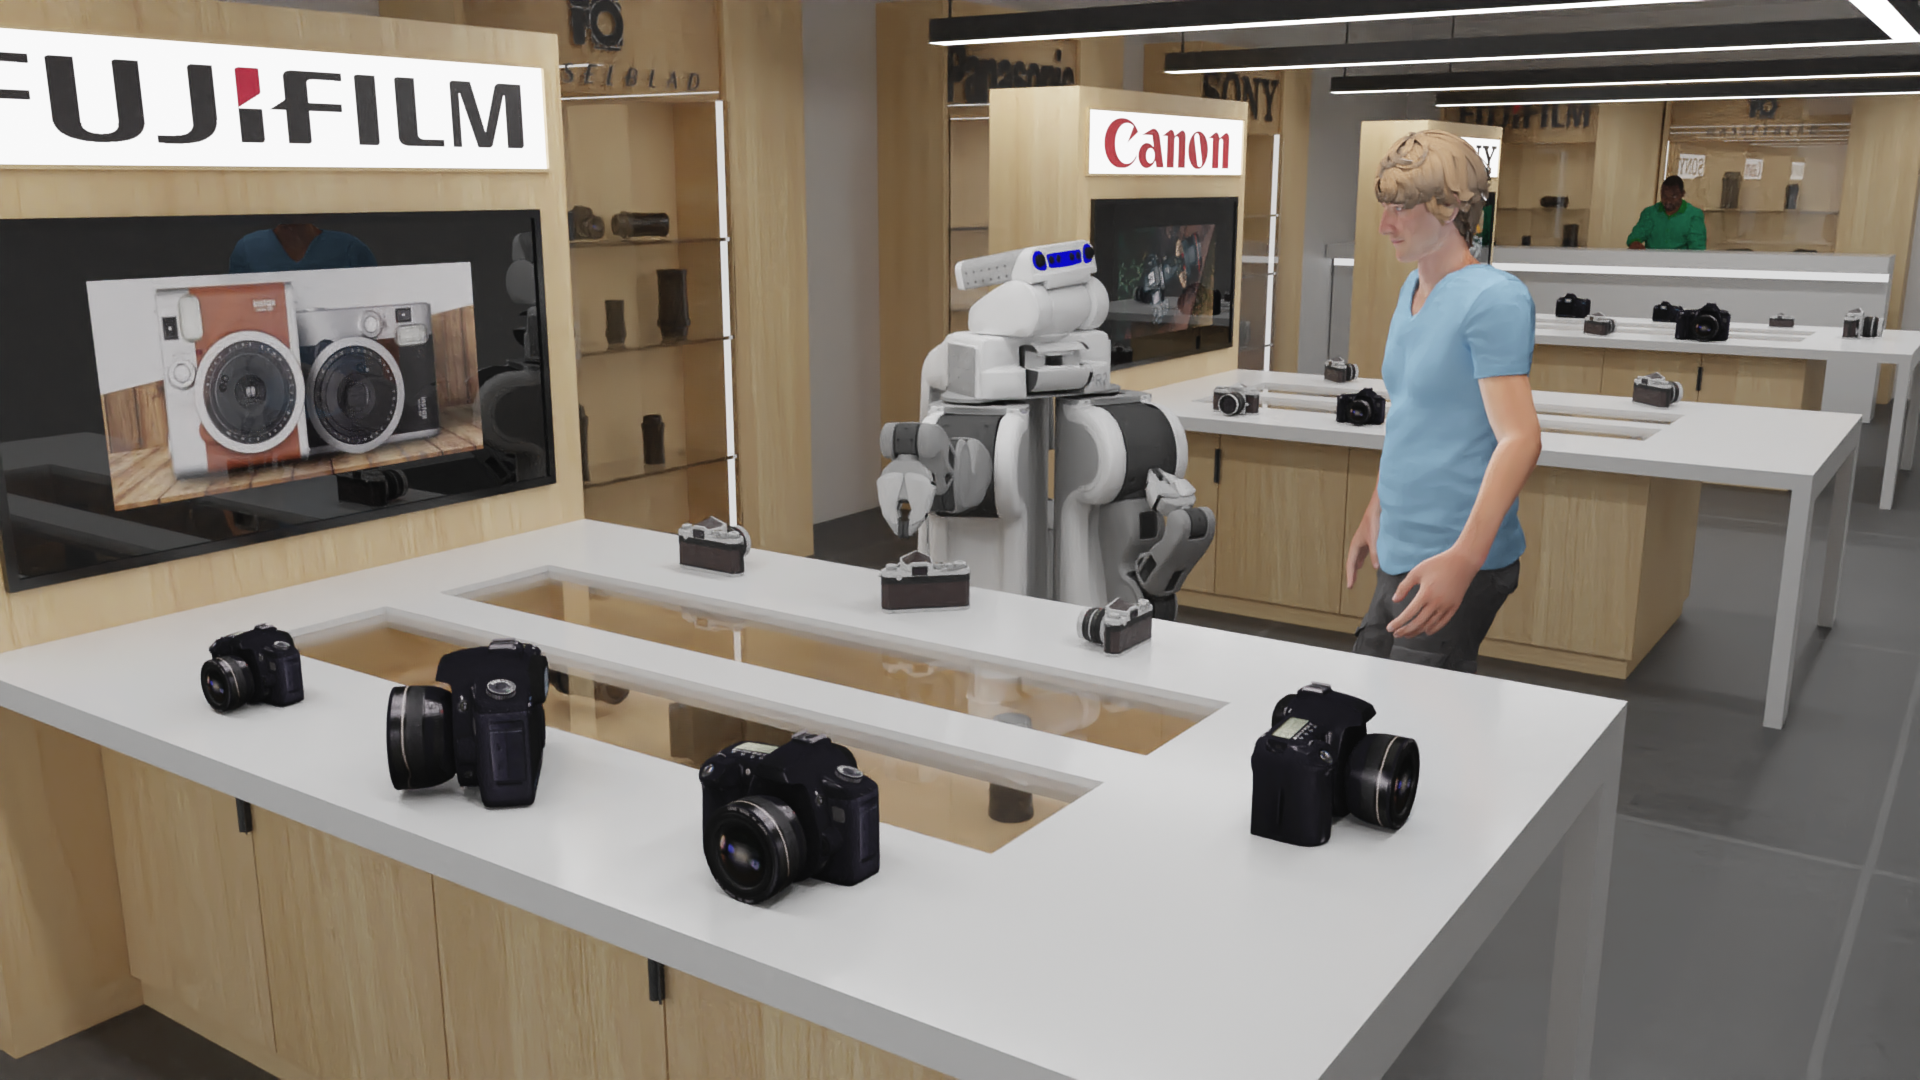
\includegraphics[width=\textwidth]{figures/introduction/camera_store_2.png}
\caption{\label{fig:cam_store} A Pr2 robot, as an employee of a camera store, advises a customer. }
\end{figure}

Explaining that, Max points to the cameras. They continue to discuss when Tony's phone rings. He has to go to join his wife, in another store in the mall. Not knowing where the other store is located, he asks:

\begin{quote}
\textit{
Tony - ``I am sorry I have to go. I will come back in the week. I have to go to a store selling video games but I do not remember the name.'' \\
Max - ``There is only one store selling video games in this mall, it is Game-ania.'' \\
Tony - ``Do you know how to reach it from there ?'' \\
Max - ``For sure''}
\end{quote}

Max moves next to the entrance, followed by Tony. It raises one arm pointing to the aisle and said:

\begin{quote} 
\centering 
\textit{
Max - ``Go down this aisle then turn left straight after the salad bar. After that Game-ania will be on your right when we walk.''}
\end{quote}

Tony leaves and comes back the morning after. Max recognizes him and moves towards him. It asks Tony if he has easily found the video game shop then recalls the camera identified the day before.

\begin{quote} 
\centering 
\textit{
Max - ``Yesterday we stop on two Fujifilm cameras and a Canon for your trip.''}
\end{quote}

They continue to discuss and finally Tony selects the camera at 350 euros. Following Max's advice, he takes a memory card and a second battery to have enough storage and power during his trip. In addition, he takes a zoom lens to take pictures of animals at long range. Unfortunately, the desired camera is not available at the moment. The last one in the store is the demonstration one. Max proposes to Tony to order the camera. The client agrees and leaves.

\begin{figure}[ht!]
\centering
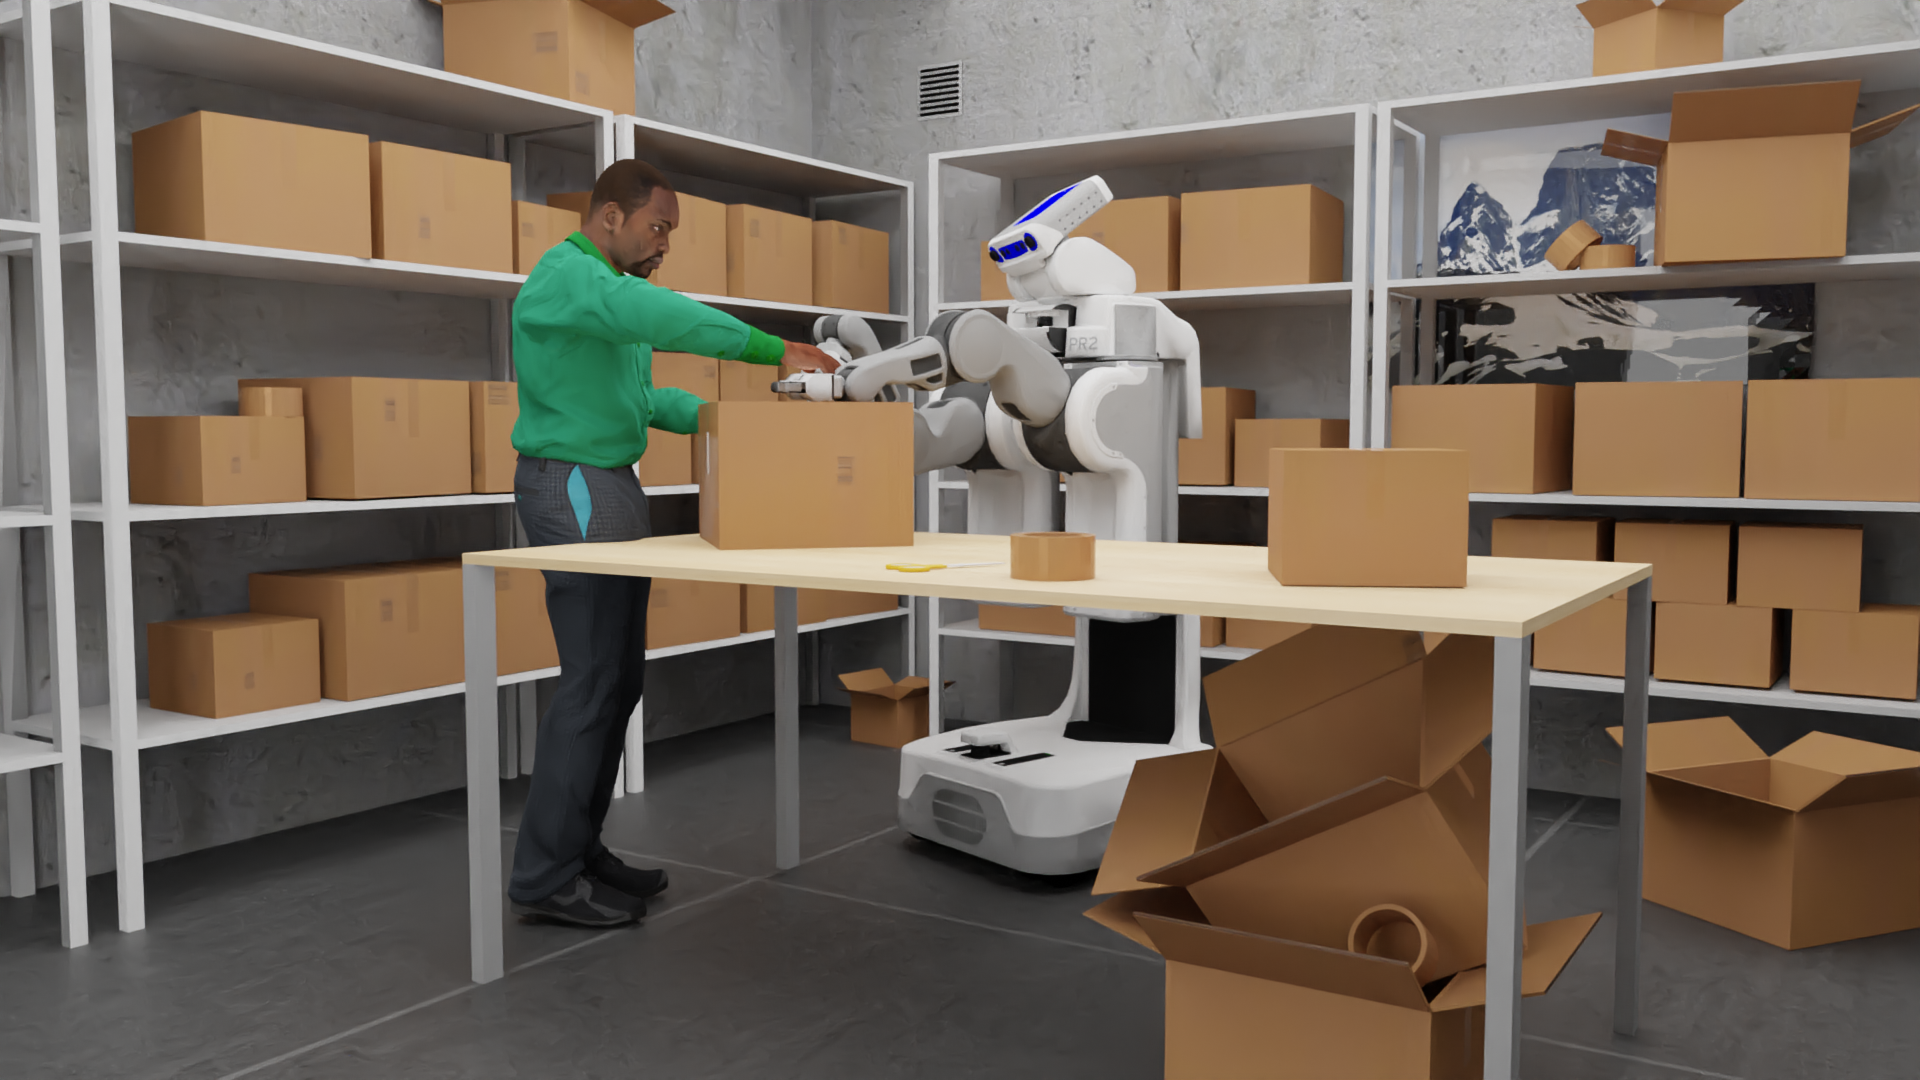
\includegraphics[width=\textwidth]{figures/introduction/camera_store_5.png}
\caption{\label{fig:cam_back} A Pr2 robot and a human employee collaborating to close a box. }
\end{figure}

A few days later, before opening, several boxes are delivered to the store. Liam, the human employee, and Max have to open them, fill stocks and prepare Tony's order. This is the first time since Max arrival they have to do it. They both go to the backroom in order to do this task together. There are two boxes. Liam starts opening one and so Max starts opening the other. Max informs Liam about the camera which has been ordered and is planned to be in the delivery.

\begin{quote} 
\centering 
\textit{
Max - ``Tell me if there is a X-T100, a customer orders one.''}
\end{quote}

Liam finds the camera. The robot explains to him that it also needs an SD card of 32Go and a lens XC 15-45mm. It informs the human that the SD cards are too small for it to grasp them. It thus proposes to Liam to take some of the cameras to put on the shelves and to bring back the card and the lens at the same time. During this time, Max gets a box, puts the camera and the battery inside. When Liam comes back, he puts the two other items in the same box. Then, Max maintains the box close while Liam tapes it. When finished, they both take the last items to put on the shelves and go to the main room.

The afternoon of the same day, while Max is cashing in a customer, Tony enters the store. Seeing him, Max requests Liam:

\begin{quote} 
\centering 
\textit{
Max - ``Can you bring the order we prepared this morning? The client is the one just entering, with the blue T-shirt.''}
\end{quote}

Liam goes to the backroom and brings back the correct box. Max charges the customer who finally gets his camera on time.

\section{Interacting with a robot: What can we expect ?}

Even if the scenario of the robot in a store is not intended to be entirely implemented, it allows us to identify what is needed in terms of knowledge representation, for a robot interacting with humans. First of all, we can draw a rough partition of the needed knowledge:

\begin{enumerate}
  \item \textbf{common-sense knowledge}. It is the knowledge not necessarily related to the current situation but required to understand it. In the scenario, this is not because the robot is in a camera store that it knows the concept of a camera, this concept is more general. Thanks to this common ground it is able to understand the concept of video games, trips, boxes, or animals in our scenario.
  \item \textbf{knowledge of the environment}, grounded in the space. The robot does not only need to know how it can move in its environment, it has to identify the elements composing it, link them to the common ground, and refine them. When Max is powered on for the first time, it goes around the environment to analyse it. Seeing an object, Max identifies it as being a camera. With additional cues, it can refine its knowledge through the model of this camera and its characteristics. This object is on a support, this is a shelf, dedicated to a specific brand, and so on.
  \item \textbf{knowledge of the activities}, grounded in the space and the time. More than how to perform a given task, we are here interested in how it has been achieved. By whom? With whom? Where? When? On which entities? In our scenario, Liam has brought back an SD card from the main room, during this time, Max has prepared a box in the backroom, and these two tasks have been made to prepare, together, Tony's command.
\end{enumerate}

Through this rough partition, we can identify three types of knowledge. The general ones, the knowledge related to space, and those related to time. Where the first can be seen as partially static, all have to be dynamic. The robot should be \textbf{able to gather knowledge}, update it, and create links in between.

At this stage, one can asks: where is the interaction in it? Even if this knowledge is mandatory for a robot interacting with a human, it holds also for a robot acting alone in an environment.

Speaking about interaction, the first use of the knowledge we can think about is communication, meaning sharing information. Consequently, an important property of the robot's knowledge is that a part of it has to be \textbf{narrative-enabled}. The robot should be able to communicate its knowledge. As humans, we can naturally think about verbal communication, for example when it explains the characteristics of the cameras. It can however also be through gestures, like pointing or other dietic gestures. When the robot says ``turn right'' while explaining a route to follow, the language can be accompanied by a hand gesture, turning it on the right. Moreover, for a robot equipped with a screen, we could also imagine communication through texts or images. We claim that only a part of its knowledge has to be narrative-enabled since another part can be dedicated to its internal functioning, from a pure engineering point of view.

When we qualify a piece of knowledge to be narrative-enabled, we can restrict ourselves to communication from the robot and to the human. However, if we consider the robot able to express knowledge, we can assume it to be able to understand it. In this way, in our conception of narrative-enabled knowledge, the robot should be able to formulate sentences and understand humans speech, based on its knowledge. Moreover, to understand its partner the robot not simply has to match the expressed concepts to its knowledge. Since some communications are underspecified, like when the client requests a camera for a trip, the robot can make use of \textbf{inference} to better understand the human. In our scenario, the client explains he is not an expert so the robot advises for an automatic camera. Since he goes on a trip, more storage and battery could be necessary. Since he wants to take pictures of animals, a zoom lens could be useful. All these pieces of information are not explicit to the communication, but thanks to inference on the knowledge can be understood by the robot. Finally, to fully understand its partner, the robot has to consider the \textbf{context} of the entire interaction. When Tony said he wants to acquire a camera at 350 euros, it seems trivial that it is the one at this price among the three previously identified.

Moving toward the knowledge about activities, we have to speak about \textbf{plans}. Keeping it simple for the moment, we can consider a plan as a succession of actions allowing an agent to achieve a task. In this way, a cooking recipe is a kind of plan allowing to achieve the task to prepare a dish. Through the narrative-enabled characteristic of knowledge, we thus want a robot to be able to express a plan. In our scenario, Max asked Liam to bring back an SD card and a lens, it thus expresses a part of a plan. However, it could also have explained to Liam to go in the main room, to move toward the second shelf, to open the rightmost door, to take the SD card in a blue package, and to come back in the backroom. This explanation expresses the same thing but goes deeper into the details, taking a lower level of \textbf{abstraction}. Here we see that the robot has to be able to express a plan at various levels of abstraction. For example, if the robot says ``Let us prepare the order'' it expresses the global task.

Such an explanation of a plan to be carried out highlights a number of key elements regarding the robot's need for knowledge. Here we introduce two of them:

\begin{itemize}
  \item If the robot can express the same plan with different granularity, how does it choose the right one? To answer this question, we have to introduce the self-and-other distinction. To know which information to share, a robot has to \textbf{estimate its partner knowledge}, that it is the common-sense knowledge as well as the knowledge about the environment and the activities. It is on the basis of this estimation that the robot can know how to communicate. In our scenario, the robot interacts with the human employee to prepare the order. Since Liam was in the store before the robot, it could estimate that the employee knows where the SD cards are. Communicating this low-level information would thus be useless and inefficient for the task. The human employee would be a new one, the robot would have interacted in a different way. This estimation of the others knowledge can be found somewhere else in the scenario. When Max refers to a specific camera to the client, it describes it in relation to its attributes and location. To the difference, to refer to the same entities to Liam, Max uses the precise model name of the camera. It thus estimates that the client does not know the model's name but that the employee does.
  
  \item To allow the robot to communicate at the right level of abstraction, estimating the other knowledge allows the detection of \textbf{belief divergence}. It appears when the robot estimates that the other does not have a piece of knowledge or still considers a piece of knowledge that no more holds. Detecting such a divergence can be used to prevent errors for example. In our scenario, if the robot has taken the last zoom lens on a given shelf and estimates that the employee is not aware of this information, it can detect a belief divergence. Consequently, rather than just asking for a zoom lens, it can inform the other that there is no more lens at this place. The employee will no have to search at the original place and will be able to directly go to another place where there is still some zoom lens.
\end{itemize}

Continuing to explore the knowledge implies by the realisation of a plan, we can move toward the elaboration of the plan, the planning of the task. By achieving the task together, the human and the robot are performing a \textbf{joint-task}, meaning having a joint-goal and collaborating to achieve it. To collaborate the robot elaborates a \textbf{plan considering the human}. It can thus propose to him to achieve a part of the task. To know how to dispatch the actions, the robot needs knowledge about \textbf{human abilities} as well as its own abilities. In the scenario, the SD card is assigned to the human because the robot is aware that it can not grasp it. If the object to bring back was graspable by it, maybe it would have done it by considering it as uncomfortable for the human to walk too much. Underlying, this ability to plan for himself and others also requires a projection into future situations and thus a \textbf{representation of possible worlds state}, like what is done in task planning.

Finally, the human is not an agent like the robot, he can not be controlled. Even if the robot plans by considering him, the human can act freely. The robot thus has to \textbf{monitor, interpret, and ground human actions}. From there and with regard to the plan and thus the joint-task, it can react and adapt. In our scenario, when Liam starts opening one of the two boxes, the robot adapts and takes the other one, even if it planned a different course of action. In this situation inverting does not raise any issue, they can thus continue.

In this section, we have identified some of the key elements need and use about knowledge for \acrfull{hri}. Even if we were not able to tackle all of them in this thesis, they give the context in which the presented contributions have been thought and they aim to be integrated. In this section, we have often use the term ``knowledge''. However under this general term can be found a number of concepts related to memory and how, as humans, we are able to remember things. Before moving to the contributions of this thesis, we propose in the next section an overview of some model from the cognitive psychology, allowing to better understand how we represent our knowledge.

\section[Knowledge organization]{Knowledge organization: Drawing inspiration from cognitive psychology }

Even if our goal in robotics is not to create a copy of the human, either in terms of body shape or cognition, drawing inspiration from it is nevertheless important. In the same way that roboticists take inspiration from the human body to create robots able to act in a world created by and for the human, the field of cognitive robotics takes inspiration from the human cognition to create robots able to interact with humans. While we do not aim to imitate human cognition, we think that a robot must be endowed with some similar capabilities if we want them to interact with us efficiently and in an acceptable way.

Regarding the knowledge representation, the first experimental study has been realized in 1885 by Ebbinghaus~\cite{ebbinghaus_1885_gedachtnis}. Since then, the definition of memory as the capacity to encode, store, and retrieve knowledge \cite{roediger_1996_retrieval} has been widely accepted. At the same time, the word ``memory'' has become a generic term suggesting a unique system. However, the human memory can rather be seen as several sub-systems that differ from their storage duration, storage capacity, and the level of consciousness necessary for information retrieval. In the rest of the section, we present some memory models, presented in a non-chronological way, and focussing on what is called long-term memory. During all this section, it is important to keep in mind that we only present models aiming to understand human cognition with a focus on knowledge management. No formal truth is stated here given that there is no consensus in the field. The presented models and terms will allow us to better understand the existing robotic cognitive architectures and give inspiration for the design and structuring of the components developed in this thesis.

The primary division of the memory is done concerning the storage duration and capacity. From there has been defined the \textbf{short-term memory} (STM) and the \textbf{long-term memory} (LTM) \cite{atkinson_1966_some}. Short-term memory is characterized by its small capacity and its capability to retrieve information that has just been seen. It is often stated that it is near to twenty seconds and seven items (or chunks)\cite{miller_1956_human}. Long-term memory, on the opposite, refers to any situation where we use information that has not just been seen. It is often stated that it has an infinite capacity and duration. It is this latter that allows the acquisition of new knowledge and the retrieval of information acquired a long time ago.

Over the years, what was called short-term memory has become the \textbf{working memory} (WM) \cite{baddeley_1986_dementia}. This change has been made to add a notion of knowledge manipulation. Instead of focusing on the only temporal aspect, it reflects its functional aspect. It is thus a system that retains information for the time necessary for its use by other cognitive functions. The working memory and the long-term memories are two independent but related systems. For information to be stored in long-term memory, we think that it has to pass by the working memory.

For the structure of the long-term memory, a first dichotomy is proposed by Graf and Schacter \cite{graf_1985_implicit} with the \textbf{implicit} and \textbf{explicit} memory. It reflects the way knowledge can be retrieved. Knowledge from explicit memory can be retrieved consciously and voluntarily. On the opposite, knowledge from implicit memory is retrieved in situations in which our behaviors are influenced by an experience. This is the case when one pours water into a glass. We do not need to retrieve explicitly how to perform this task. It is our experience that influences how we do it.

Another dichotomy has been proposed by Squire and Cohen \cite{squire_1982_remote} with the \textbf{procedural} and \textbf{declarative} memory. Procedural memory is the system allowing us to retain knowledge about our cognitive, motor, or perceptual skills. It is the memory of the know-how. A specificity of this memory is that it is difficult to verbalize the knowledge it stores and we use them unconsciously. The declarative memory stores representations of facts, events, general knowledge, and memories of past events. This knowledge can be retrieved consciously and we can speak about them. Taking the example of the code of your credit card. Initially, this knowledge is stored in the declarative memory. When you need it, you can easily remember it and say it. The more you use it and it slowly becomes an automatism. It became hard to remember it consciously while you use it every day and if you need to say it you need to type it on a virtual keyboard to remember it. It has slowly moved into your procedural memory. We see that both dichotomies are almost equivalent. The declarative memory of Squire is related to the implicit memory of Graf, and the procedural one is related to the implicit memory.

Going deeper into the declarative memory, Tulving has proposed a dichotomy between \textbf{episodic} and \textbf{semantic} memory \cite{tulving_1995_organization}. The episodic memory retains knowledge related to past experienced events, which are specific to our individual experience, and localized both in space and time. The semantic memory is more general and retains knowledge that we accumulate all along with our life concerning our environment. It can be seen as an encyclopedic memory independent of the acquisition context. While the episodic memory is related to ``remembering'', the semantic one is related to ``knowing''. Taking as an example your visit to Toulouse \footnote{If you never visit it, you can take another city you have visited but you should plan to visit it anyway.}, this visit is encoded in the episodic memory while the knowledge that Toulouse is a city in France is encoded in the semantic one.

\begin{figure}[h!]
\centering
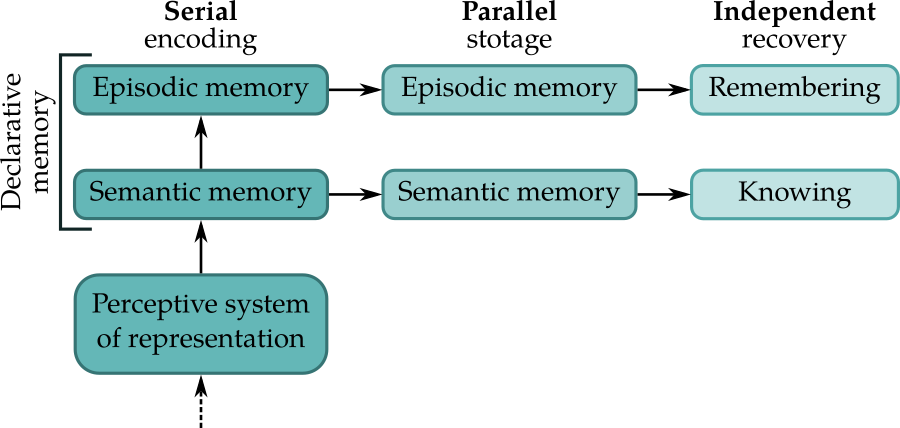
\includegraphics[scale=0.45]{figures/introduction/SPI.png}
\caption{\label{fig:SPI} Relations between episodic memory and semantic memory according to the SPI (Serial, Parallel, and Independent) model of Tulving (1995).}
\end{figure}

With the previous example, we saw that even if these two sub-systems of the declarative memory are independent, they are therefore in interaction with each other as we can apply a semantic treatment on the episodic memory. To better understand their relation, Tulving has proposed the Serial, Parallel, and Independent model (SPI). As illustrated in Figure~\ref{fig:SPI}, the encoding of information is serial (S) passing first by the semantic memory, then in the episodic one. The storage in both memories is performed in parallel (P). Finally, the information recovery is independent between the two memories.
As we explain at the beginning of this section, the presented theory can not be proven and must therefore be taken as~\cite{tulving_1995_organization} ``an explicit starting point for a more systematic pursuit of what is clearly the next problem that needs to be tackled''.

For this thesis, and robotic in general, these hypotheses about the knowledge organisation for humans allows a better understanding of the kind of knowledge we have to manage. We have identified three types: semantic, episodic, and procedural. Wanting to insert a new piece of knowledge, we can thus identify the types it is of and thus where to store it.

\section{Contributions}

This section summarizes the main contributions of this thesis. They are organised around three complementary topics: knowledge management, knowledge exploitation, and cognitive architectures. All have been thought in the context of \acrlong{hri}, meaning what a robot needs to take the human into account and interact with him.

\subsection{Knowledge management}

The starting point of this thesis is the need to store and maintain both the robot's and humans' estimated knowledge. We focused our efforts on semantic knowledge, using an ontology to represent it. The core contribution of this thesis is thus a software component to manage ontology instances. Each instance represents an agent knowledge, with the robot one being its ``ground truth''\footnote{This is the knowledge about what has been directly perceived by the robot.} and its partners' ones being an estimation of their knowledge\footnote{Either estimated to be perceived by the human or explicitly provided by the programmer.}. The ontology is used to represent the common-sense knowledge, the knowledge about the environment, knowledge about activities, as well as knowledge for the proper functioning of the robot.

The resulting software is called Ontologenius. It is a lightweight and open-source software developed in C++ and working as a server within a robotic architecture. Any component of the architecture can thus access the knowledge it maintains through the ROS middleware, ensuring uniformity of the knowledge among the entire architecture. It comes with extensive documentation, debugging tools, and an API in C++ and python.

Ontologenius supports dynamic updates of the \acrlong{kb}s it maintains and keeps them consistent at any instant thanks to reasoners. At the date, five main reasoners are available in the form of plugins, each dedicated to a specific axiom. Others can thus be added depending on the need. They can be activated or deactivated at runtime and propose different reasoning managements. We can for example choose to run then upon the query, at an update or periodically. Ontologenius is able to make the difference between a stated fact and a deduced one.

At the difference of other ontology management software, Ontologenius comes with more than 60 low-level inbuilt parametrizable queries, allowing a fast and precise exploration of the knowledge. These queries have been designed in such a way to be called from search algorithms to create higher-level cognitive processes. In addition, it proposes a \sparql{} interface.

Ontologenius has also been designed to be used for task planning applications by representing several possible world states in a single instance, switching from one to another.

It was made from scratch and thought like a sandbox, based on ontology standards but sometimes allowing to deviate from them to better explore the possibilities and never be limited.

During this thesis, a software to manage episodic knowledge has also been developed and linked with Ontologenius. It is called Mementar. Due to its early stage, it will not be presented in-depth but used in the final contribution of this thesis. 

\subsection{Knowledge exploitation}

On the basis of the semantic knowledge management software Ontologenius, several knowledge exploitation contributions have been developed. We can group them all into the topic of spatial referring.

The first tackles the route description task. Describing an indoor environment using an ontology, we have proposed two complementary algorithms able to find several routes leading to a target place. To represent an indoor environment with an ontology, we have proposed a piece of ontology to describe the topology, called the \acrlong{ssr}. It allows the description of the static elements of the environment, perceptible by humans, as well as elements necessary for the verbal description of a route. We have then developed an algorithm to verbalise routes, respecting good practices.

The second tackles the \acrlong{reg} task. The goal is to search for the knowledge to communicate to a hearer allowing him to identify the target entity without ambiguity, in a given context. The resulting algorithm has been shown as being the most efficient to date, even if the input \acrshort{kb} is not dedicated to the task. This contribution has been an important source of inspiration and has lead to three other related contributions. We have linked this algorithm to a symbolic task planner to evaluate communication feasibility and cost during the planning process. After this link with a planner, we tried to exploit the shared Human-Robot experience as a new kind of knowledge usable to generate \acrlong{re}. The latter contribution leads us to a proposal of task representation in an ontology. To move toward a more generic method to generate \acrlong{re}, we finally start a preliminary work aiming to support n-ary relations.

\subsection{Cognitive architectures}

The last contributions of this thesis are two cognitive architectures embodied on a Pepper and a Pr2 robotic platforms. The first architecture has been developed in the context of the \acrlong{mummer} project. It makes use of the route description to guide customers in a mall. The second has been developed later at LAAS-RIS to experiment recent developments of the team. This architecture makes use of the contributions around the \acrlong{reg}. It has been tested in a task inspired by cognitive psychology and adapted to the \acrlong{hri}, called the Director Task.

Both architectures use Ontolognenius to manage the robot and humans semantic \acrshort{kb}s. Since both architectures were developed two years apart, we will see in this thesis how the semantic \acrlong{kb} has become a central element of our cognitive architecture for \acrlong{hri}.

\section{A reader's guide}

\subsection*{Thesis organisation}

This thesis is partly based on published or submitted work. Some of the key contributions are more detailed than the paper version, while work involving several students is rather summarized to provide an overview of an integrated contribution.
This thesis is organised in an almost progressive way. Such an organisation aims at following step by step the way in which each contribution has been thought about regarding the previous ones. For example, from Chapter \ref{chap:5} to Chapter \ref{chap:7} an architecture is built proposing each time the integration of new components and new abilities. 

This thesis is organized into three parts: knowledge management, knowledge exploitation through referring applications, and finally the integration into robotic architectures. The knowledge management is presented in Chapter~\ref{chap:ontologenius} with the software Ontologenius. This software is then the core of all the other contributions. The knowledge exploitation has been studied with referring tasks. Chapter \ref{chap:3} proposes a knowledge representation and algorithm to describe routes for guide robots. Chapters \ref{chap:4} to \ref{chap:7} are all around the \acrlong{reg} problem. This thesis ends with two robotic architectures embodied respectively into a Pepper and a Pr2 robotic platform. The first architecture has been developed approximatively from 2017 to 2019 in the context of a European project. The second architecture is an internal project of the team, giving more flexibility to explore new designs and new organisation of its components. The latter has been developed from 2020 to 2021. While the first architecture uses the route description knowledge exploitation, the second use the contributions on the \acrlong{reg}. Having these two architectures grouped at the end of this thesis allows us to compare them and see how knowledge management has taken a primary place in a robotic architecture for \acrlong{hri} applications.

All along this thesis, special attention has been paid to the performance of each contribution. Each time our aim is to integrate the presented contribution into a wider system and work in an incremental manner. To not spoil the final Human-Robot interaction and be able to create more high-level cognitive capabilities, this attention is essential to us. At the end of most of the chapter, a performance analysis is thus provided.

\subsection*{To get to the point}

For the readers having less time and wanting to go to the point of this thesis, we can propose a shorter reading route. For sure, this selection is subjective, we often prefer our latter work, which seems to us more mature, having a better background on the topics. We thus suggest to read to following:

\begin{itemize}
  \item Chapter \ref{chap:ontologenius}: Ontologenius, the ontology management software, the core of this thesis,
  \item Chapter \ref{chap:4}: The \acrlong{reg} algorithm,
  \item Introductions of chapters \ref{chap:5} and \ref{chap:6}: Some challenges around the \acrlong{reg},
  \item Chapter \ref{chap:7}: A preliminary work to create more generic \acrlong{re}s,
  \item Section \ref{sec:9_3}: Our most advanced cognitive architecture for \acrlong{hri} applications.
\end{itemize}

\subsection*{List of Publications}
\markright{LIST OF PUBLICATIONS}
\subsubsection*{Published}
\begin{itemize}
\item Sarthou, G., Alami, R., \& Clodic, A. (2019, June). Semantic Spatial Representation: a unique representation of an environment based on an ontology for robotic applications. In Combined Workshop on Spatial Language Understanding (SpLU) and Grounded Communication for Robotics (RoboNLP).

\item Sarthou, G., Clodic, A., \& Alami, R. (2019, October). Ontologenius: A long-term semantic memory for robotic agents. In 2019 28th IEEE International Conference on Robot and Human Interactive Communication (RO-MAN) (pp. 1-8). IEEE.

\item Heikkilä, P., Lammi, H., Niemelä, M., Belhassein, K., Sarthou, G., Tammela, A., Clodic, A.,  \& Alami, R. (2019, November). Should a robot guide like a human? A qualitative four-phase study of a shopping mall robot. In International Conference on Social Robotics (pp. 548-557). Springer, Cham.

\item Buisan, G.*, Sarthou, G.*, Bit-Monnot, A., Clodic, A., \& Alami, R. (2020, August). Efficient, situated and ontology based referring expression generation for human-robot collaboration. In \textit{2020 29th IEEE International Conference on Robot and Human Interactive Communication (RO-MAN)} (pp. 349-356). IEEE.

\item Buisan, G., Sarthou, G., \& Alami, R. (2020, November). Human aware task planning using verbal communication feasibility and costs. In \textit{International Conference on Social Robotics} (pp. 554-565). Springer, Cham.
\end{itemize}

\subsubsection*{Accepted}

\begin{itemize}
\item Sarthou, G., Mayima, A., Buisan, G., Belhassein, K., \& Clodic, A. The Director Task: a Psychology-Inspired Task to Assess Cognitive and Interactive Robot Architectures. To be published in \textit{2021 30th IEEE International Conference on Robot and Human Interactive Communication (RO-MAN)}.

\item Sarthou, G., Buisan, G., A., Clodic, A., \& Alami, R. Extending Referring Expression Generation through shared knowledge about past Human-Robot collaborative activity. In \textit{2021 IEEE/RSJ International Conference on Intelligent Robots and Systems (IROS)}
\end{itemize}

\subsubsection*{Submitted}

\begin{itemize}
\item Mayima, A., Sarthou, G., Buisan, G., Singamaneni, P., Sallami, Y., Belhassein, K., Waldhart, J., Clodic, A., \& Alami, R. Direction-giving considered as a Human-Robot Joint Action. Submitted to \textit{User Modeling and User-Adapted Interaction (UMUAI) Journal}.
\end{itemize}
\ifdefined\included
\else
\setcounter{chapter}{1} %% Numéro du chapitre précédent ;)
\dominitoc
\faketableofcontents
\fi

\chapter{State od the art}
\minitoc

Lorem ipsum dolor sit amet, consectetur adipiscing elit. Sed non risus. Suspendisse lectus tortor, dignissim sit amet, adipiscing nec, ultricies sed, dolor. Cras elementum ultrices diam. Maecenas ligula massa, varius a, semper congue, euismod non, mi. Proin porttitor, orci nec nonummy molestie, enim est eleifend mi, non fermentum diam nisl sit amet erat. Duis semper. Duis arcu massa, scelerisque vitae, consequat in, pretium a, enim. Pellentesque congue. Ut in risus volutpat libero pharetra tempor. Cras vestibulum bibendum augue. Praesent egestas leo in pede. Praesent blandit odio eu enim. Pellentesque sed dui ut augue blandit sodales. Vestibulum ante ipsum primis in faucibus orci luctus et ultrices posuere cubilia Curae; Aliquam nibh. Mauris ac mauris sed pede pellentesque fermentum. Maecenas adipiscing ante non diam sodales hendrerit.

\section{Congnitive architectures and underlying knowledge representations}

\section{How reasoning can expand the knowledge}

\section{Knowlege exploitation for service robotics}

\section{Knowlege exploitation for Human-Robot Interaction}

Lorem ipsum dolor sit amet, consectetur adipiscing elit. Sed non risus. Suspendisse lectus tortor, dignissim sit amet, adipiscing nec, ultricies sed, dolor. Cras elementum ultrices diam. Maecenas ligula massa, varius a, semper congue, euismod non, mi. Proin porttitor, orci nec nonummy molestie, enim est eleifend mi, non fermentum diam nisl sit amet erat. Duis semper. Duis arcu massa, scelerisque vitae, consequat in, pretium a, enim. Pellentesque congue. Ut in risus volutpat libero pharetra tempor. Cras vestibulum bibendum augue. Praesent egestas leo in pede. Praesent blandit odio eu enim. Pellentesque sed dui ut augue blandit sodales. Vestibulum ante ipsum primis in faucibus orci luctus et ultrices posuere cubilia Curae; Aliquam nibh. Mauris ac mauris sed pede pellentesque fermentum. Maecenas adipiscing ante non diam sodales hendrerit.

Ut velit mauris, egestas sed, gravida nec, ornare ut, mi. Aenean ut orci vel massa suscipit pulvinar. Nulla sollicitudin. Fusce varius, ligula non tempus aliquam, nunc turpis ullamcorper nibh, in tempus sapien eros vitae ligula. Pellentesque rhoncus nunc et augue. Integer id felis. Curabitur aliquet pellentesque diam. Integer quis metus vitae elit lobortis egestas. Lorem ipsum dolor sit amet, consectetuer adipiscing elit. Morbi vel erat non mauris convallis vehicula. Nulla et sapien. Integer tortor tellus, aliquam faucibus, convallis id, congue eu, quam. Mauris ullamcorper felis vitae erat. Proin feugiat, augue non elementum posuere, metus purus iaculis lectus, et tristique ligula justo vitae magna.
Aliquam convallis sollicitudin purus. Praesent aliquam, enim at fermentum mollis, ligula massa adipiscing nisl, ac euismod nibh nisl eu lectus. Fusce vulputate sem at sapien. Vivamus leo. Aliquam euismod libero eu enim. Nulla nec felis sed leo placerat imperdiet. Aenean suscipit nulla in justo. Suspendisse cursus rutrum augue. Nulla tincidunt tincidunt mi. Curabitur iaculis, lorem vel rhoncus faucibus, felis magna fermentum augue, et ultricies lacus lorem varius purus. Curabitur eu amet.

\ifdefined\included
\else
\setcounter{chapter}{2} %% Numéro du chapitre précédent ;)
\dominitoc
\faketableofcontents
\fi

\chapter{Ontologenius: A long-term semantic memory}
\minitoc

\section{Design and features}

\subsection{Why an ontology?}

\subsection{Ontology formalism}

Even if we saw that the use of ontology is today a common way to represent semantic knowledge, we will recall in this subsection the composition of an ontology. For each element composing it, we will draw a formalization then give examples using the Turtle syntax. The pieces of ontologies used in the examples of this subsection are voluntarily simplified. The introduced notations will be the ones used in the rest of this thesis and the graphical representations, both in terms of color and form, will be kept as often as possible.

On the base of the definition of a Description Logic ontology presneted in \cite{fokoue_2006_summary}, we define a semantic knowledge base $\kbs$ represented as an ontology by  $\kbs = \langle \Abox, \Tbox, \Rbox \rangle$. $\Abox$, $\Tbox$, and $\Rbox$ are respectively called the Abox, Tbox, and Rbox of the ontology.


\begin{figure}[h!]
\centering
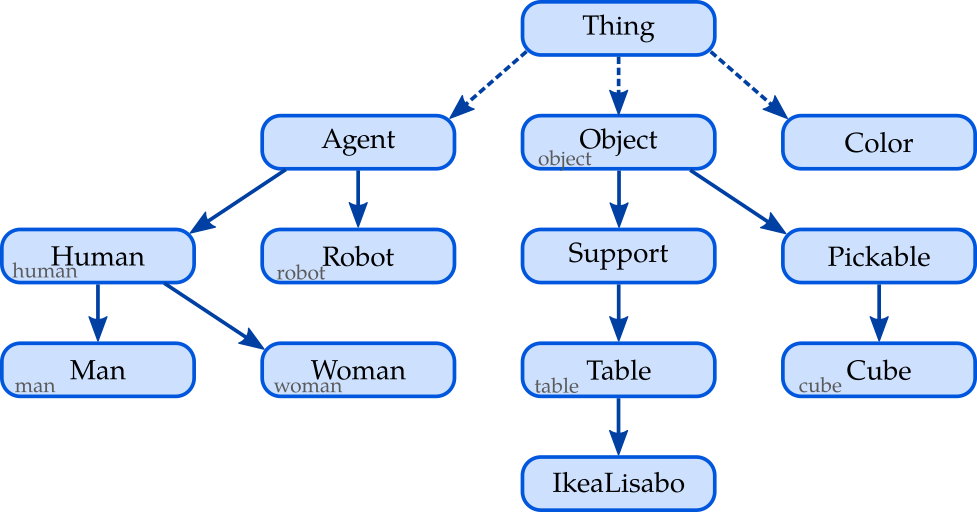
\includegraphics[scale=0.4]{figures/chapter2/Tbox.png}
\caption{\label{fig:Tbox} Representation of an ontology class hierarchy graph to illustrate the composition of a TBox. Taking the class Human, the bottom arrow has to be read as \textit{"A man is a kind of Human"}. The texts at the bottom left of the class, if there is, are the classes' labels in natural language.}
\end{figure}

The Tbox $\Tbox$ contains assertions about the \textbf{classes} (types) of the ontology. It is defined by $\Tbox = \langle \classset, H \rangle$. It can be seen as a directed acyclic graph as presented in Figure~\ref{fig:Tbox}. $\classset$ is the set of all the classes of the ontology. In our example, $\classset = \{Thing,\ Agent,\ Object, ...,\ IkeaLisabo\}$. Considering the Tbox as a graph, $H$ stores its directed edges. It represents the inheritance links between the classes (i.e. the subsumption assertions). This link is commonly referred to as the "isA" link (e.g. \textit{(Human, isA, Agent)}) and is described with the property rdfs:subClassOf in the OWL language as illustrated in the Listing~\ref{lst:Tbox}.

\begin{lstlisting}[frame=single, basicstyle=\scriptsize\ttfamily, label={lst:Tbox}, caption={Description of ontology classes in the OWL language using the Turle syntax.},captionpos=b]
:Human rdf:type owl:Class ;
       rdfs:subClassOf :Agent .

:Man   rdf:type owl:Class ;
       rdfs:subClassOf :Human .
\end{lstlisting}

\begin{figure}[h!]
\centering
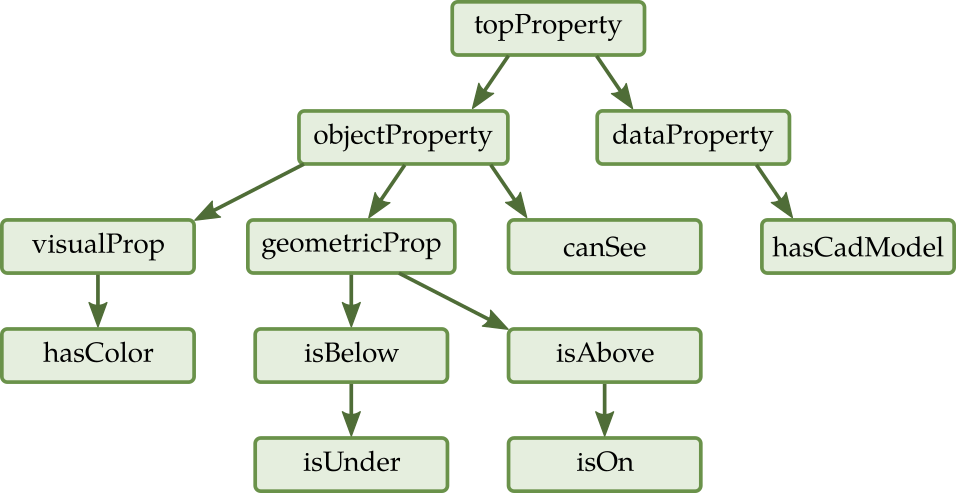
\includegraphics[scale=0.4]{figures/chapter2/Rbox.png}
\caption{\label{fig:Rbox} Representation of an ontology property hierarchy graph to illustrate the composition of an RBox. Taking the property isBelow, the bottom arrow has to be read as: \textit{"The property isUnder is a specification of the property isBelow"}.}
\end{figure}

The Rbox $\Rbox$ contains assertions about the \textbf{properties} (roles). It is at least defined by $\Rbox = \langle \propset, \inclset, \invset, \domainset, \rangeset \rangle$. In the same way as the Tbox, $\propset$ is the set of properties, and $\inclset$ stores the directed edges of the finite directed acyclic graph representing the inheritance links between the properties. Such a graph is represented in Figure~\ref{fig:Rbox}. These inheritance links aim at specifying properties. In our example, the property IsOn is a specification of the property isAbove in the way that an object being on another is an object that is above the latter and being in contact with. It is described with the property rdfs:subPropertyOf in the OWL language. 
$\invset = \{(\property, \property^{-1}) \in \propset^2\}$ is the set representing the properties inverses (\textit{e.g.} $(isOn, isUnder) \in Inv$). Describing the inverse of a property is useful first to reduce description work since if some describe a relation involving a property for which an inverse is defined, the inverse relation is also described in an underlying way. Moreover, for an algorithm exploring an ontology, knowing that a relation uses a property having an inverse can allow reducing the algorithm complexity by not considering the inverse relation into the exploration.
Finally, $\domainset$ and $\rangeset$ are two sets representing respectively the properties domains and ranges. Their are define by $\domainset = \{(\property, \class)\}$ and $\rangeset = \{(\property, \class)\}$ with $\property \in \propset$ a property and $\class \in \classset$ a class. The domain of a property informs on the type of resources that may use the property, thus the type of the subject of a triplet. The range of a property informs on the valid values applied to the property, thus the type of the object of a triplet. For the property isOn, we would therefore have $(isOn,\ Object) \in \domainset$ and $(isOn,\ Support) \in \rangeset$. In this way, we state that the property IsOn can be used to describe that an object is on top of an object being support. Domains and ranges can be used in two ways. It can be to check the consistency of an ontology by checking if the way the properties have been used corresponds to their definition. It can also be used to reason on the ontology and extract new knowledge from a given situation. If, for example, an entity is said to be on top of another that is not described as being a support, we could deduce that this second entity may be a support.

The formalization above considers only a general kind of property while the OWL language makes the distinction between two main categories. The \textbf{object properties}, linking two entities, and \textbf{data properties}, linking an entity to a value. While both are slightly different, we will only keep a general definition of a property for our formalization to simplify the future algorithm explanations. An example of the description of an object property and a data property from the Figure~\ref{fig:Rbox} are illustrated in the Listing~\ref{lst:Rbox} using the OWL language.


\begin{lstlisting}[frame=single, basicstyle=\scriptsize\ttfamily, label={lst:Rbox}, caption={Description of ontology properties in the OWL language using the Turle syntax.},captionpos=b]
:isOn  rdf:type owl:ObjectProperty ;
       rdfs:subPropertyOf :isAbove ;
       owl:inverseOf :isUnder ;
       rdfs:domain :Object ;
       rdfs:range :Support .

:hasCadModel rdf:type owl:DatatypeProperty ;
             rdfs:domain :Object .
\end{lstlisting}

\begin{figure}[h!]
\centering
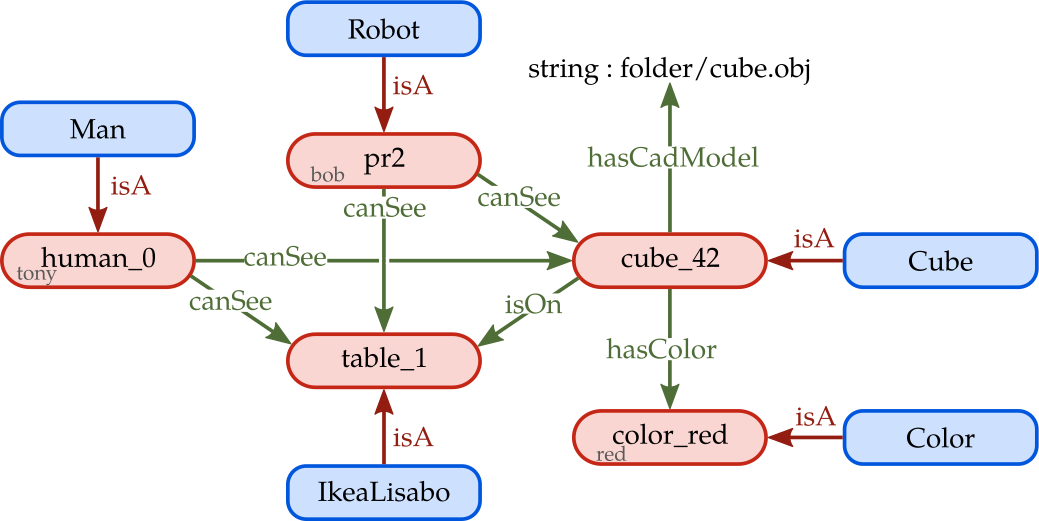
\includegraphics[scale=0.4]{figures/chapter2/Abox.png}
\caption{\label{fig:Abox}  Representation of an ontology instances graph to illustrate the composition of an ABox. Red boxes are individuals of the ontology. Green arrows are properties coming from the RBox and applied to individuals. Red arrows represent a direct inheritance link between an individual and a class coming from the TBox. The texts at the bottom left of the individuals, if there is, are the individuals' labels in natural language.}
\end{figure}

The Abox $\Abox$ contains assertions about the \textbf{entities} (individuals) of the ontology. When we refer about entities, we no more speak about general concepts but rather of instantiated concept, being either a physic or virtual entity. The Abox is defined by $\Abox = \langle \indivset, \inheritset_0, \relationset \rangle$. $\indivset$ is the set of all the entities represented in the ontology. $\inheritset_0$ the set of direct types of $\indivset$ such as $\inheritset_0 = \{(\indiv, \class) \}$ with $\indiv \in \indivset$ an individual and $\class \in \classset$ a class. In the graphical representation of an Abox in the Figure.~\ref{fig:Abox}, the red blocks are the Abox entities ($\indivset = \{human_0,\ pr2,\ ...,\ table\_1\}$) and the red arrows with the label "isA" are the intities direct types ($(cube\_42, Cube) \in \inheritset_0$).
$\relationset$ is finally the set of \textbf{relations} between entities. Such relation are in the form of triplets $(\subject, \property ,\object)$ where $\subject$ is the subject, $\property$ the property and $\object$ the object. The set of relations is thus defined by $\relationset = \{(\subject, \property ,\object) | (\subject, \object) \in \indivset^2, \property \in \propset\}$. These relations are represented by the green arrows between the entities in Figure~\ref{fig:Abox}. We can note in this figure the presence of the use of a data property "hasCadModel". This property does not link two entities, which goes against the previous definition. Regarding our formalization and to keep it tractable, we can however keep it as it is, and view the string value as an entity having for direct type a concept "String". An example of the description of an entity from the Figure~\ref{fig:Abox} is illustrated in the Listing~\ref{lst:Abox} using the OWL language.

\begin{lstlisting}[frame=single, basicstyle=\scriptsize\ttfamily, label={lst:Abox}, caption={Description of an ontology individual in the OWL language using the Turle syntax.},captionpos=b]
:cube_42  rdf:type     :Cube ;
          :hasColor    :color_red ;
          :hasCadModel "folder/cube.obj"^^string ;
          :isOn        :table_1 .
\end{lstlisting}


We just saw that in the Abox, $\inheritset_0$ contains the direct types of entities. We also saw that the classes can inherit from one each other in the Tbox, thanks to the classes inheritance directed edges stored in $H$. This means that the individuals of the Abox have inherited types. Taking the entity cube\_42 of Figure.~\ref{fig:Abox}, its direct type is the class Cube ($(cube\_42,\ Cube) \in \inheritset_0$). Regarding the Tbox represented in Figure.~\ref{fig:Tbox}, a Cube is a kind of Pickable ($(Cube,\ Pickable) \in H$), itself being a kind of Object ($(Pickable,\ Object) \in H$). We can thus say that the entity cube\_42 is a Cube, a Pickable, and an Object. To represent it, we use $\inheritset$ to denote the set of direct and inherited types. We thus have $\{ (cube\_42,\ Cube), (cube\_42,\ Pickable), (cube\_42,\ Object)\} \subset \inheritset$.

With the use of the relation set $\relationset$ of the Abox we saw that we can apply properties to individuals to link them together and form relations in the form of triplets. However, some could want to apply properties to classes to describe general links between classes. While properties domains and ranges already give such relations this can be not enough. Taking an object property hasMother, we can assign to it the class Human for domain and Woman for range. With such description, we state that a human CAN have a mother that is a woman but we do not describe that even if we do not know how it is, a human has a mother how is a woman. For this particular example, we could use cardinality constraint but we will not go as far. Taking now the data property hasCadModel of Figure~\ref{fig:Rbox}, we have applied it to a specific entity in the example of Figure~\ref{fig:Abox}. But what about a Table Lisabo (IkeaLisabo in Figure~\ref{fig:Tbox})? Any table of this model will have the same CAD model and we do not want to put this relation to every entity of this type of table. Here domains and range are not sufficient to represent it. To do so, we will use \textbf{annotation properties} applied to classes. Annotation properties are usually used to document ontologies and not to describe general relations on classes. We take thus some liberty regarding the OWL standard for convenience. However, we will try to use it in very particular cases where no other simple solution can be applied. Relations to classes using annotation properties are thus added to the definition of a Tbox $\Rbox = \langle \propset, \inclset, \invset, \domainset, \rangeset, \annotationset \rangle$, where $\annotationset$ is the set of relation between classes in the form of triplets.

In this sub-section, we have draw a formalism of an ontology in the form of $\kbs = \langle \Abox, \Tbox, \Rbox \rangle$. All the knowledge stored in $\kbs$ are sufficient to build exploration algorithm on top of it. However, to reason on ontology aditional descriptions are necessary in the form of properties characteristics. We do not add them to the knowledge base formalism but enumerate them bellow: 

\begin{itemize}
	\item \textbf{Symmetric property}: If the relation $(x, p, y)$ holds in $\relationset$ with $p$ being a symmetric property, the relation $(y, p, p)$ is also part of $\relationset$.
	\item \textbf{Asymmetric property}: If the relation $(x, p, y)$ holds in $\relationset$ with $p$ being an asymmetric property, the relation $(y, p, p)$ can no be part of $\relationset$.
	\item \textbf{Reflexive property}: A reflexive property can be used to link an individual to itself.
	\item \textbf{Irreflexive property}: An irreflexive property can not be used to link an individual to itself.
	\item \textbf{Functional property}: Every individual can be linked by a functional property to at most one other individual. By this way, if ${(x, p, y), (x, p, z)} \subset \relationset$, then $y = z$.
	\item \textbf{Inverse functional property}: Every individual can holds an iverse functional property at most one.  By this way, if ${(x, p, y), (z, p, y)} \subset \relationset$, then $x = z$.
	\item \textbf{Transitive property}: A transitive property describe a link between two individuals x and z whenever it exist a link between x and y, and y with z with this property. If ${(x, p, y), (y, p, z)} \subset \relationset$ with p a transitive property, then $(x, p, z) \in \relationset$.
	\item \textbf{Property chain axiom}: While the transitive property characteristic decsribe a link between several individuls with the same property, the chain axiom does the same with distinct properties. Given the chain $p_1 \bullet p_2 \Rightarrow p_3$, if ${(x, p_1, y), (y, p_2, z)} \subset \relationset$, then $(x, p_3, z) \in \relationset$.
	\item \textbf{Disjoinction}: Given two disjoint elements (classes or properties), a third element can not inherit of the both disjoint elements.
\end{itemize}

We saw in the previous chapter that the semantic knowledge base is part of what we assimilate to be the declarative memory. The particularity of such memory is the ability to speak about the knowledge it stores. In this way, we introduce a labeling function $\labelfunc$ for any element of the ontology. This labeling function is specified for the individuals ($\alabel$), the classes ($\tlabel$), and the properties ($\plabel$). Considering the individuals labeling function $\alabel: \indivset \rightarrow Lbl$ with $Lbl$ a set of communicable names encoded as UTF8 string in our implementation. The same holds for the other two labeling functions.

The ontology definition used all along this thesis is summarized in Table~\ref{tab:onto_symboles}.

\begin{table}[h]
\caption{The list of symbols of used to define a semantic knowledge base as an ontology }
\label{tab:onto_symboles}
\begin{tabular}{ll}
{\ul \textbf{$\Abox$ ABox entities/indiv}} & {\ul \textbf{$\Tbox$ TBox classes/concepts}}  \\
$\indivset$: set of entities               & $\classset$: set of classes  \\
$\inheritset_0$: entities' direct types        & $H$: classes inheritance links \\
$\relationset$: relations between entities    & $\annotationset$: relations between classes  \\
$\alabel$: individuals labeling function & $\tlabel$: classes labeling function \\
 & \\
\multicolumn{2}{l}{{\ul \textbf{$\Rbox$ RBox roles/properties}}}                          \\
$\propset$: set of properties              &                                              \\
$\inclset$: properties inheritance links       & $\invset$: properties inverses                   \\
$\domainset$: properties' domains sets     & $\rangeset$: properties' ranges sets   \\
$\plabel$: properties labeling function & \\
\end{tabular}
\end{table}


\subsection{Desired features}


\section{Architecture}

\subsection{Permanent versus temporary data structure}

\subsection{Concepts' identifier versus name in natural language}

\subsection{Resoning to enrich the knowledge}



\section{Managing others' estimated knowledge}

\subsection{Ontologenius multi-instances principle}

\subsection{Catching knowledge at a given moment}

\subsection{Exploring several possible mental states at once}



\section{Using Ontologenius in robotic applications}

\subsection{Inserting new knowledge}

\subsection{Retrieving knowledge}

\subsubsection{Low-level queries}

\subsubsection{SPARQL-like interface}

\subsection{The Application Programming Interface}

\subsubsection{Debbuging tool}



\section{Computational preformance evaluation}

\subsection{Concepts recovery}

\subsection{Low-level queries}

\subsection{SPAQRL queries}

Lorem ipsum dolor sit amet, consectetur adipiscing elit. Sed non risus. Suspendisse lectus tortor, dignissim sit amet, adipiscing nec, ultricies sed, dolor. Cras elementum ultrices diam. Maecenas ligula massa, varius a, semper congue, euismod non, mi. Proin porttitor, orci nec nonummy molestie, enim est eleifend mi, non fermentum diam nisl sit amet erat. Duis semper. Duis arcu massa, scelerisque vitae, consequat in, pretium a, enim. Pellentesque congue. Ut in risus volutpat libero pharetra tempor. Cras vestibulum bibendum augue. Praesent egestas leo in pede. Praesent blandit odio eu enim. Pellentesque sed dui ut augue blandit sodales. Vestibulum ante ipsum primis in faucibus orci luctus et ultrices posuere cubilia Curae; Aliquam nibh. Mauris ac mauris sed pede pellentesque fermentum. Maecenas adipiscing ante non diam sodales hendrerit.

Ut velit mauris, egestas sed, gravida nec, ornare ut, mi. Aenean ut orci vel massa suscipit pulvinar. Nulla sollicitudin. Fusce varius, ligula non tempus aliquam, nunc turpis ullamcorper nibh, in tempus sapien eros vitae ligula. Pellentesque rhoncus nunc et augue. Integer id felis. Curabitur aliquet pellentesque diam. Integer quis metus vitae elit lobortis egestas. Lorem ipsum dolor sit amet, consectetuer adipiscing elit. Morbi vel erat non mauris convallis vehicula. Nulla et sapien. Integer tortor tellus, aliquam faucibus, convallis id, congue eu, quam. Mauris ullamcorper felis vitae erat. Proin feugiat, augue non elementum posuere, metus purus iaculis lectus, et tristique ligula justo vitae magna.
Aliquam convallis sollicitudin purus. Praesent aliquam, enim at fermentum mollis, ligula massa adipiscing nisl, ac euismod nibh nisl eu lectus. Fusce vulputate sem at sapien. Vivamus leo. Aliquam euismod libero eu enim. Nulla nec felis sed leo placerat imperdiet. Aenean suscipit nulla in justo. Suspendisse cursus rutrum augue. Nulla tincidunt tincidunt mi. Curabitur iaculis, lorem vel rhoncus faucibus, felis magna fermentum augue, et ultricies lacus lorem varius purus. Curabitur eu amet.


\ifdefined\included
\else
\setcounter{chapter}{3} %% Numéro du chapitre précédent ;)
\dominitoc
\faketableofcontents
\fi

\chapter{Searching for a route with semantic knowledge}
\chaptermark{Searching for a route with an ontology}
\label{chap:3}
\minitoc

The contribution presented in this chapter is excerpted from our work, published in the proceedings of the Spatial Language Understanding (SpLU) 2019 workshop~\cite{sarthou_2019_semantic}. In this manuscript, the contribution is more detailed and discussed. This work is part of the MuMMER project, aiming at developing a robot guide in a mall. At the end of this thesis, a chapter is dedicated to the presentation of the project and the integration of the current contribution is a robotic system.

\section{Introduction}

We all have already been requested, or have ourselves request, for a route toward public space in a city, a shop in a shopping centre, or more simply a toilet in a house. When providing such information to a lost person we perform what is commonly called a guidance task. Even if it can seem evident for us, developing a robot able to perform it can be challenging. In this chapter, we choose to focus on the sub-task consisting to generate the explanation sentence. This sub-task is called the route description. To perform it, we first need a set of knowledge about the environment in which the guided person will walk, such as the paths, the intersections of the paths, or the elements alongside them. Then, we need a set of "good practices" to provide a route easy enough to follow and to remember.

In the Human-Robot Interaction (HRI) field, robots guides have been study intensively and deployed into shopping centers~\cite{okuno_2009_providing}, museums~\cite{burgard_1999_museum, clodic_2006_rackham, siegwart_2003_robox}, or airport~\cite{triebel_2016_spencer}. From a knowledge representation point of view, we can notice the use of metrical representations~\cite{thrun_2007_simultaneous} or topological representations~\cite{morales_2011_modeling} to represent the environment in which the robot evolves. Since we focus on the route description task, we consider that the robot does not accompany the human to his final destination but rather explains how to reach it. Consequently, the metrical representation will not be considered as being mainly used for navigation purpose~\cite{thrun_2007_simultaneous}. To perform more specifically a route description, topological knowledge is not sufficient. In addition to the topology of the environment, the robot needs to know the types of the elements composing the environment and their names in natural language. Some contributions have thus try to mix metrical or topological representations with semantic ones to hold this additional knowledge~\cite {satake_2015_should, chrastil_2014_cognitive, zender_2008_conceptual}. However, mixing them can create a lack of uniformity among the overall knowledge representation. In this way, creating a unique representation allowing a robot to compute routes and expressing them could ensure uniformity among the knowledge.

Even having a rich enough representation of its environment, the robot has to find a route not for it but for the guided human. A robot accompanying the human only has to determine a path, adapted to its capacities and interpretable only by it. Providing a route to a human, the route has to be adapted to the human capabilities. For example, in an outdoor environment, we will not give the same route for a car driver or a cyclist. In the context of a mall, we will not give a route with stairs along to a mobility-impaired person or to someone with a shopping cart. Once an adapted route computed, the robot has to explain it. Where interactive maps only have to highlight a path, here, the robot has to generate a sentence that the human will memorize. For sure the robot will not instruct a human with a sentence like "walk 30 meters them turn -90 degrees". This would not be adapted. The use of orientation and reference to elements of the environment will be needed through a sentence like "walk until the florist then turn left".

The first contribution of this chapter is a \textbf{unified representation} of an indoor environment using an ontology, to include both topological and semantic knowledge. Then, on the basis of this representation, we propose a first algorithm to \textbf{find a suitable route} to be explained to a human and a second algorithm to \textbf{verbalize a route} in an appropriate way.

First, we review the literature concerning semantic representation of indoor environment and route description. Then, we introduce the reader to our unified semantic representation under the name of Semantic Spatial Representation (SSR). We then present the algorithm used to compute the route and in a second time the algorithm to verbalize the previously computed route. We end this chapter with experimental results on both emulated and real environments.

\section{Related work}

\subsection{Describing a route}

In the literature, a route description task is defined as being a particular kind of spatial description. First, from a cognitivist point of view, Denis in~\cite{denis_1997_description} has identified three main cognitive operations used to generate such a spatial discourse: 1) the activation of an internal representation of the environment, 2) the planning of a route in this representation, 3) and finally the formulation of the procedure to follow. From a computer science point of view, Cassell in~\cite{cassell_2007_trading} view the second operation as the fact of finding a set of routes segment, each connecting two important points, and the third operation as chronologically explaining the route segments. In the same way, Mallot in~\cite{mallot_2009_embodied}, see the second operation as the fact of selecting a sequence of places leading to the objective, and the third as managing declarative knowledge to choose the right action to explain at each point of the sequence. While both second operations are equivalent, the thirds about the formulation of the procedure are rather complementary.

The route description task has been extensively studied through verbal and textual communication to understand how humans communicate spatial knowledge. The goal of such studies has been to identify the invariants but also the good practices ensuring the success of the task. Through five experiments in both urban and interior environments, Allen is~\cite{allen_2000_principles} has identified three basic practices seen as being important for communicating knowledge about routes. They can be summarized as follows: a) respect the spatiotemporal order, b) concentrate on the information about the points of choice and c) use landmarks that the listener can easily identify.

This latter practice about the use of landmarks, also called reference marks, has been identified by Tversky in~\cite{tversky_1999_pictorial} has been critical information for the success of a route description. With his anterior contribution~\cite{tversky_1998_space}, he finds that in addition to information about actions, reorientation, and direction, 91\% of the guidance instructions contains the use of landmarks. These results trend at confirming the ones of Denis in~\cite{denis_1997_description}. In an anterior study, Montello in~\cite{montello_1993_scale} tries to identify when the use of landmarks appear in a description. Defining the \textit{Vista} space as being the area within sight and the \textit{Environmental} as being the rest of the environment reachable through locomotion, he finds that guides usually used landmarks when the target places were no longer in the \textit{Vista} space but in the \textit{Environmental} one. Moreover, with regard to~\cite{tversky_1999_pictorial}, the use of landmark more precisely appears during an explanation of a direction changing. In addition, their choice is based on salient features over a route description~\cite{nothegger_2004_selection}.

\begin{figure}[ht!]
\centering
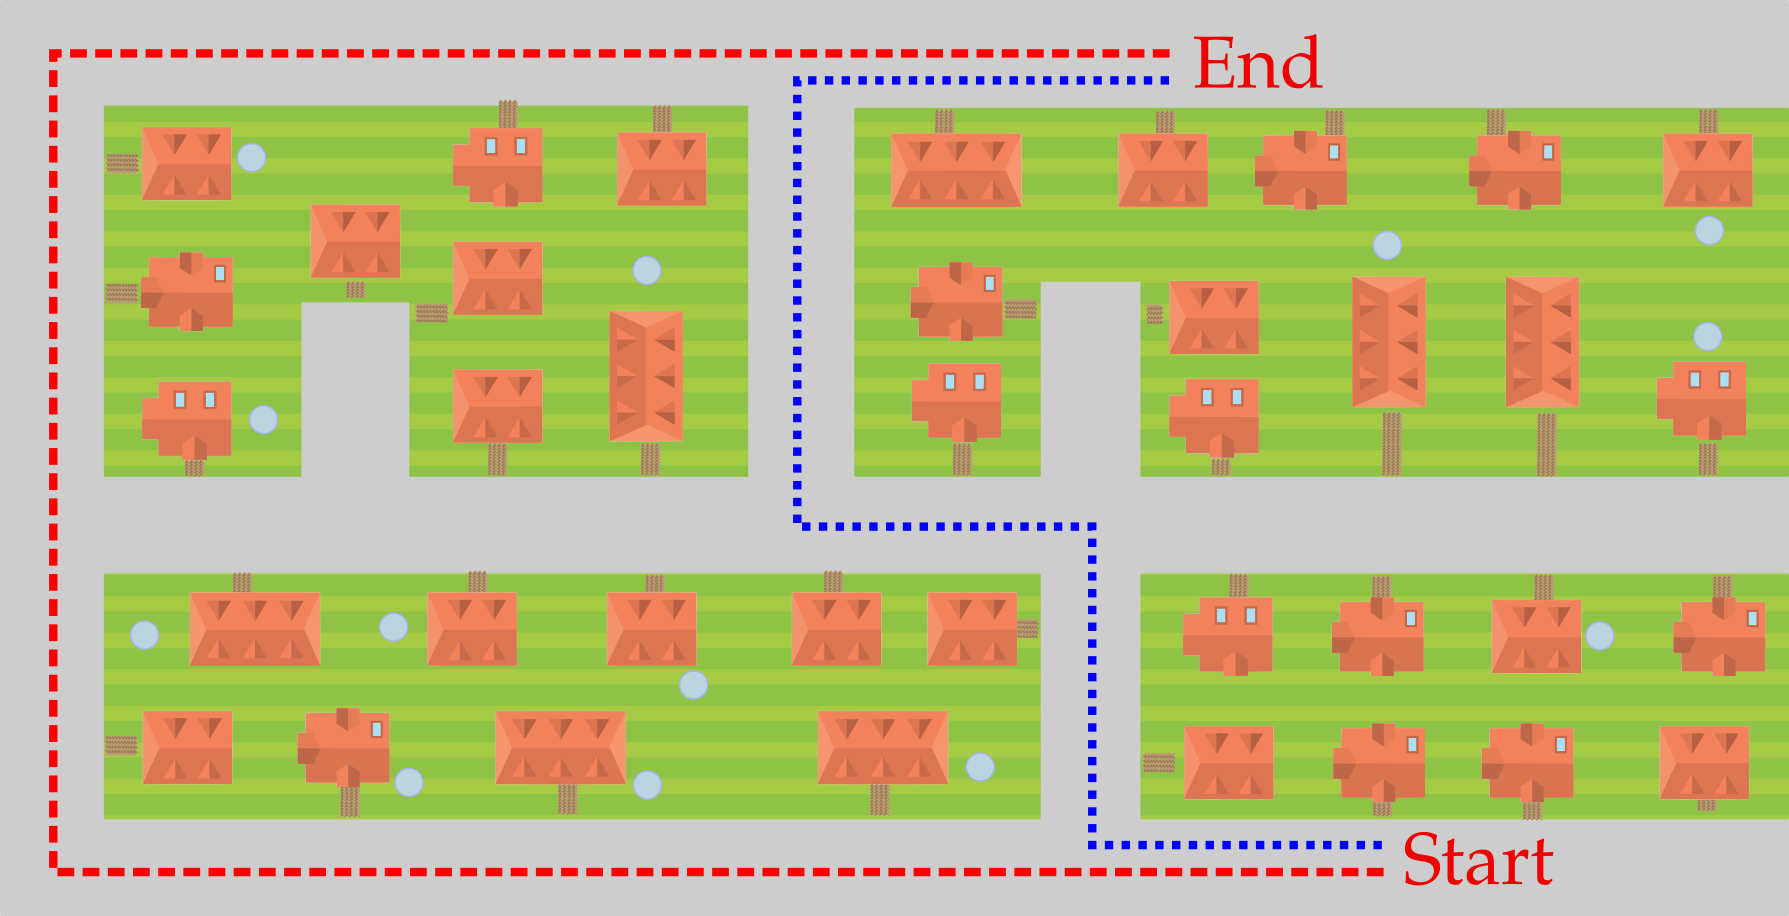
\includegraphics[scale=0.22]{figures/chapter3/landscape/landscape.png}
\caption{\label{fig:chap3_shortest} Comparison of two routes in terms of complexity and length. Even if the blue route (. . .) is the shortest many directions changing are required. Each of them is a risk for the guided person to make a mistake and be lost again. The red route (- - -), although being a bit longer, is easier to explain and to remember, and has few directions changing.}
\end{figure}

Even if the use of landmarks helps at understanding direction changing by anchoring the action to be performed, they still are a risk for the guided person to make a mistake, taking the wrong path. Where the length of the route would be an important criterion is the choice of a route, its complexity is also to be taken into account when we need to explain it. Morales in~\cite{morales_2015_building} argued that reducing the route complexity, in terms of the number of stages composing it, should be prefered to its length. This feature reduces the risk of mistake concerning the choice to make along it and also has an impact on its understanding and memorization. This criteria of minimal explanation can be compared to the Grice's Maxim of quality~\cite{grice_1975_logic}. In the example of figure~\ref{fig:chap3_shortest}, some should prefer to explain the red route rather than the blue one, even if it is longer.

Finally, to explain the same route Taylor in~\cite{taylor_1992_spatial} has noticed that a speaker can use two kinds of perspective. First, the \textit{survey} perspective trend at adopting a bird's eye view point of the environment, meaning a top view of it like as looking at a map. With this perspective, the speaker refers to the different landmarks of the route with respect to one another. They are thus referred to using terms including north-south-east-west. This perspective is opposite to the \textit{route} perspective. With such a perspective, the speaker mentally navigates along the route, making an imaginary tour of the environment. As a result, he refers to the landmarks with respect to the future guided person position along the route. The landmarks are thus referred to using terms like left, right, front, or back. In~\cite{taylor_1996_perspective}, they notice that the survey perspective is generally used for open environments whereas the route perspective is generally used in environments with already identified paths. For indoor environments, the latter should thus be preferred to facilitate route understanding and memorization.

\subsection{Environment represention to compute routes}

Regarding the environment representation generally used to find itineraries, we can first take a look to GNSS road navigation systems. In \cite{liu_1997_route} or \cite{cao_2009_gps}, we find the same principle of a topological network representing the roads with semantic information attached to each of them. Such representation seems adapted regarding the performance required for such systems operating in very large areas. However, GNSS road navigation systems must respond only to this unique task of finding a path when a robot is expected to be able to answer to various tasks. For our application, we thus need a representation that can be used more widely while still allowing the search for routes.

%Morales et al. \cite{morales_building_2015} indicate that naming parts of a geometric map does not leave the opportunity to compute such perspective. As in \cite{satake_field_2015}, we have chosen to develop our representation with an ontology as it allows to reason about the meaning of words and thus improve the understanding of human demands. In addition, we propose a way to merge the topological representation into the semantic representation (the ontology) to get the meaning of the environment elements while keeping a description of the connectivity of the elements of the environment. We propose to name it semantic spatial representation (SSR). 

% More than the extension of the spatial semantic hierarchy (SSH) \cite{kuipers_spatial_2000} allowing the representation of the environment

%This paper focuses on the presentation of the SSR and on its usability for the route description task. For now, all the ontologies used to test the SSR have been made by hand. However, many recent research work leads to automatically generate a topological representation of an environment from geometric measurements (e.g. Region Adjacency Graphs \cite{kuipers_local_2004}, Cell and Portal Graphs \cite{lefebvre_automatic_2003} or hierarchical models \cite{lorenz_hybrid_2006}, or from natural language \cite{hemachandra_learning_2014}). We have not done it yet, but our system could benefit from this work to generate a representation of an environment using SSR, which would solve the complexity of creating such a representation by hand.

\section{The Semantic Spatial Representation}

\subsection{The SSR classes}

\begin{figure}[ht!]
\centering
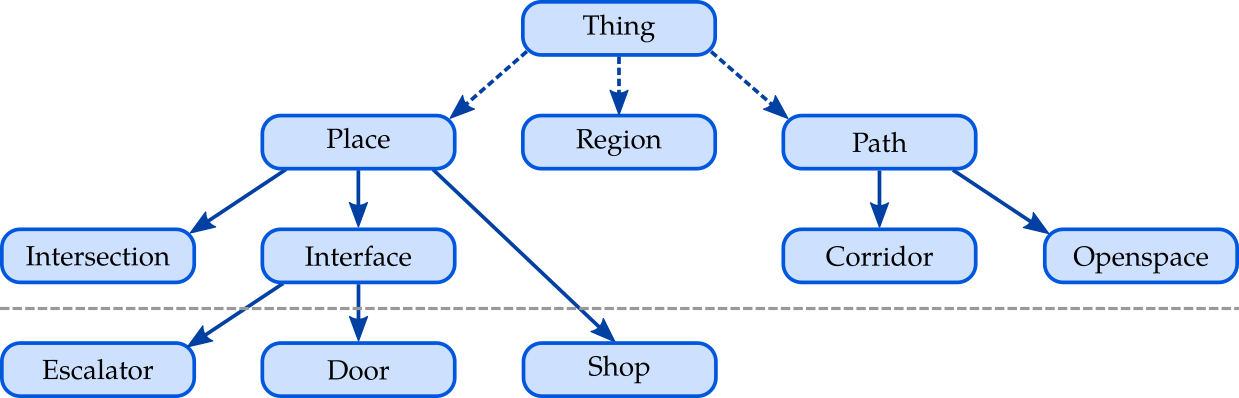
\includegraphics[scale=0.4]{figures/chapter3/ssr_tbox.png}
\caption{\label{fig:chap3_tbox} Representation fo the TBox (classes hierarchy) of the Semantic Spatial Representation used to describe the topology of an indoor environment. While the top part is inherent to the SSR, the bottom one extends the latter to provide more granularity.}
\end{figure}

\subsection{The SSR properties}

\begin{figure}[ht!]
\centering
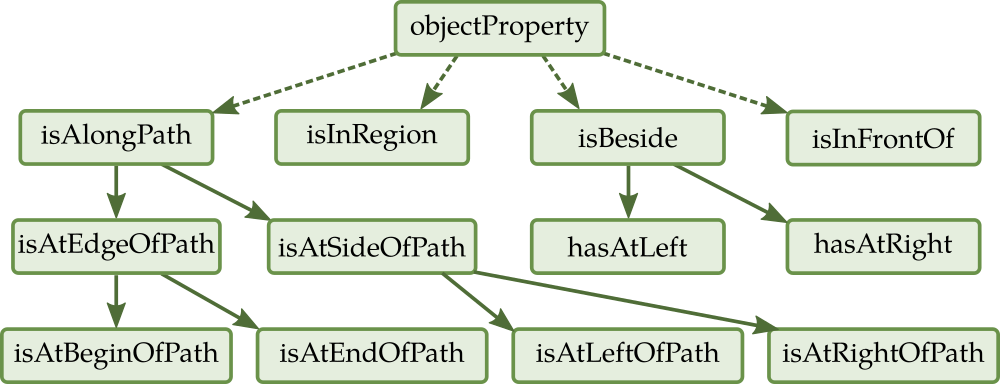
\includegraphics[scale=0.4]{figures/chapter3/ssr_rbox.png}
\caption{\label{fig:chap3_rbox} Representation fo the RBox (properties hierarchy) of the Semantic Spatial Representation used to describe the topology of an indoor environment.}
\end{figure}


\section{Finding routes to the right destination: A two-level search}

\subsection{The region-level: Trim down the search}

\begin{figure}[ht!]
\centering
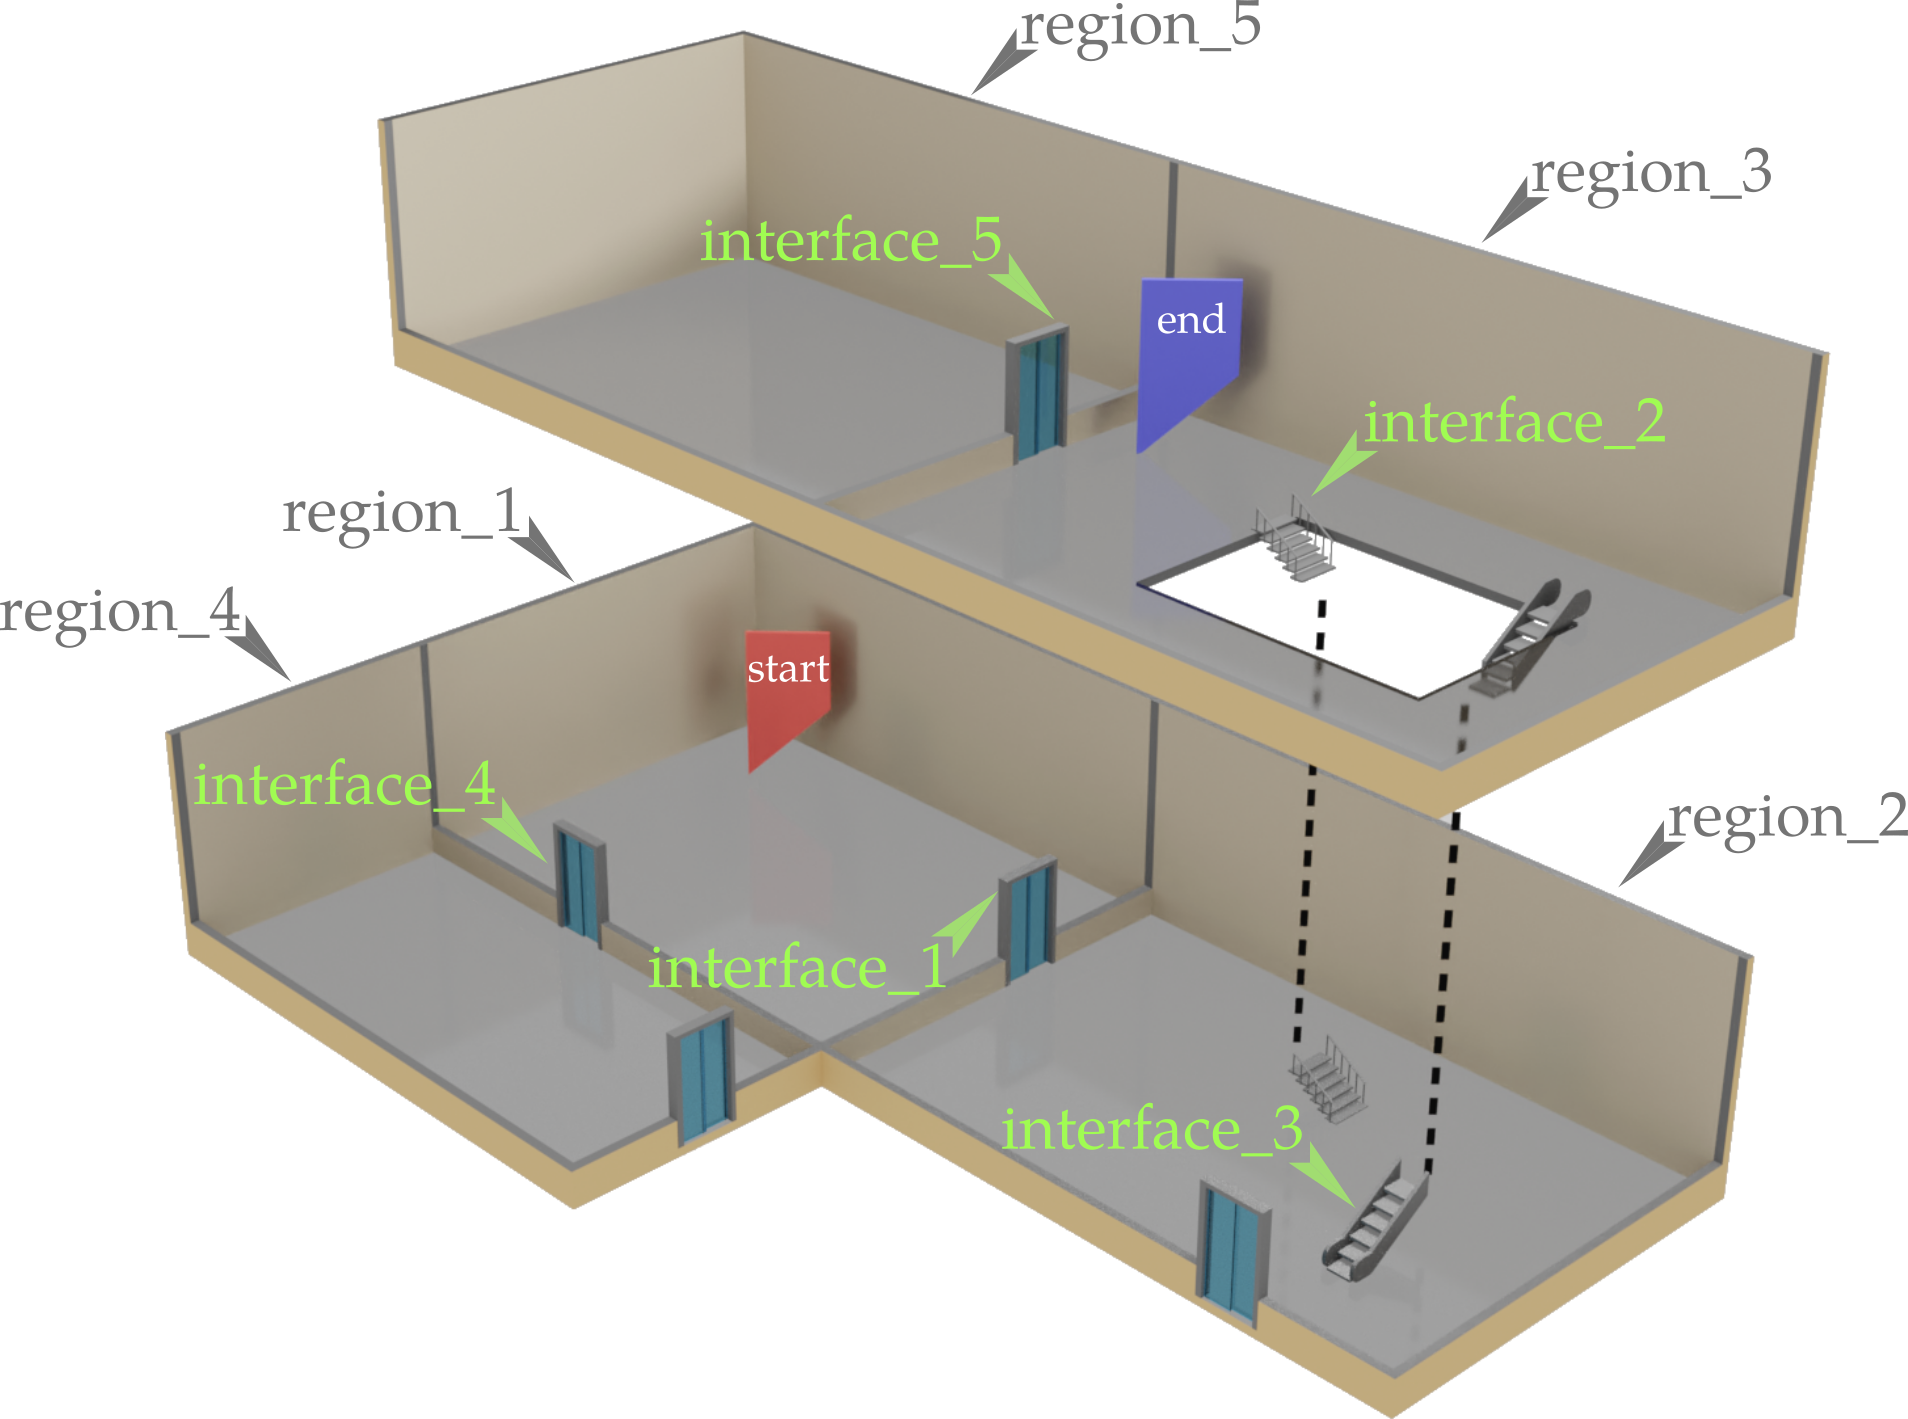
\includegraphics[scale=0.22]{figures/chapter3/building_regions.png}
\caption{\label{fig:chap3_regions} Representation of an environment at the region-level. Regions are linked trhough interfaces. We know that the starting point of the search is in \textit{region\_1} and the goal place is in \textit{region\_3}. }
\end{figure}


\subsection{The place-level: Refine the search}

\begin{figure}[ht!]
\centering
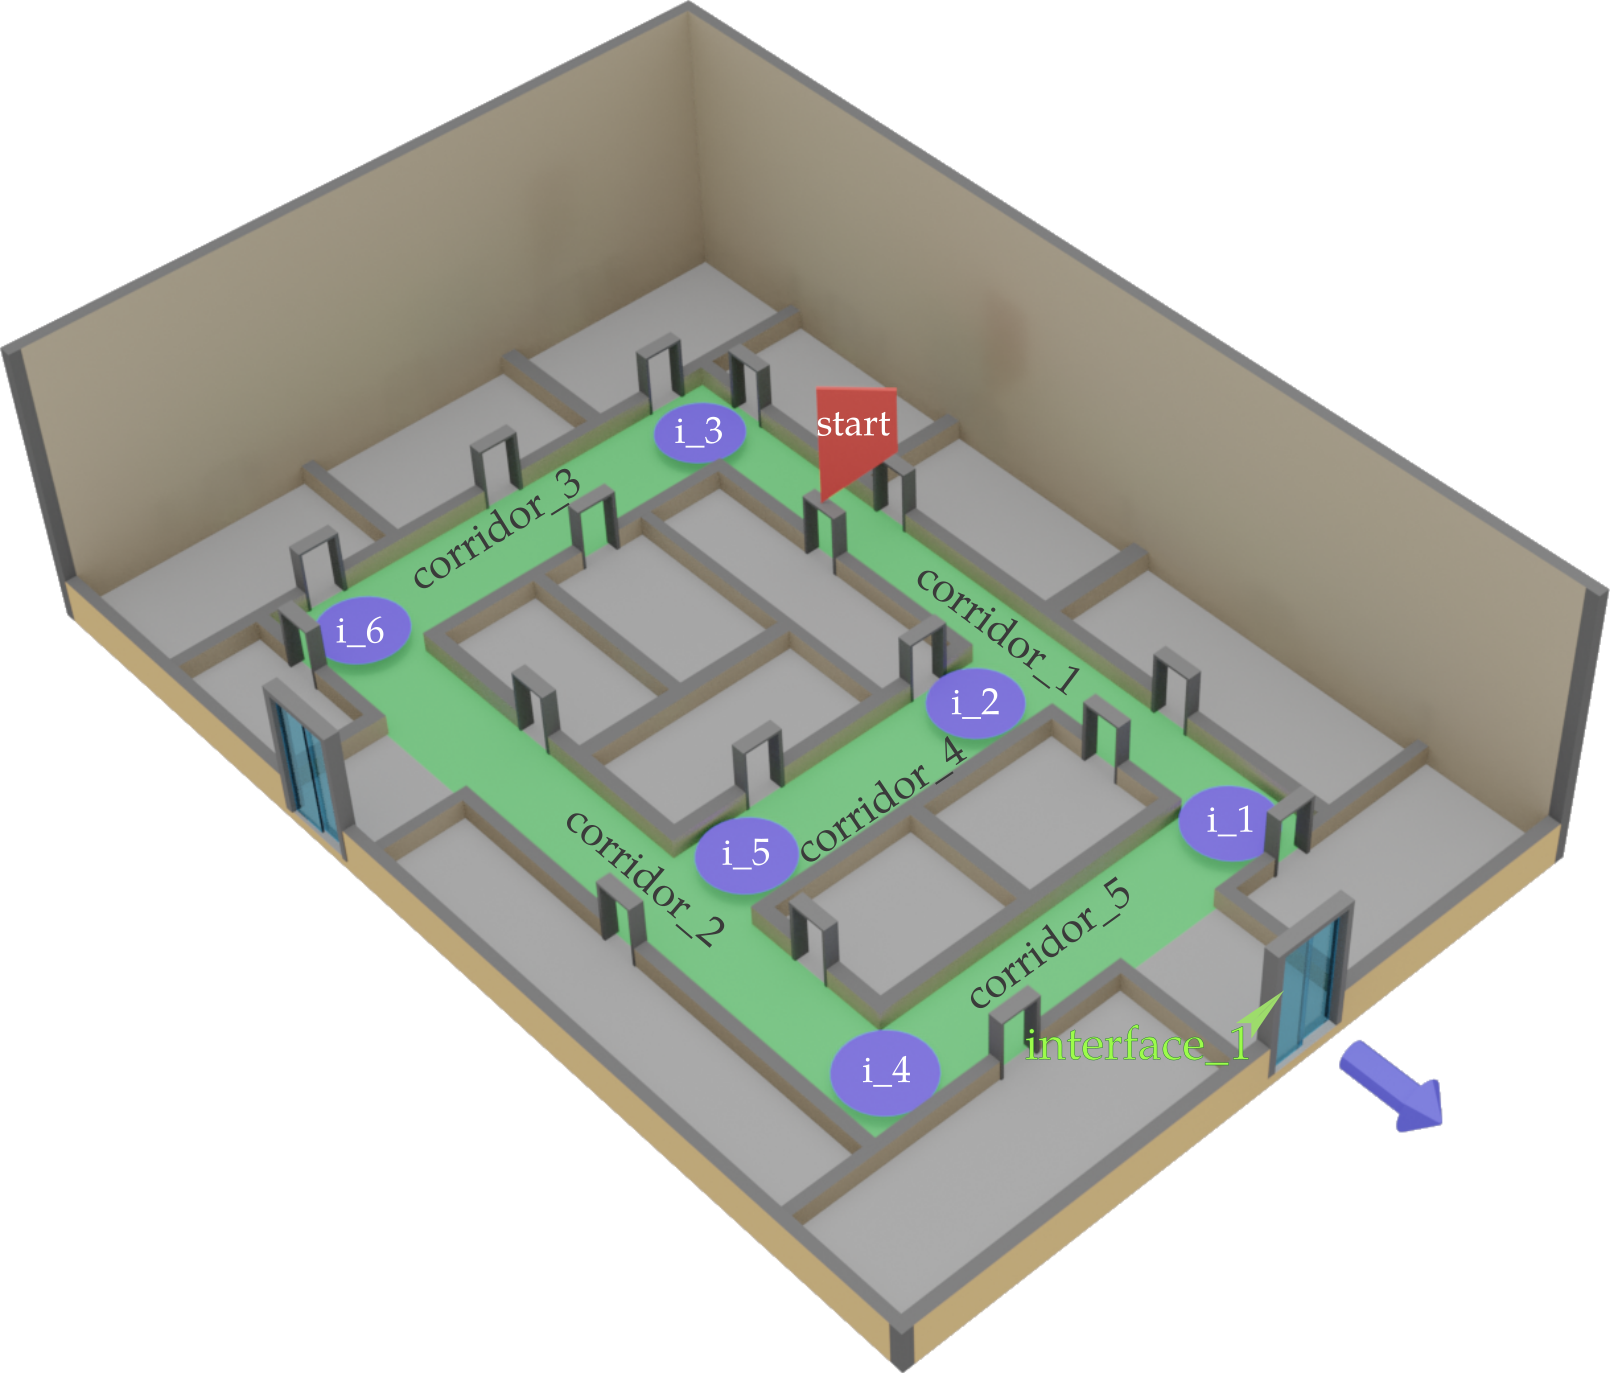
\includegraphics[scale=0.28]{figures/chapter3/region1.png}
\caption{\label{fig:chap3_region1} Representation the \textit{region\_1} at the place-level. A region is composed of paths (here corridors only) connected through intersections. We know that the starting point of the search is along \textit{corridor\_1} and the local goal place is in \textit{corridor\_5}. }
\end{figure}

\subsection{Selecting the most suitable route}

\section{Genarating an explanation in natural language}

\subsection{Putting the robot in your shoes}

\subsection{A pattern-based generation}

\section{Experiment in emulated and real environment}




\ifdefined\included
\else
\setcounter{chapter}{4} %% Numéro du chapitre précédent ;)
\dominitoc
\faketableofcontents
\fi

\chapter{Ontology-based Referring Expression Generation}
\chaptermark{Ontology-based REG}
\minitoc

The contribution presented in this chapter is excerpted from our work, published in the proceedings of the RO-MAN 2020 conference~\cite{buisan_2020_efficient}. In this manuscript, the contribution is more detailed and discussed. The presented work has been achieved in collaboration with Guilhem Buisan, with an equal contribution. Several algorithms have been developed by both of us, giving, as a result, the one presented in this chapter, merging the best of our trials. My focus was mainly on how to fully take advantage of the ontology as a knowledge base and on algorithmic optimisations to make our method the most efficient in the current literature.

\section{Introduction}

Referring to an entity is one of the most common task that we perform every day. "Can you bring me my mug? It is the black one next to the sink". "I don't remember the name of the man with the red shirt and the glasses". "I lost my keys, they are on a keychain with a soft toy in the shape of a unicorn". Such kind of communication, precise and efficient, are a key apect for the success of a collaborative tasks. Nevertheless, in complex environment with a wide variety of objects, places, or people, referring a specific entity can become a real challenge for robotic application. The robot has to take into account the context of the upper task, the diversity of facts that can be extracted from the situation and which depend on available perception modalities, and the available common ground between the robot and its partner. 

\begin{figure}[h!]
\centering
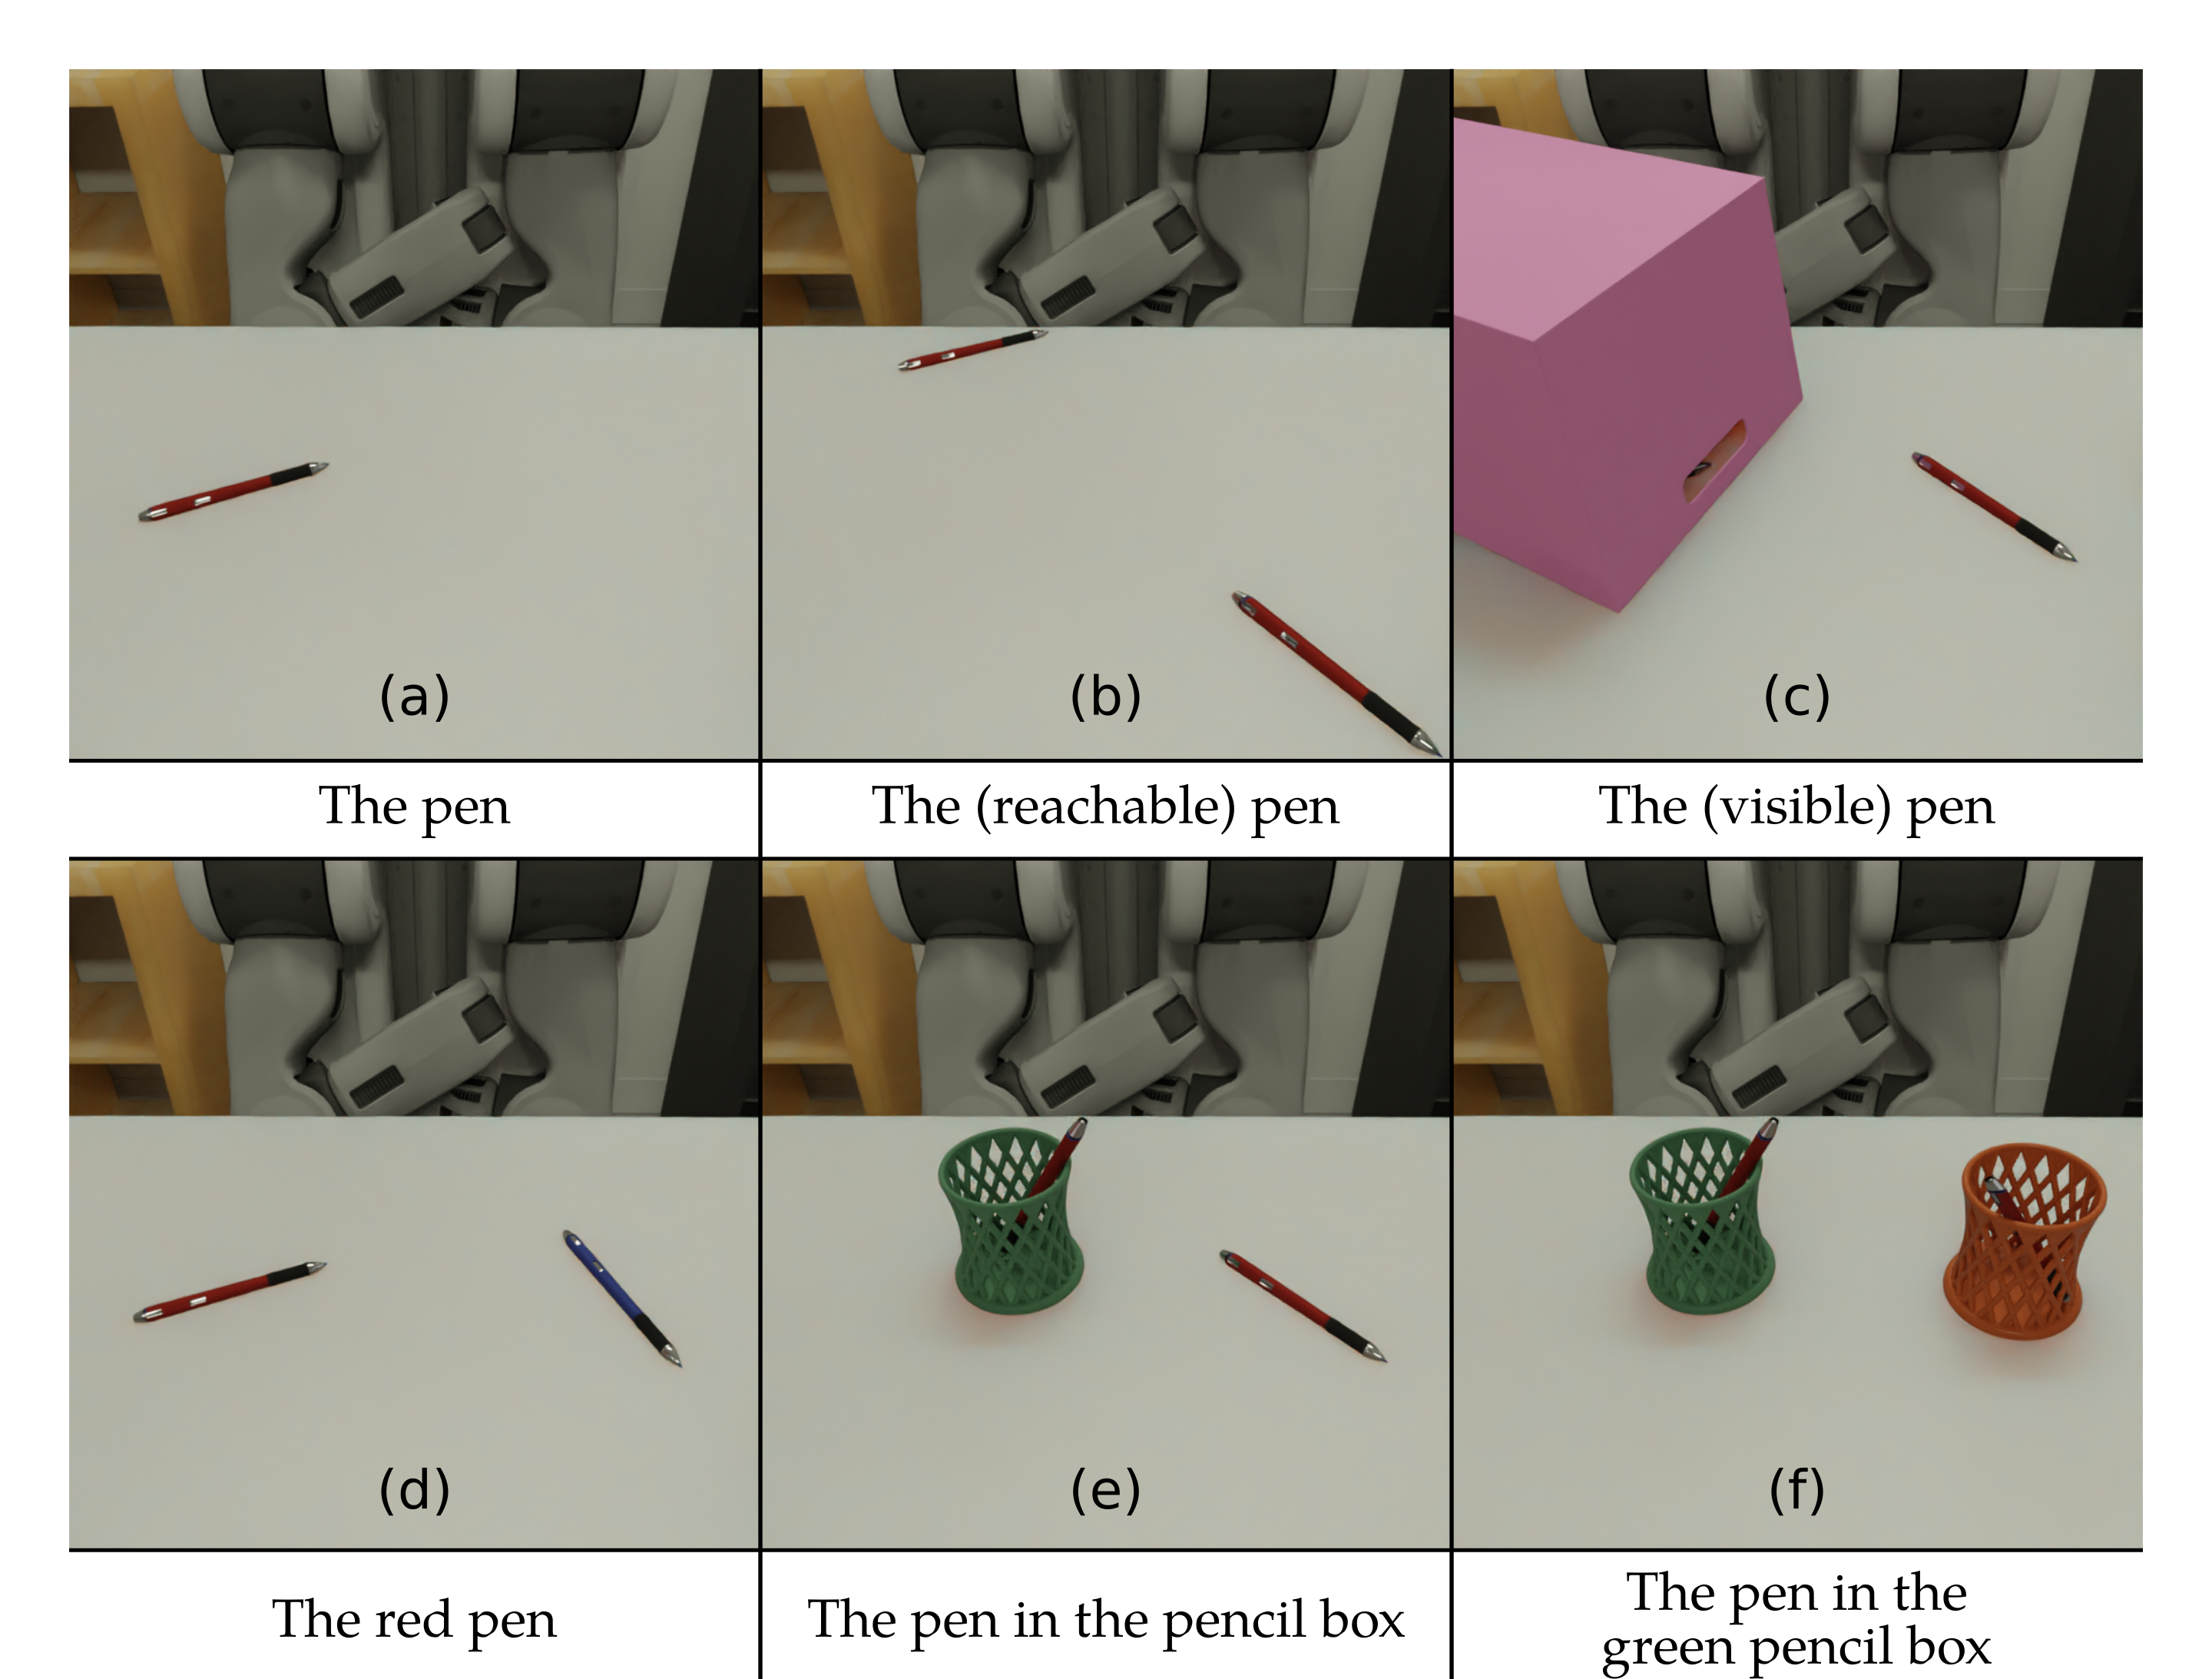
\includegraphics[scale=0.16]{figures/chapter4/intro.png}
\caption{\label{fig:chap4_intro} Six situations view from the hearer perspective, with the robot placed on the other side of the table. Referring to the same pen involves different mechanisms to raise the ambiguity, in each situation. The sentence above each situation is a possible referring expression to designate the said pen without ambiguity. }
\end{figure}

Consider the situation where you are around a table with your collaborative robot and the robot needs a pen. The simple statement \textit{"Give me the pen"} can result in several situations of different complexities. In the case where there is only one pen (Fig.\ref{fig:chap4_intro}a), the referring it is obvious. Now consider two pens on the table. If one is reachable by you (the human) and the other is not (Fig.\ref{fig:chap4_intro}b), reachability can be used to refer to the pen. If both pens are not reachable but one is visible to you and the other is not (Fig.\ref{fig:chap4_intro}c where a pen is hidden under the box), visibility through perspective-taking could be used to determine that the other pen does not lead to ambiguity. Now both pens are visible and reachable, but one is blue and the other is red (Fig.\ref{fig:chap4_intro}d). The addition of the color of the pen solves the ambiguity. If both pens have the same color but one is in a pencil box (Fig.\ref{fig:chap4_intro}e), the relation to the pencil box resolves the ambiguity. If unfortunately, both are in a pencil box but one is green and the other orange (Fig.\ref{fig:chap4_intro}f), the relation to the pencil box and the color of the latter resolves the ambiguity. We could continue like this for a long time, considering that one is at your left and one at your right, that there is no pen on the table but there is one on a shelf and so on.

Until now, we considered that the robot knows the concepts of pen and pencil box as well as their names in natural language to speak about them. However, imagine yourself travelling in another country and having to speak english\footnote{I apologize to the native English speakers who will not take full advantage of this example.}, you can sometimes miss some words and thus use more generic a one instead. However, by doing so some new ambiguity can be raised because this generic word also refers to other entities. It is the same for our robot if it has to speak French and does not know the translation of the pencil box concept. It will have to resort to a more generic term, such as "container" that can also refer to a box beside.

In addition to the concepts names, the robot must pay attention to the relationships it uses. The exact weight or length of an object wouldn't be useful as a human can not easily evaluate them. On the contrary, the color of the object seems to be a suitable property to use, unless the robot partner is color blind. This means that the robot has to use relations that it estimates to be known and observable by its partner. Such can be done considering the theory of mind and performing the generating the entity reference on the estimation by the robot of the knowledge base of the human partner.

This task to refer to a precise entity among others is commonly called the \textbf{Referring Expression Generation} (REG) task. It is often decomposed into two sub-tasks: the \textbf{content determination} and the \textbf{linguistic realisation}~\cite{krahmer_2012_computational}. The content determination aims at determining the relations to be used to refer to an entity while the linguistic realisation aims at choosing the words to be used to communicate the content. The contribution of this chapter is focused on content determination but we can not consider these two sub-tasks entirely independent. As explained earlier, if the robot does not know some concept names in natural language, the linguistic realisation will fail in the case the content determination select them or the linguistic realisation will choose a more general word that does not correspond to the determined content. We could imagine a dedicated knowledge base for the REG with only concepts usable in natural language, but such a solution is not suitable if we want a unique knowledge base for all the robotic system. Moreover, it could be hard to maintain this dedicated knowledge base during the interaction, in addition to others. 

The main contribution presented in this chapter is an \textbf{ontology-based and domain-independent algorithm for the generation of referring expressions}. It uses customizable cost function estimating the cognitive load required for a human to interpret the RE to produce \textbf{the optimal set of verbalizable assertions} that allows to refer unambiguously a given entity.

First, we review the literature concerning the REG problem and discuss the issues we aim to tackle. Then, we refine the definition of the problem to manage it at a search problem in a second part. We then compare our algorithm with two states of the art algorithms to assess its solutions and its performance. We end this chapter with integration on a real robotic system with some detail on the used perception system and the verbalization method.

\section{Related work}

Referring Expression Generation is a today classic task in Natural Language Generation \cite{gatt_2018_survey} that has been studied for decades. It has been defined by Reiter as the concern of "how we produce a description of an entity that enables the hearer to identify that entity in a given context"~\cite{reiter_2000_building}. Over time, the criteria for a good Referring Expression (RE) have been refined but still take their roots from the Grice's maxims~\cite{grice_1975_logic}. The maxim of \textit{manner} requires the communication to be unambiguous. It is also the referential success for the target entity to be unambiguously identified by the RE hearer. The maxim of \textit{relation} requires the communication to be relevant regarding the current context both the context of the task to achieve and the current world state. If you are asking someone to give you an object that is in the room where you are, you can reasonably assume that the objects in the rest of the house are not ambiguous with the one you are requesting. The maxim of \textit{quality} seems to be evident and requires the communication to be true. If you are asking a bootle and you do not know if it is full or not, you should not use this information to refer to the bottle. Finally, the maxim of \textit{quantity} requires the communication to be as informative as required but not more informative than required. In simple words, to be brief. In the context of REG, the hearer must understand quickly want you are talking about. Moreover, giving unnecessary information could lead to false implications. Saying "give me the red pen" could imply that at least one other non-red pen exists and such warn the hearer to not do the mistake to take the wrong one. If no other pen exists regarding the current context, the sentence "give me the pen" is thus sufficient.

Dale and Reiter are considered as being the pioneers of the Referring Expression Generation and have proposed over years three main algorithms solving it. Two first two fundamental approaches are the Depth First Search (DFS)~\cite{dale_1989_cooking} and the Full Brevity~\cite{dale_1992_generating}. While the first algorithm does not always find an optimal solution in terms of the number of relations used, the second does it at the cost of an exhaustive search. The most notable advance was thus the Incremental Algorithm (IA) first presented in~\cite{reiter_1992_fast} then refine in~\cite{dale_1995_computational}. With this algorithm, the notion of preference over features has been highlighted. This notion aims at representing the fact that some features are easier to understand than others. For example, the color or the shape of an object is easier the understand than spatial relations. However, the major limitation of the presented algorithms is the used knowledge representation. Because they used a set of attribute-value pairs for each entity, the solutions can only be composed of entity attributes and cannot use relations between entities. To be more precise, the algorithms can give the fact the referred entity is on a table but cannot discriminate the said table among others.

With the introduction of a new representation in the form of a labeled directed multi-graph (also known as the REG graph), Krahmer et al. solved the issue of the reference to other entities~\cite{krahmer_2003_graph}. The related Graph-Based Algorithm (GBA) REG is able to manage relations between entities and, as Dale and Reiter, consider a preference over features. This preference, called Preference Ordering (PO), is represented by a cost assigned to each edge of the graph. The GBA algorithm uses a branch\&bound algorithm which allows finding the optimal RE. On this new basis, extensions have been developed or at least discussed. Regarding the thin link with Description Logic, Krahmer raised the problem of the hierarchy of entity types in~\cite{krahmer_2012_computational}. On its side, Li et al. have proposed an optimized version of the GBA~\cite{li_2017_automatically} GBA allowing an efficiency gain close to 56\%. However, the used task only involved cubes, meaning that their algorithm does not have to take into account the entities' types, which were just added as a post-process. A last interesting GBA is the Longest First (LF) algorithm presented in~\cite{viethen_2013_graphs}. However, more than not respecting the maxim of quantity, its exhaustive search entails poor performance when used on larger realistic knowledge bases.

Learning-based approaches have of course been proposed. The belief network-based method presented in~\cite{yamakata_2004_belief} can only work with objects' attributes. Moreover, the authors indicate that a specific belief network should be constructed and therefore trained for each attribute. Such limitation reduces the genericity of the method. With a log-linear model trained from a corpus of the probability distribution of REs~\cite{fitzgerald_2013_learning}, Fitzgerald et al. face the same problem. Nevertheless, by working on belief bases, Yamakata has highlighted the importance to run the algorithm on the human partner's estimated belief base. It ensures the robot generates a referring solution compatible with concepts estimated to be known by the human.

All the algorithms presented here before are highly dependent on the task to perform. Where learning approaches are dependent on their training corpus, the other relies on knowledge bases integrating only relations usable in the context of the task. Williams et al. proposed a hybrid approach between domain-dependent and domain-independent with a distributed Incremental Algorithm (DIST-PIA)~\cite{williams_2017_referring}. The idea besides this algorithm is to make the core Incremental Algorithm independent of the knowledge representation by making it querying domain-dependent consultants~\cite{williams_2016_framework}. A consultant is an interface of a knowledge base and each knowledge base of the distributed architecture owns one. Each consultant is thus dedicated to a specific set of properties and can be query regarding these properties. To get relations about the location of entities, the Incremental Algorithm can thus query the consultant associated with the knowledge base of locations. While this solution is interesting for distributed architectures, we can ask ourselves about the domain-independence of the core Incremental Algorithm. Indeed, the ordering of the consultants to query in the algorithm can have an impact on the found solution. However, it is worth mentioning that this method has been successfully integrated into a robotic architecture~\cite{williams_2019_dempster}.

At the date, the closest work to the one presented in this chapter is introduced in~\cite{ros_2010_which}. This method uses ontology as a knowledge base. As explained earlier, such knowledge representation is suitable for domain-independent applications. However, here again, the used algorithm takes as a hypothesis that only relations useful for the REG task are present in it. Moreover, in the same way as the IA-based algorithm, their method only supports entities' attributes and not relations between entities. This method has still been integrated into a robotic system that can take advantage of perspective-taking to construct an estimated knowledge base of the human partner to give pertinent RE~\cite{lemaignan_2011_grounding}.

Even if all the presented algorithms rely on different kinds of knowledge representation and have non-equivalent abilities, they all consider a perfect linguistic realisation~\cite{krahmer_2012_computational}. We mean here that they all consider that any concept of their knowledge bases has a word in natural language and can thus be verbalize. Wanting to run on the same knowledge base as the other component of the robotic architecture, we do not want to make this assumption. Even if our contribution is focused on content determination, we aim with this contribution to make a first step in the linguistic realisation by not considering these to sub-task as being independent of one the other. We thus assume that not all the concepts in the knowledge base can be used in natural language.

To give a better overview of the progress in the REG field, the most representative contributions presented above are summarized in Table.~\ref{tab:reg_ref_sumup}. The contributions are organized chronologically and around six major features that we have mentioned throughout this section. These desired features are:
\begin{itemize}
	\item \textbf{Domain independent}: The knowledge base used by the REG must be able to be used by other components of a robotic architecture. The REG algorithm must not consider that all the knowledge represented can be used for this task.
	\item \textbf{Representation type}: The used knowledge representation must be able to be updated all along an interaction to deal with the dynamic of robotic applications.
	\item \textbf{Use of types}: The type of an entity is the minimal information to use to refer to an entity. Without type, linguistic realisation can not be done.
	\item \textbf{Preference ordering (PO)}: Some properties are easier to understand than others. Ordering the properties according to this preference allows finding efficient referring expressions.
	\item \textbf{Referring to other entities}: Entities attributes are not sufficient to find referring expressions in realistic situations. Being able to refer to an entity by referring to another one is thus mandatory.
	\item \textbf{Natural language}: Considering the linguistic realisation during the content generation could prevent the appearance of ambiguity at the linguistic realisation or even the incapacity to perform it.
\end{itemize}

\begin{table}[!h]
\centering
\caption{Summary of the most representative contributions in the REG field regarding the six major features of the problem. The contributions are listed in chronological order to give a better overview of progress in the field.}
\label{tab:reg_ref_sumup}
\begin{tabular}{lcccccc}
\hline
\multicolumn{1}{|c|}{Contributions} & \multicolumn{1}{c|}{\begin{tabular}[c]{@{}c@{}}Domain\\ inde-\\ pendent\end{tabular}} & \multicolumn{1}{c|}{\begin{tabular}[c]{@{}c@{}}Rep.\\ Type\end{tabular}} & \multicolumn{1}{c|}{\begin{tabular}[c]{@{}c@{}}Use of\\ types\end{tabular}} & \multicolumn{1}{c|}{PO}  & \multicolumn{1}{c|}{\begin{tabular}[c]{@{}c@{}}Referring\\ to other\\ entities\end{tabular}} & \multicolumn{1}{c|}{\begin{tabular}[c]{@{}c@{}}Natural\\ language\end{tabular}} \\ [0.5ex] \hline \hline
\cite{dale_1989_cooking}            & \cellcolor{red!25} No                                                                 & \begin{tabular}[c]{@{}c@{}}Knowledge\\ base entity\end{tabular}          & \cellcolor{red!25} No                                                       & \cellcolor{red!25} No    & \cellcolor{red!25} No                                                                        & \cellcolor{red!25} No                                                           \\
\cite{dale_1992_generating}         & \cellcolor{red!25} No                                                                 & -                                                                        & -                                                                           & \cellcolor{red!25} No    & \cellcolor{red!25} No                                                                        & \cellcolor{red!25} No                                                           \\
\cite{reiter_1992_fast}             & \cellcolor{red!25} No                                                                 & \begin{tabular}[c]{@{}c@{}}attribute-\\ value pairs\end{tabular}         & \cellcolor{green!25} Yes                                                    & \cellcolor{green!25} Yes & \cellcolor{red!25} No                                                                        & \cellcolor{red!25} No                                                           \\
\cite{krahmer_2003_graph}           & \cellcolor{red!25} No                                                                 & REG graph                                                                & \cellcolor{red!25} No                                                       & \cellcolor{green!25} Yes & \cellcolor{green!25} Yes                                                                     & \cellcolor{red!25} No                                                           \\
\cite{yamakata_2004_belief}         & \cellcolor{red!25} No                                                                 & \begin{tabular}[c]{@{}c@{}}Belief\\ Network\end{tabular}                 & \cellcolor{red!25} No                                                       & \cellcolor{green!25} Yes & \cellcolor{red!25} No                                                                        & \cellcolor{red!25} No                                                           \\
\cite{ros_2010_which}               & \cellcolor{orange!25} Yes                                                             & Ontology                                                                 & \cellcolor{red!25} No                                                       & \cellcolor{green!25} Yes & \cellcolor{red!25} No                                                                        & \cellcolor{red!25} No                                                           \\
\cite{viethen_2013_graphs}          & \cellcolor{red!25} No                                                                 & REG graph                                                                & \cellcolor{red!25} No                                                       & \cellcolor{green!25} Yes & \cellcolor{green!25} Yes                                                                     & \cellcolor{red!25} No                                                           \\
\cite{williams_2017_referring}      & \cellcolor{orange!25} Yes                                                             & \begin{tabular}[c]{@{}c@{}}Distributed\\ KBs\end{tabular}                & \cellcolor{red!25} No                                                       & \cellcolor{green!25} Yes & \cellcolor{red!25} No                                                                        & \cellcolor{red!25} No                                                           \\
\cite{buisan_2020_efficient}        & \cellcolor{green!25} Yes                                                              & Ontology                                                                 & \cellcolor{green!25} Yes                                                    & \cellcolor{green!25} Yes & \cellcolor{green!25} Yes                                                                     & \cellcolor{green!25} Yes                                                       
\end{tabular}
\end{table}

The literature presented here before is focused on Referring Expression Generation in its nominal form. Some researches have however addressed side problems that we do not aim to tackle. Not entering much in the details, we mention them to give a more global picture of the field. The use of spatial relations is not trivial as these relations can differ for certain entities taking the RE emitter's or receiver's point of view while for other entities, having a clear orientation system (e.g. a car), the relations remain unchanged~\cite{kelleher_2006_incremental, dos_2015_generating}. Spatial relations can also be expressed not only based on a single entity but also according to a set of entity~\cite{fang_2013_towards}. While a RE is often considered as being a single sentence referring to an entity without ambiguity, some see it as a more collaborative task where the RE is provided step by step, allowing to catch acknowledgement and to refine it according to the receiver comprehension~\cite{fang_2014_collaborative, wallbridge_2019_generating}. Finally, some research tries to integrate REG in a more global interaction where several agents refer to entities. The robot thus tries to reuse properties previously used by the partner ensuring that these properties are known~\cite{williams_2020_toward}. Limitations about this work will be discussed later in this thesis.

\section{Define the REG problem}

In this section, we present the ontology of example that we use all along with this chapter. We then discuss how the up-task in which a REG could be performed can restrict the search among the entire knowledge base. Finally, we formally define the expected form for a solution to a REG problem and the constraints it must respect.


\subsection{The knowledge representation}
\label{sec:chap4_kb}

As presented earlier in this thesis, ontology is a way to represente knowledge that is now largely used in many field becasue it allows a standardization of the representation easy extension of an extisting knowledge base, and the use of inference engine to enrich the the knowledge base. For these reasons, we choose to use a knowledge base in the form of an ontology as input of our algorithm for the REG problem. Moreover, we saw that number of recent REG algorithm have trend to use graph representations as it allows to refer to an entity through relations to other entities. Because an ontology can be see as a more complexe and mor expressive graph, this representation seems to be adequate to use for the REG problem. 

\begin{figure}[h!]
\centering
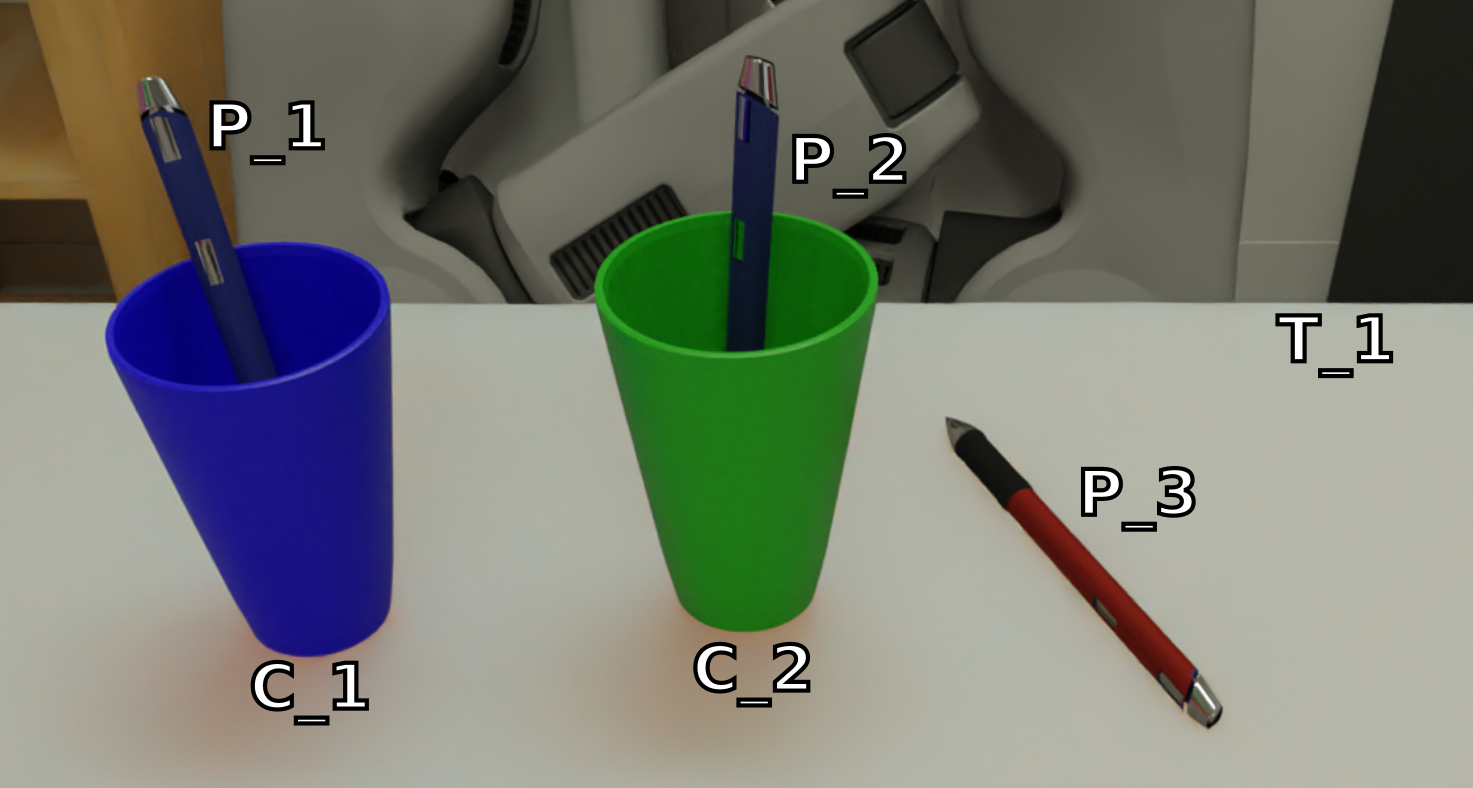
\includegraphics[scale=0.2]{figures/chapter4/pens.png}
\caption{\label{fig:chap4_kb} A situation view from the hearer perspective, with the robot placed on the other side of the table. Three pens and two cups are on a table. The two blue pens are each in one cup. }
\end{figure}

In this chapter, we take as an example the situation represented in Figure~\ref{fig:chap4_kb}. The situation is assumed to be perceived by the robot and represented in its semantic knowledge base. This knowledge base as an ontology is of the form $\kbs^R = \langle \Abox^R, \Tbox^R, \Rbox^R \rangle$. $\Abox$, $\Tbox$ like presented in Section~\ref{sec:kb_formalism}. The estimated knowledge base of the human partner $\kbs^H$ is here assumed to be the same as that of the robot in the way that $\kbs^R \equiv \kbs^H \equiv \kbs$.

The Tbox used to describe the situation of example is represented in Figure~\ref{fig:chap4_kb_Tbox}. The class IkeaLisabo represent a precise model of tables and does not have any label. The class Pen is specified through two classes the ClickingPen and the TurningPen. These two classes aim at representing the pens you need to click on top to get the tip of the pen out and the pens you need to turn to get the tip of the pen out. These classes do not have any label to directly speak about them. They are such used for the robot to know how to use them. For sure a more precise ontology could be drawn but we try to keep it simple for the purpose of this chapter.

\begin{figure}[h!]
\centering
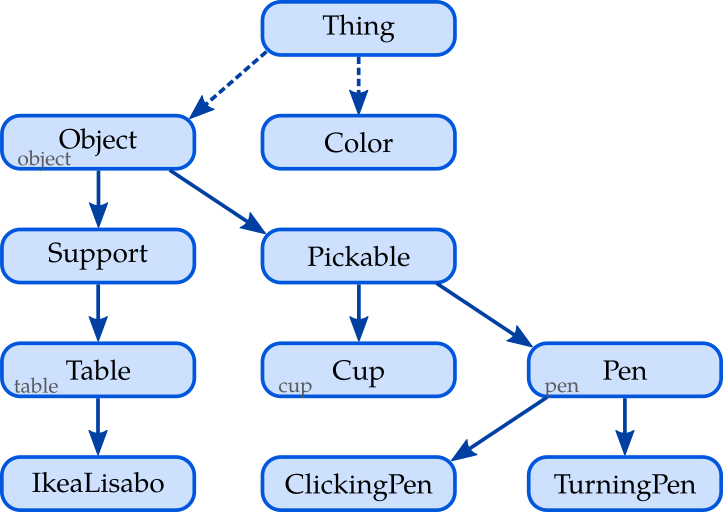
\includegraphics[scale=0.4]{figures/chapter4/pens_Tbox.png}
\caption{\label{fig:chap4_kb_Tbox} Representation of the Tbox (classes hierarchy) used to describe the situation of the Figure~\ref{fig:chap4_kb}. }
\end{figure}

The Abox used to describe the situation is represented in Figure~\ref{fig:chap4_kb_Abox}. The two cups C\_1 and C\_2 are on the table T\_1. The two pens P\_1 and P\_2 are respectivly in the cups C\_1 and C\_2 while P\_3 is directly on the table. The pen P\_4 is another pen, not on the table. Other objects could be represented as the robot and the human could know other object being in the room. the pen P\_1 is the only pen for which the agent has to click to get the tip of the pen out.

\begin{figure}[h!]
\centering
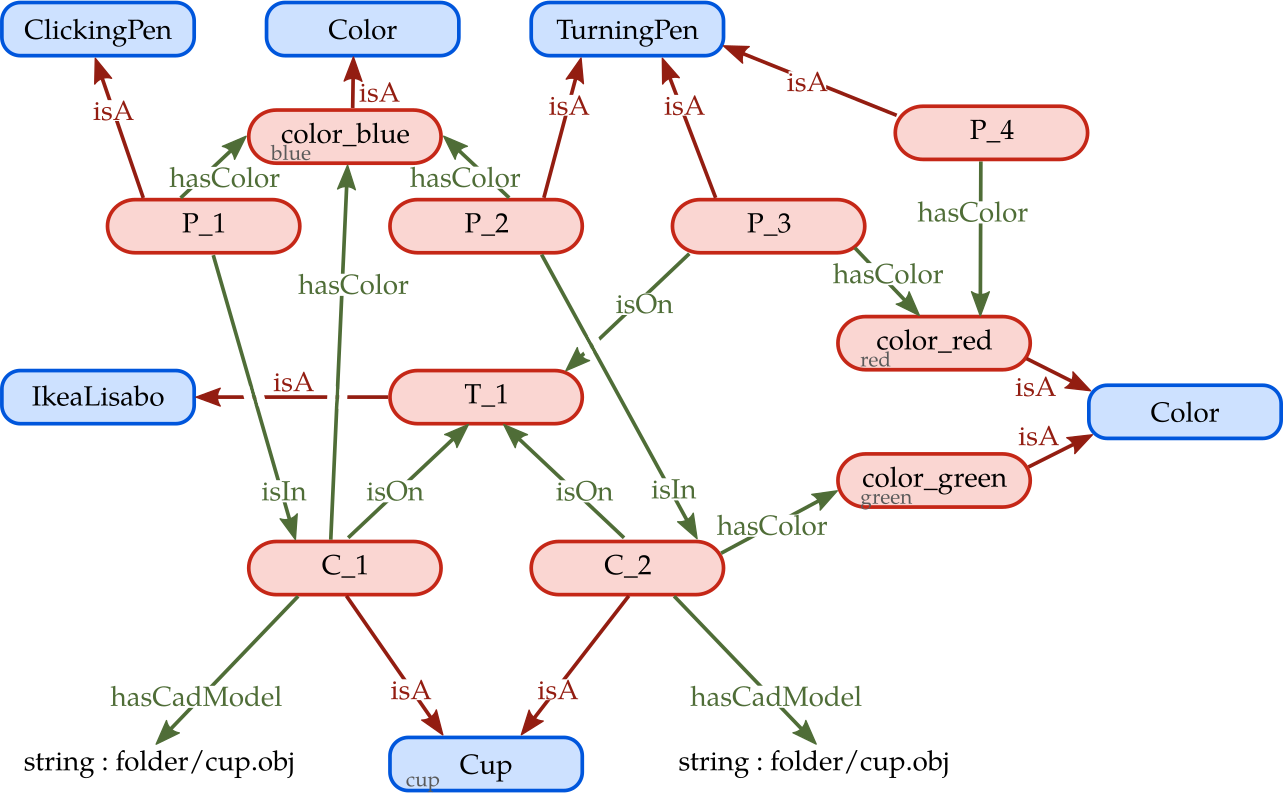
\includegraphics[scale=0.38]{figures/chapter4/pens_Abox.png}
\caption{\label{fig:chap4_kb_Abox} Representation of the Abox (relation graph) used to describe the situation of the Figure~\ref{fig:chap4_kb}. }
\end{figure}

The Rbox is not represented but the properties composing it are the ones used in the Abox. In addition with define the properties \textit{hasIn} being the inverse of \textit{isIn} and \textit{isUnder} being the inverse of \textit{isOn} ($\{(isIn,\ hasIn), (isOn,\ isUnder)\} \subset \invset$). Moreover, the property \textit{isOn} inherits of the upper property \textit{isAbove} ($\{(isOn,\ isABove), (isUnder,\ isBelow)\} \subset \inclset$). While the first state a direct contact between two entities, the other does not. Finally, we declare the chain axiom: $isIn \bullet isOn \Rightarrow isABove$. This axiom allows to reason on the ontology and declare that if an first entity is in a second one and that this second is on a third one, the first entity is above the third. Taking our example, because P\_1 is in C\_1 that is on T\_1, the pen P\_1 is above the table T\_1.


\subsection{Contextualization and restriction for situated REG}

The human (named Tony) and the robot are involved in a shared task around a table. During the task, the robot needs a blue pen to write. However, It can not take one by itself as the blue pens are on cups. Moreover, with its huge gripper, it can not use the kind of pens where you have to click. Our robot thus precisely need the pen P\_2 of our example and has to ask it to its human partner\footnote{Some could tell that if it is not the first time that our robot and this human collaborate, the human could be aware of the robot capabilities. In this case, the robot would just have to ask for a blue pen and the task would be over. We thus consider that our robot never had interacted with this particular human. For sure it could explain its capabilities but the purpose is not there.}.

The robot is thus aiming to unambiguously designate a specific entity $\goalindiv \in \indivset$, called the \textbf{target entity}, through its attributes and relations to other entities. However, as explained, the REG is meant to be used in the context of an upper task that has to be taken into account. In our example, the collaborative task concerns object on the table so that the other entities in the room are clearly out of context. Asking for a pen, P\_4 will not lead to an ambiguous situation as it is not on the table around which the interaction is performed. To represent this restriction, we provide the problem a \textbf{context} $Ctx = (\relationset_{ctx}, \inheritset_{ctx})$. It is a set of relations and direct types that are implicit in the current communication with regard to the task. This context is used to find a reference to $\goalindiv$, but has not to be included in the generated RE. For our example the context could be $Ctx = (\{ (\goalindiv,\ isAbove,\ T\_1), (\goalindiv,\ isVisibleBy,\ Tony) \},\ \emptyset)$. With this context, we state that the entity to refer to (i.e. $\goalindiv$) is known to be above the table T\_1 and visible by the human partner, Tony. Because $isAbove$ is an upper property of $isOn$, all entities on the table are concerned. Moreover, thanks to the chain axiom, any entity being in an entity on the table are also concerned. The direct types in the context could be used in a more complex communication in which we already know that we are speaking about a pen.

In addition to the entities being out of the context and thus not taken into account, some relations might be present in the knowledge base, but cannot be used in a communication process. In our example, the relations using the \textit{hasCadModel} property should not be used as the robot cannot communicate them verbally. To represent this restriction, we provide the problem a set of so-called \mbox{\textbf{usable properties}} $\usablepropset \subseteq \propset$. Any relation involving as predicate a property that is not part of the usable properties set can, therefore, not be used in the solution. Because of properties inheritance, $Incl$ all the properties inheriting from the ones in $\usablepropset$ are consequently usable to solve the problem. 


With regard to the presented restrictions, the REG problem is define as follow:

\begin{definition}[Referring Expression Generation problem]
The REG problem is a tuple $\problem = \langle \goalindiv, \kb, Ctx, \usablepropset \rangle$ with $\goalindiv \in \indivset$ the target entity, $\kbs$ the hearer semantic knowledge base, $Ctx$ the RE context, and $\usablepropset \in \propset$ the usable properties.
\end{definition}

A representation of the Abox on which the restrictions have been applied\footnote{We do not create a second Abox with the only elements that can be used. The REG algorithm will have to manage the restrictions during the search process. Otherwise, we lost the interest to run on a knowledge base common to the entire robotic architecture.} is represented in Figure~\ref{fig:chap4_kb_ctx}.

\begin{figure}[h!]
\centering
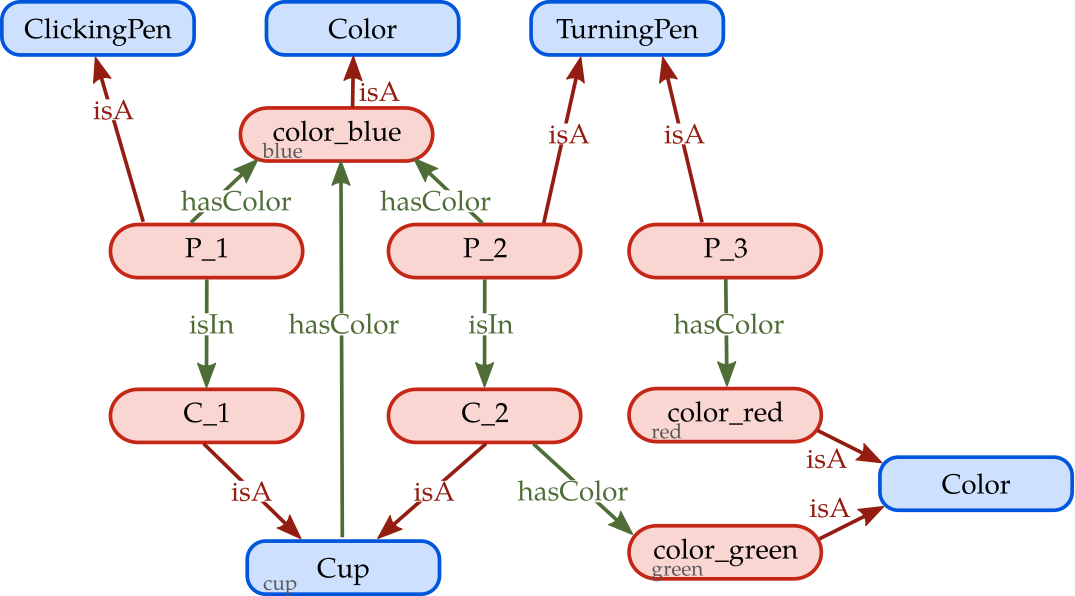
\includegraphics[scale=0.38]{figures/chapter4/pens_ctx.png}
\caption{\label{fig:chap4_kb_ctx} Representation of the Abox (relation graph) on which the context of the problem and the usable properties have been applied. }
\end{figure}

\subsection{Expected solution: structure and validity criteria}

What we could expect from a REG solver, would be a sentence in natural language. However, as explained earlier, we focus here on the sub-task that is the content generation rather than the linguistic realization. For the content generation, the attempted solution as thus often be a set of relations like $\{ (\goalindiv,\ hasColor,\ red)\}$. The issue of such a set is that it can not be verbalized afterwards. Indeed, some entities are not labelled and thus can not be used directly in the solution. They are what we called \textbf{anonymous entities}. To refer to an anonymous entity and be able to speak about it we must pass at least by its type. This is what we naturally do when we say \textit{"the red pen"} where the concept \textit{"pen"} does not directly refer to the entity by to its type. Before going ahead in the definition of the form of the solution, we can already set a constraint on its content through \textbf{the parlance need}.

\begin{theorem} [The parlance need]
\label{the:parlance_need}
For any entity appearing in a RE, exactly one naming relation must be added.
\end{theorem}

What we call a naming relation is in its simplest form the presence of a label. The relation to add is thus of the form: $(\indiv_t,\ hasLabel,\ "tony")$. In the case an entity does not have any label, we pass by one of its type which has a label: $\{(\indiv_t,\ isA,\ Pen), (Pen,\ hasLabel,\ "pen")\}$. This type is not necessarily the direct type of an entity. It could be an inherited one if needed.

Let us now introduce $\varset$, a set of variables. Because anonymous entities are not directly present in the RE sentence (hence the presence of ambiguities), we will replace all of them with variables prefixed with a question mark. The set $\varset$ thus keep a track of these variables. Taking the example of the red pen the set of relation become: \textit{\{(?0, isA, Pen), (Pen, hasLabel, "pen"), (?0, hasColor, red), (red,  hasLabel, "red")\}}. Because anonymous entities are now represented by variables, the relations representing the labels can be removed as it is implicit that the others have one. The reference is thus \textit{\{(?0, isA, Pen), (?0, hasColor, red)\}} that is exactly of the form of a \sparql{} query.

\begin{table}[b!]
\resizebox{\textwidth}{!}{%
\begin{tabular}{|l|l|l|l|l|l|}
\hline
 &
  \textbf{Target} &
  \textbf{Relations set} &
  \textbf{sparql query} &
  \textbf{Sentence} &
  \textbf{Instantiations} \\ \hline
a) &
  P\_3 &
  \begin{tabular}[c]{@{}l@{}}\{(P\_3, isA, Pen),\\ (P\_3, hasColor, red)\}\end{tabular} &
  \begin{tabular}[c]{@{}l@{}}\{(?0, isA, Pen),\\ (?0, hasColor, red)\}\end{tabular} &
  The red pen &
  {[}?0 =\textgreater P\_3{]} \\ \hline
b) &
  P\_2 &
  \begin{tabular}[c]{@{}l@{}}\{(P\_2, isA, Pen),\\ (P\_2, isIn, C\_2)\\ (C\_2, isA, Cup)\}\end{tabular} &
  \begin{tabular}[c]{@{}l@{}}\{(?0, isA, Pen),\\ (?0, isIn, ?1)\\ (?1, isA, Cup)\}\end{tabular} &
  \begin{tabular}[c]{@{}l@{}}The pen in\\ the cup\end{tabular} &
  \begin{tabular}[c]{@{}l@{}}{[}?0 =\textgreater P\_2,\\ ?1 =\textgreater C\_2{]},\\ {[}?0 =\textgreater P\_1,\\ ?1 =\textgreater C\_1{]}\end{tabular} \\ \hline
c) &
  P\_2 &
  \begin{tabular}[c]{@{}l@{}}\{(P\_2, isA, Pen),\\ (P\_2, isIn, C\_2),\\ (C\_2, isA, Cup),\\ (C\_2, hasColor, green)\}\end{tabular} &
  \begin{tabular}[c]{@{}l@{}}\{(?0, isA, Pen),\\ (?0, isIn, ?1),\\ (?1, isA, Cup),\\ (?1, hasColor, green)\}\end{tabular} &
  \begin{tabular}[c]{@{}l@{}}The pen in\\ the green cup\end{tabular} &
  \begin{tabular}[c]{@{}l@{}}{[}?0 =\textgreater P\_2,\\ ?1 =\textgreater C\_2{]}\end{tabular} \\ \hline
\end{tabular}%
}
\caption{Three referring expressions extracted from the example of Fig.~\ref{fig:chap4_intro}. For each target, is represented the relations set, the equivalent \sparql{} query, the corresponding sentence in natural language, and the possible instantiations.}
\label{tab:REs}
\end{table}

\begin{definition}[Referring expression]
A referring expression is a set of underspecified relations of the form of $(s, p, o) \in (\varset \cup \indivset) \times \propset \times (\varset \cup \indivset \cup)$ or $(s, isA, o) \in \varset \times "isA" \times \classset$ for type ascription.
\end{definition}

The form of the wanted solution would thus be as a \sparql{} query. It can easily be built from a set of relations. All the content information are present in it, in addition to the representation that some entities can not be verbalized directly. The way to resolve a \sparql{} query can be compared to the process we perform as human to understand a RE. We search all the combination of entities matching the RE. We can thus define the \textbf{correct instantiation} constraint.

\begin{theorem} [The correct instantiation]
\label{the:correct_intance}
For any variable appearing in a RE, a least one substitution function $f: \varset \rightarrow \indivset$ must exist.
\end{theorem}


Examples of REs base on the Figure~\ref{fig:chap4_intro} are presented in Tab.~\ref{tab:REs}. All three respect the constraints of theorems~\ref{the:parlance_need} and \ref{the:correct_intance}. However, the example b) does not refer in an unambiguous way the entity P\_2. We thus define the two RE validity constraints.

\begin{theorem} [The RE minimal validity]
\label{the:re_validity}
A RE is said to be minimally valid iif the variable $\var_t \in \varset$ representing the target entity $\goalindiv$ has only one possible instantiation being $\indiv_t$ itself.
\end{theorem}

\begin{theorem} [The RE complet validity]
\label{the:re_validity}
A RE is said to be completely valid iif it is minimally valid and if for all the variables $\var \in \varset$ involve in the RE, each has only one possible instantiation.
\end{theorem}

Taking the example of the Figure~\ref{fig:chap4_complet} where the goal of the situation is to refer to cup B, it can be achieved in two manners. Asking for the cup with a pen inside is a referring expression said to be minimally valid as the referred pen is ambiguous. However, not solving this ambiguity between the two pens in the cup still allow identifying the referred cup. To make the solution to be completely valid, we should ask for the cup with the red pen inside or the cup with the blue pen inside\footnote{A minimally valid reference can thus use references to set of entities. This is not an issue but the linguistic realisation should take it into account using "a" rather than "the" (e.g. "with a pen inside" rather than "with the pen inside").}.

\begin{figure}[h!]
\centering
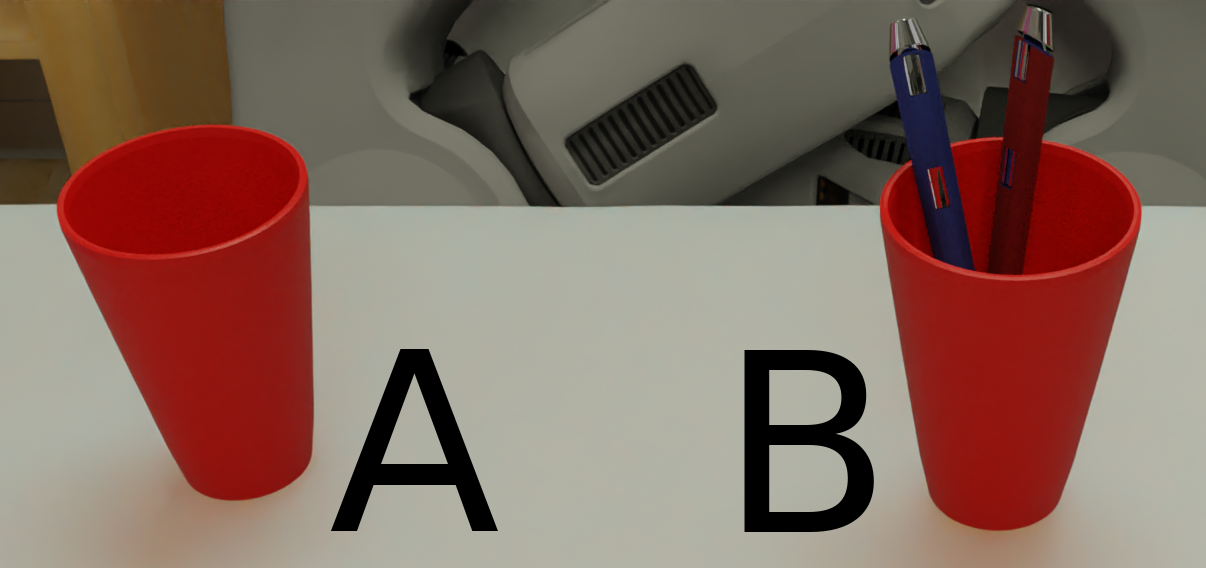
\includegraphics[scale=0.15]{figures/chapter4/complet_validity.png}
\caption{\label{fig:chap4_complet} A situation where referring to the cup B through realtions to the pens can be done either by leaving the ambiguity on the pen (minimally valid RE) or also disambiguating the color of the pen (completely valid RE). }
\end{figure}

With regard to the presentend constraints, a solution to a REG problem is define as follow:

\begin{definition}[Referring Expression Generation solution]
A solution to the REG problem is thus $\solution = \langle E, \var_t \rangle$, with $E$ a valid referring expression in the form of a set of under-specified relations representing the \sparql{} query and $\var_t$ the variable designating the target entity $\goalindiv$.
\end{definition}


Finally, considering the fact that some relations are easier to understand than others, we can define the relations cost function\footnote{The cost function is here seen as a black-box which can be a static map, the result of a learning process or other.} $\costfunc : \relationset \rightarrow \mathbb{R}^+$. Thanks to it, we can define an optimal solution to a REG problem.

\begin{definition}[Optimal Referring Expression Generation solution]
The optimal solution $\solution^* = \langle E^*, \var_t \rangle$ is thus the solution minimizing $\sum_{\relation \in E^*} \costfunc(\relation)$ over the set of all the possible solutions for a REG problem.
\end{definition}



\section{Uniform Cost Search REG}

In the previous section, we have defined a Referring Expression Generation problem as well as its solution. In this section, we first formalise this problem as a search problem and we then present an algorithm abe to solve it in a smart way.

\subsection{Formalisation as a search problem}

In the REG problem, we can consider a \textbf{candidate Referring Expression} as a \textbf{state} $\state$ of a search algorithm. A candidate RE is a RE under construction that does not respect all the constraints to make a valid RE. It is a set $\mathcal{T} \subseteq \relationset \cup C$ of relation $\relation$ representing relations present in the referenced knowledge base $\kbs$. The \textbf{initial state} is specified by the context of the problem that is a set of relations that we assume to be already known by the hearer.
%\footnote{If you do not understand why we use a set of relations while we said that a RE in s set of under-specified relations in the form of a $\sparql{}$ query, just remember that we can easily go from one to the other.}

To find all the entities referred by a candidate RE, we transform it into a \sparql{} query by replacing the anonymous entities with variables. We then submit it to the ontology to know which entities can be bound to each variable of the query. Depending on whether the result of the query gives the correct matches between variables and entities or not, we can know if a state is a \textbf{target state} or not. A state is a target state id the variables to entities matching make the RE valid (minimally or completely regarding our needs).

An \textbf{action} $\action$ in the REG problem consists in the insertion of a new triplet $(\subject, \property, \object)$ to the set $\mathcal{T}$ of a state $\state$. Performing an action on state results in the creation of a new state $\state'$. The inserted triplet can represent an entity type (coming from $\inheritset$) or a relation between entities (coming from $\relationset$). When it represents an entity type, we call the action a \textbf{typing action} with $\property \equiv isA$. When it is a relation coming from the relation set $\relationset$, we want it to reduce the existing ambiguity in a given state. we thus aim the relation to differs between ambiguous entities in $\state$. In this case, we call the action a \textbf{difference action}. To consider the open-world assumption, we can refine this difference in two categories:

\begin{definition}[Hard difference]
An hard difference exists when two entities own the same property towards a different entity: $(\indiv_i, \property, \object_i) \in \relationset \land (\indiv_j, \property, \object_j) \in \relationset | \object_i \neq \object_j$. We note this difference between two entities ($\indiv_i, \harddiff, \indiv_j$).
\end{definition}

\begin{definition}[Soft difference]
A soft difference exists when an entity owns a property that is not owned by another ambiguous entity: $(\indiv_1, \property, \object_i) \in \relationset \land (\indiv_j, \property, \cdot) \notin \relationset$. We note this difference between two entities ($\indiv_i, \softdiff, \indiv_j$).
\end{definition}

Considering the Figure.\ref{fig:chap4_complet} with the two pens, it exists a hard difference between the two pens regarding their color as one is blue and the other is red. The two pens own a relation with the same property \textit{hasColor} but on different entities, red and blue. A soft difference exists between the two cups as cup B has something inside and not cup A.

To represent the fact that some referring expressions are easier to understand than others depending on the property they use, we define a \textbf{cost} for each state. It is the sum of the cost of the properties used in the relations of the candidate RE. The cost can thus be regardless assigned to the property of the relation or the relation itself and the cost of an action is the cost of the relation it inserts. If we assume a state $\state$ with a cost $\cost$, performing an action $\action_j$ corresponds to the fact of adding a relation $\relation_j$ and create a new state $\state'$. The cost of this new state can be calculated either from the cost of the previous state $\cost' = \cost + \costfunc(\relation_j)$ or independently $\cost' = \sum_{\relation \in \mathcal{T}} \costfunc(\relation)$. In addition, as the hard differences respect the open-world assumption ut the soft differences do not, we propose to encourage the use of hard difference when possible by adding an extra cost to relations coming from soft differences.

To manage the REG problem as a search problem, we finally define a search \textbf{node} $\node$ that is, at least, composed of a candidate RE (thus a state) $\state$ and a cost $\cost$.

\subsection{Algorithm choice}

We consider the REG problem to be a graph search problem when we perform it on an ontology. If we had considered a state $\state'$ as being composed only of the relation provided by the action $\action$ from state $\state$, a tree search should have been used because state $\state'$ would depend on state $\state$. Considering a state as being a set $\mathcal{T}$ of relations $\relation$, the states become independent of each other and can be compared as $\mathcal{T}_x = \mathcal{T}_y$ iff $\forall{z},(z\in \mathcal{T}_x \Leftrightarrow z\in \mathcal{T}_y)$.

From any state, we can compute the number of pending ambiguous entities. We could think that this knowledge beyond the problem definition could be used to drive the searc. However, when we say that it still has X ambiguous individuals this means that the algorithm will have to perform at most X actions to reach a target state. This means that the heuristic function would overestimate the cost to reach the goal. In this sense, a such heuristic is not admissible and informed search is not applicable.

Although we could define the reverse actions that is to remove remations from a state, we do not know any solution of the problem and therefore we cannot do a backward search from it.

Taking a look to breath-first search, it is optimal when all steps costs are equal because it always expands the shallowest unexpanded node. However, in the REG problem, actions do not have the same cost as explained previously to represent the preference over features. In this case, the breadth-first search is not optimal and is therefore not suited to our problem.

At the difference of the breadth-first search, the \textbf{uniform-cost search} (UCS) expands the node with the lowest cost. That allows us to take advantage of the preference over features to find efficietly the optimal solution. Indeed, is \textbf{optimal} and \textbf{complete} with positive action costs and a finite number of entities and properties in $\kb$.

\subsection{Algorithm presentation}

Our REG algorithm performs a graph search in the space of states, using the Uniform-Cost Seach algorithm presented in Algorithm~\ref{alg:chap4_ucs}.
From an initial state, built from the context of the query, the algorithm generates a set of actions that add relations to the current state and create new states to explore. Just like Dijkstra's algorithm, it expands the states in increasing cost order until a solution is discovered or the search space is exhausted. We can however note a slight difference with the original algorithm. Because in our case two candidates RE said to be equivalent (i.e. owning the same relations regardless of their order) always have the same cost, we do not need to replace in the frontier a node with an equivalent state but having a higher cost than the newly created child node.

\newcommand{\tovariable}{\textsc{ToVariable}}
\newcommand{\toquery}{\textsc{ToQuery}}
\newcommand{\sparqlresult}{\textsc{SparqlResult}}
\newcommand{\createchild}{\textsc{CreateChild}}
\newcommand{\actions}{\textsc{Actions}}
\newcommand{\goaltest}{\textsc{GoalTest}}
\newcommand{\typingactions}{\textsc{TypingActions}}
\newcommand{\differenceactions}{\textsc{DifferencegActions}}

\begin{algorithm}[!htbp]
\caption{Uniform-Cost Search algorithm for Referring Expression Generation}
\label{alg:chap4_ucs}
\begin{algorithmic}
\Function{UCS\_REG}{$problem$} 
    \State $node\leftarrow$ a node with RE = \textsc{create-initial-re}(\textit{problem}.context), \textit{cost} = 0
    \State $frontier\leftarrow$ a priority queue of nodes ordered by their \textit{cost}
    \State $frontier\leftarrow$ \textsc{INSERT}($node$, $frontier$)
    \State $explored\leftarrow$ an empty set
    \\
    \Loop
        \If{\textsc{empty}($frontier$)} 
        	\State \Return failure
        \EndIf
        \\
        \State $node\leftarrow$ \textsc{pop}($frontier$)
        \If{\goaltest($problem$, \toquery($node$))} 
        	\State \Return \textsc{SOLUTION}($node$)
        \EndIf
        \\
        \State add $node.RE$ to $explored$
        \ForAll{$action$ in \actions($node$)}
            \State $child \leftarrow \createchild(node, action)$
            \If{$child.RE$ is not in $explored$ or $frontier$}
            	\State $frontier\leftarrow$ \textsc{INSERT}($child$, $frontier$)
            \EndIf
        \EndFor
    \EndLoop
\EndFunction
\end{algorithmic}
\end{algorithm}

We will now detail the functions specific to the UCS applied to the REG problem.

\textbf{\tovariable: }
We globally define a symbol table $\symboltable$ to keep track of the variables assigned to the anonymous entities. When a new anonymous entity is found, it is inserted in this symbol table with a unique variable identifier. We note $\symboltable^{-1}$ the inverse table, allowing us to retrieve the entity represented by an existing variable.

\textbf{\toquery: }
It performs the translation of a set of triplets into a \sparql{} query. To do so, anonymous entities have to be replaced by their corresponding variable. For each entity involved in the triplets to convert, they are given a string representation with the function $v(\indiv): \indivset \mapsto str$: 
\[ 
    v(\indiv) = 
    \begin{cases}
        str(\indiv),& \text{if } \alabel(\indiv) \neq \emptyset\\
        \symboltable(\indiv),& \text{otherwise}
    \end{cases} 
\]

\textbf{\sparqlresult: }
It takes a \sparql{} query as input and returns a match table $\matchtable$ in the way that $\matchtable(\var)$ is the set of entities matching the variable $\var$ in the given query. While usually the matching entities of a given variable depend on the matching entities of another one\footnote{See the example b of table~\ref{tab:REs} for an illustration of this link.}, we do not need to keep this link in our application.

\textbf{\goaltest: }
The test first fails if not all the anonymous entities involved in the tested candidate RE are typed. If this first test succeeds, the function succeeds, for a minimally valid solution, if the target entity $\goalindiv$ is the only solution to the variable $v(\goalindiv)$ in $\matchtable$. For a completely valid solution, the test succeeds if the previous test succeeds and if all the others variables of $\matchtable$ have exactly one solution.

\textbf{\createchild: } 
Creating a child node from a parent node and an action is easy to see. The \createchild function is specified in the pseudo-code of Algorithm \ref{alg:child}. 

\begin{algorithm}[H]
\caption{\label{alg:child} Child node function pseudocode}
\begin{algorithmic}
\Function{\createchild}{$action$, $parent$} 
    \State \Return a node with
    \State RE = $parent$.RE $\cup$ $action$
    \State cost = $parent$.cost + $\costfunc(action)$
\EndFunction
\end{algorithmic}
\end{algorithm}

\textbf{\actions: }
For each explored state, we consider two kinds of possible actions that we can perform on it. First, the \typingactions{} aims at proposing the addition of inheritance relations for all the anonymous entities for which no inheritance relation exists in $\mathcal{T}$. Second, the \differenceactions{}, divided into \textbf{hard difference actions} and \textbf{soft differences actions}, consists in the addition of relations that differ between the ambiguous entity for each variable in $\matchtable$.

In the \typingactions{} function (Alg.~\ref{alg:typing_action}), the function \textsc{UsableClasses} returns the most specific \textit{labeled} classes of an entity $\indiv$. In other words, it returns the set of classes $\class \in \classset$ such that $(\indiv,\class) \in C$, $\tlabel(\class) \neq \emptyset$, and
$\not\exists \class'\ s.t.\ (\class', \class) \in H \wedge \tlabel(\class') \neq \emptyset$.

\begin{algorithm}[htb!]
\caption{\label{alg:typing_action} Typing actions pseudocode}
\begin{algorithmic}

    \Function{\typingactions}{$state$} 
        
        \ForAll{$(\subject, \property, \object)$ \textbf{in} $state$}
            \If {$\alabel(\subject) = \emptyset\ \wedge \not\exists \class \text{~s.t.~} (\subject, $"isA"$,\class) \in \textit{state}$}
                \State \Return $\{\ (\subject,\text{"isA"},t)\ |\ t \in \textsc{UsableClasses}(\subject)\  \}$
            \ElsIf {$\alabel(\object) = \emptyset\ \wedge \not\exists \class \text{~s.t.~} (\object, $"isA"$,\class) \in \textit{state}$}
                \State \Return $\{\ (\object,\text{"isA"},t)\ |\ t \in \textsc{UsableClasses}(\object)\  \}$
            \EndIf
        \EndFor
        \Return OK \Comment{every anonymous entity is typed}
    \EndFunction
\end{algorithmic}
\end{algorithm}

The choice to select the most specific class differs from the one of \cite{dale_1995_computational} that prefers the least specific types also called the basic-level classes. However, using a knowledge base not specific to the REG task, it would always return the classes \textit{Object} or \textit{Thing}. This could lead to confusion for the hearer and would not help to reduce the ambiguity with other entities. Selecting the most specific thus reduce the branching factor of the algorithm as soon as possible and not impacts the completeness. Moreover, working on the estimated knowledge base of the RE hearer, we can assume that the used labels and thus concepts are known to him.

The \typingactions{} is always performed before the \differenceactions{} and this second is even not called if the first has found possible actions. We thus ensure that we do not have more than one untyped anonymous entity at the time. This particularity explains why the \typingactions{} stops at the first untyped anonymous entity. Besides, it reduces once again the branching factor. Because of the parlance need constraint, we knew that any untyped anonymous entity has to be typed to find a valid solution. It is thus useless to try to add other relation while such an entity still exists in a candidate RE. Even if, for any reason, we found ourselves in a case with multiple untyped anonymous entities at the time, each of them will be typed after the other\footnote{Typing them at once would reduce the execution time but would necessitate actions to be the insertion of a set of relations which add complexity to the algorithm for cases that should not append.}.

\begin{algorithm}[htb!]
\caption{\label{alg:diffeaction} Hard difference actions pseudocode}
\begin{algorithmic}[1]
\Function{\textsc{HardDifferenceActions}}{$state$} 
    \State $actions\leftarrow$ an empty set of actions
    \State $matches\leftarrow$ \sparqlresult(\toquery($state$))

    \ForAll{$(\var, \indiv)$ \textbf{in} matches}
        \If{$\indiv \neq \symboltable^{-1}(\var)$}
            \ForAll{$r = (\symboltable^{-1}(\var), p, o)$ \textbf{in} $\symboltable^{-1}(\var) \harddiff \indiv$} 
                \State $r_{inv}$ = $(o, Inv(p), \symboltable^{-1}(\var))$
                \If{$r \not\in state \wedge r_{inv} \not\in  state \wedge p\in U$}
                    \State $\textit{actions} \gets \textit{actions} \cup \{r\}$
                \EndIf
            \EndFor
        \EndIf
    \EndFor
    \Return $actions$
\EndFunction
\end{algorithmic}
\end{algorithm}

The \differenceactions{} function call consecutively the hard then soft differences actions functions and merge their results. The pseudo-code of the hard difference actions function is provided in Algorithm~\ref{alg:diffeaction}. The $\harddiff$ at line 6 (resp. $\softdiff$) operator returns all the relations that are hard differences (resp. soft) between two entities. In both cases, an action can be added only once and must not be present in the current state to avoid redundancy. Moreover, an action can not be added if the inverse relation to the one added is already present in the current state or proposed actions. We use the $\invset$ set defined in the knowledge base to check it. It once again avoids any redundancy. Taking the example of Figure~\ref{fig:chap4_kb}, the relation $(C\_1, isOn, T\_1)$ would be redundant if the relation $(T\_1, isUnder, C\_1)$ has been already used in the current candidate RE.

\subsection{Replanning and explaining failures}

When the hearer does not understand the referring expression, we could either repeat exactly the same sentence or be smarter and add more information than needed to help him. To do so, slight modifications have to be made to the current algorithm. In the case of replanning, the frontier and the explored set do not have to be re-initialized and in case of success, the current node has to be inserted in the explored set and the next possible actions to be found before exiting. These simple modifications are sufficient to refine a not understood RE.

When no referring expression can be found, it could be interesting to give more information about the failure to the upper process. In the case of the REG problem, it could be to give the entities still in ambiguity. With such information, an upper deliberative process could in this way act on these entities to remove the ambiguity. To do so, we just have at each step of the algorithm, to keep a track of the node having the minimum of ambiguous entities. This information is present in the matching table $\matchtable$ for each node.

\section{Results}

In this section, we present the solution found by our algorithm on the example presented in section~\ref{sec:chap4_kb}. We then challenge our algorithm on a large scale ontology representing a three-room apartment to analyse it in terms of time execution, solution length and composition. Finally, we provide comparisons with two state-of-the-art methods on their own domains.

\subsection{Solution analysis: The pen in the cup}

To familiarize with the form of the solutions and better understand how the algorithm constructs them, we first solve the example of Figure~\ref{fig:chap4_kb}. The target entity $\goalindiv$ is P\_2. The corresponding variable $\var_t$ in the \sparql{} query is denoted $?0$. We assume the general knowledge to be the Tbox of Figure~\ref{fig:chap4_kb_Tbox} and the perceived relations to be the Abox of Figure~\ref{fig:chap4_kb_Abox}.

The context of the problem is that we are speaking about objects being above the table T\_1: $Ctx = (\{(?0,\ isAbove,\ T\_1)\}, \emptyset)$. The usable properties are $\usablepropset = \{visualProp,\ geometricProp\}$. Because of the properties inclusions, the properties \textit{isIn}, \textit{hasIn}, or \textit{hasColor} are usable. The problem is thus define by $\problem = \langle P\_2, \kbs, Ctx, \usablepropset \rangle$.

Because the classes \textit{ClinkingPen} and \textit{TurningPen} do not have labels, The lowest labeled class of P\_1, P\_2, and P\_3 is \textit{Pen}. A recall of the situation and the available knowledge base on which the context and the usable properties have been applied is represented on the top of Figure~\ref{fig:chap4_search}.

\begin{figure}[h!]
\centering
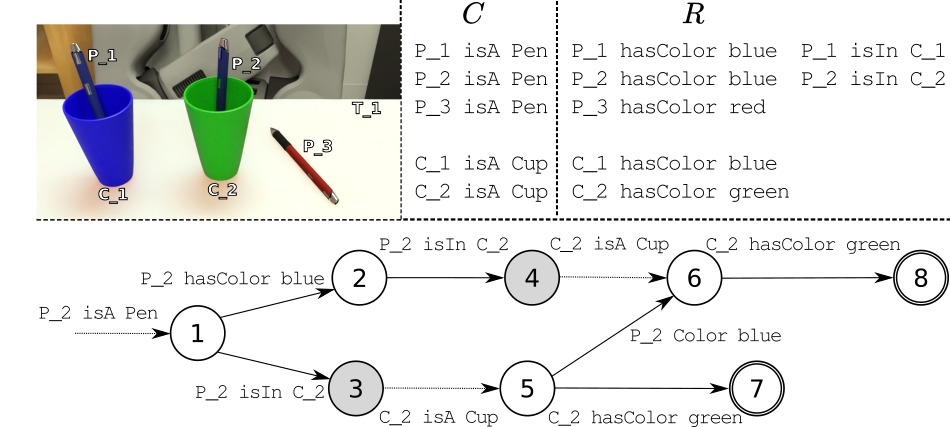
\includegraphics[scale=0.45]{figures/chapter4/search.png}
\caption{\label{fig:chap4_search} On top, a recall of the situation of Figure~\ref{fig:chap4_kb} and the entities types and relations.
At the bottom, a graphical representation of the search progress for generating a referring expression to the entity P\_2. Numbers represent the order in which the nodes are explored. Arrows are the actions performed on the nodes. Hashed arrows correspond to typing actions and greyed nodes do not respect the parlance need constraint. Double circled nodes are valid nodes. }
\end{figure}

The search process is represented at the bottom of Figure~\ref{fig:chap4_search}. It starts with node 0 in which we know that P\_2 is above the table. In this node, P\_2 is an anonymous entity and is not typed. The only possible action is thus to type it, creating node 1 with the candidate RE $\{(?0,\ isA,\ Pen)\}$. From this node, two difference actions are created and generating two new nodes. Because the action leading to node 3 introduces a new anonymous entity, it also introduces a new variable to represent it. The candidate RE related to node 3 is thus \textit{\{(?0, isA, Pen), (?0, isIn, ?1)\}}. The node with the lowest cost is explored first. In our example, all properties have a unary cost so the node to explored is selected randomly. Considering node 2 to be explored first, the entity \textit{blue} has a label so no anonymous entity has to be typed. The only possible action is that P\_2 is in the cup C\_2. Between nodes 3 and 4, node 3 has the lowest cost and is explored first. In this node, C\_2 is anonymous and not typed. The only possible action is to type C\_2. The same is done for node 4, resulting in node 6. When node 5 is explored, two difference actions are possible. However, adding the relation $(P\_2,\ hasColor,\ blue)$ to the candidate RE of node 5 results in the same state as node 6. The newly created node is thus discarded as already existing. It can also be seen as a merge of the two nodes with the same state. The second action coming from the node 5 gives the node 7 with the candidate RE \textit{\{(?0, isA, Pen), (?0, isIn, ?1), (?1, isA, Cup), (?1, hasColor, green)\}}. At this stage, the new node is just created but not evaluated. We do not know at the moment that it is a goal node. Node 6 is thus explored first and give the new node 8. Node 7 is then tested as being a goal node as the variable 0 has for only match P\_2 that is the target entity and the variable 1 can only be bound to C\_2. The algorithm does not test the node 8 has a goal node has been found.

The final solution to refer to the entity P\_2 is thus \textit{\{(?0, isA, Pen), (?0, isIn, ?1), (?1, isA, Cup), (?1, hasColor, green)\}}. It could be read as \textit{"The pen in the green cup"}. Here, we see how referring to another entity lead to interesting solutions.


\subsection{Scaling up: The three-room apartment}

\subsection{Compraritions with other state-of-the art algorithms}

\subsubsection{The longest-first}

\subsubsection{The optimized Graph Based Algorithm}

\section{Proof of concept integration on a robotic system}

\section{Integration on a robotic system}

\subsection{Verbalazing a referring expression}


\ifdefined\included
\else
\setcounter{chapter}{5} %% Numéro du chapitre précédent ;)
\dominitoc
\faketableofcontents
\fi

\chapter{Estimating communication feasibility and cost at task planning}
\chaptermark{Estimating communication at task planning}
\label{chap:5}
\minitoc

The contribution presented in this chapter is excerpted from our work, published in the proceedings of the ICSR 2020 conference~\cite{buisan_2020_human}. In this manuscript, the contribution is more detailed and discussed. In the continuity of the previous, the presented work has been achieved in collaboration with Guilhem Buisan. While his focus was on task planning, mine was on the link between the knowledge base as an ontology and the task planner. In this thesis, we will deepen this link and discuss possible improvements to the one initially presented.

\section{Introduction}

It is well established that a key aspect of the success of collaborative tasks is based on clear and fluent communication grounded in the context of the interaction. In the Natural Language Processing (NLP) research field and by extension in the Human-Robot Interaction (HRI) field, it has been divided into two dual problems~\cite{tellex_2020_robots}. On one hand, the Natural Language Understanding (NLU) aims the robot to interpret and grounds human's utterances with regard to the current situation and to react according to it~\cite{brawer_2018_situated}. In another hand, the Natural Language Generation (NLG) aims the robot to produce language. It could either be to ask for help~\cite{tellex_2014_asking}, to align knowledge~\cite{devin_2016_implemented}, or to explain its decision to its partner~\cite{roncone_2017_transparent}.

In the previous chapter, we have introduced an algorithm able to generate the content of a referring expression. Such contribution thus falls in the NLG problem. Considering the REG as an action that can be performed by the robot means that the robot could plan such communication in terms of \textbf{when} and \textbf{what} to communicate. While the "when" is directly handled by the task planner, the "what" is provided by the REG. However, the REG does not only provide the content but is also able to state if such communication is feasible or not and give information about its cost depending on the number of relations to communicate. Because the REG algorithm work on a knowledge base representing the current state of the environment, maintaining a comparable representation of the environment for the future states of the task (as it is done in symbolic task planning) would allow the robot to estimate the \textbf{feasibility} and the \textbf{cost} of the verbal communication actions all along with a task.

With these two pieces of information, a task planner could compare verbal communication with one another, compare with other means of communication, minimize the overall communication complexity, and prevent some plan failures. This approach to estimating the communication at task planning can be compared to the one proposed in~\cite{lallement_2016_symbolic}. In the latter, motion actions were evaluated at task planning to estimate their feasibility, costs, and indirect effects. With both approaches, the symbolic plans can be optimized and can be more reliable in preventing execution failures and thus the need for reparation.


\begin{figure}[t!]
\centering
\includegraphics[width=\textwidth]{figures/chapter5/intro/intro.png}
\caption{\label{fig:chap5_intro} A Human-Robot collaborative task with three colored areas and three RFID tags (situation a). The robot has to explain to its human partner to put the tag \textit{o1} in the black area and the tag \textit{o2} in the white area, to reach the situation d. The objects identifiers' are only known to the robot.
If all the communications of the task are not planned ahead, a deadlocked situation could appear if the robot first asks to move the tag \textit{o1} before \textit{o2} (situation b).}
\end{figure}

To better understand the advantage to consider the communication at task planning, consider the situations of Figure~\ref{fig:chap5_intro}. The robot has to arrange RFID tags on three areas on a table. The robot can identify them with their unique id but being too small, it can not grasp them. On the contrary, the human partner can not identify them uniquely but can grasp them. For this example, we also assume that the robot cannot point to the tags. The robot must therefore communicate the successive actions that the human will have to perform to go from the inial configuration (\ref{fig:chap5_intro} a) to the goal configuration (\ref{fig:chap5_intro} d). Between both configurations, only the tags \textit{o1} and \textit{o2} have to be moved. The tag \textit{o1} has to be move from the red area to the black and \textit{o2} from the black area to the white. While the tag \textit{o3} can be referred to unambiguously thanks to its color, the two others can not. However, they can be referred thanks to the area they are in (e.g. \textit{"the tag is the red area"}).

If the content of the communications is only refined at execution, two equivalent solutions can be planned (\ref{fig:chap5_intro} sequence a-b-d and a-c-d). At execution, the first solution begins by asking the human to move \textit{o1} in the black area resulting in the instruction \textit{"take the tag that is in the red area and put it in the black area"}. In this new situation where both red tags are now in the black area (Figure~\ref{fig:chap5_intro}b). The robot has no way to designate the tag \textit{o2} without ambiguity. Hence, the task is blocked\footnote{The robot could use spatial relation like right, left, or the closest to me. However, the generation of such RE is not an easy job and the understanding of it neither. Even if the situation is not really blocked, the required communication can be complex. }. Estimating the communication feasibility and cost during the planning process would result in the second possible solution. The robot first ask to move the tag \textit{o2} (Fig.~\ref{fig:chap5_intro} c) and then the tag \textit{o1} (Fig.~\ref{fig:chap5_intro} d). If the robot could have pointed, the deadlock of the first solution can be avoided with a pointing action and nevertheless, thanks to the communication cost estimation, the least expensive solution can be selected\footnote{Plenty of other solution could exist but depend on the robot capability. Giving the two instructions in the initial state before the human act solve also the problem for example. Nevertheless, if the robot cannot compare these different solutions regarding its current capability, non-desirable situations could still appear.}.

The main contribution presented in this chapter is an approach to \textbf{estimate the communication feasibility and cost at task planning}. It implies a fine \textbf{link between a planner and an ontology} to estimate communication grounding in the future estimated state of the environment.

First, we briefly review the literature concerning the task planning problem and discuss the issues we aim to tackle. Then we, give an overview of the involved components with a focus on the task planner while the others have been detailed in the previous chapters. We then present how the fine integration of the components allows us to take estimation the communication at task planning and discuss possible improvement. We end this chapter with three case studies, to show how this approach can be used to prevent deadlocked situations at execution, how it can reduce the global communication complexity during a Human-Robot collaborative task and how it can be used to balance between different communication means.

\section[Related work]{Related work: The need to plan communication}

A significant amount of research has been dedicated to Human-Robot verbal communication, especially to answer the questions of \textit{what} and \textit{when} to communicate~\cite{mavridis_2015_review}. A lot of early works address these questions at execution time, with a fixed plan in which the robot inserts verbal communication afterwards when needed. The communication can be used to share and negotiate plans~\cite{sebastiani_2017_dealing}, to ask for or give specific information~\cite{shah_2011_improved}, to repare errors~\cite{tellex_2014_asking}, align knowledge~\cite{devin_2016_implemented}, or increase trust~\cite{schaefer_2017_communicating}

In their work~\cite{devin_2016_implemented}, Devin and Alami the robot is provided with a shared plan for both itself and its human partner. On top of that, they use a theory-of-mind enabled framework to estimate throughout the interaction the partner's mental state about the current state of the environment and the performed actions. When the robot perform an action while its partner performs another one in a different room, the robot can detect a belief divergence due to the fact that the partner can not know if the robot has acted or not\footnote{This is the case when the action performed by the robot has no perceptible effects on the environment like scanning object.}. When such divergence is detected, if it can endanger the overall plan, leading the human to perform a wrong action, or block the interaction, if the human wait for an action already performed by the robot, verbal communication can be inserted at execution time. The content of the communication is determined with regard to the divergences that can break the shared task.

However, in most cases, deciding communication at execution time is not enough and more recent works deal with communication actions at the planning level. Nikolaidis et al.~\cite{nikolaidis_2018_planning} identify two types of communication: \textit{commands}, where the robot ask for an action to be performed by its partner and \textit{state-conveying} to inform about its internal state. They use a Mixed Observability Markov Decision Processes (MOMDP) to determine the need for communication and its type, returning a policy capturing the probability of the human to take a given action based on the performed communication. A comparable approach is presented by Roncone et al.~\cite{roncone_2017_transparent} with three types of verbal communication action: \textit{command} to instruction to the human to perform an action, \textit{ask} to be informed if the human current action is over, and \textit{inform} to communicate an intent. These communications are integrated with others actions into a Partially Observable Markov Decision Process (POMDP) which returns a policy integrating communication actions. However, for both presented approaches, the communication complexity and thus costs are not taken into account. Moreover, while for the first the content is pre-generated, for the second it is not specified at the planning level. This can cause non-achievable communication in some situations.

A similar approach is proposed by Unhelkar et al. \cite{unhelkar_2020_decision} with more communication types considered: \textit{command}, \textit{ask}, \textit{inform} and \textit{answer}. This time, a communication cost is explicitly considered. However, the cost is related to the \textit{when} to communicate and not on the \textit{what}. It is represented by a function penalizing temporally close communication actions. Concerning the content, is is patterns including parameters replaced at execution time. For example, in the sentence \textit{“Please make the next sandwich at -landmark-.”} the sentence representing landmark will be resolved at execution. In their examples, every landmark is assumed to be easily referred to the human, but this is not always the case. Using the REG at task planning, our approach addresses two of the five challenges identified by Unhelkar et al.: "estimating benefit of communication" and "quantifying cost of communication"~\cite{unhelkar_2017_challenges}.

\begin{figure}[!ht]
\centering
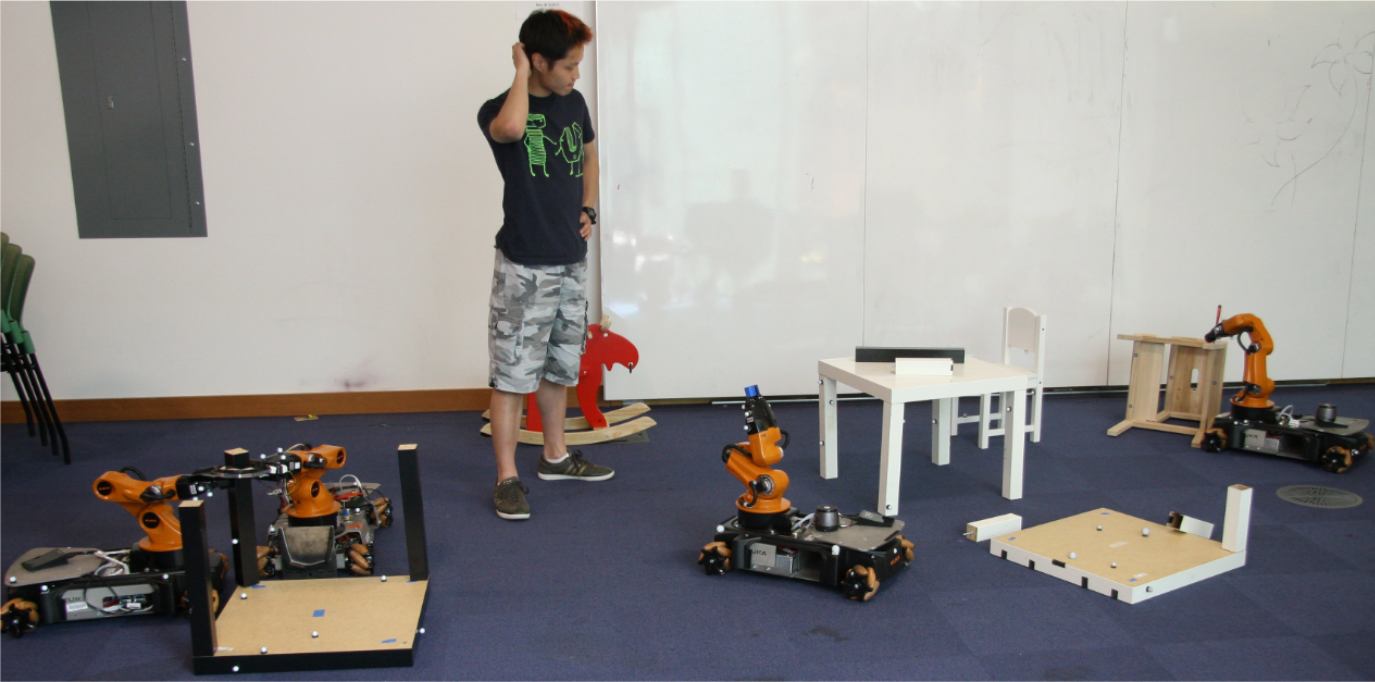
\includegraphics[scale=0.25]{figures/chapter5/tellex.png}
\caption{\label{fig:chap5_tellex} Illustration from \cite{tellex_2014_asking}.
A robot engaged in assembling a table requests help using natural language with targeted requests such as “Please hand me the white table leg." }
\end{figure}

To better understand the difference of our approach regarding existing work, we use the example depicted by Tellex et al. \cite{tellex_2014_asking} and illustrated in Figure~\ref{fig:chap5_tellex}. In this situation robots, following a precomputed plan, are assembling furniture. During the task, the robot assembling the white table encounter a failure because it can not reach the needed table leg (on the other white table). When such a failure occurs, the robot asks a human for help by referring to the object at the origin of the failure. By doing so, the robot performs a plan reparation with the help of the human and thanks to an object referring communication action. However, if the leg has not been move since the beginning of the task, the non-reachability of the leg could be known by the robot during the planning process. The non-reachability is not really of failure and such reparation could be avoided. Considering the task as a shared task, the assembly of the leg could be assigned to the human. Keeping the human in the role of a helper, verbal communication still could be planned either to group multiple communication reducing the human disturbance, or to perform it in order to make the communication easier. The robot would have assembly the other white leg to only refer to the last one as "the white leg" not leading to any ambiguity with the other ones.


\section{The involved components}

The type of communication actions we want to manage in this chapter is commands using Referring Expression presented in the previous chapter. Typical commands will be composed of a static part and situation-dependent one like \textit{"Take X"}, \textit{"Put it in Y"}, or \textit{"Take X and put it in Y"}. The variable part depends on the state of the situation when the communication is performed and must be solved by a REG. The communication feasibility and cost thus depend on this variable part and by extension of the moment where it is used.

As explained previously, the REG aims to be run on the human partner estimated knowledge base to ensure that all the concepts and relations used in the generated RE are known to him. To be able to estimate communication about the future states of the environment and keeping this principle to run on the estimated KB, we need a symbolic task planner already suitable for HRI. It has to able to distinguish between the different agents involved in the task and to maintain an independent representation of the environment for each of them.

To resolve a specific task, a planner does not necessarily need to be aware of all the elements present in the current environment. It simply needs a representation of the entity that can be used to solve the task. To solve the task of assembling a table, it only needs the table elements for this particular one even if others a present in the environment. Even if we could represent all the elements, it would be counterproductive by not helping to solve the task but adding exploration complexity.
In the same way, it does not need a fine representation of these elements. Even if the task is to create a cube tower with alternating colors, the color information is not necessarily useful. In the introduction example (figure~\ref{fig:chap5_intro}) the color of the RFID tags does not matter for the task and the type of the objects are also useless. Representing them as movable objects\footnote{To not move the areas around the tags instead of moving the tags.} could be sufficient. Moreover, doing so make the planner more generic as not being restricted to arrange RFID tags. However, we saw that for the REG, the more the situation will be described precisely (both in term of types and relation), the more accurate the solution will be. Furthermore, if another tag, which is not part of the task and thus not part of the planner internal representation, is present on the table, it will also impact the REG and thus the complexity and feasibility of the communication action. 

This difference of representation requirement between the task planner and the REG lead to the fact that the REG can not be performed on the planner internal representation. To solve this issue, we have to endow the planner with the ability to maintain a semantic KB that is used by the REG. Before going further in the way to solve this challenge, we will first present the newly introduced components being the task planner. WE then give more detail about the knowledge base we will consider for this application.


\subsection{The Hierarchical Task Planner}

To implement our approach, we just see that we need a task planner able to maintain an independent estimated knowledge base for each agent involved in the task. We chose the Hierarchical Agent-based Task Planner (HATP\footnote{Also called Human-Aware Task Planner})~\cite{lallement_2014_hatp}. HATP extends the classical Hierarchical Task Network (HTN) planning by being able to produce \textbf{shared plans} to reach a joint goal. A HATP planning domain describes how to decompose tasks into subtasks down to atomic symbolic actions. Both the robot and human feasible tasks and actions are described in the domain. A context-dependent cost function is associated with each action. 

During the task decomposition, HATP will explore several applicable sub-tasks until the global task is totally refined into feasible actions, and will return the minimal cost plan. HATP also supports \textit{social rules}, allowing to balance the effort of involved agents depending on human preferences and to penalize plans presenting certain undesirable sequences of actions. We will not use these social rules in what follows, but our approach stays compatible with them.

Moreover, during the exploration of the task tree, HATP will assign actions to available agents, robot or human (when an action can be done by both). By doing so, HATP can elaborate one \textbf{action stream} per agent, together with causality and synchronization links. 
Besides, HATP domain syntax supports Multiple Values State Variables (MVSV)~\cite{guitton_2012_belief} which is used to represent and reason about each agent mental state. The value of each variable depends on the agent it is requested for. This allows representing action preconditions depending on the knowledge of the agent performing the action and also represent their effect on each agent mental state which can depend on the agent perspective.

Finally, the last argument which motivated our choice was the use of HATP in previous work: the Geometrical Task Planning (GTP) \cite{gharbi_2015_combining}. This work aimed at refining into motion planning requests the symbolic motion actions explored by HATP during the task planning process. The motion planner would then returns the feasibility and the cost of the action, but was also able to inform HATP about why the motion action would not be possible (e.g. the object with which collision would occur). The task planner would then, backtrack to choose a different action to remove the colliding object. This method also shows how to update the geometrically planned environment to math the symbolic one to run the motion planning phase. This approach also needs to update the geometrical planned world to match the symbolic planned knowledge base before running the motion planning phase. This work greatly inspired us, and our approach is similar at the difference that we run a REG when a communication action is explored, instead of a motion planning request on a symbolic motion task exploration.

\subsection{The semantic knowledge base}

In the previous applications of this thesis, we could use only one knowledge base representing both the robot's and human's knowledge about the environment. This time, because the task planner explicitly manages an independent world state for each agent, we will fully take advantage of Ontologenius to manage several ontology instances at the time. We will thus note the robot's semantic knowledge base $\kbs^R$ and, considering only one partner, the human estimated knowledge base $\kbs^H$. Both will be kept up to date at the same time. This means that both represent the knowledge of each agent at the current time. However, as explained in the introduction of this section, we need to run the REG on a knowledge base that will represent what the robot believes that its partner will know about the future states of the environment. In other words, take the initial state of the introduction example of Figure~\ref{fig:chap5_intro}. If the robot plan to remove the tag \textit{o1} from the table and want to estimate the feasibility of referring the tag \textit{o2} if the first action is performed, it has to remove \textit{o1} from the table in the estimated knowledge base of the human to evaluate this future communication. Nevertheless, it can not modify $\kbs^H$ as it represents the current estimated knowledge of its partner. Performing such modification could have side effects on the entire robotic architecture. To deal with that we will use the Ontologenius feature that consists of the copy of an existing ontology instance. For remember, a copied instance then become independent from the original ontology. The instances representing a future possible mental state of a human will be noted $\kbs^{H_i}$. In this way, the REG can run on a $\kbs^{H_i}$ for the planning process and on $\kbs^H$ at execution.

\section[Integrating planners]{Integrating task and communication planners}

The general scheme of our approach to enabling a symbolic task planner to estimate the feasibility and cost of future communication is the one presented in Figure~\ref{fig:chap5_integration}. On the top of the figure, we have large, complete semantic knowledge bases representing the robot knowledge and the other agents estimated knowledge. At the bottom of the figure, we have the planning process with reduced knowledge bases dedicated to task planning. As explained earlier, because the planning process will need to represent the future estimate mental state of its partner without altering the original estimation, we first perform a copy of the human estimated ontology. From there, it because an independent knowledge base capturing the human knowledge about the environment at a given instant. We call this new ontology the human planned ontology and denote it $\kbs^{H_0}$. At the initialization of the planning process, once the copy performed, the planner extract from the robot ontology and the human planned ontology the symbolic facts it needs. To do so, every entity types declared in the planning domain are retrieved from the ontologies by their name, and entities inheriting from these types in the ontologies are created in the planning knowledge base. Then, each attribute (both static and dynamic) of every entities declared in the domain has its value updated. If the attribute is a set, multiple relations with the same name originating from the same entity and pointing to different ones can be found in the ontologies. If so, all the pointed entities are added to the set.

During the task network decomposition, the general workflow executed for each communication action encountered consists of 1) updating the human planned ontology with the expected world state 2) identifying the objects involved in the communication 3) execute the REG for each of these objects 4) calculate the feasibility and the cost of the communication action according to the feasibility and the cost of each individual RE involved in the planned communication. Note that if multiple objects have to be referred to in single communication (e.g. \textit{"give me X and Y"}), the human planned ontology is only updated once as the estimated state in the same bor both REG.

\begin{figure}[!ht]
\centering
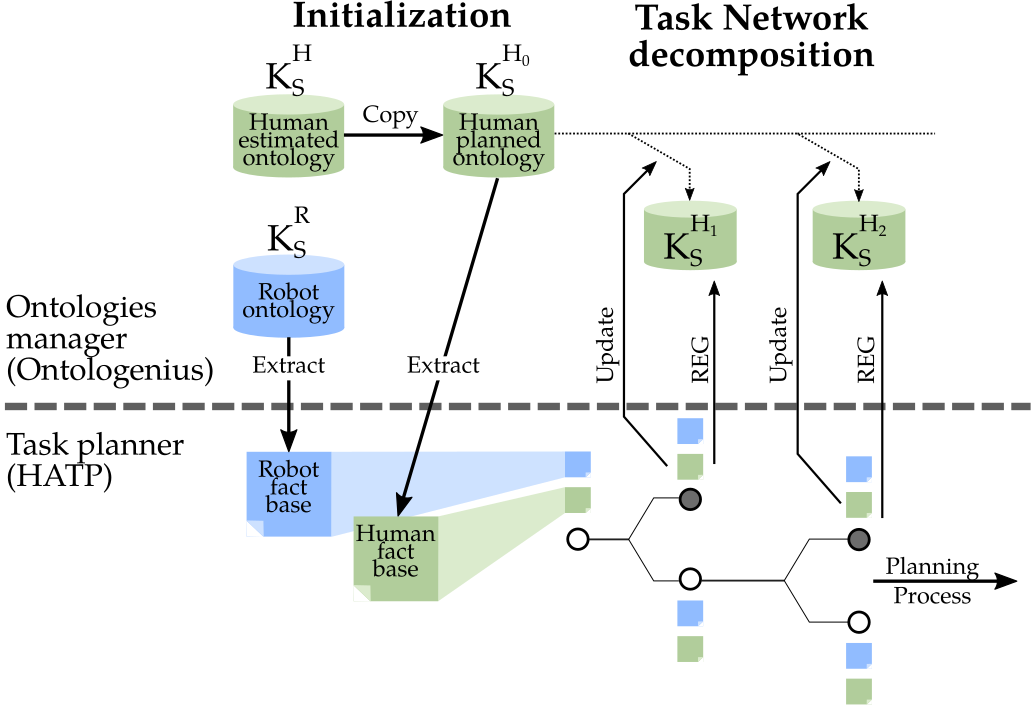
\includegraphics[scale=0.4]{figures/chapter5/integration.png}
\caption{\label{fig:chap5_integration} A representation of the planning process with the estimation of future human mental states to perform REG. The ontology representing estimated human knowledge is first copied to plan it without altering the original one. The human and robot planning symbolic facts are extracted from their respective ontologies. During the HTN decomposition, for each verbal communication action encounter, the planned human ontology is updated with the current explored state and the REG is executed on it. }
\end{figure}

In this section, we explain how a communication action is represented in the HTN and how the task planner can easily update the human planned ontology. We will even go further with an unimplemented update solution that could reduce the number of updates to be performed. 


\subsection{The representation of the communication action}

To focus ourselves on communication actions, we have thus designed simple planning problems where only the robot knows the goal of a joint task and issues command to its human partner one at a time when the human has to do an action. Communications related to entities of the scene are thus needed in each step of the plan because the human has no way to guess the actions he has to perform. Even if these problems present major limitations regarding the \textit{when} to communicate it allows us to simply present our approach. However, the method is still applicable on more general problems which need to estimate the \textit{what} of communications and ensure their pertinence in future states. Moreover, the presented method is compatible with others focused on the estimation of the \textit{when} to communicate~\cite{devin_2016_implemented}, \cite{unhelkar_2020_decision}.

In the HATP domain it is represented in the way that when an abstract or a primitive task is only feasible by a human and requires to designate a specific entity, a decomposition is added. In this decomposition, we specify that if the task is assigned to a human, a referring communication action must be done before by the robot to this human. This kind of decomposition is needed because we place ourselves in cases where the humans do not know the global objectives of the task, and thus, all the instructions must be given by the robot. With this approach, we consider that the human needs communication from the robot to act, and does not plan by themselves. In a more general case, the communication action from the robot would only appear if humans do not have the necessary information~\cite{devin_2016_implemented}. An example of plan is represented in Figure~\ref{fig:chap5_plan}.

\begin{figure}[!ht]
\centering
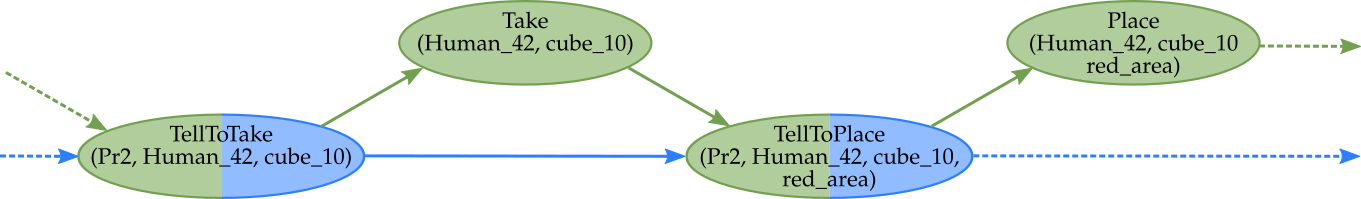
\includegraphics[width=\textwidth]{figures/chapter5/plan.png}
\caption{\label{fig:chap5_plan} An example of a plan generated by HATP where the robot instructs to take an object then place it in an area. Green actions are performed by the human while the bicolor actions involve both agents. }
\end{figure}

The communication action feasibility is then determined by both symbolic preconditions (e.g. the human and the robot are in the same room) and REG result (whether a solution is found or not). If the communication action is feasible, the cost of the communication action is then computed as the sum of a fixed cost depending on the type of communication and the REG solution cost. If multiple entities would have to be referred in a single communication, the cost would be the sum of each REG solution cost and the fixed cost.

\subsection{Maintaining the right knowledge base, at the right time}

We previously saw the need to keep an ontology updated with the estimated beliefs at the time of the communication to run the REG on it and the necessity to create the human planned ontology with a copy of the human estimated one to not create side effect on the rest of the architecture.

Since maintaining this external representation can be a heavy process, we first choose to only update it when a communication action has to be evaluated. However, having a single planned ontology, knowing the update to perform on it to reflect the current explored state can be an intractable problem. The planner can perform so backtracking during the exploration and the modifications to perform to represent the state of the currently evaluated communication would depend on the previous communication action explored. Because the previous communication could come from a side decomposition, the planner would have to either compare each relation between its representation and the ontology or keep a trace of all the modifications between two successive evaluations.

A first solution would be to create a copy of the planned ontology representing the initial state in order to have one ontology for each communication evaluation, all create from the initial state. Such a solution would reduce the planner complexity but as the ontology represent a superset of the planner facts base, it would be too time-consuming for the ontologies manager. For huge ontologies, analyzing the modification between two updates would be faster than an entire copy.

\begin{figure}[!ht]
\centering
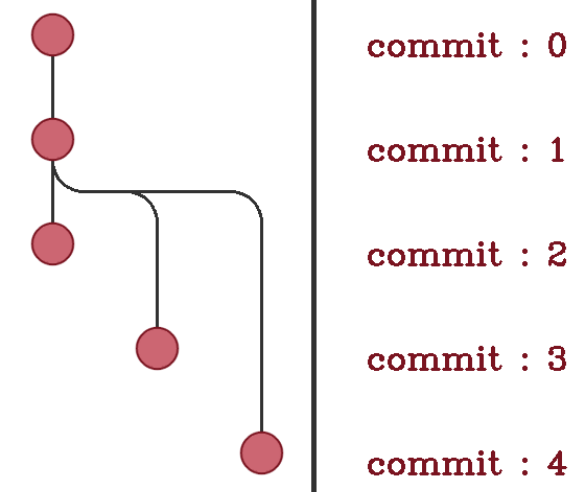
\includegraphics[scale=0.3]{figures/chapter5/versioning_simple.png}
\caption{\label{fig:chap5_versioning_simple} The commit-graph generated by Ontologenius for a plan with three communication action evaluated. Each evaluation generate a specific commit representing the state of the world at the moment of the communication. }
\end{figure}

To solve this problem we thus choose to use a versioning system on the ontology. This versioning system is the one proposed by the software Ontologenius presented in chapter \change{ref to chapter} \footnote{For the story of this thesis, this feature has initially been developed especially for this application after we had evaluated that a simple task would require few hours to be solved.}. We thus keep the first step that is to create the planned ontology with a copy then perform a commit on it to mark this initial state. From there, when a communication action is found, the planner goes back to the initial commit and update the ontology with the difference from the initial state. However, HATP is not adapted to keep such trace and it would require too many modifications in its internal structure. To passe over this problem, the planner performs a first commit to represent the initial state and extract the necessary knowledge from it. It then removes all the dynamic relations from the ontology a perform a second commit. It will represent a kind of pattern for each state involving a communication action. For each of them, the planner just has to go back to the commit representing this pattern and update all the dynamic relations with their values in the evaluated state. An example of a commit-graph related to this solution is represented in Figure~\ref{fig:chap5_versioning_simple}. Each commit thus represents a $\kbs^{H_i}$ on which a REG can be performed. The advantage here is that the knowledge backtracking is internally managed by Ontologenius and thus optimized.

\subsection{Reducing the number of updates}

A major limitation of the previous solution is the need to update all the dynamic relations even if few changes between communications. An unimplemented but feasible solution would be to update the ontology for each explored state during the planning process and create a commit for each of them. The advantage is that the backtracking has not to be managed by the task planner and only the modified relations have to be updated in the ontology. A commit-graph of such solution is represented in Figure~\ref{fig:chap5_versioning_advance}. Assuming this graph to represent the same task decomposition of the previous one, we see however that more commit have to be performed even if fewer modifications are performed between the two. For tasks with many communication actions, it could lead to a performance gain but for tasks with less communication, it would require more updates than needed as even decompositions without communication have to update the ontology.

\begin{figure}[!ht]
\centering
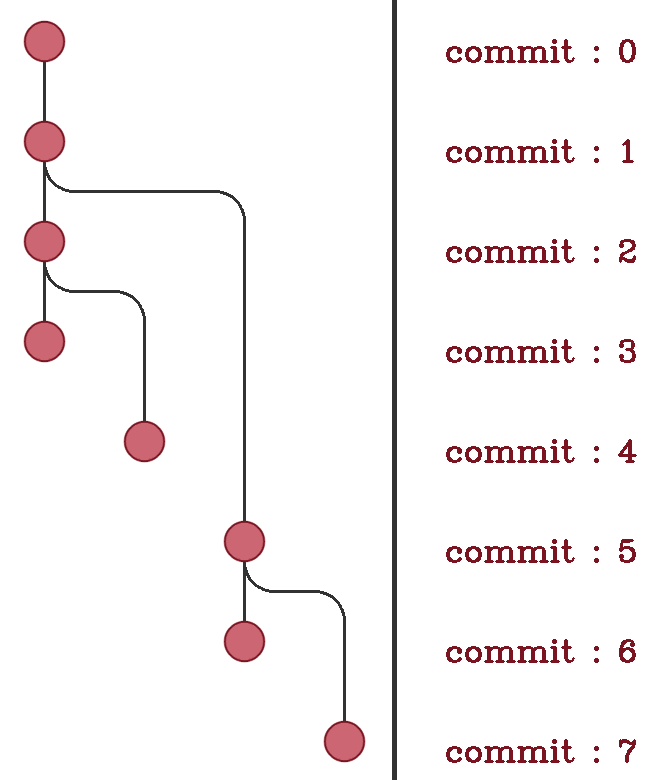
\includegraphics[scale=0.25]{figures/chapter5/versioning_advance.png}
\caption{\label{fig:chap5_versioning_advance} The commit-graph generated by Ontologenius for a plan with three communication action evaluated. Each exploraed state, with ou without communication action, generates a specific commit representing the state of the world at the moment of the action. }
\end{figure}

From the planner point of view, it would just have to assign UID to each state and created a commit using these UIDs. When backtracking, it would just have to checkout the ontology with the UID of the state to explore.


\section{Results}

In this section, we present three case studies. The two first ones are run in simulation only minimalist setups. They respectively show that the estimation of the communication content during the task planning 1) can prevent from execution dead-end and 2) can reduce the global communication complexity during the task. The third case study is run on a PR2 robot. It shows that our method makes it possible to compare different means of communication and to choose the most appropriate. The integration in the robotic architecture is presented in the next section.

All the three cases studies are based on a cube arrangement task in the same principle of the RFID tag arrangement presented in introduction. The human can only distinguish the cubes by their color and the digit written on them (one or two) if there is one. Three colored storage areas are cover the entier surface of the table. An object is thus always in one of the areas. The area in which the cube is an aditional information usable for the communication. The more complet RE is of the kind of: \textit{"the green cube with the number 2 which is in the black area"}. For the three cases, only the robot knows the goal configuration but can not manipulate them. It thus has to guide the human in the arrangement task. The robot can only point the cubes in the third case study. In the first two, he can only use verbal communication.

\subsection{Prevent execution dead-end}

In this first case study, we consider the introduction example recall in Figure~\ref{fig:chap5_case1} with the initial state (left) and final state (right). The cube C1 has to be moved from the red area to the black area. The cube C2 has to be moved from the black area to the white area. The cube C3 does not have to be moved.

\begin{figure}[!ht]
\centering
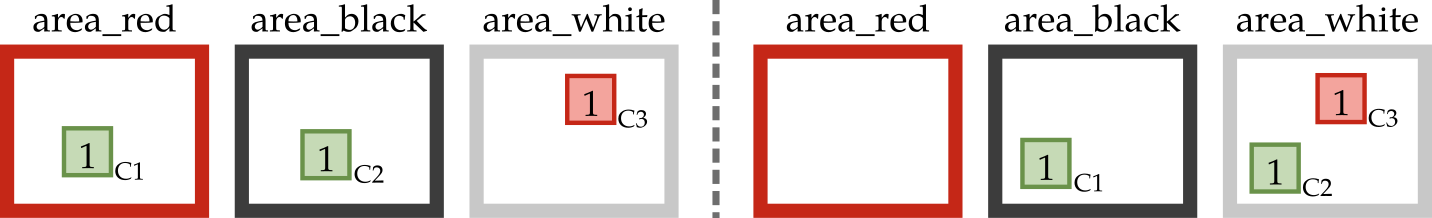
\includegraphics[width=\textwidth]{figures/chapter5/results_case1.png}
\caption{\label{fig:chap5_case1} The initial state (left) and final state (right) of a task where the robot has to explain to the human partner how to move the cubes to complete the task. In this situation, explaining C2 first then C1 avoids a dead-end. }
\end{figure}

Taking into account the cost and the feasibility of the communication, we found with our method the plan of listing~\ref{lst:chap5_case1}. Cube C2 is moved first then the cube C1. Doing the inverse order, after moving C1, the two cubes would be in the black area at the same time. Such a situation would cause a dead-end during the execution of the plan or at least require complex communication. Actions prefixed with HR are performed simultaneously by the robot and the human while the actions prefixed by H are only performed by the human. As a comment of each action are the relations to communicate.

\begin{lstlisting}[frame=single, basicstyle=\scriptsize\ttfamily, label={lst:chap5_case1}, caption={The obtained plan for the first case study where cube C1 must be moved from the red to the black area and cube C2 moved from the black to the white area. The lines beginning with H represent the actions of the human and the lines beginning with HR represent actions involving the human and the robot (communication actions). In green are the REG results for each communication action.}, captionpos=b, style=HatpPlan]
HR - TellHumanToTake(C2) // (C2, isA, Cube), (C2, isIn, area_black), 
                         // (area_black, isA, Area), 
                         // (area_black, hasColor, black)
H  - Take(C2)
HR - TellHumanToPlace(C2, area_white) // (area_white, isA, Area),
                                      // (area_white, hasColor, white)
H  - Place(C2, area_white)
HR - TellHumanToTake(C1) // (C1, isA, Cube), (C1, isIn, area_red), 
                         // (area_red, isA, Area), (area_red, hasColor, red)
H  - Take(C1)
HR - TellHumanToPlace(C1, area_black)  // (area_black, isA, Area),
                                       // (area_black, hasColor, black)
H  - Place(C1, area_black)
\end{lstlisting}

Considering once again the same initial state but with the goal to invert the positions of the two cubes, if the communication cost and feasibility are not taken into account during planning, both actions directly leading to the goal state (\textit{i.e.} cube C1 moved to the black area or cube C2 to the red area) will lead to a dead-end at plan execution. To solve this situation, the task planner chooses to add a supplementary action. It consists of putting the cube C1 in the white area that then leads to a problem similar to the previous one. This additional action avoids a dead-end by making communication about cube C2 feasible. Another solution could have been to move C2 in the white area first, leading once again to a situation comparable to the previous one.


\subsection{Reduce the overall communication complexity}


\begin{figure}[!ht]
\centering
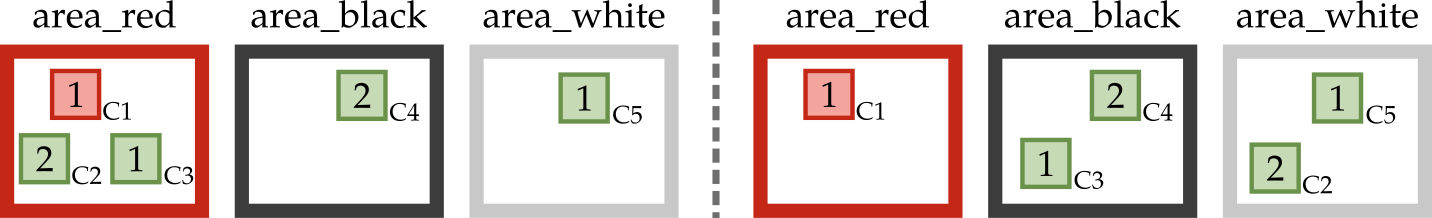
\includegraphics[width=\textwidth]{figures/chapter5/results_case2.png}
\caption{\label{fig:chap5_case2} The initial state (left) and final state (right) of a task where the robot has to explain to the human partner how to move the cubes to complete the task. In this situation, explaining C2 first then C3 is easier than the inverse. }
\end{figure}

In this second case study, we show how the estimation of communication can be used to reduce the complexity of global communication. We consider the initial state and the goal state represented in Figure~\ref{fig:chap5_case2}. Only cubes C2 and C3 should be moved. Our method finds the solution consisting of moving cube C2 first, then cube C3. With this order, cube C2 is referred by three relations: its type (\textit{i.e.} cube), the number on it and the colored area in which it is located. After that, the cube C3 can also be referred to only by three relations being its type, its color and the colored area in which it is located. Considering the reverse order, this would have generated a more complex RE first for cube C3 with four relations: its type, its color, the number on it and the colored area in which it is located.
The solution chosen by our method communicates a sum of six relations rather than seven with the reverse order.

\subsection{Compare with other communication means}

In this last case study, we show how the estimation of verbal designation communication cost can be used to compare it with other communication means, here pointing. Now, we consider twelve cubes. The initial state and the goal state are represented in Figure~\ref{fig:chap5_case3}. Such a number of similar objects leads to long explanations to refer to certain cubes. Therefore, we aim the task planner to choose another means of communication to refer to cubes too difficult to explain verbally. The pointing action has a constant cost which is higher than simple verbal communication but lower than a complex one (with three or more relations to verbalize). To exemplify the comparison with other communication means, the arrangement order is predefined in this setup.

\begin{figure}[!ht]
\centering
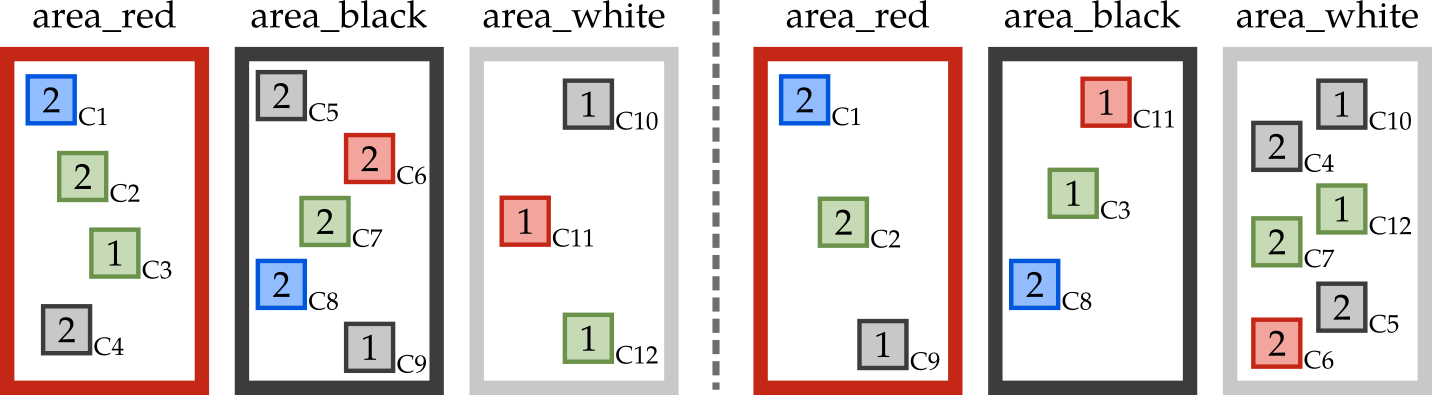
\includegraphics[width=\textwidth]{figures/chapter5/results_case3.png}
\caption{\label{fig:chap5_case3} The initial state (left) and final state (right) of a task where the robot has to explain to the human partner how to move the cubes to complete the task. In this situation, some cubes are too complex to explain. Pointing them could help in some cases. }
\end{figure}
 
The cubes C5 and C7 are chosen to be pointed instead of verbalized. Indeed, in the world states where these cubes need to be moved, verbal referring is considered to be too costly, thus a pointing motion is preferred. For example, the cube C5 in the initial situation needs a long and complex explanation that is: \textit{"take the black cube with the number two which is in the black area"}. Even in the case the pointing action takes more execution time, it could require less cognitive load for the human partner and so make the human action faster.

Here, we see another benefit of our approach, it allows the planner to balance between the use of verbal communication actions, which can become complex in some states (hard to predict without a task planner), and other communication modalities. Here, balancing was done with other means of communication, but it could also be done with other actions such as a pick and place by the robot. In the task presented here, this has no advantage, because a pick and place by the robot would be slower than an explanation or a pointing and is more likely to fail.

\section{Integration in a robotic system}

The third case study has been implemented on a pr2 robotic platform. We extend the previously used architecture and integrate two new components as illustrated in Figure~\ref{fig:chap5_archi}. The execution of the third case can be found in the video available at \url{https://youtu.be/3YnGh_t-UpY}.

\begin{figure}[!ht]
\centering
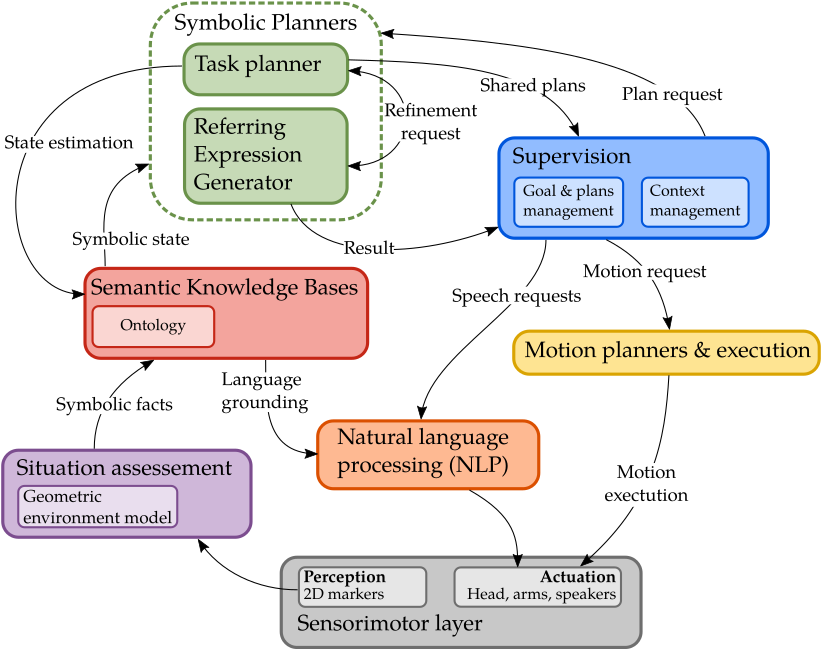
\includegraphics[scale=0.6]{figures/chapter5/architecture.png}
\caption{\label{fig:chap5_archi} The architecture used to validate the method. The knowledge bases are continuously kept up to date through the situation assessment. The task planner can query the REG to estimate the feasibility and cost of future communications. }
\end{figure}

The Symbolic task planner is HATP. It is requested by the supervision component which is able to manage the execution of the generated shared plan. The task planner can recover the initial state from the semantic knowledge base and update an ontology instance to represent the human future estimated knowledge base. In addition, it can request the generation of referring expression on a human planned ontology.

The second newly integrated component is a motion planner and execution component. For now, it only provides to the supervision a pointing service and automatically chooses the arm to point with. However, it does not consider the obstacles.

The geometrical situation assessment component has been changed from Robosherlock to a custom version of Toaster\footnote{https://github.com/sarthou/toaster}. It is the successor of the software SHARY~\cite{milliez_2014_framework}. It can take as input several perception modalities and merge them in a coherent geometric representation. For our implementation, we simply use AR-tags which give precise enough position and allow us to identify objects with UIDs. The table and other static elements of the environment are not perceived and provided as static elements. The three storage areas are neither perceived and described as 3D virtual areas. Thanks to these areas, Toaster is able to compute the fact \textit{isIn} for each of the cubes. From there, Toaster has been linked to Ontologenius to update the ontologies continuously. A representation of Toaster geometric environment is represented in Figure~\ref{fig:chap5_toaster}.

\begin{figure}[!ht]
\centering
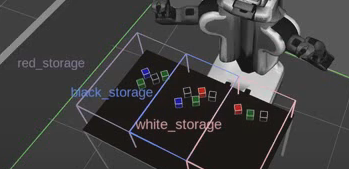
\includegraphics[scale=0.70]{figures/chapter5/toaster.png}
\caption{\label{fig:chap5_toaster} A visual representation in Rviz of the geometric state of the managed by Toaster. While the cubes are perceived with tags, the other elements are static.
 }
\end{figure}

A major limitation of the current situation assessment component is that it can not perform perspective-taking. This means that even if it can represent the human as a particular entity, it can not estimate the state of the world from the human point of view\footnote{We can compute if an object is in the field of view of the human but not working with a graphical engine, it can not take into account the occlusions.}. It is not a problem for our application since all the elements are visible for both agents and the entire interaction is performed around the table. Toaster thus updates the robot and human ontologies with the same facts.

\ifdefined\included
\else
\setcounter{chapter}{6} %% Numéro du chapitre précédent ;)
\dominitoc
\faketableofcontents
\fi

\chapter{Extending the REG with knowledge about past activities}
\chaptermark{REG with knowledge about past activities}
\minitoc
\label{chap:6}

Taking advantage of the link previously made between the ontology, the human-aware symbolic task planner, and the \acrshort{reg} solver, we propose in this chapter a new way to generate \acrlong{re} based on agents past shared experience. Among this chapter, we first propose a representation of \acrshort{htn} as well as execution trace using an ontology. Then we extend the \acrshort{ucs}-based \acrshort{reg} algorithm to consider this new knowledge as a piece of information, usable to generate \acrlong{re}.

The contribution presented in this chapter is excerpted from our work, published in the proceedings of the IROS 2021 conference~\cite{sarthou_2021_extending}. In this manuscript, the contribution is more detailed and discussed. In the continuity of the two previous, the presented work has been achieved in collaboration with Guilhem Buisan. He brought his expertise on HTNs to allow the best possible representation in an ontology.

\section{Introduction}

When two or more agents perform a collaborative task, although they may have a different perception of their shared environment, they can estimate the information they share and can thus use it to communicate about entities they estimate to be known by the others. This assumption is the one commonly used to develop and evaluate \acrfull{reg} methods through the use of caption of the environment\cite{duboue_2015_evaluating}. These captions are images always taken from the hearer point of view. The image, or the related knowledge representation, is provided to the algorithm which has to generate a referring expression. This assumption has also been used when the \acrshort{reg} has been applied to \acrfull{hri} and can be compared to a robot spawning in an environment and having to designate an object. However, this designation occurs during a joint activity between a robot and a human partner meaning that the designated objects may have been used, moved, or already talking about. All of this information about the performed task can be seen as additional knowledge shared by the involved agents. We can thus refer to the entities through these past actions in addition to their attributes and relations with each other.

\begin{figure}[ht!]
\centering
\includegraphics[width=\textwidth]{figures/chapter6/intro/intro.png}
\caption{\label{fig:chap6_intro} Referring to knife \textit{k2} in the current situation (\textit{t3}) is impossible if the robot is performing an action that does not allow it to see what is in front of the human. Considering previous steps of the human's task, the robot can refer to the knife through the action to cut a tomato (\textit{t2}) or to cut a cucumber (\textit{t1}).}
\end{figure}

Consider the caption of the interaction represented in Figure~\ref{fig:chap6_intro} at the current instant \textit{t3}. The robot, in the back of the kitchen, has to ask the human for the knife \textit{k2}. Since the robot is performing another action of the joint task, it cannot see what is in front of the human. Consequently, it cannot know and thus use any spatial relations about \textit{k2}\footnote{We could also consider an object known by the robot but for which it does not have any information regarding its new location and searching for it. It would have to refer to it, to ask for the human help, without the possibility to use spatial relations.}. Therefore, the robot can only use \textit{k2} attributes (i.e. only its color) to generate an expression referring to it. Still considering only the current instant \textit{t3}, two other blue knives hold in the kitchen being \textit{k1} and \textit{k3}. The knife \textit{k1} is fixed to the wall in front of the robot meaning that it is already accessible to it and not to the human. This knife can thus be considered as being out of context and not leading to any ambiguity with \textit{k2}. The other blue knife \textit{k3} remains ambiguous since it has no perceptible attribute that differs from the one the robot has to refer to.

Until now, we have only considered the current situation \textit{t3} and not the human-robot shared experience about the task they perform. At the previous instant \textit{t2} the human was cutting a tomato with the knife \textit{k2}. It was manifest to the human that the robot was observing the scene while he acted. This new information about the performed action could thus be used by the robot to generate a reference to the wanted knife in the current situation. A possible \acrshort{re} would be ``\textit{the knife with which you cut the tomato}''. 

Consider now the action a step before cutting the tomato at instant \textit{t1}. The human was cutting a cucumber with this same knife. The combination of these two past actions can be seen as the task of preparing vegetables. The robot can thus also use this knowledge to refer to the knife. A possible \acrshort{re} considering the totality of the interaction would be ``\textit{the knife with which you prepared the vegetables}''. The exploitation of shared knowledge about past activities in addition to the usual attributes and properties could lead to the generation of richer \acrshort{re} that could be easier to understand by the human partner. Besides, it allows to generate REs in contexts where the previous method was not effective.

This chapter is an extension of our previous work~\cite{buisan_2020_efficient} presented in Chapter~\ref{chap:4}. It has been integrated within a cost-based Hierarchical agent-Base Task Planner to estimate the feasibility and cost of REs during the planning process~\cite{buisan_2020_human}, presented in Chapter~\ref{chap:5}. In this chapter we will thus aim to create the inverse link, making the \acrshort{reg} able to use execution traces resulting from the execution of hierarchical plans generated by \acrshort{hatp}. Like the previous chapters, we only focus on the content determination of the \acrshort{reg} problem but continue to consider the need to have names in natural language to enable linguistic realization.

The main contribution of this chapter is an extension of the ontology-based \acrshort{reg} algorithm by \textbf{considering past agents' activities}. A side contribution of this chapter is a proposal of a formalism to \textbf{represent Hierarchical Execution Traces} (executed \acrshort{htn}-based plans) in an ontology. Our previous contribution considered cost functions based on the properties of the used relations to represent the cognitive load required for a human to interpret the \acrshort{re}. In this extension, we propose to add customizable cost functions based on time, to represent the cognitive load required for a human to remember referred activities.

First, we review the literature concerning \acrshort{htn} representation in ontologies and discuss \acrshort{reg}-related works that not only consider caption of situations. Then, we describe the used knowledge bases and the usual structure of \acrshort{htn} and shared \acrfull{het}. We then give an overview of how the knowledge bases should be updated and we describe the content of these updates in terms of how a shared \acrfull{het} is represented in an ontology. The extension of the algorithm is then detailed before ending with an efficiency comparison regarding the original version (see Chapter~\ref{chap:4}) and a discussion around five illustrative cases to show the solutions found by our algorithm depending on the agent's knowledge about past activities.

\section{Related work}

In the previous chapter about \acrlong{reg} we already gave a good overview of the literature of the field. In this chapter, we thus briefly discuss few works trying to consider an interaction. We then move on to a wider part about the representation of \acrshort{htn} and execution traces in ontology to see the kind of information our algorithm could use to generate a new kind of referring expression.

\subsection{Interaction based Referring expression}

In all the previously presented works, the \acrshort{reg} is only performed on the current environment state. Williams in~\cite{williams_2020_toward} is the first to add a temporal aspect by considering a sequence of \acrshort{reg}. Like others before, he starts from the idea that to designate an entity it is preferable to use properties known by the hearer and that he/she will easily identify. Where other works, our included, represent that with cost on properties that we assume to be representative for the hearer, Williams tries to take advantage of an entire interaction. During such interaction, two partners will generate \acrshort{re}. The presented algorithm thus try to re-use properties used in previous descriptions made by the partner. In addition, he has implemented a forgetting model based on decay or interfering to avoid the use of properties used too long ago. This method has been tested on a ``Guess Who''-style game. This kind of game has the advantage that the used properties hold between the \acrshort{reg} and thus can be re-used. However, this assumption can no longer be maintained in a real dynamic interaction where objects are manipulated and their properties modified all along the interaction.

Early in the field, Oberlander and Dale already showed that generating references to eventualities (\textit{i.e.} to past activities or past events) can be done in the same way as generating references to physical entities~\cite{oberlander_1991_generating}. However, they never generate references to entities through the use of past actions. To close this short tour, Wiriyathammabhum et al. in~\cite{wiriyathammabhum_2019_referring} use \acrshort{re} involving past actions to identify a referred entity in videos but does not generate them.

%The determination of the properties' costs will not be discussed here but we can mention \cite{belke_tracking_2002} and \cite{koolen_learning_2012} which use learning techniques to estimate the users' preferences.

\subsection{HTN-based tasks representation in ontology}

In robotic and even more in \acrshort{hri}, storing semantic information about past activities is needed to generate training data~\cite{diab_2020_knowing} and learn from experience~\cite{petit_2016_reasoning}, or to speak about what happened~\cite{mealier_2017_narrative}. Some approaches represent the past actions using only structured sets of SQL tables~\cite{mealier_2017_narrative}, but such a representation lacks semantic information both on the involved entities (e.g. a robotic agent is a specific type of agent) and on the actions (e.g. a cut action is part of a salad preparation task). Since ontologies are fully suitable to represent semantic information about entities and their relations, they have been used to represent task planning knowledge. In~\cite{sun_2019_rtpo}, a Robot Task Planning Ontology (RTPO) is proposed but the model does not consider the rich semantics involved by the hierarchical nature and intricacies of human-robot joint activities. For example, they represent the fact that the action ``ChargeAction'' is a ``ChargeTask'' while a more correct semantic would be that the ``ChargeTask'' is composed of a ``ChargeAction''. However, their representation does not allow such a correct semantic representation.

To represent episodes, the EASE-CRC has put forward the concept of narratively-enabled episodic memories(NEEMs)~\cite{diab_2020_knowing}. Build from annotated perception events and sensor data, they provide comprehensive logs of tasks performed by the robot. The annotations are based on the terminology provided by the Socio-physical Model of Activities(SOMA)~\cite{bessler_2020_foundations}. It proposes a high-level description of what is an event or an object in addition to the notion of plan. However, a plan is just a succession of actions and this terminology thus does not support the use of \acrshort{het} for the moment. A design pattern for the representation of such NEEMs in ontology has been proposed in~\cite{bernd_2020_modelling}. However, this pattern is too cumbersome for ontology developers and not practical to use in side-fields for which the safety of data input is not mandatory for the moment.

\acrshort{htn} is a very popular way for representing, planning, and controlling autonomous agents' activities \cite{ghallab_2004_automated, ingrand_2017_deliberation}. It is a tree representing how to decompose abstract tasks into primitive tasks directly applicable by an agent \cite{erol_1994_htn}. They are widely used for robotic planning as they allow to efficiently find complex plans by choosing between different task decompositions depending on the world state. 
Unlike more classical state-space search-based planning algorithms like STRIPS~\cite{fikes_1971_strips}, \acrshort{htn} planning does not explore applicable actions until a goal is reached, but rather tries to fully decompose an abstract task into applicable primitive tasks. Moreover, \acrshort{htn} planning is often quicker as domains (\acrshort{htn} representations) are provided with expert knowledge through the hierarchical structure and task decomposition alternatives. 
In \acrshort{hri} scenarios, their usefulness is even more apparent. In \cite{lallement_2014_hatp}, an \acrshort{htn} is used to generate human-robot joint plans. Furthermore, the hierarchical structure can be used to negotiate or communicate about high-level plans when details about realisation do not matter~\cite{milliez_2016_using}. As an example, for a robot equipped with a charge plug and solar panels, an \acrshort{htn} may represent the abstract task of ``ChargeTask'' as being decomposed into either ``GoToChargeStation'' primitive (or abstract) task or ``GoOutside'' task. An \acrshort{htn} planner would then explore these alternatives and generate the most appropriate plan depending on the current world state, here, the current weather.

To the best of our knowledge, few works exist on the representation of an \acrshort{htn} and their \acrfull{het} in ontologies. Umbrico et al. in~\cite{umbrico_2020_ontology} describe the notion of complex tasks composed of simple tasks but do not go further in the representation. In \cite{freitas_2014_using} only the planning domain is represented. The major issue is that the ontology classes are used to describe the general \acrshort{htn} concepts (i.e. action, method) while the field concepts (e.g. the cut task in our example) are described using the ontology individuals. Hence, this representation does not make it possible to represent instantiations of abstract or primitive tasks. This distinction between the domain as a high-level knowledge and thus represented in the ontology classes and properties on one side, and the \acrshort{het} representation as an instantiation of this domain on the other side is important to us. It allows to both represent how a given task could be done and how it has been done during execution. Our work is closer to BOWL~\cite{ko_2011_business}, an \acrshort{htn} ontology for business process representation. Even if they have defined some specific relations for the Business-to-Business field, the general tasks, decomposition, and tasks links representation are interesting. However, BOWL only represents the \acrshort{htn} and not \acrshort{het}s, but does not preclude it.

\section{Structuring and gathering the knowledge}

In this section, we first present the main knowledge structures necessary to perform the extended \acrshort{reg} through shared knowledge about past Human-Robot collaborative activity. We continue with an overview of the robotic architecture allowing us to acquire this knowledge, to understand the knowledge to be acquired offline and those to be acquired during the interaction. We end this section with the proposed terminology to represent \acrshort{htn} and \acrshort{het}s in the ontology.

\subsection{The three used knowledge representation}

Three knowledge representations are used and can be grouped into two categories: the dynamic and static ones. The dynamic part is updated all along the course of the interaction. It is defined as $\kb = \langle \kbs, \kbe \rangle$ with $\kbs$ the semantic part already presented (see Section~\ref{sec:kb_formalism}) and $\kbe$ the episodic part. The static knowledge base represents the planning domain as a \acrfull{htn}.

\subsubsection{The Hierarchical Task Network}

In the previous chapter, we saw that an \acrshort{htn} is a way of representing a task to be planned, meaning to be fully refined and instantiated. In the present section, we go deeper into the \acrshort{htn} and give a more formal definition based on~\cite{erol_1994_htn}.

An \acrshort{htn}, noted $\HTN$, is defined as a set of tasks $\tasknetwork$. A task $\task$ is represented by a task name associated with a list of typed arguments. Taking the \acrshort{htn} illustrated in Figure~\ref{fig:chap6_domain}, the task \textit{cut} has the arguments \textit{A, V, K}, which are respectively an agent, a vegetable, and a knife. The general term task can be refined into \textbf{primitive task} ($\task \in \primtaskset$ with $\primtaskset$ the set of primitive tasks) or \textbf{abstract task} ($\task \in \abstaskset$ with $\abstaskset$ the set of abstract tasks). A task is said to be primitive if it does not need refinement meaning that it can directly be executed by the robot or by a higher-level component\footnote{Primitive tasks usually have preconditions and effects. We do not describe them in this thesis as they are not used.}. An abstract task needs further decomposition and can not be executed by the robot as it is. In Figure~\ref{fig:chap6_domain}, \textit{PrepareSalad()} is an abstract task while \textit{cut(A,V,K)} is a primitive task.

Then, we define the set of decompositions $\decomposet$. A decomposition is a pair $(\abstracttask, \tasknetwork) \in \decomposet$ where $\abstracttask \in \abstaskset$ is an abstract task and $\tasknetwork$ a set of tasks describing one way of decomposing $\abstracttask$. In Figure~\ref{fig:chap6_domain}, the abstract task \textit{PrepareVegetable(A,K,V)} has two decompositions \textit{d8} and \textit{d9}. Moreover, among the tasks set of a decomposition (i.e. the tasks used by the decomposition), can be enrich with a precedence order in which the tasks have to be performed. For example, in Figure~\ref{fig:chap6_domain}, the tasks \textit{peel(A, V, K)} and \textit{peel(A, V, K)} are totally ordered under the decomposition \textit{d8}. 

\begin{figure}[ht!]
\centering
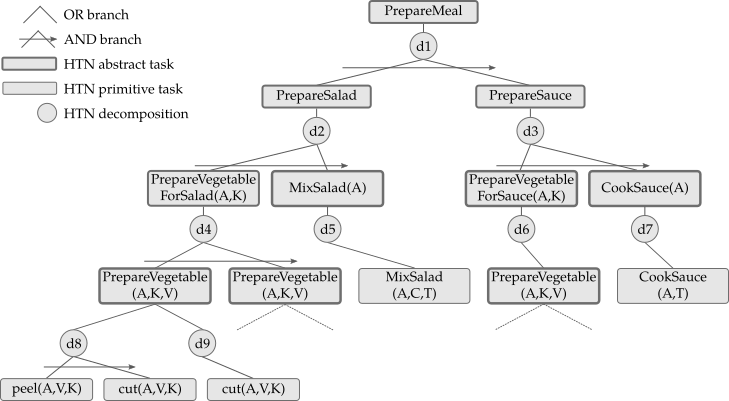
\includegraphics[width=\textwidth]{figures/chapter6/domain.png}
\caption{\label{fig:chap6_domain} The  domain of the high-level task \textit{PrepareMeal}. It is used by the planner (\acrshort{hatp}) to elaborate a Human-Robot shared plan through a context-based decomposition and parameter instantiation process (which vegetable V, which knife K, ...) including the selection of the agent A (Tony the human, or PR2 the robot) to which the abstract tasks and/or the primitive tasks will be allocated.}
\end{figure}

Given an initial world state and an initial task to decompose, a planner such as \acrshort{hatp} elaborates a plan through successive decompositions from the initial task and respecting the constraints issued by the initial world state. A resulting plan is a sequence of primitive tasks. The planner thus tries to recursively select a decomposition for each abstract task encountered until it reaches primitive tasks. Besides, the planner has to ground every argument of the tasks into entities of $\Abox$ (the ABox of the knowledge base $\kbs$) while respecting constraints regarding their types.

\subsubsection{The semantic and episodic knowledge bases}

The semantic knowledge base $\kbs$ is an ontology as described earlier. The episodic knowledge base $\kbe$ is a timeline also called datebase~\cite{allen_1983_maintaining}. It maintains temporal reference for every fact that varies in time. Representing only the changes, we can assume that a fact holds between two changes.

We defined it as a pair $\kbe = ( \{ \langle \relation, \tau \rangle \}, \{ \langle \taction, \tinterval \rangle \} )$. The first element is a set of time-stamped relations like a classical datebase. The second element aims at representing the performed tasks. It is a set of pairs with $\taction$ an instance of a task and $\tinterval$ a temporal interval composed of two numerical values. The tasks defined in $\kbe$ are also represented as entities of $\kbs$ ($\taction \in \indivset$). Since they are semantically represented in $\kbs$ we can, inter alia, retrieve their types or arguments.

\begin{figure}[h!]
\centering
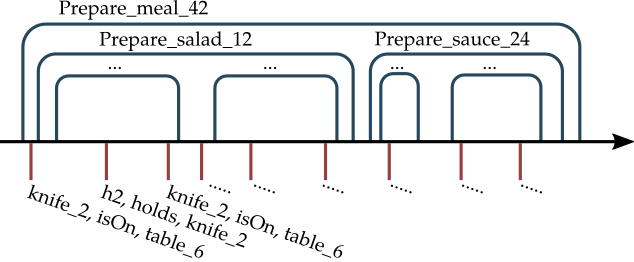
\includegraphics[scale=0.55]{figures/chapter6/ke.png}
\caption{\label{fig:chap6_ke} An example of timeline: On the upper part of the arrow are the tasks performed with their intervals. On the lower part are the relation changes.}
\end{figure}

Since we address \acrshort{hri} applications, in the same way, it has been done previously with the semantic knowledge base, we consider that the robot maintains a semantic and episodic knowledge base per human it is interacting with ($\kbs^{Hi}$ and $\kbe^{Hi}$ ) in addition to its own ($\kbs^{R}$ and $\kbe^{R}$). While the robot's own knowledge base is its personal truth, the agents' knowledge bases represent its estimation of the knowledge of its human partners.

\subsection{The knowledge gathering scheme}

We give now an overview of how the three knowledge bases are interconnected and how the semantic and episodic ones are updated. A minimal robotic architecture allowing the gathering of the necessary information is represented in Figure~\ref{fig:chap6_architecture}.

\newpage

\begin{figure}[ht!]
\centering
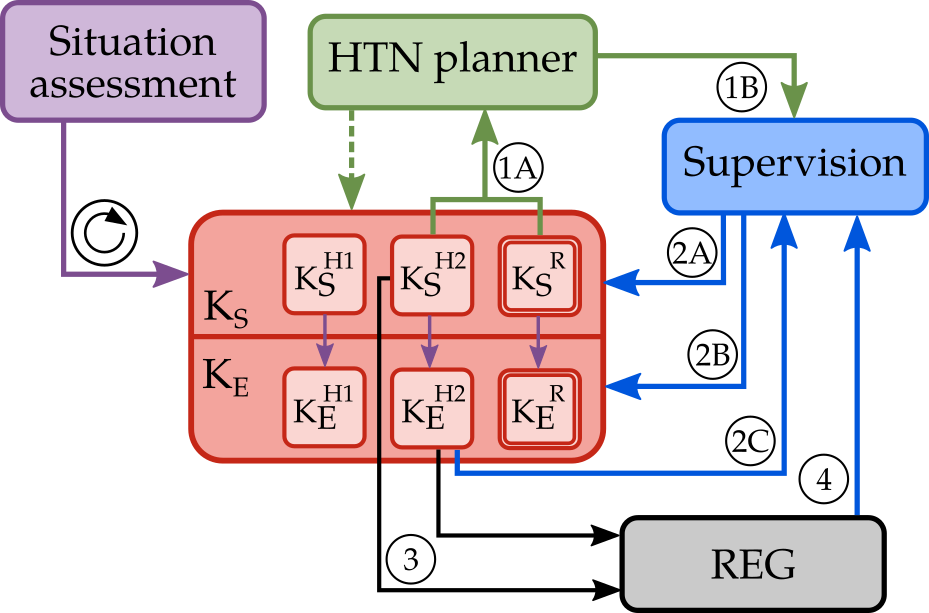
\includegraphics[scale=0.37]{figures/chapter6/architecture.png}
\caption{\label{fig:chap6_architecture} A ``minimal'' robotic architecture (based on the architecture presented in Figure~\ref{fig:chap5_archi}) allowing to acquire and store the knowledge necessary to perform a \acrshort{reg} using the past human-robot activities. The dotted arrow represents an offline acquisition, meaning knowledge acquired before powering on the robot. The other arrows are online interactions between the components. The numbering represents the execution order during the execution of a task.
The robot knowledge bases ($\kbs^{R}$ and $\kbe^{R}$) and the estimated mental states of its human partners ($\kbs^{Hi}$ and $\kbe^{Hi}$) are updated permanently by the Situation Assessment component which tracks changes in the environment and by the robot supervisor which controls robot planning and execution activities and monitors humans actions.}
\end{figure}

First of all, the task decomposition description stored as an \acrshort{htn} is parsed offline. We aim at extracting from it a semantic description of the tasks composing it (abstracts and primitives), their parameters, and their hierarchical links through the decompositions. All these descriptions are then stored into the ontology as classes and properties (dotted arrow on Figure~\ref{fig:chap6_architecture}) in order to ground future traces of execution.

Once the ontology is initialized with a common ground, containing the description of the planning domain, we can start the interaction. During the interaction, the situation assessment updates the semantic \acrshort{kb} of each agent with relations to the entities of the environment. Upon receipt of these facts, the semantic knowledge base temporally stamps them and stores them in the episodic knowledge base. It can also infer new facts thanks to the reasoning mechanisms. These inferred facts are also temporally stamped and stored in the episodic knowledge base\footnote{For now, only the performed tasks will be used to generate the REs but we still wanted to have a more general scheme to understand the context in which we want to use it.}.

On request of the supervision module, the \acrshort{htn} planner takes its initial world state from the ontologies of the involved agents (1A) and generates a shared plan (1B). During the execution of the shared plan, the supervision describes the performed tasks semantically (detailed in the following subsection) (2A) and stamps them in the timeline (2B) with their respective start and end times. While it knows the tasks performed by the robot, it needs to gather data from the episodic knowledge base of the human partner (2C), to monitor their tasks. Descriptions of the tasks are not stored in the episodic knowledge bases as not having any temporal mean. It would be nonsense to say that a task has a given parameter at a given time. We first describe it as having parameters on one side (2A) and then we describe when the task has been performed on the other side (2B). 

Upon a \acrshort{reg} request from the supervision, the \acrshort{reg} component explores the listener's both semantic and episodic knowledge bases (3) and returns the generated \acrshort{re} (4).

When the supervision component inserts the executed tasks in the semantic knowledge base, it thus creates a \acrfull{het}. The execution trace can differ from the initial plan since it can be the result of plan repair or re-planning steps within the same global task achievement. The \acrshort{het} thus contains the actions which have been performed and their link to the higher level of abstraction. No forgetting mechanism is considered since we focus on ``short'' interactions (few hours) but adding one would avoid the knowledge bases to grow indefinitely and could also be used to represent the human forgetting mechanism. This could be for future work.

\subsection{Building the ontology}

The aim of the following representation is not for planning per se (since this is done by the human-aware task planner) but rather to allow to store and manipulate a description of the execution of the human-robot shared plans together with their hierarchical structure and the information provided by the situation assessment component.
What is provided is the hierarchical task decomposition together with a semantic description of the entities used as tasks parameters, their properties, and relations to other entities in the environment. Moreover, the descriptions presented below are automatically generated from a \acrshort{hatp} domain and plan description~\cite{lallement_2014_hatp}.

\subsubsection{HTN in ontology}

An \acrshort{htn} represents the general knowledge about how to decompose high-level abstract tasks into executable primitive tasks. Since it is a piece of general knowledge, we represent it in the TBox and the RBox of the ontology. It allows instantiating the executed plan as individuals of the ontology. As a reminder, the list of the symbols used to describe an ontology, and thus used in this section, are summarized in Table~\ref{tab:onto_symboles}.

\begin{figure}[h!]
\centering
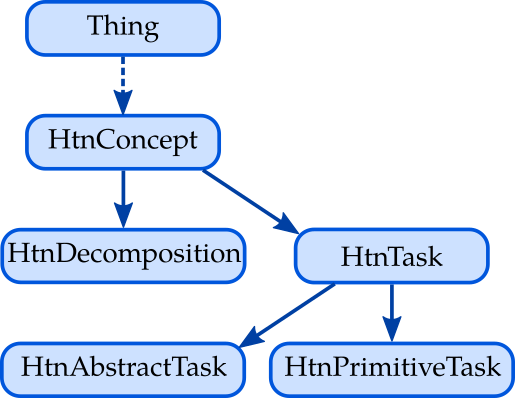
\includegraphics[scale=0.4]{figures/chapter6/tbox_base.png}
\caption{\label{fig:chap6_tbox_base} The upper classes used to decribe an \acrshort{htn}.}
\end{figure}

We first define the classes and properties common to any \acrshort{htn} representation. As shown in Figure~\ref{fig:chap6_tbox_base}, the upper class in the TBox to describe an \acrshort{htn} is \textbf{HtnConcept} from which the \textbf{HtnDecomposition} and \textbf{HtnTask} classes inherit. The HtnTask class is then refined into \textbf{HtnAbstractTask} and \textbf{HtnPrimitiveTask}.
The RBox is composed of the properties \textbf{hasDecomposition}, \textbf{hasSubtask}, \textbf{hasParameter}, and their inverse (e.g. $(hasParameter, isParameterOf) \in \invset$). The property $hasDecomposition$ links an abstract task to its decompositions. The property $hasSubtask$ links a decomposition to the tasks (primitive or abstract) composing it. The property $hasParameter$ links a task to any other entity.

To represent an \acrshort{htn} $\HTN$ we thus create in the ontology a new class $\class$ for each :
\begin{enumerate}
	\item primitive task $\task$ such as 
$\task \in \primtaskset \Leftrightarrow \class \in \classset \wedge (\class,\ HtnPrimitiveTask) \in H$.
	\item abstract task $\abstracttask$ such as $\abstracttask \in \abstaskset \Leftrightarrow \class \in \classset \wedge (\class,\ HtnAbstractTask) \in H$.
	\item decomposition $\decompo$ such as $\decompo \in \decomposet \Leftrightarrow \class \in \classset \wedge (\class,\ HtnDecomposition) \in H$.
\end{enumerate}

For each decomposition $\decompo$ we describe the following relations using annotation properties:
\begin{enumerate}
	\item A decomposition comes from an abstract task such as $\abstracttask \in \tasknetwork \Leftrightarrow (\abstracttask,\ hasDecomposition,\ \decompo) \in \annotationset$
	\item A decompositions has sub-tasks such as $\decompo \in \decomposet \Leftrightarrow (\decompo,\ hasSubtask,\ \task) \in \annotationset$.
\end{enumerate}

To put it into practice, let us consider the abstract task \textit{PrepareVegetable} of the domain illustrated in Figure~\ref{fig:chap6_domain}. The generated OWL representation of Listing~\ref{lst:chap6_owl_domain} is first composed of the \textit{PrepareVegetable} class inheriting from the \textit{HtnAbstractTask} concept. Through the use of the property \textit{hasDecomposition}, we state that the task has two decompositions being \textit{PVDecomp\_A} and \textit{PVDecomp\_B}. To refine these decomposition, we then create the \textit{PrepareVegetableDecomp} class inheriting from the \textit{HtnDecomposition} concept. It will be used to group all the decompositions of the \textit{PrepareVegetable} abstract task. Considering the first decomposition (\textit{d8} on Figure~\ref{fig:chap6_domain}), we create a new class for it. The class \textit{PVDecomp\_A} thus inherits of \textit{PrepareVegetableDecomp}. This decomposition is composed of two sub-tasks \textit{Cut} and \textit{Peel}. However, to keep track of the fact that they have to be executed in the context of a decomposition we refine them. We define \textit{Cut\_PVDecomp\_A} and \textit{Peel\_PVDecomp\_A} respectively inheriting of the primitive tasks \textit{Cut} and \textit{Peel}. With the property \textit{hasSubtask} we then describe that \textit{PVDecomp\_A} has two sub-tasks \textit{Cut\_PVDecomp\_A} and \textit{Peel\_PVDecomp\_A}.

Even if a task is used several times in the same \acrshort{htn}, it will be described only once.

\begin{lstlisting}[frame=single, basicstyle=\scriptsize\ttfamily, label={lst:chap6_owl_domain}, caption={Description of the abstract task PrepareVegetable and one of its decompositions in the OWL language using the Turtle syntax.},captionpos=b, style=OwlTurtle]
:PrepareVegetable rdf:type owl:Class ;
                  rdfs:subClassOf :HtnAbstractTask ;
                  :hasDecomposition :PVDecomp_A ;
                  :hasDecomposition :PVDecomp_B .

:PrepareVegetableDecomp rdf:type owl:Class ;
                        rdfs:subClassOf :HtnDecomposition .

:PVDecomp_A rdf:type owl:Class ;
            rdfs:subClassOf :PrepareVegetableDecomp ;
            :hasSubtask :Cut_PvDecomp_A ;
            :hasSubtask :Peel_PvDecomp_A .

:Cut_PvDecomp_A rdf:type owl:Class ;
                rdfs:subClassOf :Cut .
\end{lstlisting}

In the latter description, we have only represented the hierarchy of the tasks. We now need to specify the parameters of each task. They are represented using the upper property \textit{hasParameter}. Unlike the properties used to describe the hierarchy, these are intended to be used to instantiate the executed tasks. Indeed, this property is first refined into several ones, being \textit{hasParameter.i} with $i \in \mathbb{N}$. This level of refinement describes the position of each parameter in the list of task arguments. We thus have hasParameter.0 the property for the first parameter of an argument list, hasParameter.1 the property for the second one, etc. These refinements are independent of the translated \acrshort{htn}.

\begin{figure}[h!]
\centering
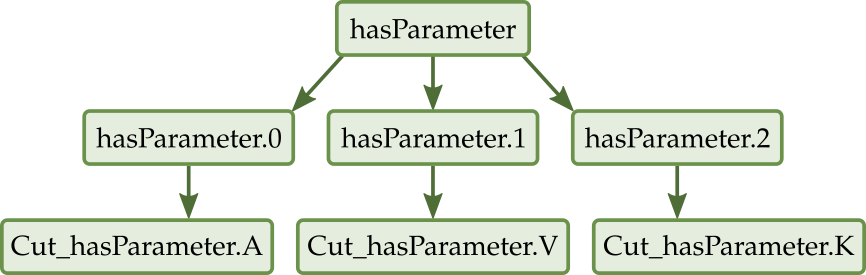
\includegraphics[scale=0.4]{figures/chapter6/rbox_params.png}
\caption{\label{fig:chap6_rbox_params} The properties hierarchy for the parameters of the \textit{Cut} task.}
\end{figure}

Each of these properties is then refined and specified for every task of the \acrshort{htn} to describe. This second specification aims at representing the parameters with their name in the list of task parameters, their position in the parameters list, and the type of entities they can be bounded to. Taking the example of the primitive task \textit{Cut} of Figure~\ref{fig:chap6_domain}, the generated description is presented in Listing~\ref{lst:chap6_owl_params}. The parameter \textit{A} of the \textit{Cut} task is at position 0 of the list of parameters. We thus define the property \textit{Cut\_hasParameter.A} as a refinement of the property \textit{hasParameter.0}. The resulting hierarchy is illustrated on Figure~\ref{fig:chap6_rbox_params} for the parameters of the \textit{Cut} task. The parameter \textit{Cut\_hasParameter.A} aims at representing the agent performing the task. Consequently, the property has to link a \textit{Cut} task to an agent. We represent it respectively with the domain and the range of the property. The same process is performed for every parameter of each task.

\begin{lstlisting}[frame=single, basicstyle=\scriptsize\ttfamily, label={lst:chap6_owl_params}, caption={Description of the \textit{hasParameter} property specifications for the parameters (resp. the agent performing the task, the cut vegetable, and the used knife) of the \textit{Cut} primitive task in the OWL language using the Turtle syntax.},captionpos=b, style=OwlTurtle]
:Cut_hasParameter.A rdf:type owl:ObjectProperty ;
                    rdfs:subPropertyOf :hasParameter.0 ;
                    rdfs:domain :Cut ;
                    rdfs:range :Agent .

:Cut_hasParameter.V rdf:type owl:ObjectProperty ;
                    rdfs:subPropertyOf :hasParameter.1 ;
                    rdfs:domain :Cut ;
                    rdfs:range :Vegetable .

:Cut_hasParameter.K rdf:type owl:ObjectProperty ;
                    rdfs:subPropertyOf :hasParameter.2 ;
                    rdfs:domain :Cut ;
                    rdfs:range :Knife .
\end{lstlisting}

\subsubsection{HET in ontology}

As explained with the gathering scheme, the \acrshort{htn} planner (here \acrshort{hatp}) generates a hierarchical plan for a given human-robot collaborative task that is then executed by the robot and its human partner. Whenever a task (abstract or primitive) is executed by the robot or its execution by the human is perceived, its description is inserted in the agents' KBs. These executed tasks are thus instances of tasks and have to be grounded to the \acrshort{htn} described in the ontology.

\begin{lstlisting}[frame=single, basicstyle=\scriptsize\ttfamily, label={lst:chap6_owl_plan}, caption={A partial description of the initiation of a decomposition of a PrepareVegetable task and its primitive Cut task resulting from a plan and linked to the description of the domain. The description is provided in the OWL language using the Turtle syntax.},captionpos=b, style=OwlTurtle_indiv]
:pv_3 rdf:type owl:NamedIndividual ;
      rdf:type :PrepareVegetable ;
      :hasDecomposition :decomp_pv_3 .

:decomp_pv_3 rdf:type owl:NamedIndividual ;
             rdf:type :PVDecomp_A ;
             :hasSubtask :peel_5 ;
             :hasSubtask :cut_7 .

:cut_7 rdf:type owl:NamedIndividual ;
       rdf:type :Cut_PVDecomp_A ;
       :Cut_hasParameter.A :tony ;
       :Cut_hasParameter.V :c1 ;
       :Cut_hasParameter.K :k2 .
\end{lstlisting}

To explain how the task instances are described in the ontology, let us take the example of an agent executing a decomposition of the abstract task \textit{PrepareVegetable}. A partial representation of this instance is represented in Listing~\ref{lst:chap6_owl_plan} and drawn on Figure~\ref{fig:chap6_abox}.

The human partner has performed \textit{decomp\_pv\_3}, an instance of the decomposition \textit{PVDecomp\_A} being the first decomposition of the abstract task \textit{pv\_3} that is a \textit{PrepareVegetable} abstract task. \textit{pv\_3} is thus an instance of the class \textit{PrepareVegetable} and \textit{decomp\_pv\_3} an instance of the class \textit{PVDecomp\_A}. We use the property \textit{hasDecomposition} to state that \textit{pv\_3} has been achieved with the decomposition \textit{decomp\_pv\_3}. Then, with the property \textit{hasSubtask}, we describe that \textit{decomp\_pv\_3} is composed of two instantiated sub-tasks \textit{peel\_5} and \textit{cut\_7}.

The primitive task \textit{cut\_7} is a \textit{Cut} task but has been achieved in the context of the first decomposition of the abstract task \textit{pv\_3}. The individual \textit{cut\_7} thus inherits of the class  \textit{Cut\_PVDecomp\_A}. Because the \textit{Cut} task has three parameters, they have to be instantiated. To do so, we use the refinements of the property \textit{hasParameter}. Here the task has been performed by the human \textit{tony} who has cut the cucumber \textit{c1} with the knife \textit{k2}. The instance \textit{cut\_7} is linked with \textit{tony} through the property \textit{Cut\_hasParameter.A}, with \textit{c1} the property \textit{Cut\_hasParameter.V}, and with \textit{k2} the property \textit{Cut\_hasParameter.K}. All these instances correspond to the range of each property being respectively an agent, a vegetable, and a knife. The same process should be done for the primitive task \textit{peel\_5}. Moreover, the abstract task \textit{PrepareVegetable} having also three parameters, we should also link \textit{pv\_3} with its instantiated parameters.

\begin{figure}[h!]
\centering
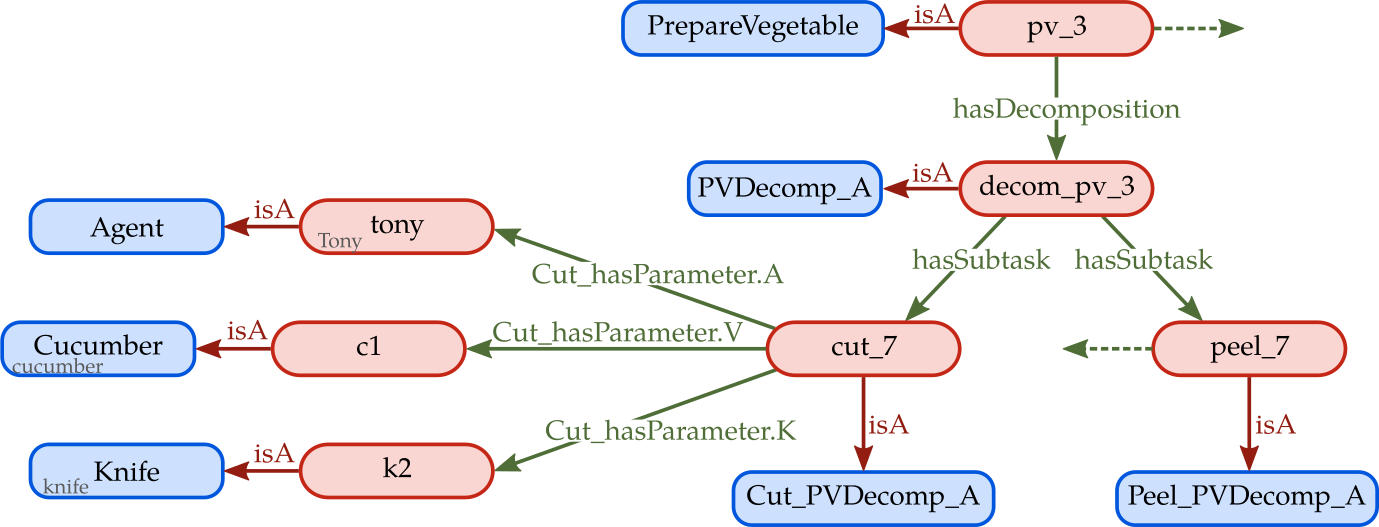
\includegraphics[width=\textwidth]{figures/chapter6/abox.png}
\caption{\label{fig:chap6_abox} A graphical representation of the instance of a decomposition of the abstract task \textit{PrepareVegetable}.}
\end{figure}

\section[REG algorithm modifications]{Modifying the REG algorithm to support the past experiences}

Now the Hierarchical Execution Traces are described in the ontology, we present in this section how we have modified the original \acrfull{ucs} \acrshort{reg} algorithm to make it able to use this new knowledge.

The first assumption we made to use tasks in a \acrshort{reg} solution is that for each task involved in the solution, all its parameters must be part of the solution. This constraint to get all the parameters of a task is important for linguistic realization. If this constraint were not satisfied, we could have results where even the agent having performed the task would not be referred\footnote{This constraint could be an important limitation. It will be discussed in an exploratory work in the next chapter.}.

\begin{theorem} [The complete instantiation]
\label{the:complete_intance}
For any task $\task$ appearing in a \acrshort{re}, all its parameters $\property \in \propset | (\property,\ hasParameter) \in \inclset \wedge (\property, \task) \in \domainset$ must exist in the solution.
\end{theorem}

The $\goaltest$ function which assesses if a node is a goal is modified according to this constraint. In addition to test if $\mathcal{M}(\var_t) = \goalindiv$, it checks if every past tasks used in $\mathcal{T}$ are assigned with all their parameters.

Now we can test if a goal node involves all the parameters of a task, we expand the function finding new actions for the \acrshort{ucs} algorithm. To not confuse the reader between the actions of the \acrshort{ucs} and the actions that a robot can perform, we will rather use the term ``addition'' to speak about relations that can be added to a candidate \acrshort{re} in order to find a solution. We thus adapt the $\additions$ function to explore past tasks and their parameters (Alg.~\ref{alg:chap6_additions}).

\begin{algorithm}[htb!]
\caption{\label{alg:chap6_additions} The modified $\additions$ function with the two newly introduced sub-functions}

\begin{algorithmic}

    \Function{\additions}{$node$} 
        \State $sucess, additions\leftarrow$ \typingadditions($node$)
        \If{$sucess = True\ and\ additions \neq \emptyset$}
            \Return $additions$
        \EndIf
        
        \State $additions\leftarrow$ \completionadditions($node$) \Comment{new introduced function}
        
        \If{$additions \neq \emptyset$}
            \Return $additions$
        \EndIf
        
        \State $additions\leftarrow$ \actingadditions($node$) \Comment{new introduced function}
        \State $additions\leftarrow additions\ \cup$ \differenceadditions($node$) 
        
        \Return $additions$
    \EndFunction
    
\end{algorithmic}
\end{algorithm}

While the $\differenceadditions$ aims at exploring relations that differ from other ambiguous entities, the $\actingadditions$ complements it by exploring the tasks in which the ambiguous entities involved in the candidate \acrshort{re} are part of. In the latter, for each variable $\var_i$ of $\mathcal{M}$ having several substitutions, we search in $\kbs$ all relations involving the anonymous entity $\indiv_i$ and an abtract or primitive task. This means that we are looking at all the relations $\relation = (\indiv_i,\ \property,\ \indiv_{task}) \in \relationset\ |\ (\property,\ isParameterOf) \in \inclset \wedge (\indiv_{task}, HtnTask) \in \inheritset$.

The second added function, $\completionadditions$, aims at making the \acrshort{re} valid. It ensures that any task used in a candidate \acrshort{re} has all its parameters inserted in that \acrshort{re}. For every task $\indiv_{task}$ used in a relation of $\mathcal{T}$ we search in $\relationset$ all the relations having for subject $\indiv_{task}$ and for predicate a property inheriting from $hasParameter$. Among all these relations, the ones not present in $\mathcal{T}$ are added as possible additions of the current node.

Regarding the order in which the addition functions are performed, we always start with the ones aiming to make the candidate \acrshort{re} valid. First, we try to type any anonymous entity. If typing additions have been found or some should have been found but were not, the function stops here. In the case where some have been found, we thus type the anonymous entities. In the other cases, no additions will be generated and the explored branch will be disused. If every anonymous entity is already typed, we try to complete the tasks involved in the candidate \acrshort{re}. If additions have to be done, we stop here and return them. By the way, this means that at the next evaluation of this candidate \acrshort{re}, the newly introduced entity will be typed first before continuing to complete the involved tasks. If every involved task has all its parameters, then and only then, we try to find new actions based on differences or on past tasks.

The cost of an addition representing a task (i.e. an addition involving the property $hasParameter$ or $isParameterOf$) is the cost of the task itself divided by the number of parameters. We chose to process in this way to avoid zero-cost addition and because every inserted parameter will already have a cost due to at least their typing. Thanks to the episodic \acrshort{kb}, the cost of these additions can also be weighted depending on the amount of time passed since the task has been performed. This meets the decay theory used in \cite{williams_2020_toward} and makes a preference over the more recent which could be easier to remember for the \acrshort{re} receiver. The determination of the properties' costs and tasks' costs will not be discussed here but we can mention \cite{belke_2002_tracking} and \cite{koolen_2012_learning} which use learning techniques to estimate them.

Using the presented algorithm, a reference solution to refer to a knife through the primitive task \textit{peel(A,V,K)} of the \acrshort{htn} of Figure~\ref{fig:chap6_domain} could be : \textit{(?0 isA Knife), (?0 isParameterOf ?1), (?1 isA peel), (?1 hasParameter Tony), (?1 hasParameter ?2), (?2 isA Cucumber)}. The variable ?0 represents the referred knife and the variable ?1 represents the task to which the knife is associated. It could be verbalized as \textit{``The knife with which Tony has peeled the cucumber''}.

\section{Results}

We present hereafter the solutions found by our algorithm on an illustrative example and show how the tasks estimated to be known by the \acrshort{re} hearer can impact the algorithm solution. Then, we discuss execution time measures to analyze the impact of such an extension regarding the original version of our \acrshort{ucs}-\acrshort{reg} algorithm.

\subsection{One execution trace for five referring expressions}

Let us take activities of the introduction example where Pr2 and Tony were preparing a meal (Figure~\ref{fig:chap6_intro}). We introduce a third agent, the human Bob, as illustrated in Figure~\ref{fig:chap6_bob}. He is a spectator of the shared activity.

\begin{figure}[ht!]
\centering
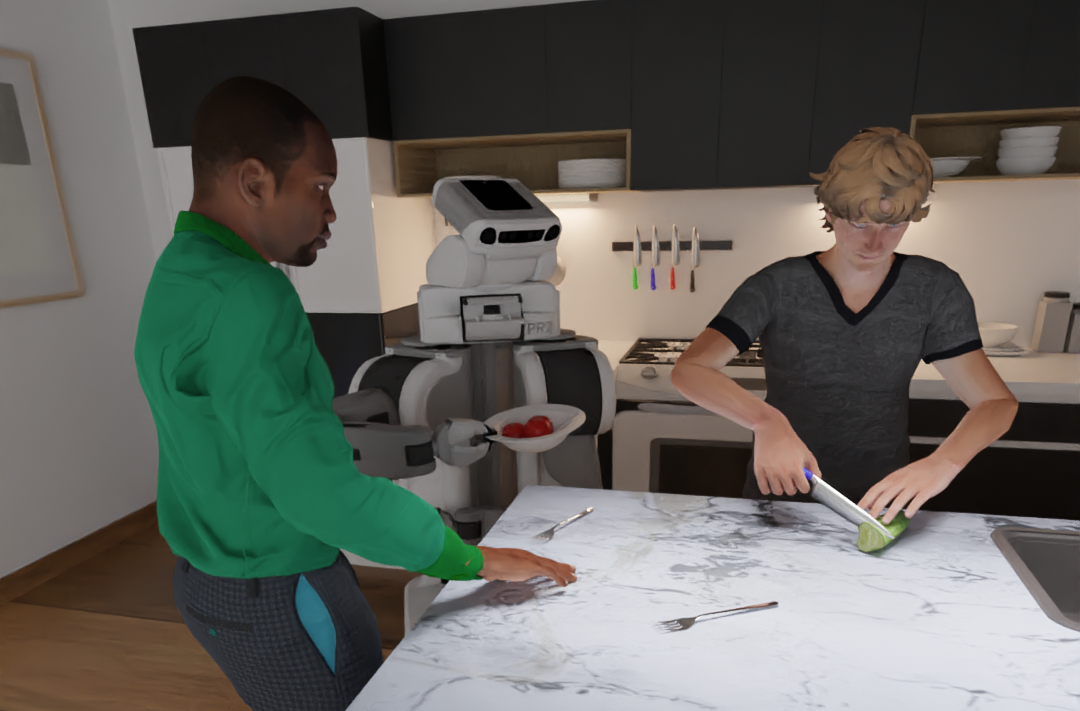
\includegraphics[width=\textwidth]{figures/chapter6/bob.png}
\caption{\label{fig:chap6_bob} A pr2 robot and its human partner Tony, preparing a meal. Bob, a third agent, is looking at them.}
\end{figure}

The shared activity is related to the \acrshort{htn} of Figure~\ref{fig:chap6_domain}. With this \acrshort{htn}, a planner has elaborated a shared hierarchical plan illustrated in Figure~\ref{fig:chap6_meal_plan}. The primitive tasks are listed and organized according to a timeline. The abstract tasks hierarchy is shown on the right. The planner has assigned the tasks to two agents: a robot (pr2) and a human (tony).
 
We define five cases depending on when Bob (the spectator) is in the kitchen where Pr2 and Tony are collaborating for the meal preparation. The colored lines, next to the timeline, represent the moments where Bob is in the kitchen for each case. For example, in case 1 (black line), Bob is only aware of the primitive tasks \textit{Cut(tony,t2,k1)} and \textit{CookSauce(Pr2, t2)}. The primitive tasks the robot estimated Bob to be aware of are thus added to his knowledge bases, both semantic and episodic. Moreover, if an agent is aware of all the tasks (primitive or abstract) composing an abstract task, he is also aware of the abstract task. In the first case, Bob is thus aware of the abstract tasks \textit{PrepareVegetable(tony, t2, k1)},\textit{PrepareVegetableForSauce(tony, k1)}, \textit{CookSauce(pr2)}, and \textit{PrepareSauce()}.

\begin{figure}[ht!]
\centering
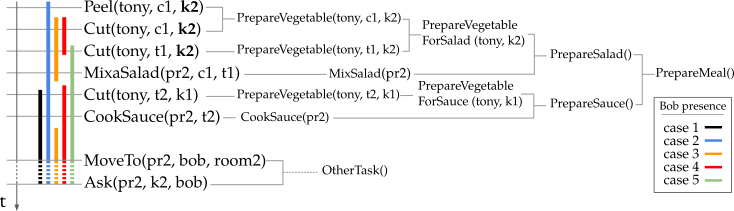
\includegraphics[width=\textwidth]{figures/chapter6/prepare_meal_plan.png}
\caption{\label{fig:chap6_meal_plan} The hierarchical execution trace to prepare the meal and a trace for another subsequent high-level task, organized according to a timeline. In the current instant, PR2 is asking Bob, a second human, for knife \textit{k2}. The five cases are represented by five colors at the left of the tasks and correspond to tasks seen by Bob, the human spectator. In case 1, Bob did not see any tasks involved in the preparation of the salad but was present during the sauce preparation. In the second case, he observed all the activities.}
\end{figure}

In all five cases, the goal is for Pr2 to refer to the knife \textit{k2} to Bob. We assume that the communication about it occurs out of the kitchen. This means that no spatial knowledge is available to generate the \acrshort{re}. We present hereafter the solutions found for each of the cases and detail how they have been found.

\paragraph{Case 1:} The algorithm first types \textit{k2} as being a Knife with the function $\typingadditions$.
Since no task is involved for now in the candidate \acrshort{re}, the $\completionadditions$ does not find any additions. Then, because Bob is not aware of any past task involving \textit{k2}, the $\actingadditions$ does not find addition either. Other relations, such as its color, can be added by the $\differenceadditions$ but none allow to solve the ambiguity. As a result, no solution can be found in this case.

\paragraph{Case 2:} The $\typingadditions$ function first types \textit{k2}. Then, the $\completionadditions$ function has nothing to complete. This time all the tasks (primitive and abstract) performed by Pr2 and Tony are known by Bob. Among them, three primitive tasks and three abstract tasks involve \textit{k2}. The $\actingadditions$ function thus propose six additions of the form $(k2,\ isParameterOf,\ \indiv_t)$ with $\indiv_t$ being the instances of the tasks. The $\differenceadditions$ function has only one possible addition being the color of $k2$. However, it does not help to solve the ambiguity and will give the same solutions as the other candidate \acrshort{re}, with one more relation making it more costly than the others at each step. In the five new nodes to explore involving tasks, the tasks are not labelled and are thus typed. At the next loop, because every candidate \acrshort{re} under exploration involves a task, the $\completionadditions$ function adds one new parameter for each using relation with the $hasParameter$ property. Considering the addition of the agent having performed the tasks, they both have a label and do not need to be typed. Because the abstract task \textit{PrepareVegetableForSalad} has only two parameters while the five others have three parameters, the node exploring it is found to be valid at this step while the others are not. The parameter of the knife has been added by the relation $(k2,\ isParameterOf,\ \indiv_t)$ and the parameter of the agent has been added by the relation $(\indiv_t,\ hasParameter,\ tony)$. The solution \acrshort{re} is: \textit{(?0 isA Knife), (?0 isParameterOf ?1), (?1 isA PrepareVegetableForSalad), (?1 hasParameter tony)}. Matching it in the knowledge base gives only one substitution for the variable ?0 being the target entity \textit{k2}. The verbalization\footnote{The proposed verbalization is automatically generated as proof of usability but the algorithm is not presented here.} would be \textit{``the knife with which Tony prepared the salad vegetables''}.

\paragraph{Case 3:} In this situation, Bob is only aware of two primitive tasks involving \textit{k2} being cutting tasks and one abstract task being a \textit{PrepareVegetable}. Because all have three parameters, at the difference of the previous case, the third parameter of each task is also explored and typed in a second time. At this step, all active nodes are valid. Because all have the same number of parameters, their cost difference depends on the time. The node with the lowest cost is the one with the more recent task. It could be the second cut task of the abstract task of the vegetable preparation. We could prefer the most precise one being the cut task. The solution \acrshort{re} is: \textit{(?0 isA Knife), (?0 isParameterOf ?1), (?1 isA Cut), (?1 hasParameter tony), (?1 hasParameter ?2), (?2 isA tomato)}. Only one substitution exists for the variable ?0 being the target entity. The verbalization would be \textit{``the knife with which Tony cut the tomato''}.

\paragraph{Case 4:} Previously, even if Tony had cut another tomato with another knife, it did not lead to any ambiguity since it was estimated as unknown by Bob. This time, Bob knows that Tony cut two different tomatoes with two knives so the previous solution is not a goal node anymore since two substitutions exist for the variable ?0. The algorithm thus refers to the knife through the cut task on the cucumber \textit{c1}. The verbalization would be \textit{``the knife with which Tony cut the cucumber''}.

\paragraph{Case 5:} In this last case, the only task involving the knife \textit{k2} estimated to be known by Bob is Alex cutting the tomato \textit{t1}. However, Bob knew another cutting task with the tomato \textit{t2} but with the knife \textit{k1} which leads to ambiguity. The algorithm chose anyway the cut task as it is the only possibility. Despite this, our algorithm is able to find a solution by specifying the diverging argument that is the tomato. The tomato \textit{t1} being involved in the \textit{MixSalad} abstract task, the algorithm is able to use this second task to specify the argument of the first one. The solution \acrshort{re} is: \textit{(?0 isA Knife), (?0 isParameterOf ?1), (?1 isA Cut), (?1 hasParameter tony), (?1 hasParameter ?2), (?2 isA tomato), (?2 isParameterOf ?3), (?3 isA MixSalad), (?3 hasParameter pr2), (?3 hasParameter ?4), (?4 isA Cucumber)}. Matching it in the knowledge base gives only one substitution for the variable ?0 being the target entity \textit{k2}. The verbalization would be \textit{``the knife with which Tony cut the tomato that I mixed with the cucumber''}.

Over these five case studies, we saw that the algorithm is able to use either primitive or abstract tasks, to consider the moment where the tasks have been performed to choose the most appropriate one, and to use several tasks in a single \acrshort{re}.

\subsection{The impact of the extension on the performances}

With the previous results, we saw the kind of solution the algorithm can generate. With this new test, we want to assess the impact of the proposed extension, in terms of execution time, regarding the original version. To do so, we have chosen the realistically-sized knowledge base (101 entities, 36 classes, 40 properties, and 497 relations) used to evaluate the original version. For recall, it describes an apartment with three rooms including several pieces of furniture (tables, shelves) and objects (cups, boxes) linked through spatial relations (isAtLeftOf, isOn) and attributes (hasColor, hasWeight). Both the original algorithm and its extended version have been run over all the 77 entities inheriting from the ``Object'' class, representing physical entities. The knowledge base is still managed using the Ontologenius system and we do not pass by the ROS services to not be impacted by the communication time in our measures.

On this ontology, not having tasks described in it, the extension has a negligible impact. The average execution time is about 1.04ms for the original algorithm versus 1.16ms for the extension. Even for the most complex case, we pass from 6.25ms to 6.86ms. This difference can be due to the search of tasks even if none is present in the ontology. Indeed, for each encountered individual, the algorithm has to perform a query to the ontology to check if tasks exist or not.

To estimate the impact when tasks are present in the ontology, we chose to put ourselves in the worst case where tasks are described but can not be used to find a solution. To create this worst case, we add two actions, each having three parameters, to each object described in the apartment. Even if each action is unique (an individual per action), all are of the same type and have the same entities as parameters. In this way, the tasks will be explored but will lead to ambiguity, creating only an overload for the extended algorithm. Consequently, the solutions of both algorithms should be the same. The tasks description leads to an addition of 144 entities to the ontology (the 144 tasks) and 432 relations (three parameters per task). We estimated that such an amount of tasks could be the result of several hours of interaction. With this new setup, the impact of the extension is much more noticeable. For the most complex entity needing six relations in its solution, we pass from 6.40ms to 70.57ms. We note that 75\% of the entities are solved under 5.96ms versus 1.32, 50\% under 1.53ms versus 0.51ms, and 25\% under 0.50ms versus 0.19ms. In addition, we observe that the longer the \acrshort{re} is to compute with the original version, the more noticeable the impact of the extension is. Moreover, because the more relations is needed, the longer the \acrshort{re} is to compute, we find here a part of the explanation. For each node coming from a difference addition (i.e. coming from the function $\differenceadditions$), two additions representing tasks are proposed at the next step. We thus add two to the original branching factor, having an exponential impact on the number of generated nodes and thus on the execution time. However, in an \acrshort{hri} context, even the worst case is still acceptable and will not spoil the interaction. Moreover, we have put ourselves in the worst case where the added tasks can not be used to generate the \acrshort{re}. In more realistic cases, we would have a diversity of tasks and their use in the \acrshort{reg} may allow us to reduce the solution length for the most complex cases and hence reduce the average execution time.

%chap 4
%count    77.000000
%mean      1.080750
%std       1.355236
%min       0.013237
%25%       0.193782
%50%       0.516371
%75%       1.322064
%max       6.405807

%count    77.000000
%mean      5.531283
%std       9.780631
%min       0.012952
%25%       0.509738
%50%       1.538461
%75%       5.968753
%max      70.577606

%2    27
%3    21
%4    14
%5     9
%1     5
%6     1

\section{Discussion}

The contribution presented in this section allows the generation of a new kind of Referring Expression but at the cost of a longer computational time and with the constraint of a precise task description. Moreover, due to the need to use all the parameters of a task, the \acrshort{htn} has to be designed with the goal to be used for \acrshort{reg}.

We can identify three major limitations of the current contribution:
\begin{itemize}
  \item Because we consider the linguistic realization without any consideration of the combination of parameters allowing the generation of a sentence, all the parameters have to be used.
  \item Because the additions consist of the addition of a single relation at a time, all the parameters can not be inserted in a single addition. The consequence is an increase of the branching factor and thus of the execution time.
  \item Because the algorithm search for relations with precise properties in it, the method can not be applied to any task description such as the SOMA~\cite{bessler_2020_foundations} one.
\end{itemize}

These limitations will be discussed in detail in the next chapter through a preliminary work aiming to generalize the Referring Expression Generation that supports the use of past shared tasks.
\ifdefined\included
\else
\setcounter{chapter}{7} %% Numéro du chapitre précédent ;)
\dominitoc
\faketableofcontents
\fi

\chapter{Moving forward binary relations in the REG}
\minitoc
\label{chap:7}

A number of works trend to semantically represent and describe robots' actions and task using ontology. However, each representation has its own particularity, depending on the system it is used on and the exploitation it aims to enable. While our description of past activities fits our needs and our task planner, having a REG algorithm constraint by this latter is problematic. In this chapter we explore the use of n-ary relation, a common, even not yet standard, way to represent complex knowledge as actions. With the analyse of such a pattern, we present a novel REG approach, supporting the use of past activities, but also any complex knowledge represented through n-ary relations.

The contribution presented in this chapter is a preliminary work aiming to consider the limitations encountered by the contribution of the previous chapter. The presented method has been implemented but not tested with an integration with other components. This section deviates a little from the field of \acrshort{hri} to be more anchored in artificial intelligence. However, the ability to generate entity referencing in a more generic way is paramount for a robot to interact with humans. 

\section{Introduction}

Representing the whole complexity of the knowledge composing our world into a machine-readable language is a central issue in artificial intelligence. Coming from the Semantic Web, we saw that the use of an ontology through RDF-based languages succeeded in establishing itself in the field of artificial intelligence and therefore robotics. However, what is often viewed as a limitation of ontology is its capability to only represent unary and binary relations. Binary relations such as \textit{``Sean Connery has the British nationality''} are described through the form of triplets \textit{(sean\_connery, hasNationality, british)}. Unary relation such as \textit{``Sean Connery is an actor''} can them be transformed into binary relation through the addition of dedicated predicates \textit{(sean\_connery, isA, Actor)}. However, the description of more complex relations involving more than two entities is must more challenging using this kind of representation.

Taking the example of Sean Connery\footnote{In the case you do not know who is Sean Connery feel free to take another actor that you like but you will have to adapt the entire example.}, f we want to refer to him\footnote{Obviously we want to refer to him without his name since we consider a person having recognized himself in the previous note.}, we could state that he is the actor playing the role of James Bond. However, other actor played this role. We could also say that he is the actor playing in the film Goldfinger but once again others do. We could finally explain that he is the actor playing the role of James Bond and playing in the film Gold Finger. However, limiting us to the use of binary relations modify the exact information. A more accurate description would be that he is the actor playing the role of James Bond in the film Gold Finger. Here we see the necessity of relations involving more than two entities. In our example, we need to link the three entities that are the actor ``Sean Connery'', the role ``James Bond'', and the film ``Gold Finger''. Together, they describe a performance. Without being explicitly linked, all three theses information would not represent the performance. Moreover, without these links, we could give an explanation such as the actor playing the role of James Bond and playing in the film Rising Sun. Both information is true but does not make sense together.

To refer to an entity, being an object or an agent, such complex relations could be useful but have to be managed carefully to keep the link between each binary relation composing it. In the light of this consideration, we can observe that the description of past agent tasks used in the previous chapter is based on the same principle. Where we refer to Sean Connery through his role and the film he plays in, we have described the knife through the vegetable it has been to cut and the agent having used it. However, depending on the context of the conversation, it is not always necessary to use all the binary relations of such a complex relation. We may need only one. Trying to list the actors having the honorific title of ``Sir'', the referring expression \textit{``The man having played James Bond''} could be sufficient. In the same way, to designate the knife, the sentence \textit{``The knife you cut with''} could also be sufficient in some context.

In this chapter, we will try to generalise the \acrshort{reg} algorithm to deal with non-binary relations and pass over the limitations of the previous chapter. The algorithm has to be more generic and should no more have any apriori of concepts and properties of the used ontology.
First, we review the literature concerning the representation of non-binary relation in ontology. Then, we define what we will call a \acrlong{cr} and how we can represent it. The modified algorithm is then detailed before ending with an efficiency comparison regarding the original version and the extended one.

\section[Related work]{Related work: A richer knowledge representation with n-ary relations}

A fundamental feature of relations is their \textbf{arity}. It is the number of individuals they involved~\cite{giunti_2019_representing}. In this sense, unary relations involved only one entity while binary relation involves two entities\footnote{The entities involved in a relation do not have to be distinct. If the same entity is used twice in the same relation the relation is still a binary relation}. What interest us here is n-ary relations with arity $n > 2$.

Well before being treated for ontology usage, that it is in RDF or OWL, several approaches have been proposed in the field of Artificial Intelligence through the use of semantic network\footnote{Here we close the loop with the hypothesis by Collins and Quillian of the structure of the semantic memory to be like a semantic network.}~\cite{brachman_1979_epistemological, sowa_2014_principles}. Deliyanni and Kowalski~\cite{deliyanni_1979_logic} were the first to explicitly treat the representation of n-ary relations with arity $n > 2$. They propose a semantic network composed of an element representing the relation itself. In this way, they have represented the assertion ``\textit{John gives the book to Mary}'' with five nodes and four arrows as illustrated in figure~\ref{fig:chap7_sem_net}. The central node \textit{el} allows linking the four elements of the assertion using only binary relations. The approach is today know as \textbf{relation reification} and has been used in many applications~\cite{gangemi_2008_norms, welty_2006_reusable}.

\begin{figure}[ht!]
\centering
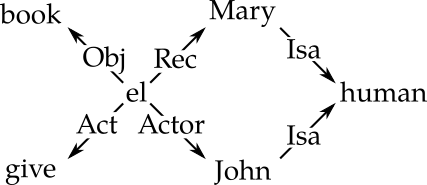
\includegraphics[scale=0.4]{figures/chapter7/semantic_net.png}
\caption{\label{fig:chap7_sem_net} The semantic network used to represent the assertion ``\textit{John gives the book to Mary}''. The element \textit{el} is used to represent the global event.}
\end{figure}

The general idea used in all the proposed approaches since Deliyanni is thus the creation of a \textbf{relation-class} that is instantiated to represent the n-ary relation. Then $n$ binary relations are created to link the $n$ entity to the relation-class instance. For a more global view of the different proposed patterns, you can refer to the survey~\cite{gangemi_2013_multi}.

For the use in ontology, no standard pattern has been approved so far by the W3C. However, a Working Group Note has been proposed for the standardisation of such relations in RDF and OWL~\cite{w3c_2006_defining}. In the note, two patterns are introduced with two variants for the first one.

\begin{figure}[ht!]
\centering
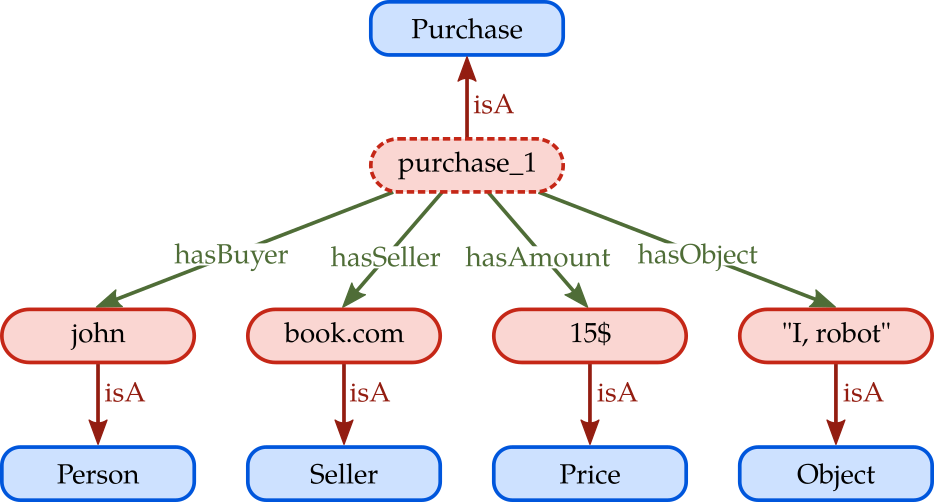
\includegraphics[scale=0.4]{figures/chapter7/w3c_p2.png}
\caption{\label{fig:chap7_w3c_p2} Ontological pattern 1 without subject proposed by the W3C Working Group. The describe assertion is ``John buys ''I, robot`` from books.com for \$15''.}
\end{figure}

The first pattern is based on the introduction of a new class for relation and works in the exact same way as the relation reification as illustrated in figure~\ref{fig:chap7_w3c_p2}. The class \textit{Purchase} is a relation-class and its instance \textit{purchase\_1} is linked to the entities of the relation. Such pattern is said to be \textbf{without subject} as all the relations are oriented from the relation-class instance to the other entities.

\begin{figure}[ht!]
\centering
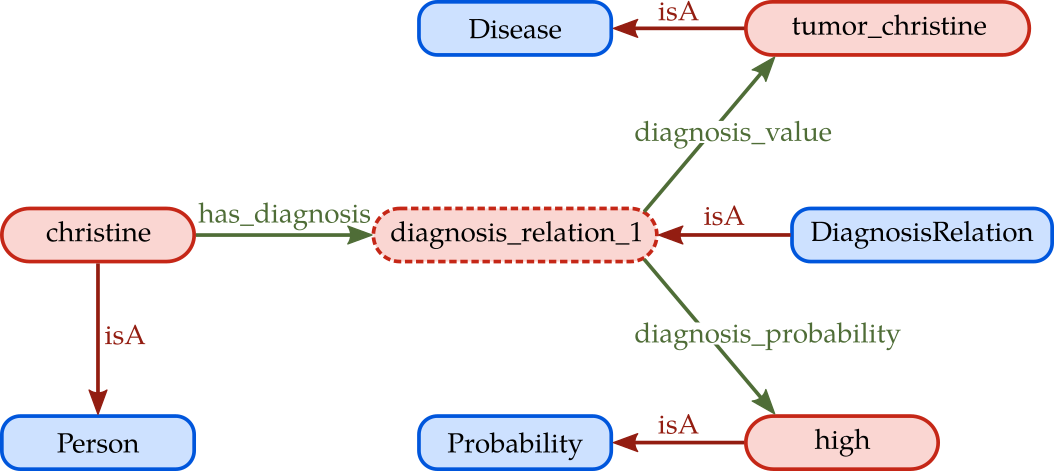
\includegraphics[scale=0.4]{figures/chapter7/w3c_p1.png}
\caption{\label{fig:chap7_w3c_p1} Ontological pattern 1 with subject proposed by the W3C Working Group. The describe assertion is ``Christine has tumor with high probability''.}
\end{figure}


A variation of the first pattern is illustrated in Figure~\ref{fig:chap7_w3c_p1}. This variation is said to be \textbf{with subject}. The assertion described here is ``Christine has a tumor with high probability''. Here the subject of the relation is Christine. It is represented in the pattern by a relation oriented from Christine to the instance of the relation-class while the others are in the usual orientation. Such variation can be reproduced with the previous one by defining inverse relations. Defining the relation \textit{isBuyer} and \textit{isObject}, either John or the book can be the subject of the relation represented by \textit{purchase\_1}.

\begin{figure}[ht!]
\centering
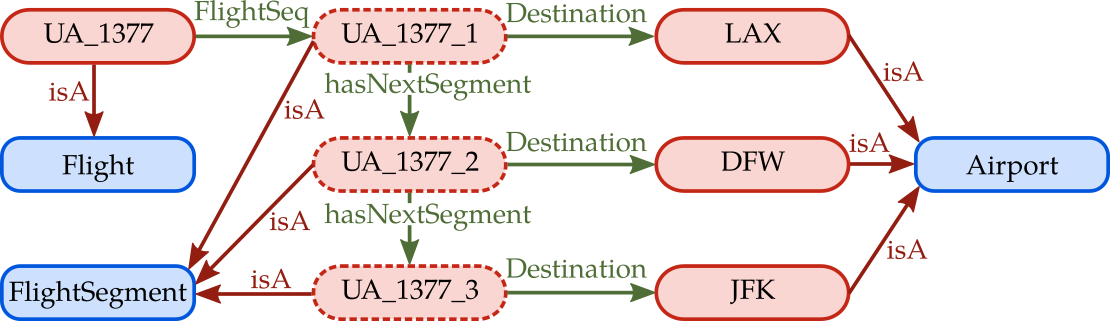
\includegraphics[scale=0.4]{figures/chapter7/w3c_p3.png}
\caption{\label{fig:chap7_w3c_p3} Ontological pattern 2 with subject proposed by the W3C Working Group. The describe assertion is ``United Airlines flight 1377 visits the following airports: LAX, DFW, and JFK''.}
\end{figure}


The second pattern aims at representing lists. With the previous pattern, it is assumed that the properties involved in the binary relation are only used once to identify uniquely each element of the relation. Wanting to represent the assertion ``United Airlines flight 3177 visits the following airports: LAX, DFW, and JFK'' the first pattern would not be adapted. With this other pattern, we create several instances of the relation-class each linked to the next and to an entity of the n-ary relation as illustrated in Figure~\ref{fig:chap7_w3c_p3}. Because one of the binary relations go from an entity of the relation to an instance of the relation-class, it is said to be with subject. This second pattern is dedicated to the description of lists.

\section{Through the use of coumpound relations}

In the rest of the chapter, we consider the n-ary relations with arity $n > 2$ under the name \textbf{\acrfull{cr}} because of the composition of binary relations to represent them on the principle of reification. The term relation will be used to speak about binary relations. We first define what is a \acrshort{cr} in link with the ontology definition and on the base of the first pattern without subject, proposed by the Working Group Note. Then, we present an algorithm to pre-process them with the objective to facilitate their use in the \acrshort{reg} algorithm.

\subsection{Defining a compound relation}

To define the structure of a \acrlong{cr} we take the example of the purchase made by John on the website book.com to buy the book ``I, Robot'' at 15\$, illustrated in figure~\ref{fig:chap7_w3c_p2}. This statement is graphically represented in Fig.~\ref{fig:chap7_cr}a and the underlying pattern in Fig.~\ref{fig:chap7_cr}b. To represent the compound relation, we start by creating a virtual entity (the instance of the relation-class) that will be the common link for all the relations involved in the compound relation. We call this instance entity the \textbf{\acrfull{ce}}. It is the dotted entity on Figure~\ref{fig:chap7_cr}, respectively $purchase\_1$ and $\indiv_c$. We consider as being part of the \acrshort{cr} all the relations for which the \acrshort{ce} is the subject: $(purchase\_1, has\_buyer, john)$. 

\begin{theorem} [Compound Relation]
\label{the:compound_relation}
For any $\indiv_c$ being a Coumpound Entity, a Coumpound Relation is defined by $R_c = \{ \relation_i\ |\  \relation_i = (\indiv_c, \property_i, \indiv_i), \forall \indiv_i \in \indivset\}$ meaning the set of relation composing it.
\end{theorem}

\begin{figure}[ht!]
\centering
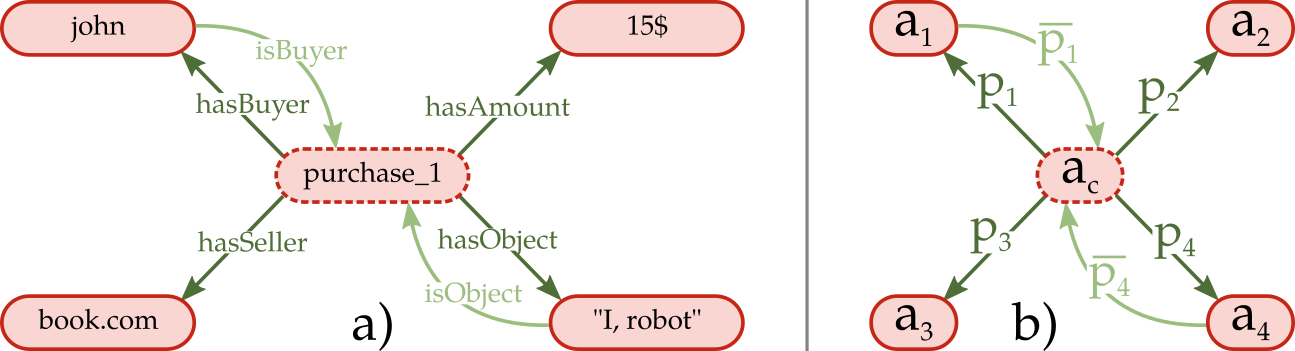
\includegraphics[width=\textwidth]{figures/chapter7/CR.png}
\caption{\label{fig:chap7_cr} The graphical representation of compound relations. The dotted entity at the center of each representation is the so-called compound entity. The outgoing edges are the properties involved in the compound relation. The entering and faded edges are the corresponding inverse properties if any. The compound relation a) describes the purchase made by \underline{John} on the website \underline{book.com} of the book \underline{``I, Robot''} at \underline{15\$}. The compound relation b) is the underlying pattern of the previous example.}
\end{figure}

Regarding the previous definition, because any entity of an ontology could be considered as a \acrshort{ce}, many set of relations without a real link could be considered as a \acrshort{cr}. To solve it, we could define an upper class common to all the \acrshort{ce}, meaning the upper \textit{RelationClass}. However, what better defines a \acrshort{cr} is that to speak about one of its involved entities using the \acrshort{cr}, we have to use other relation of the \acrshort{cr}. In other words, to speak about Sean Connery using the role of James Bond, we have to speak about ``Gold Finger'' rather than ``Murder on the Orient Express'' because even if he played in both films, he played the said role only in the first-mentioned film. Conversely, the relation representing his nationality can be used independently to other relations. To represent this verbal link, Giunti et .al \cite{giunti_2019_representing} introduce a \textit{parametric pattern} on top of n-ary relations (Compound Relations). Their parametric pattern for the purchase example is the following : \textit{``() bought a () from () for ()''}. While as humans we easily identify the place of each entity in the pattern, it is a more complex task for machines. This choice of pattern is explained by their complex representation where they assign a position to each involved relation. Regardless of the representation complexity, this kind of pattern raises two issues. First, the pattern describes the entire \acrshort{cr} and does not aim to describe one of the involved entity through the \acrshort{cr} (e.g. ``\textit{() who bought a () from () for ()}''). Second, the pattern necessarily involves all the relations composing the \acrshort{cr}, while in the context of the \acrshort{reg}, we could only need a part of them (e.g. \textit{``() who bought a ()}'' if John is the only one who bought this book in the present context).

\subsection{A light way of representing the verbal link}

To represent the verbal link, we also choose to use parametric patterns, patterns for short. The patterns are defined as labels in the ontology. A \acrshort{cr} can have multiple labels (i.e. patterns) depending on the subject of the pattern and the involved relations in the verbal link. The labels are not directly applied to the \acrshort{ce} but to a class, it's inheriting. This means that all the entities inheriting from a class having its labels respecting the pattern are \acrshort{ce}. In a way, we define here a relation-class but only through the use of labels.

\begin{theorem} [Compound Entity]
\label{the:compound_entity}
Given $\omega$ being a pattern, an entity $\indiv_c$ is a \acrlong{ce} iif $\exists \class \in \classset | (\indiv_c, \class) \in \inheritset \land \omega \in \tlabel{(\class)}$
\end{theorem}

An advantage of this solution is that we do not define any new specific concepts or properties in the ontology meaning that any pre-existing ontology can be updated to be used in the \acrshort{reg} process with \acrshort{cr} only by adding labels, as n-ary relations are already used. Our patterns have the following form : $\{?\property_4\}\ bought\ on\ \{\property_3\}\ by\ \{\property_1\}$. This pattern directly integrates the properties which can be used to form the relations composing the \acrshort{cr}.

Given a compound entity $a_c$ with the previous label, to generate a referring expression using it, the place-holder $\{\property_3\}$ should be replaced by a referring expression of an entity $\indiv_i$ where $\indiv_i$ is the object of a triple $(\indiv_c,\ \property3,\ \indiv_i)$. Because we assume that a property can only appear once in a \acrshort{cr}, we know that there is only one such object $\indiv_i$. In our example, we have $\indiv_i = \indiv_3$ for the $a_c$ \acrshort{ce}.
In this way, without predefined order, an algorithm can easily replace the place-holders by the \acrshort{re} of the entities $\indiv_i$ of the relations $(\indiv_c, \property_i, \indiv_i)$ of the \acrshort{cr}.

Since we are in the context of \acrshort{reg}, the \acrshort{cr} will be used as a reference to one of the entities involved in it. This specific entity is called the \textbf{subject entity} of the \acrshort{cr}. 
For a subject entity to exist, an inverse property $\overline{\rm \property_i}$ must exist in the way that $(\property_i, \overline{\property_i}) \in \invset$ and $\relation_i = (\indiv_i, \overline{\property_i}, \indiv_c) \in \relationset$. If $\indiv_i$ is the subject entity, $\property_i$ is thus the \textbf{subject property} of the \acrshort{cr} and is prefixed with a question mark in the pattern. In the example of Figure~\ref{fig:chap7_cr}, only $\indiv_1$ and $\indiv_4$ (resp. John and the book) can be subject of the \acrshort{cr}. In other words, only these entities can be referred through the use of this \acrshort{cr}. Among all the labels available to speak about the \acrshort{cr}, the usable ones to speak about an entity are the ones for which the corresponding property is the subject property (i.e. prefixed by a question mark in the patterns). This choice to not consider the first in the pattern has been made to be adapted to any language. Among the possible labels of List.\ref{lst:chap7_john_labels}, the patterns L1 to L5 could thus be used as a reference for $\indiv_4$ (the book in our example) while the patterns L6 and L7 could be used as a reference for $\indiv_1$ (John in our example).

\begin{lstlisting}[frame=single, caption={ A part of the label set of the purchase compound relation.}, label={lst:chap7_john_labels}, captionpos=b, style=Labels, mathescape=true]
L1 - {?$p_4$} bought on {$p_3$} at {$p_2$}
L2 - {?$p_4$} bought by {$p_1$}
L3 - {?$p_4$} bought on {$p_3$} by {$p_1$}
L4 - {$?p_4$} bought at {$p_2$} on {$p_3$} by {$p_1$}
L5 - {$?p_4$} bought at {$p_2$} by {$p_1$}
L6 - {$?p_1$} who bought {$p_4$}
L7 - {$?p_1$} who bought {$p_4$} on {$p_3$}
\end{lstlisting}

\subsection{A strategy to explore compund relations}

In a graph exploration, an important parameter to avoid a combinatorial explosion is the branching factor. For the \acrshort{reg} problem, an advantage of \acrshort{cr} is that once we introduce a \acrshort{cr} in the search algorithm we can directly know the relations involved in it. In this sub-section, our goal is thus to analyze the labels in the way to define the order in which the relations of the \acrshort{cr} will be explored by the upper algorithm. By doing so, we will reduce its branching factor and thus avoid any combinatorial explosion of the \acrshort{reg} algorithm.

\subsubsection{A naive strategy to explore compound relations}

Suppose we want to refer to the entity $\indiv_4$ using the compound relation embodied by the compound entity $\indiv_c$ of Figure~\ref{fig:chap7_cr}. This is made possible by the triplet $(\indiv_c,\property_4,\indiv_4)$ in the knowledge-base and its inverse $(\indiv_4, \overline{\property_4}, \indiv_c)$. The listing~\ref{lst:chap7_john_labels} presents some alternative ways in which we can verbalise entities through the \acrshort{cr}. In order to refer $\indiv_4$, we can only use the ones where $\property_4$ is the subject property. Thus the labels L1 to L5 are the only ones that we can use. The parts of the compound relation used by labels L1 and L3 are illustrated in Figure~\ref{fig:chap7_cr_part}.

\begin{figure}[ht!]
\centering
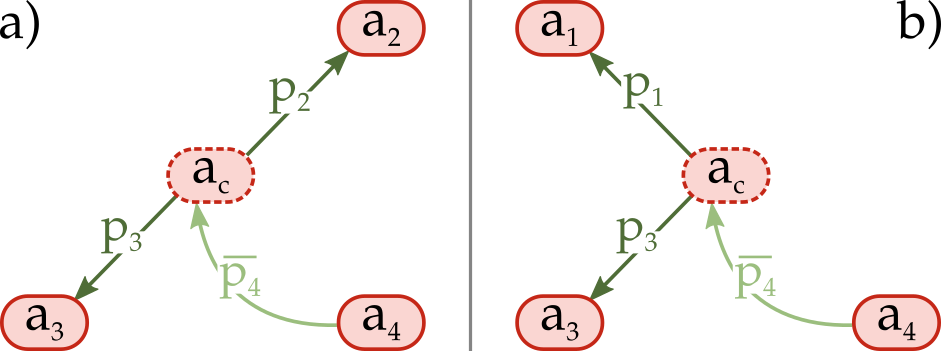
\includegraphics[scale=0.4]{figures/chapter7/CR_part.png}
\caption{\label{fig:chap7_cr_part} The parts of the compound relation used in the label patterns L1 (a) and L3 (b).}
\end{figure}

What interest us in these labels are the involved properties. Indeed, these properties will inform us aboute the realtions to explore. From the patterns in listing~\ref{lst:chap7_john_labels}, we know that we can use label L1 to verbalize the triple set \textit{\{($\indiv_c$,$\property_4$,$\indiv_4$) ($\indiv_c$,$\property_3$,$\indiv_3$) ($\indiv_c$,$\property_2$,$\indiv_2$)\}} and label L2 to verbalise the triple set \textit{\{($\indiv_c$,$\property_4$,$\indiv_4$) ($\indiv_c$,$\property_1$,$\indiv_1$)\}}. On the other hand, other combinations of triplets involving $a_c$ cannot be used to refer to $\indiv_4$. Therefore, we can see each label usable to refer $\indiv_4$ as a set of properties and the collection of usable labels as a family of sets. In our example, the family of sets over S is the collection:

\begin{align*}
 F\ =\ \{\{p_2\ p_3\ p_4\},
\{p_1\ p_4\},
\{p_1\ p_3\ p_4\},
\{p_1\ p_2\ p_3\ p_4\},
\{p_1\ p_2\ p_4\}\}
\end{align*}

From there, our goal is to create a search-tree that will conduct the exploration of the different labels of a \acrshort{cr} through the exploration of the properties composing them. This search-tree has few constraints:
\begin{enumerate}
	\item The tree must be composed of a single root.
	\item All the descendants of a node have a common prefix of the property associated with that node. In this way, the search-tree is more precisely a trie, also called prefix tree.
	\item Walking through the tree from its root, we recompose all the subsets of the family $F$.
	\item The width of the tree must be as small as possible.
\end{enumerate}

A naive solution not minimizing the width of the tree is represented in Figure~\ref{fig:chap7_naive}a) for the purchase example. We consider the root $\property_4$ and create a branch per label. The resulting width is five. On the Figure~\ref{fig:chap7_naive}b) we merge the node representing the same property at an equivalent level. It reduces the branching factor for the beginning of the exploration by the global width is the same. Switching the elements $p_2$ and $p_3$ for L4 and keeping the merging principle, we can see in Figure~\ref{fig:chap7_naive}c) that the width of the trie can be reduced to four. An advanced algorithm to build the graph could thus reduce the width of the trie.

\begin{figure}[ht!]
\centering
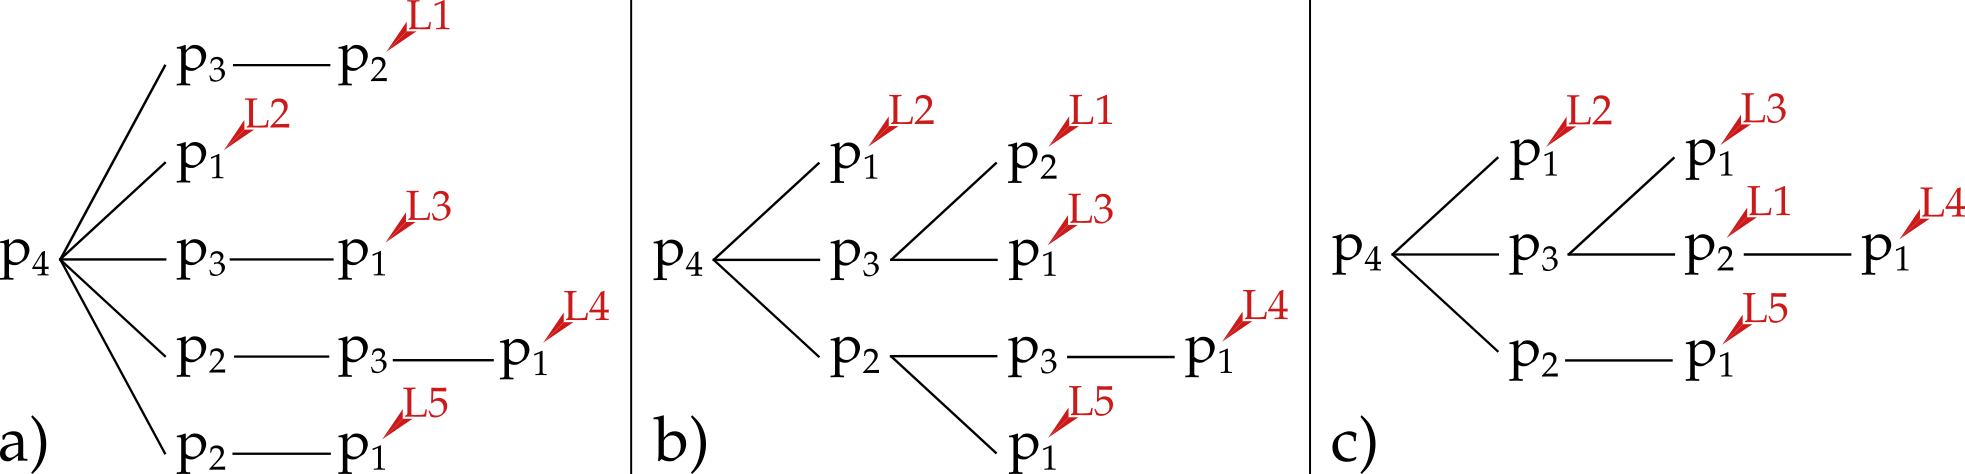
\includegraphics[width=\textwidth]{figures/chapter7/naive.png}
\caption{\label{fig:chap7_naive} Two naive trie representations of the family of subsets extracted from properties involved in the label patterns. The trie a) considers the subject property as the root of the tree and creates a branch for each label pattern respecting the order of apparition of the properties. The trie b) takes the same construction rule as the a) but merges the common children of each node. The trie c) is the same principle of b) but the elements $p_2$ and $p_3$ have been switched for L4. While the two first tries have a width of five, the last has a width of four.}
\end{figure}

\subsubsection{Advanced strategy to explore compound relations}

To find a strategy to create a trie minimizing the width, we first have to study the characteristics of the family of sets.
The first axiom that we can do on the subsets of our family is that they are neither totally ordered, as we can explore their element in any order, or partially ordered, as we can not compare their members. Therefore, we cannot use the tools of the order theory such as the Hasse diagram. Taking a look at mathematical approaches of tree-representation of set families~\cite{bui_2008_tree}, we face the problem that our set family does not respect some essential properties. For each pair $(A, B)$ of sets of $S$, we can not ensure that one of the following rules is true : $A \cap B \neq \emptyset$, $A \cap B \neq A$, or $A \cap B \neq B$. This means that we cannot ensure that each pair of sets are either disjoint or related by containment. Wherefore, our family $F$ is not a laminar set family.
Moreover, for each pair $(A, B)$ of sets of $S$, we can not ensure that their intersection is non-empty ($A \cap B \neq \emptyset$), neither that their differences are non-empty ($A \setminus B \neq \emptyset$ and $B \setminus A \neq \emptyset$). Wherefore, our family $F$ is not a cross-free or an overlap-free family but it does not mean that it is an intersecting and crossing family.

To limit our problem, we do a first assumption. Because the subject property $\property_s$ is the one having introduced the \acrshort{cr}, we can assume that this property has already been selected among the others. Moreover, it will always be the common element of all the sets of the family. We thus consider it as the root node of the exploration tree and remove it from every set of the family $S$ giving a new family:

\begin{align*}
S' = \{A\ |\ A = X \setminus \property_s,\ \forall X \subseteq S\}
\end{align*}

From there, we need to find the child nodes of the root in a way to minimize their number and that every subset of $S'$ has at least one of their element attached to one of the child nodes. This sub-problem is a specification of the Hitting Set problem. It is defined as follows. Giving $F = \{S_1,S_2,...,S_m\}$ the collection of subsets of $S$ (i.e. $S_i \subseteq S, \forall i$) and a natural number $k \in \field{N}$, we want to know if exists $S' \subset S$ where $|S'| < k$ such that $S_i \cap S' \neq \emptyset, i = 1,2,...,m$. In our case, we are searching $k$ as to be as small as possible. In some way, the Hitting Set problem can be seen as a Set Covering problem, shown to be NP-complete~\cite{karp_1972_reducibility}. To avoid any combinatorial explosions, we thus propose a greedy algorithm.

Given a node $n_i$ of the tree and its related family of set $S$, the quantity $|\{S_j \in S ~|~ x_i \in S_j \}|$ is the frequency of the element $x_i$ in $S$. Among the elements of the universe of the current node $n$, we select $x_{max}$, the element with the highest frequency and create a child node with it. The family related to this new node is computed with the equation~\eqref{eq:chap7_child_family} and the family related to the current node is updated with the equation~\eqref{eq:chap7_node_family_update}. These steps are repeated while $S$ is non-empty to create all the children of the current node and this process is repeated for each created child nodes until it is possible.

\begin{equation}
S' = \{S_j \setminus x_{max}, S_j \cap \{x_{max}\} \neq \emptyset, \forall S_j \in S\}
\label{eq:chap7_child_family}
\end{equation}

\begin{equation}
S \leftarrow \{S_j, S_j \cap \{x_{max}\} = \emptyset, \forall S_j \in S\}
\label{eq:chap7_node_family_update}
\end{equation}

The tree resulting from this process is represented in Figure~\ref{fig:chap7_advanced} for the purchase example. In the root node with the property $p_4$, the element with the highest frequency is $p_1$. We thus create a child node with this property and create its family. Updating the family of the root node, the family only contains the set $\{p_2, p_3\}$. Both having the same frequency, one is chosen over the other, here $p_3$, and we create a new child node. After an update of the family of the root, it will be empty and all the children of the root have been created. The process is repeated for the two created nodes.

\begin{figure}[ht!]
\centering
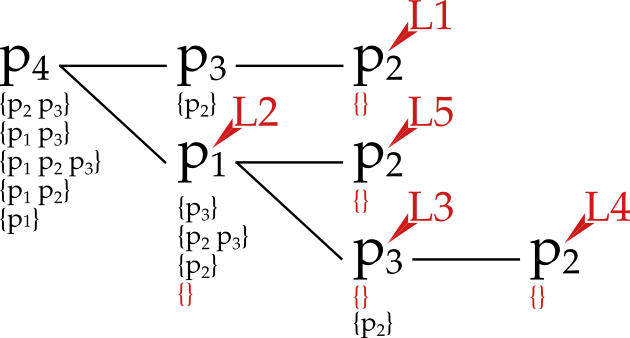
\includegraphics[scale=0.45]{figures/chapter7/advanced.png}
\caption{\label{fig:chap7_advanced} The trie with reduced width, representing all the labels of a compound entity in terms of involved properties. Each node is a property to explore. Attached to each node is the family of subsets that has to be decomposed. An empty set in a family related to a node (in red) signified that one of the initial subsets is fully represented in the trie, meaning that all the properties of a pattern will be explored by reaching this node. The width of the trie is three against five for the naive version.}
\end{figure}

In the following, such search-tree will be referred to as a \acrfull{ct}. Taking a part of it (i.e. taking one of its nodes as a local root) gives a sub-\acrshort{ct}.

\section{REG with compound relations}

Thanks to the \acrshort{ce} labels analysis, we have created a search-tree to lead the exploration of \acrshort{cr} in the \acrshort{reg} algorithm. In this section, we present the modification we made to use \acrshort{cr} in the \acrshort{reg} algorithm. The core of the algorithm based on the Uniform Cost Search algorithm is unchanged and is recalled in algorithm~\ref{alg:chap7_ucs}.

\begin{algorithm}[!ht]
\caption{Uniform-Cost Search algorithm for Referring Expression Generation}
\label{alg:chap7_ucs}
\begin{algorithmic}
\Function{UCS\_REG}{$problem$} 
    \State $node\leftarrow$ a node with RE = \textsc{create-initial-re}(\textit{problem}.context), \textit{cost} = 0
    \State $frontier\leftarrow$ a priority queue of nodes ordered by their \textit{cost}
    \State $frontier\leftarrow$ \textsc{INSERT}($node$, $frontier$)
    \State $explored\leftarrow$ an empty set
    \Loop
        \If{\textsc{empty}($frontier$)} 
        	\State \Return failure
        \EndIf
        \State $node\leftarrow$ \textsc{pop}($frontier$)
        \If{\goaltest($problem$, \toquery($node$))} 
        	\State \Return \textsc{SOLUTION}($node$)
        \EndIf
        \State add $node.RE$ to $explored$
        \ForAll{$addition$ in \additions($node$)}
            \State $child \leftarrow \createchild(node, addition)$
            \If{$child.RE$ is not in $explored$ or $frontier$}
            	\State $frontier\leftarrow$ \textsc{INSERT}($child$, $frontier$)
            \EndIf
        \EndFor
    \EndLoop
\EndFunction
\end{algorithmic}
\end{algorithm}

\subsection{Exploring the compound relations}

At the difference of the tasks descriptions of the previous chapter, the current algorithm can not have any prior knowledge about the relations leading to the use of \acrshort{cr}. A \acrshort{cr} can only be discovered if a relation introduces a \acrshort{ce}. However, an entity can be said to be a \acrshort{ce} only thanks to the labels of one of its upper class. With regard to this information, we cannot have any function dedicated to the addition of \acrshort{cr} and each newly introduced entity in a candidate \acrshort{re} has to be tested to assess if it is a \acrshort{ce} or not.

The analysis of the entities' labels and their usable classes, meaning their upper classes having labels, is an already existing process in the \acrshort{reg} algorithm. It is performed by the function $\typingadditions$ of algorithm~\ref{alg:typing_action}. It initially aims at satisfying the parlance need constraint (theorem~\ref{the:parlance_need}). With some modifications, the $\typingadditions$ will be used to detect any newly introduced \acrshort{ce} by testing if the labels of the usable classes are in the form of a pattern. If they are, it returns the detected \acrshort{ce}. To do so, the \textit{additions} are now composed of a relation to be added and a \acrshort{ce} if one has been found.

Once \acrshort{ce}s have been detected, we have to create a \acrfull{ct} for each one in order to lead the \acrshort{reg} search process. To each node of the \acrshort{reg} algorithm, in addition to the candidate \acrshort{re} and its associated cost, we introduce a map of \acrshort{ct}s. This map link a \acrshort{ce} involves in the candidate \acrshort{re} related to the node to its \acrshort{ct} or one of its sub-\acrshort{ct}. The management of these trees is done by the $\createchild$ that has been modified (see algorithm~\ref{alg:chap7_child}). If the addition introduces a new \acrshort{ce}, we create its related \acrshort{ct}\footnote{For performance gain, all created \acrshort{ct} can be stored in a collection of \acrshort{ct} in order to compute them only once even if the same \acrshort{ce} is introduced in two disting branches of the \acrshort{ucs}.}. Otherwise, with the function $\getsubtrees$ we test if the new relation corresponds to one of the branches of one of the \acrshort{ct}s of the parent node. If it is, we take the sub-\acrshort{ct} corresponding to the relation. Taking the entity $\indiv_c$ as introduced \acrshort{ce} through the relation $(\indiv_4, \overline{\property_4}, \indiv_c)$, the \acrshort{ct} of figure~\ref{fig:chap7_advanced} is first created. If in a second time the relation $(\indiv_c, \property_1, \indiv_1)$ is inserted, $\createchild$ would take the sub-\acrshort{ct} having $\property_1$ as root.

\begin{algorithm}[ht!]
\caption{\label{alg:chap7_child} Child node function modified to use compound relations.}
\begin{algorithmic}
\Function{\createchild}{$addition$, $parent$} 
    \State \Return a node with
    \State RE = $parent$.RE $\cup$ $addition$.relation
    \State cost = $parent$.cost + $\costfunc(addition$.relation$)$
    \If{$addition$.CE}
    	\State CTs $\leftarrow$ INSERT($\createtree(addition$.CE$)$, $parent$.CTs)
    \Else
    	\State CTs $\leftarrow$ $\getsubtrees$($addition$.relation, $parent$.CTs)
    \EndIf
\EndFunction
\end{algorithmic}
\end{algorithm}

At this stage, we detect the introduction of \acrshort{cr} and manage the \acrshort{ct}s. The $\additions$ can now use the \acrshort{ct}s to propose new additions. As describe with the algorithm~\ref{alg:chap7_additions}, we keep the two functions $typingadditions$ and $\differenceadditions$. We introduce a new function $\compoundadditions$ aiming to complete the \acrshort{cr} having been started. For each \acrshort{ct} of the node, it proposes the relation of the form $(\indiv_c, \property_i, \indiv_i) \in \relationset$ such that the properties $\property_i$ are the branches of the root of the \acrshort{ct} related to $\indiv_c$. With the  \acrshort{ct} of figure~\ref{fig:chap7_advanced}, the $\compoundadditions$ function would generate two addtions being $(\indiv_c, \property_3, \indiv_3)$ and $(\indiv_c, \property_1, \indiv_1)$.

\begin{algorithm}[ht!]
\caption{\label{alg:chap7_additions} The modified $\additions$ function modified to use compound relations. }

\begin{algorithmic}

    \Function{\additions}{$node$} 
        \State $sucess, additions\leftarrow$ \typingadditions($node$)
        \If{$sucess = True\ and\ additions \neq \emptyset$}
            \Return $additions$
        \EndIf
        
        \State $additions\leftarrow$ \compoundadditions($node$) \Comment{new introduced function}
        \State $additions\leftarrow additions\ \cup$ \differenceadditions($node$) 
        
        \Return $additions$
    \EndFunction
    
\end{algorithmic}
\end{algorithm}

\subsection{Determining a referring expression validity}

Going back to the original definition of the \acrshort{reg} problem, a \acrshort{re} is valid if the parlance need is satisfied (theorem~\ref{the:parlance_need}), all the introduced variables can be intantiated (theorem~\ref{the:correct_intance}), and the variable representing the target entity can only be bound to the target entity (theorem~\ref{the:re_mini_validity}) for a minimal validity.

For the compound relations, their validity criteria is that we can use one of their labels to speak about them. In other words, taking all the relations involving a given \acrshort{ce}, we must be able to rebuild one of its family's sets. Each of its \acrshort{cr} thus has to be complete (see theorem~\ref{the:cd_completion}).

\begin{theorem} [The CR completion]
\label{the:cd_completion}
A \acrshort{cr} of family $S$ is said to be complet iif given its \acrshort{ce} $\indiv_c$ we can create, from the set of relation $\mathcal{T}$ representing a candidate \acrshort{re}, a set $v = \{\property_i\ |\ (\indiv_c, \property_i, \indiv_i) \in \mathcal{T} \lor (\indiv_i, \overline{\property_i}, \indiv_c) \in \mathcal{T} \}$ such that $v \subset S$.
\end{theorem}

From a technical point of view, such constraint can be hard to compute for each node to be tested. However, during the creation of a \acrshort{ct}, this information can already be known. During the \acrshort{ct} creation, each time a child node is created with an empty set its family of sets, this means that a label of the \acrshort{cr} is represented in its entirety at this node. In the figure~\ref{fig:chap7_advanced}, the completed labels are represented by the red arrows. We can thus store this information in the \acrshort{ct} nodes. Because during the \acrshort{reg} search process we cut down these trees taking each time a sub-\acrshort{ct}, we just have to test if each current root of the \acrshort{ct}s of the node to test can represent a label or not. If all of them can, the candidate \acrshort{re} of the current node is valid regarding the \acrshort{cr} completion.

\subsection{From tree to radix tree}

A limitation identified from the previous chapter was the addition of a single relation at each step while we can know that the candidate \acrshort{re} will not be valid because of the completion constraint. With the present method using multiple labels not involving all the relations, the limitation has been partially solved. In addition, thanks to the \acrshort{ct}, the branching factor is limited and even if an addition does not lead to a valid \acrshort{re}, it will be used for several labels. However, in some cases, this limitation still appears. Considering the \acrlong{ct} of figure~\ref{fig:chap7_advanced}, starting from the root node $\property_4$, we can go to the nodes $\property_3$ and $\property_1$. While the node $\property_1$ creates a complete \acrshort{cr} and makes a step toward another complete \acrshort{cr}, the node $\property_3$ does not. It makes a step toward the single label $L1$ but does not complete it.

To solve this issue, we can use the radix tree structure, also called compact prefix tree. It consists of merging each node that is the only child with its parent if the parent node does not represent a valid label. In the example of figure~\ref{fig:chap7_advanced}, the node with the property $\property_2$ could thus be merged with its parent $\property_3$.

The major consequence of such modification is that the additions have to no more represent a single relation but a set of relations. Even if it makes the additions comparison harder to compute it reduces the overall branching factor. Keeping our example, if we add at once the relation involving $\property_2$ and $\property_3$ and that both introduce an anonymous entity, this means that at the next step the $\typingadditions$ function could type both in one step. Where previously these additions would require four steps, and thus branching at each, with this solution it only requires two.

\section{Results}

In this section, we present some results of the \acrshort{reg} with compound relations. We start with the introduction example of Sean Connery's performance. Then we give performance measures using the setup of the previous chapter in order to assess the impact of the proposed modifications. 

\subsection{The actor playing James Bond}

For this simple test, we describe actor performance using the pattern of figure~\ref{fig:chap7_perf}. Both the actor and the film can be used as a subject of the \acrshort{cr} thanks to the presence of inverse properties. The set of labels attached to the \textit{Performance} class is listed in listing~\ref{lst:chap7_perf_labels}. Three are available to describe the actor and two (equivalent) for the film.

\begin{figure}[ht!]
\centering
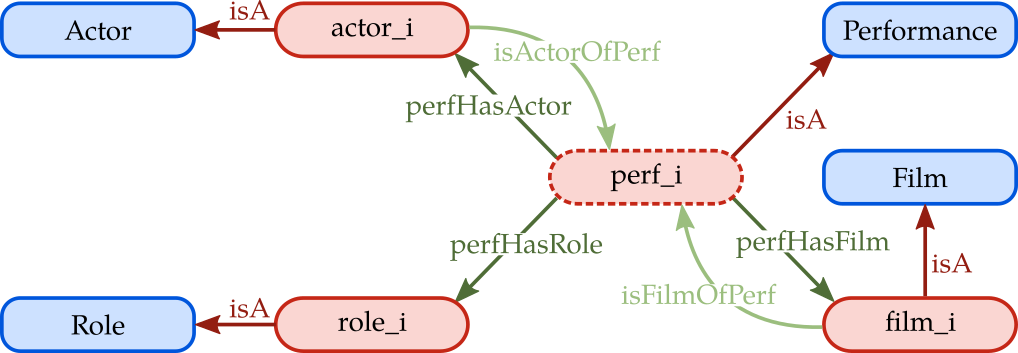
\includegraphics[scale=0.4]{figures/chapter7/perf.png}
\caption{\label{fig:chap7_perf} The compound relation pattern used to describe a performance of an actor with a role and a film.}
\end{figure}

\begin{lstlisting}[frame=single, caption={ The set of labels usable to discribe the performance compound relation.}, label={lst:chap7_perf_labels}, captionpos=b, style=Labels, mathescape=true]
L1 - {?perfHasActor} who played {perfHasRole} in {perfHasFilm}
L2 - {?perfHasActor} who played {perfHasRole}
L3 - {?perfHasActor} who played in {perfHasFilm}
L4 - {?perfHasFilm} in which {perfHasActor} play {perfHasRole}
L5 - {?perfHasFilm} in which {perfHasRole} is played by {perfHasActor}
\end{lstlisting}

We first create an ontology describing two performances. The performance \textit{perf\_sean} link the actor \textit{sean\_connery} with the role of \textit{james\_bond} and the film \textit{gold\_finger}. The second is \textit{perf\_craig} with \textit{daniel\_craig} in the role of \textit{james\_bond} and in the film \textit{casino\_royale}. The individuals representing the films and the roles have labels while the others do not. Running our algorithm on this ontology we get the result:

\begin{gather*}
(?0,\ isA,\ Actor),\\
(?0,\ isActorOfPerf,\ ?1),\\
(?1,\ isA,\ Performance),\\
(?1,\ perfHasFilm,\ gold\_finger)
\end{gather*}

Matching it in the ontology, the variable \textit{?0} matchs \textit{sean\_connery} and the variable \textit{?1} matchs the performance \textit{perf\_sean}. Adding the performance \textit{perf\_gert} linking the actor \textit{gert\_frobe} with the role of \textit{auric\_finger} and the film \textit{gold\_finger} the previous solution is no more valid. Running the algorithm on the new ontology, we get the result:

\begin{gather*}
(?0,\ isA,\ Actor),\\
(?0,\ isActorOfPerf,\ ?1),\\
(?1,\ isA,\ Performance),\\
(?1,\ perfHasFilm,\ gold\_finger),\\
(?1,\ perfHasRole,\ james\_bond)
\end{gather*}

With this simple example we see that with a single compound relation, the algorithm is able to find a solution by selecting the necessary information in it depending on the situation, while keeping the link between each of them.

\subsection{The description of past activities as compound relations}

From now, we see that \acrlong{cr} can be used to represent complex knowledge with various entities linked together. Considering now the representation of an agent's past activities, presented in the previous chapter, such a complex knowledge could thus be represented using \acrshort{cr}s. Figure~\ref{fig:chap6_abox} represented a part of an ABox of an instance of a decomposition of the abstract task \textit{PrepareVegetable}. Focusing on the primitive task \textit{Cut} and its instance \textit{cut\_7}, we can observe that the underlying pattern already was a \acrshort{cr}. The graphical representation of this description is reported in figure~\ref{fig:chap7_cut7}.

\begin{figure}[ht!]
\centering
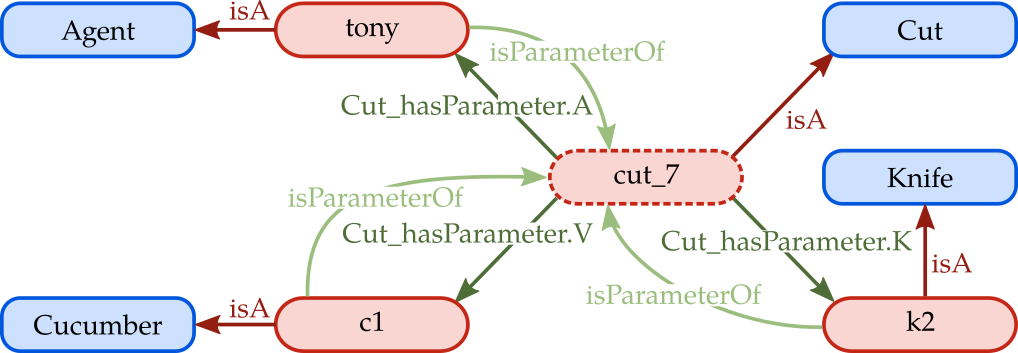
\includegraphics[scale=0.4]{figures/chapter7/cut7.png}
\caption{\label{fig:chap7_cut7} The underlined \acrlong{cr} pattern used to discribe a past activity. The entity \textit{cut\_7} can thus be considered as a \acrlong{ce}. }
\end{figure}

At the light of the presentation of the \acrshort{cr}, we see that the entity \textit{cut\_7} is the \acrlong{ce} of the \acrlong{cr} and that the class \textit{Cut} is a relation class. Moreover, due to the presence of the inverse property \textit{isParameterOf}, common to all the used properties, the three involved entities could be used as a subject entity. The only element to add to the previous representation is the labels, in the form of patterns. For the cut task, the proposed labels are listed in the listing~\ref{lst:chap7_cut_labels}. Among these labels, we see that for all the possible subject entities, two labels are available, involving one or two additional entities.

\begin{lstlisting}[frame=single, caption={ The set of labels usable to discribe the compound relation representing an instance of a cut primitive task.}, label={lst:chap7_cut_labels}, captionpos=b, style=Labels, mathescape=true]
L1 - {?Cut_hasParameter.A} who cut {Cut_hasParameter.V}
L2 - {?Cut_hasParameter.A} who cut {Cut_hasParameter.V} 
     with {Cut_hasParameter.K}
L3 - {?Cut_hasParameter.V} cut by {Cut_hasParameter.A}
L4 - {?Cut_hasParameter.V} cut by {Cut_hasParameter.A} 
     with {Cut_hasParameter.K}
L5 - {?Cut_hasParameter.K} with which {Cut_hasParameter.A} cut
L6 - {?Cut_hasParameter.K} with which {Cut_hasParameter.A} cut 
     {Cut_hasParameter.V}
\end{lstlisting}

To assess the utility to consider the past activities representation as \acrlong{cr}, we take again the execution trace of figure~\ref{fig:chap6_meal_plan} and propose three new cases. The trace and the new cases are illustrated in figure~\ref{fig:chap7_meal_plan}. As a reminder, the plan was executed by two agents, Tony, a human, and Pr2, a robot. A third agent, Bob, see part of the execution. Each case corresponds to a set of task, seen and thus known by Bob. The goal here is still to refer to the knife \textit{k2}. The usable labels are thus L5 and L6, both referring to the knife used in the task.

\begin{figure}[ht!]
\centering
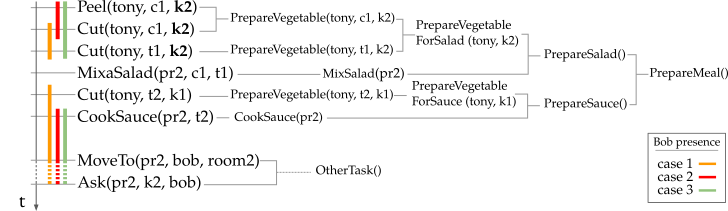
\includegraphics[width=\textwidth]{figures/chapter7/prepare_meal_plan.png}
\caption{\label{fig:chap7_meal_plan} The hierarchical execution trace to prepare the meal and a trace for another subsequent high-level task, organized according to a timeline. In the current instant, PR2 is asking Bob, a second human, for knife \textit{k2}. The three cases are represented by three colors at the left of the tasks and correspond to tasks seen by Bob, the human spectator.}
\end{figure}

\paragraph{Case 1:} Bob only saw two tasks involving the knife \textit{k2}. Both are cut task but on different vegetables. The algorithm can try to use the label L5, being shorter than L6. However, both tasks have been achieved by Tony. Consequently, the algorithm selects a \acrshort{re} using L6. The solution \acrshort{re} is: \textit{(?0 isA Knife), (?0 isParameterOf ?1), (?1 isA Cut), (?1 Cut\_hasParameter.A tony), (?1 Cut\_hasParameter.V ?2), (?2 isA tomato)}. The algorithm not based on \acrshort{cr}, would have give the same solution. The only difference is in its form. Here, the triplets representing the parameter use the properties really used to describe the \acrshort{cr}, where the previous algorithm would have used the more abstract property \textit{hasParameter}.

\paragraph{Case 2:} In the second case, Bob only saw two tasks involving the knife \textit{k2}. This time, it is two different tasks as one is a cutting task while the other is a peeling task. In this situation, the algorithm can use the label L5 and provide the solution: \textit{(?0 isA Knife), (?0 isParameterOf ?1), (?1 isA Cut), (?1 Cut\_hasParameter.A tony)}. We note that the cut vegetable is not present in the solution since it does not provide discriminative information. Bob saw Tony cut only a cucumber so specifying the vegetable would be useless. The algorithm not based on \acrshort{cr} would have provided all the parameters, even if some are useless. The \acrshort{cr}-based algorithm is thus able to find shorter \acrshort{re} when the current situation allows it.

\paragraph{Case 3:} In the third case, Bob saw three tasks. Two of them are cutting task while the other is a peeling task. Even if one of these tasks is different from the others, for the previous algorithm all of them involved three parameters. Consequently, they would have had all the same cost. The selection would have been based on the time, selecting the most recent one. For the \acrshort{cr}-based algorithm, the two cutting tasks need all of their parameters to be referred to but the peeling task can be used without reference to the peeled vegetable. Using the latter task allows to generate a shorter \acrshort{re}. Considering the peel task as having the same kind of labels than the cut task, the final solution \acrshort{re} is: \textit{(?0 isA Knife), (?0 isParameterOf ?1), (?1 isA Peel), (?1 Peel\_hasParameter.A tony)}.

Over these three cases, we saw the \acrshort{cr}-based algorithm is suitable to be used with descriptions of past activities. The advantage of this algorithm regarding the previously made is the form of the generated \acrshort{re} with the use of precise properties, and the ability to generate shorter \acrshort{re} in some situations. The most important point is that the algorithm is less dependant on the knowledge representation. It does not need priory about the properties of the representation. By simple adding labels to existing representation, the current algorithm can be used with other task representations.

Finally, even if we will not illustrate it, the use of \acrshort{cr} to represent past activities could allow us to be restricted by the information provided by a task planned. Taking the example of the cut task, it is performed on a support, a work plan. Even if this piece of information is not necessarily provided by a task planner, when the task is performed, the work plan on which the task is performed can be perceived by the robot. This additional information could be used to generate \acrshort{re}. To support this new information, we could add a label L7:

\begin{quote} 
\centering 
\{?Cut\_hasParameter.K\} with which \{Cut\_hasParameter.A\} cut on \{TaskHasPlace\}
\end{quote}

With this new label, when a relation involving the property \textit{TaskHasPlace} exist, it would be explored and when it does not exist it would simply be discarded. This means that we can add additional and optional information to any \acrshort{cr}, and thus task representation.

\subsection{Assessing compound relations impact on performance}

Since the presented algorithm is able to manage the past tasks description, we present a comparison in terms of execution time with both the original algorithm and the one using past tasks. To do so, take the knowledge base of the previous chapter containing two tasks descriptions per entity inheriting from the \textit{Object} class. To be used with compound relations, we add a label to each class representing a task. The label involves the three parameters of the task. In this way, we reproduce the constraint to use all the parameters and at the same time take advantage of the radix-tree optimisations. The knowledge base is still managed using the Ontologenius system and not passing by the ROS services to not be impacted by the communication time in our measures.

\begin{figure}[ht!]
\centering
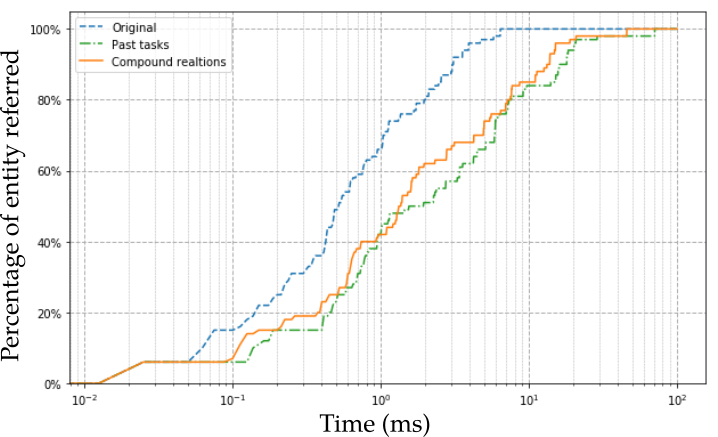
\includegraphics[scale=0.5]{figures/chapter7/comparison.png}
\caption{\label{fig:chap7_compare} Comparison of the three algorithms regarding the percentage of successfully referred entities over time using a logarithmic timescale. }
\end{figure}

The original algorithm has been run without the possibility to use relations toward task since it is not designed for this use. Its performance is our comparison point as we expect all algorithms to find the same solutions. For the recall, the described tasks are designed in such a way to not help in the \acrshort{re} generation and but ourselves in the worst case. The measures of the percentage of entities referred over time for all three algorithms are represented in Figure~\ref{fig:chap7_compare} and reported on appendix~\ref{app:reg_comp_solutions}.

With this setup, the current version performs slightly better than the previous one with an average resolution time of 4.17ms versus 5.53ms. It is however more than the original version having an average resolution time of 1.08ms. This difference must be qualified by the exploration of \acrshort{cr}s that the original one does not do. While the majority of the entities are referred in a comparable time with the previous version, we can still note that the more complex entity requiring six relations is now solved in 45.71ms versus 70.57ms previously.

An advantage of the current algorithm is that in the case no \acrshort{cr}s are described the performance are the same as the original algorithm. At the difference, the previous version had an impact even if negligible. 

% chap 4
%count    77.000000
%mean      1.080750
%std       1.355236
%min       0.013237
%25%       0.193782
%50%       0.516371
%75%       1.322064
%max       6.405807

% chap 6
%count    77.000000
%mean      5.531283
%std       9.780631
%min       0.012952
%25%       0.509738
%50%       1.538461
%75%       5.968753
%max      70.577606

% chap 7
%count    77.000000
%mean      4.178141
%std       6.855033
%min       0.016902
%25%       0.438766
%50%       1.323878
%75%       5.447168
%max      45.716713
\ifdefined\included
\else
\setcounter{chapter}{8} %% Numéro du chapitre précédent ;)
\dominitoc
\faketableofcontents
\fi

\chapter{A robot in the mall: The MuMMER project}
\minitoc

This chapter is a sum-up of an article submitted to the  User Modeling and User-Adapted Interaction (UMUAI) Journal. This work has been achieved in collaboration with Amandine Mayima, Guilhem Buisan, Phani-Teja Singamaneni, Yoan Sallami, Kathleen Belhassein, and Jules Waldhart. In this chapter, we first give an overview of the European H2020 Project \acrfull{mummer}\footnote{\url{http://mummer-project.eu/}}, in the context of which the contribution of chapter~\ref{chap:3} was made. We then present the components developed by the LAAS-RIS team with a focus on the component in which I participated as well as their integration in a robotic architecture.

\section{Introduction}

In large scale, indoor environments, like museums, shopping malls, or airports, the presence of large interactive screens, maps, or signs underline the importance of providing information on itineraries. However, reading such maps can be challenging and some information can be missing like the location of the shops selling a given product. To bring such new information and help people to find their itinerary in large indoor environments such as shopping malls, robots can be used.

To study this challenge and the underlined Human-Robot Interaction requirement, in the context of the European H2020 Project \acrshort{mummer}~\cite{foster_2016_mummer}, we have developed and deployed a social service robot in one of the largest malls of Finland, Ideapark in the city of Lemp\"a\"al\"a. The resulting robot is able to chat with customers and guide them. The chatting has been brought by a partner of the project. The contribution of the LAAS-RIS team, and thus the focus of this chapter, was on the direction-giving task.

With a mall having approximately 1.2 kilometers of pedestrian streets and more than 150 shops, having a robot accompanying customers would be time-consuming. Taking inspiration from the mall employees, we chose to verbally describe the route while grounding it with pointing gestures. The robot can however move a few meters if needed. %Such a movement can be useful to improve the perspective sharing of landmark to better ground the route description.
The output of this project is a complete robot architecture that integrates a number of components. Each of them makes use of various models and decisional algorithms, all integrating explicitly human models.

First, we provide background information about robot guides and discuss how the human partner has been considered. Then, we present the human-human exploratory studies used to identify the required abilities for a guide robot. We then present the developed architecture and its components. We end this chapter with integration on a real robotic system with some detail on its deployment "into the wild".

\section{Related work}

A number of contributions have proposed robot guides, from the first museum guides \cite{burgard_1999_museum, siegwart_2003_robox, clodic_2006_rackham} to more recent robot guides in large areas \cite{bauer_2009_autonomous, triebel_2016_spencer}. A recent example is presented in \cite{chen_2017_robots}. The developed robot is able to accompany the customer to its destination, then to point at it. Another robot presented in \cite{gross_2009_toomas} can help the customer to find specific product among all the shops of a mall. Most of these works are focused on the navigation aspect of the task. It requires environment mapping, localisation, and social navigation due to the presence of many humans.

Where previous contributions were mostly focused on navigation, others have investigated the direction-giving task, meaning the fact to not accompany the customer but to describe the route to the goal. For example, \cite{cassell_2007_trading} describes an embodied conversational agent giving route directions using deictic gestures. Within the Robovie project, the ATR-IRC laboratories have developed a robot providing route description through the use of utterances and gestures, and have highlighted the importance of their timing~\cite{okuno_2009_providing}. Kanda et al. in \cite{kanda_2009_affective} and \cite{kanda_2010_communication} have divided the direction giving into two steps. First the robot point toward the direction to take, then it explains the full route. In addition, the robot can give recommendations for restaurants and shops. Finally, \cite{satake_2015_should} showed a complete architecture of an information-providing robot able to move around a square in a mall. It embedded a map, an ontology, a speech recognition system, a dialog manager, a localization module, and a people tracker. As in their previous works, the robot verbalized utterances and used deictic gestures to give route directions. Numerous other contributions can be found but, only a few of them propose full architectures for an autonomous direction-providing robot, the most complete one being the Robovie robot presented above. 

To the best of our knowledge, no system tackles the guiding-task by reasoning about the shared perspective. If the robot has to point a landmark not visible by the human at its current position, we want the robot to pro-actively propose to the human a pertinent placement. This is one of the basic bricks of our system and it is strongly linked to the key principles of Joint Action which involve the ability to establish and monitor joint attention~\cite{pacherie_2012_phenomenology}.

\section{Learning from exploratory studies}

To lead to robot abilities design and implementation, two human-human exploratory studies were conducted in collaboration with VTT Technical Research Centre of Finland. In addition to the current literature, it allows us to enrich our knowledge with effective route descriptions in the robot deployment environment.

The first pilot study consisted of a human guide providing route information. It consisted of one participant asking for shop directions to a guide working at the mall information booth. The analysis focused on gestures used to give guidance, the positions of the two protagonists in relation to the target shop and their interlocutor, and the gazes alternation. \cite{belhassein_2017_human} gave the first indications to consider resulting from this pilot study. Among these results, we can note a preference over the ipsilateral hand to the visual field of the target. This study also provides numbers of dialogue transcription use to study how guides effectively provide route description and give examples of descriptions.

\begin{figure}[ht!]
\centering
\includegraphics[scale=0.35]{figures/chapter8/human_guide.png}
\caption{\label{fig:chap8_human_guide} Picture from the second Human-Human study \cite{belhassein_2017_human}. Here, the guide is giving the route description to reach a given shop by pointing at it. The formation formed by the guide, the customer, and the target was analyzed. }
\end{figure}

A second exploratory study was then carried out to focus on more complex situations. Among them, we can note situations with two customers requesting directions simultaneously, a customer requesting for two shops at the time, or someone interrupting an ongoing interaction. Once again the formations were analyzed. An example of such a formation seen during the study can be seen in figure~\ref{fig:chap8_human_guide}. The full results can be found in~\cite{Heikkilae_2018_where} and~\cite{heikkilae_2019_should}. Among these results, the study has shown that the guide usually points to the general location of the target first and in a second step explain and point the different stages of the route.

\section{The deliberative architecture}

In this section, we present the robotic architecture developed to handle the direction-giving task. This architecture relates to Beliefs, Desires, Intentions (BDI) architectures. As explain by~\cite{wooldridge_1999_intelligent}, such a kind of architecture is primarily focused on practical reasoning, meaning the process of deciding step by step which action to perform to reach a goal. 

\begin{figure}[ht!]
\centering
\includegraphics[width=\textwidth]{figures/chapter8/architecture.png}
\caption{\label{fig:chap8_architecture} The general architecture developed for the robot guide. The components presented in this chapter are the colored blocks. The red components with the symbol * are the ones on which I participate. The visual perception and dialogue components have been respectively developed by IDIAP and HWU and are described by~\cite{foster_2019_mummer}. Naoqi is a Softbank Robotics software. }
\end{figure}

The figure~\ref{fig:chap8_architecture} represents the architecture, its components, and their interconnections. Communication between component relies on ROS. In this chapter, we only present the components developed by the LAAS-RIS team, represented by the colored blocks on the architecture. First, we present the two knowledge representations in the form of geometric and semantic representations. Next, we introduce the components related to the sensorimotor layer. It is the situation assessment and the physical resource manager. Then, we present the components related to the deliberative layer. They are the Human-Aware Navigation, the SVP planner, the Route Handler, and finally, the one linking all the components, the Supervision. The Route Handler, part of the deliberative layer, having been presented in detail in chapter~\ref{chap:3}, will not be detail in this chapter.

\subsection{Environment representation}

For a service robot providing directions to people, we needed information to understand humans' need, information to compute the route to the goal, and information to compute the visibility of both agents to plan the pointing position. To understand the needs of a human wanted to be guided, we need information about the type of stores and the sold items. To provide so, \cite{satake_2015_field, satake_2015_should} used an ontology. To compute the route to the final destination, \cite{matsumoto_2012_you} or \cite{okuno_2009_providing} used a topological map. Wich node of the graph is related to a 2D position of the environment. To estimate the human visibility of elements anywhere in the environment, \cite{matsumoto_2012_you} used a simplified 3D model where shops are represented by 3D polygons. In our implementation, we only used two types of representation of the environment: a \textbf{geometric} and a \textbf{semantic}.

Since the final deployment of the robot is in a Finland mall, we have built an emulated mall in our lab for development purposes. The representations describe hereafter have thus been created both for the real mall and the emulated one.

\subsubsection{Geometric representation}

The geometric representation is used to compute the visibility of elements of the environment from different positions needed for the pointing of landmarks. However, because the robot does not accompany the person to the final destination and therefore does not move much, the possible visibility of the two agents is limited to their immediate environment. For this reason and due to the large scale of the Finland mall, we chose to geometrically describe only the subpart of the global environment that could be visible from the interaction area. For the rest of the environment, we represented the shops with 3D points only. These points are enough to point in the right direction. The resulting geometrical representation is a three-dimensional mesh model, as shown in figure.~\ref{fig:chap8_adream_base} for the emulated mall and in figure~\ref{fig:chap8_ideapark_base} for the real one. We have represented in the 3D model all the elements that could hinder visibility, such as poles or panels. In this way, we can precisely emulate human visibility. The model was created from the architectural plans first and then refined with measurements in the mall.

\begin{figure}[ht!]
\centering
\includegraphics[scale=0.15]{figures/chapter8/adream_base_m.png}
\caption{\label{fig:chap8_adream_base} The 3D mesh model of the emulated mall at laboratory. The red square represent the interaction area as a square of 4 meters per 4 meters. Signs representing the shops have been place all around the environment. }
\end{figure}

\begin{figure}[ht!]
\centering
\includegraphics[scale=0.15]{figures/chapter8/ideapark_base_m.png}
\caption{\label{fig:chap8_ideapark_base} The 3D mesh model of the real mall in Finland. The entire mall having a size of 528.6 meters per 247.5 meters on two levels, we have only modelled the part which can be visible from the interaction area. It results in a model of 150 meters per 69 meters. }
\end{figure}

In order for the pointing planner to compute the visibility of the landmarks used for the route description, stairs, escalators, elevators, and store signs are represented each by a single mesh while the rest of the building is a unique 3D mesh. This means that a store is said to be visible if we can see its sign, which we think to be the most relevant element to see to recognize a shop.

The 3D model is also used to generate a navigation map, constraining the robot to move in the interaction area while avoiding obstacles in it.

\subsubsection{Semantic representation}

The environment semantic representation is oriented toward communication and human navigation in a mall. It makes use of the terms, affordances and actions that are needed to walk around in the mall. It represents the needed human-robot common ground knowledge and is used by the robot to perform dialog acts concerning shop names and categories a well as the types of products sold.

This representation takes the form of an ontology. It uses the \acrfull{ssr} to describe the environment topology. The notion of place is then extended to represent information about the stores. It allows to define and refine the shared goal of the task by understanding the client's wanted destination. We thus represented in it the stores' types, their names, and the items they sell with a rich semantic. It allows for example to represent that both soda and hamburgers are sold in fast-foods, which are types of restaurants, but that soda can also be found in a supermarket. Thanks to Ontologenius, the names of concepts are defined in different languages and with synonyms for these names. It allows the robot to adapt itself to the human partner language. Moreover, with Ontologenius, we endow the robot with the ability to recognize a set of names in natural language but that it will be prevented to use. For example, the robot can understand a reference to ``bank'' when a human says it but only refers to it as ``ATM'' or ``cash machine'' since there was no bank office in the mall. In addition, we used the provided fuzzy matching service to help the supervision system to handle ambiguities coming from the speech-to-text component. For example, if the language recognition module catches the word ``Juwelsport'', we can match it with ``Juvesport'', being a shop in the mall. This set of functionalities around the concepts' names facilitates the understanding of the partner's need and thus helps at increasing the quality of interaction.

\begin{figure}[ht!]
\centering
\includegraphics[scale=0.45]{figures/chapter8/zizzi.png}
\caption{\label{fig:chap8_zizzi} Representation of the knowledge about the shop H\&M stored in the ontology. We have both purely semantic knowledge and topological information. }
\end{figure}

An example of the final semantic knowledge represented in the ontology for a given shop is presented in figure.~\ref{fig:chap8_zizzi} for a clothes shop called ``H\&M''. We find in this description the identifier of the shop, the category to which each store belongs, the topological information, the items sold and the names and synonyms in natural language and that for different languages.

\subsection{Perceiving the partner}

The situation assessment component is based on the Underworld framework~\cite{lemaignan_2018_underworlds}. It aims at gathering perception information in the form of 3D position and orientation of human faces, with the 3D model and the robot state. With this information, it is able to generate the symbolics facts listed in table~\ref{tab:chap8_predicates}.

\begin{table}[ht!]
    \centering
    \begin{tabularx}{\textwidth}{|l|X|}
     \hline
    \textbf{Predicate} & \textbf{Description} \\
    \hline
    \hline
        isPerceiving & The robot is perceiving a human \\
        \hline
        isCloseTo & The human is within a distance of 0 to 1 meter of the robot \\
         \hline
        isLookingAt & The human is looking at the robot \\
        \hline
    \hline
        isInArea & The human is in the interaction area \\
        \hline
        isEngagingWith & The human is close to the robot and is looking at it \\
       \hline
    \end{tabularx}
    \caption{Facts computed and monitored during the direction-giving task.}
    \label{tab:chap8_predicates}
\end{table}

\subsection{Managing the robot's resources}

A humanoid robot such as Pepper can be seen as a composition of multiple physical components that can act independently of each other. For the pointing task, we identified four resources: the head, both arms, and the base. At the beginning of the interaction, for example, the head is used to find people to interact with, but later it will be used to track the human with the gaze. Several components could access this resource to perform these actions. However, they do not have a global picture of the ongoing task. In this case, a resource could be used by several components at the time. Consequently, it could lead to task failures.

Moreover, in some cases, several resources have to be used simultaneously to perform a high-level action. To point to a landmark, one arm is selected to point while the other has to be lowered. The base is then rotated if the arm reaches the joint limit to point a target on its back. If at least one of the involved resources is simultaneously used to perform another action, the overall high-level action will fail as the global posture will no more be clear. For example, if the human gets too close to the robot and a component tries to move even a bit to move away from a little, the arm would no more point in the right direction.

Thus, the correct handling of all the resources is critical for performing the task, but it can be cumbersome for a deliberative component, such as the Supervision, to do all the micro-management required. To tackle this issue, we designed a physical resource management system to provide an abstraction of each resource. For each of the identified resources, we instantiated a component called \textbf{Resource Manager (RM)}, having multiple inputs. It is endowed with a low-level decision-making ability allowing it to vote for the next command from a given input to be executed. Its choice is based on events, priorities, and commands importance. Inputs are divided into two types: \textbf{atemporal inputs} and \textbf{finite state machine inputs}. Atemporal inputs are unit overwriting buffers receiving commands which can be run continuously and preempted at any time. Each atemporal input has semantic meaning. For example, the head manager has an atemporal input dedicated to the monitoring of the interacting human. This input thus receives permanently a command to look at the head of the human to be monitored, even if we do not have to look at him. When this input is voted, the robot looks at this point. Finite state machine inputs are prioritized queues of state machines. Each state corresponds to a command to be executed. Transitions can be events received from other components or durations. In this scheme, a state machine cannot be preempted, as it is seen as a set of commands being part of the same high-level action, like a pointing.

To deal with high-level actions requiring multiple resources, we created a \textbf{Resource Synchronizer}. It does not have atemporal inputs but only one finite state machine inputs. It can thus receive finite state machines handling multiple resources, so-called coordination signals. The synchronizer checks if the needed resource managers are free or preemptable, if so, it dispatches the state machines to the proper resource managers and ensures their synchronicity when needed. The synchronizer also reports the status of the ongoing coordination signal to the Supervision component to monitor the progress of the action.
The global resource management scheme is illustrated in figure~\ref{fig:chap8_rm} with four resource managers and one synchronizer.

\begin{figure}[!hb]
\centering
\includegraphics[scale=0.33]{figures/chapter8/rm.png}
\caption{\label{fig:chap8_rm} Representation of the resource management system with four resource managers and a synchronizer. The red arrows represent the state machines inputs and the blue arrows represent the atemporal inputs.}
\end{figure}

\subsection{Describing the route to follow}

The route description process has already be presented in chapter~\ref{chap:3}. However, in the context of the \acrshort{mummer} project, the robot has to be deployed in a Finnish mall. Consequently, the description of the route to follow has to be in Finnish.

The Finnish language is not suitable for pattern-based solutions with placeholders to fill. Indeed, the nouns and verbs have a large number of inflection types, some of which are more common than others. Since it would be too difficult to build sentences as we did for the English version, we chose to generate the explanation in English and then translate it using the Google Translate API. An issue with this solution is that even the names of the stores are translated by giving incorrect sentences. We could think to fill the placeholders after the translation but in some types of sentences, store names would have to be declined. To pass over this later issue, we have limited the variety of sentences to only keep the ones for which it is not necessary to decline store names. This gives less diversity in the way the robot expresses itself but allows reliable translations. Finally, in some cases, we had to degrade the English quality, creating syntactically incorrect English sentences, so the Finnish translation can be right.

\subsection{Planning a shared visual perspective}

When the robot has to point to a target, two criteria have to be respected. First, the human has to be able to see the target. Second, the human has to be able to look at the pointed target and at the robot without turning the head too much. It goes the same for the robot as it has to see the pointed target, meaning to point toward a wall and be able to simultaneously point at the target and look at the human. Consequently, to point a target in its back, it has to move. The robot and the human can thus move in the interaction area during the direction-giving task, to move to a better position for pointing at the target. To find the robot and human possible positions we designed a component called the SVP (Shared Visual Perspective) Planner, presented in~\cite{waldhart_2019_reasoning}. For the purpose of the deployment, the presented version is an adapted and slightly simplified version.

To compute the visibility of both agents, the planner has access to the geometrical representation of the environment and the agents current positions. In addition, it considers an estimated agent's maximal speed to move and a visibility threshold.

When the robot explains the route to the human and points to a landmark, they form what is called an F-formation. Kendon explains that \textit{``An F-formation arises whenever two or more people sustain a spatial and orientational relationship in which the space between them is one to which they have equal, direct and exclusive access''} \cite{kendon_1990_conducting}.
This F-formation has been decomposed in \cite{mcneill_2005_gesture} into two types: the social formation and the instrumental formation. While the first type corresponds to the original definition, the instrumental formation includes a physical object that all the agents can gaze at. This means that once the robot will have moved, the human will come in front of it creating a social formation in the form of a vis-a-vis (each facing the other) and when the robot will point they will change for an instrumental formation. Indeed, when both agents will reach their position computed by the planner, we want them to be able to go from one formation to the other with only a rotation; the human will not need to move again from their arriving position to see what the robot will point. 

\begin{figure}[ht!]
\centering
\includegraphics[scale=0.25]{figures/chapter8/grid_map.png}
\caption{\label{fig:chap8_svp_grid} Visibility grid for a target located at the top right. The uncoloured areas represent an absence of visibility and the others represent the cost of visibility ranging from yellow for low visibility to purple for good visibility. The robot and the human in transparency on the image represent the final calculated positions while the others are the initial positions. }
\end{figure}

To search for better positions to reach in order to point a landmark, the planner takes three main parameters into account:

\begin{itemize}
    \item Visibility constraint: The two agents can see either the target shop when it is the only element of the route or the passage.
    \item Navigation distance cost: The agents do not have to move too much.
    \item F-formation cost: The human-robot-target angle and a robot-human-target have to be less than 90${^\circ}$. 
\end{itemize}

To compute the positions, the interaction area is firstly decomposed into a weighted three-dimensional (x,y for the possible positions in the area and z for the human height) grid representing the estimated human visibility of the target. The target visibility is computed offline for each position of the grid. It is based on the share of the target in the 360${^\circ}$ field of view of the environment. Such grid is represented in figure~\ref{fig:chap8_svp_grid} for a given human height. The white cells are positions from which the human cannot see the pointed target. The other colored cells represent the degree of visibility from the poor in yellow to the good in purple. Having the human visibility grid, the goal position is computed using a weighted cost function between good visibility and restricted distance to cross. In the example figure, the transparent human head is the human goal position while the other is the initial position. From the initial position, the human was not able to the pointed target.

The overall computation flow is illustrated in figure~\ref{fig:chap8_svp}. The robot position is computed in a second time, according to the human planned position. Divided the search into two steps allows reducing the search complexity. The robot position is thus constrained by the human one. It has also to respect a minimal and maximal distance to the human and minimal visibility of the target from it. Finally, the robot position is also determined regarding a cost preferring an F-formation limiting the robot reorientation, meaning that it can point to the target keeping its torso its chest oriented towards the human.

\begin{figure}[ht!]
\centering
\includegraphics[scale=0.45]{figures/chapter8/svp.png}
\caption{\label{fig:chap8_svp} Human and robot positions computation flow. The purple blocks represent the initial positions while the blue ones represent the planned positions. }
\end{figure}

\subsection{Navigate close to human}

The Human-Aware Navigation component aims at moving the robot while avoiding dynamic and static obstacles in addition to proposing a socially acceptable navigation solution for the robot. For example, the robot should not pass too close to the human and should not show its back while navigating around the human. A full presentation of the planner is available in~\cite{singamaneni_2020_hateb}.

\subsection{Executing and controling the task}

%Finally, there is the deliberative layer. A component, the Supervisor, implements joint action guidelines in order to manage the direction-giving task as a human-robot joint activity. It makes use of a number of human-aware decisional modules: establishment of shared goal through dialogue, planning taking into account human preferences, planning for both in order to ensure a pertinent placement of the human and the robot, reasoning and adapting to human perspective of the scene, monitoring human commitment and step by step contribution to the joint task. The action sequencing and the incremental task-refinement process follows the steps and the main decisions exhibited in the human-human studies. Not only the Supervisor takes the human into account but the other components of our deliberative layer as well, enabling the robot to be human-aware at each step of the collaborative task. The \textit{Route Handler}, based on the \textit{Semantic Representation}, deals with the entire description of the route, from the search for the best route to get to humans to their final destination, to the verbalization of this route which takes into account human orientations. The \textit{Human-aware Navigation} of the robot is implemented using a reactive navigation planner. This algorithm is able to plan and continuously adapt robot motion close to humans while respecting social constraints. The \textit{Shared Visual Perspective (SVP) Planner} helps to overcome the possible blocking of the visibility of important landmarks while giving directions, trying to find a position where the human will have to be in order to observe the route passage and also to find one for the robot which satisfies a nice human-robot-landmark conformation for pointing. Finally, The \textit{Dialogue} has been developed by HWU and is described by~\cite{Papaioannou2018}. We will not further go in the details about the functioning of this component as it is out of the paper scope. 

\section{Embody architecture in a physical robot}

\subsection{Pepper in Ideapark}

\begin{figure}[ht!]
\centering
\includegraphics[scale=0.15]{figures/chapter8/pepper_mall.png}
\caption{\label{fig:chap8_pepper_mall} todo. }
\end{figure}

\subsection{Pepper "in the wild"}
\ifdefined\included
\else
\setcounter{chapter}{8} %% Numéro du chapitre précédent ;)
\dominitoc
\faketableofcontents
\fi

\chapter{The director task: Assessing cognitive architectures}
\chaptermark{The director task}
\minitoc

The contribution presented in this chapter is excerpted from our work, submitted to the RO-MAN 2021 conference. This contribution closes this thesis and has been achieved in collaboration with other PhD students of the HRI teams. Guilhem Buisan was concerned about the task planning part. Amandine Mayima worked on the supervision component. Kathleen Belhassein has designed the presented task with us giving her psychologist point of view to create a task on which user studies could be performed. The engineer Yannick Riou worked on the motion planning component allowing us to develop a task where the robot acts on its environment. My concern about this task has been the integration of my previous contributions about Ontology and the REG. It has also been the opportunity to create an entire architecture extending the ones presented all along with this thesis and linked with the contributions of the team. Finally, I contribute to the Situation assessment component and on the Language understanding part.

The components related to my teammates will be briefly described to give an overview of the architecture. The newly introduced capabilities on which I work will be more detailed to explain the links I make between all my contributions, centred on the knowledge representation.

\section{Introduction}

Developing robotic architectures adapted to Human-Robot Interaction and thus able to carry out interactions in an acceptable way is still today a real challenge. The complexity comes, among other things, from the number of capabilities which the robot must be endowed with and therefore from the number of software components which must be integrated in a coherent manner. Such architectures should provide the robot with the capability to perceive its environment and its partners, to merge and interpret this perceptual information, to communicate about it, to plan tasks with its partner, to estimate the others' perspective and mental state, etc. Once developed, evaluating these architectures can be difficult because all these components grouped into a single system. The tasks we usually want the robot to handle must highlight a maximum of abilities, while still being simple enough to be reproduced by the community. Moreover, we should be able to conduct user studies with it to validate choices regarding naive users.

Since a long term goal of the robotic field is to see robots evolving in our daily life, many tasks and scenarios have been inspired by everyday activities. Even if these tasks offer a large variety of situation to ba handle since the human partner is not limited in its actions, they have the disadvantage of not highlighting some subtle abilities which are nevertheless necessary for good interaction.
The robot guide task \cite{satake_2015_should} in mall, museum, or airport, requires high communication skills to understand free queries (possibly involving chatting) and respond to them, whether to indicate a direction or to give advice. However, the perception needs can be limited due to the vast environments, as well as the perspective-taking needs due to the same perception of the environment by the robot and the human\footnote{For sure we can find some tricky cases where it could help but they do not reflect common situations.}. Finally, with such a task the human partner is not an actor of the task and just has to listen to the robot once their question is asked. Even if being in more constrained environments, bartender-like tasks~\cite{petrick_2012_social} have the same disadvantages. Indeed, the human is considered as a customer, and as such, the interaction with the robot is limited. The robot will never ask the human to help it for performing a task and their actions do not require coordination either full collaboration.

To involve the human partner in the task and requiring him to act with the robot, assembly-like tasks~\cite{tellex_2014_asking} can be used. Nevertheless, in most cases, the human acts as an assistant rather than as a partner as full collaboration can be challenging to perform. The robot thus elaborates a plan and performs the assemble, then asks for help when detecting errors during the execution (e.g., when it cannot reach some pieces). Here the task leads to unidirectional communication. Moreover, because in such a task both the robot and the human have equivalent knowledge about the environment, it can be hard to design situations where belief divergence appear and thus perspective-taking would be required.

Scaling down an everyday task to transform it into a toy task around a table can deduce the task complexity and allow easy reproducibility. Moreover, it allows making the robot and the human work in the vicinity of each other, with smaller robots for example. With the toy version of the assembly task presented in~\cite{brawer_2018_situated}, the human is more involved in the task. They ask the robot to take pieces and to hold them to help them assemble a chair. Even if the communication is unidirectional, we could imagine inverting the roles to test different abilities. Moreover, communication implies objects referring with the use of various visual features about the entities. Even if both agents have the same knowledge about the environment, the communication is grounded according to the current state of the world. In this task, no decision has to be made by the robot but once again, inverting the roles could open other challenges.

To focus studies around perspective-taking and belief management, the Sally and Anne scenario, coming from a psychology test, has been studied in robotic~\cite{milliez_2014_framework}. In this scenario, the robot is a spectator of a situation where two humans come and go from a room, and move an object from a box to another. Since a human is in the room when the other is acting, a belief divergence appears between the two humans and the robot has to understand it. While the task highlights the belief management, it is first limited regarding the perspective-taking since the human presence or not could be sufficient to estimate the humans beliefs\footnote{When both humans are in the room they have the same perception of the scene but have different beliefs about hidden objects. Perspective-taking would be required if the humans could lean over the boxes to check what is inside.}. Moreover, the humans do not act with the robot since it is just a spectator of the scene. In addition, no goal is formulated and the human neither interacts with one another. Finally, no communication is needed in the task. The scenario is thus focussed on the analyse of a situation.

In this chapter, we first propose a new psychology-inspired task that we think to be challenging for the Human-Robot Interaction community and rich enough to be extended: the Director Task. Inter alia, it requires perspective-taking, planning, knowledge representation with theory of mind, manipulation, communication, and decision-making. Then, we present the robotic cognitive architecture that we develop to perform the task in its nominal cases. Finally, on the basis of the presented task and what has been developed, we present a discussion about the possible future challenges and evaluations for the research community, with possible extensions of the task.

\section[From psychology to Human-Robot Interaction]{The Director Task: From psychology to Human-Robot Interaction}

In this section, we present the origins of the Director Task and the needs it aims to respond to regarding other tasks from the psychology. We then detail the setup we have designed in terms of objects characteristics and organisation in the environment. We end this section with our adaptation and the required abilities we have identified.

\subsection{The original task}

The Director Task has been mainly used in psychology researches as a test of the Theory-of-Mind usage in referential communication. This task originates from a referential communication game from~\cite{krauss_1977_social}. In this game, two participants are one in front of the other with an opaque panel between them. A speaker as to describe odd designs to a listener, either to number them for the adults or create a stack of cubes for the children. To refer to the odd figures, participants have to use images (e.g. "it looks like a plane").

This game was then adapted by Keysar et al.~\cite{keysar_2000_taking} and become the Director Task. It has been used to study the influence of mutual knowledge in language comprehension. In this task, two people are placed one in front of the other but instead of an opaque panel between them, they place a vertical grid composed of different cells and objects in some cells. The \textbf{director}, a participant or in most cases an accomplice, instructs the \textbf{receiver}, a participant, about objects to move in the grid. The receiver thus follows the director's instructions about objects to move. The particularity of the task is that some cells are hidden from the director meaning that the receiver, being on the other side of this grid, does not have the same perspective as the director. He thus knows the content of more cell than the director and consequently sees more objects. When the director instructs the receiver to move an object, for a successful performance, participants must take the perspective of the director to move the right one. Because the configuration evolves all along with the task, he has to update this estimated perspective all along with the interaction.

\begin{figure}[ht!]
\centering
\includegraphics[scale=0.25]{figures/chapter9/dt_apple.png}
\caption{\label{fig:chap9_dt_apple} Sample display from the director's and the receiver's perspectives. The asterisk indicates the target object. Giving the sentence "the smallest apple" the receiver should find the good one even if he can see a smallest one in its perspective. }
\end{figure}

Taking the example of figure~\ref{fig:chap9_dt_apple}, if the director instructs the receiver to take the smallest apple, the target object in its perspective is the one marker with the symbol *. However, for receiver, in its perspective, the target object is not the smallest apple since the smallest one (called distractor) is only visible by the participant and not by the director. The participant then must understand the director's perspective to take the target apple and not the distractor. Some studies showed that for their first attempt, participants took the smallest apple from their own point of view and only after, the target one. These results were interpreted in~\cite{keysar_1994_illusory, keysar_1998_egocentric, keysar_2002_self, keysar_2003_limits} as the participants understanding language in an egocentric way. Some social cognition studies used a computer-version of the Director Task~\cite{dumontheil_2010_online} whose results are consistent with the ones mentioned previously, namely that participants do not use Theory-of-Mind inferences in language interpretation.

Although Theory-of-Mind and perspective-taking both require the attribution of mental states to others, some authors trend at distinguising Theory-of-Mind tasks and perspective-taking tasks as involving distinct although related mechanisms. In~\cite{santiesteban_2012_training}, they considered in their study that perspective-taking abilities were measured by the Director Task whereas Theory-of-Mind usage was investigated through another task called ``strange stories''~\cite{happe_1994_advanced}. This Theory-of-Mind task requires the attribution of mental states to a story protagonist, meaning to maintain an estimation of others' mental states. At the difference, the Director Task requires for adopting the perspective of the director in order to follow their instructions, meaning to use this knowledge in order to execute the task properly. 
In this way, the authors estimated that the Director Task requires a higher degree of self-other distinction by continuously isolating our own perspective from the director one, in order to use them to act. In addition to perspective-taking abilities, the Director Task makes use of executive functions~\cite{rubio_2017_director} (i.e. vary the processing of information according to current goals in an adaptive manner) and attentional resources~\cite{lin_2010_reflexively}.

To summaryse,the Director Task has been used to study referential communication, language comprehension, and perspective-taking abilities. However, to our knowledge, it has never been exploited in the context of a HRI although this task presents interesting challenges for this field. More than technical challenges, it provides a way to investigate the different cognitive and behavioral processes involved in such a cooperative Human-Robot task.

\subsection{The Director Task setup}

The material used in this task has been chosen to be easily acquired and can be hand-built. It is composed of blocks, compartments, and a storage area. Each element is equipped with AR-tags allowing the robot to perceive them without advanced perception algorithms.

\begin{figure}[ht!]
\centering
\includegraphics[width=\textwidth]{figures/chapter9/material.png}
\caption{\label{fig:chap9_material} Part of the material used for the Director Task. Each element is equipped with AR-tags allowing their detection by the robot. Each block has four visual characteristics: a main color, a border color, a geometric figure  and a figure color. }
\end{figure}

Three types of compartment exist and are illustrated on the right part of figure~\ref{fig:chap9_material}. The basic ones are open on two of their opposite sides (d). They allow both the receiver and director to see the content and to manipulate it. Others are open only on one of their sides (e). With such a compartment, only one of the participants can see and take what is inside. The other participant can neither know if a block is inside or not. The last compartment type (not used in the implemented version) has an open side and the opposite one equipped with a wire mesh (c). Because of the side with the wire mesh, both participants can see what is inside but only one of them can take it. Thanks to these three types, we will be able to vary the awareness of the blocks (e.g., a block is known to be present but not necessarily visible), the visibility of the blocks, and their reachability (e.g., a block can be visible but not reachable). While the original Director Task uses a vertical grid, we prefer here to use several compartments to create the grid. It allows more modularity to create different situations.

Where the tasks used in psychology use everyday objects, we rather choose blocks that can easily be manipulated by robots and on which we can fix tags for their detection (a-b on \ref{fig:chap9_material}). The blocks have a primary color covering them all. On two opposite faces, additional visual features are drawn. The top part of these faces is dedicated to the robot's perception with a unique AR-tag on each face\footnote{Since the tags are different on each side, the director can not refer to them as the receiver does not see the same ones}. The bottom part is the same on both faces and is dedicated to human perception. In addition to the primary color, three visual features are available by the human to distinguish them being: a colored border, a colored geometric figure (both the color and the figure can change making two features). Every visual feature (the colors and the forms) has exactly two variants. The colors are either blue or green and the figures are either a triangle or a circle. We can thus have 16 unique blocks.

The agents can use the four visual features to refer to a specific block and the complexity of the description depends on the used features. While the main color is directly related to a block, the other colors are respectively related to the border and the figure. In this way, for two blocks whose only difference is the color of one of these elements, the said element has to be referred to in order to refer to the divergent color. A description of a block involving all its four features would be ``the [color] block with the [color] border and the [color] [figure]''.

The figures and colors have been chosen in such a way to allow the emergence of ``coded words'' between the participant to identify a block. With a bit of imagination, some could refer to the left-most block (a) through the sentence ``the mountain in the sea'' or the other (b) by ``the puddle''.

\begin{figure}[ht!]
\centering
\includegraphics[scale=0.15]{figures/chapter9/positions.png}
\caption{\label{fig:chap9_positions} The Director Task setup with the robot and the human partner one in front of the other and a piece of furniture between them. Compartments are placed on top of the furniture and blocks are placed in the compartments. Next to the agent having the receiver role, here the human, a storage area is placed to drop the removed blocks. }
\end{figure}

Regarding the disposition, the compartments are stack on a piece of furniture to create a kind of grid. The blocks can be put in a compartment. As illustrated in figure~\ref{fig:chap9_positions}, the two agents are placed one in front of the other with the furniture and thus the compartment between them. Finally, one storage area, corresponding to the place where the receiver has to store the blocks, is delimited by a rectangle on a shelf next to the receiver. In the figure, the human would be the receiver as having the storage area on his right.

\subsection{The adapted task}

Now we see the Director Task setup and the available material, we present the rules we have adapted for HRI applications. First, the high-level goal of the task is known by both agents: to put a set of blocks away. The precise goal is given by the experimenter to the director, either the robot or the human. It corresponds to a subset of the blocks presents in the compartment that the receiver should remove from and put in the storage area. This choice to remove the objects instead of moving them in the grid engender an evolution of the situation over time. It thus requires a constant adaptation during the interaction. The goal can be given on a sheet of paper, a screen behind the receiver, or marks on the blocks on the director side. No block order is required in the formulation of the goal. The director is thus allowed to elaborate a strategy if needed.

As mentioned previously, the Director Task characteristics bring a number of interesting challenges for a collaborative robot to solve. Because this is a task with roles, one of the first challenges is to build a robotic architecture that gives the robot the ability to play both roles. Then, each role brings some specific problems to solve from a robotic point of view.

In order to enrich the task with perspective-taking issues, we adapted the task so that both the director and the receiver have to use perspective-taking. Since in the original task, the director knows he has a subset of the receiver's perspective, he can consider all the objects when communicating. Thus, only the receiver has to reason about the other's perspective, taking into account that some objects are not visible by the director. For HRI applications, we used the one side hidden compartments in a way to also have objects hidden from the receiver and visible by the director. Therefore, both roles have to perform perspective-taking, whether to give instructions or to understand them. On the illustration of figure~\ref{fig:chap9_setup}, the director (left image) can instruct the receiver to take the blue blocks as the other blue blocks in his perspective is hidden from the receiver. From the receiver point of view (right image), he can find the said block as the other blue block is hidden from the director.

\begin{figure}[ht!]
\centering
\includegraphics[width=\textwidth]{figures/chapter9/setup.png}
\caption{\label{fig:chap9_setup} A director task setup adapted to the HRI with the director's and receiver's perspectives. For the material, each element (blocks and compartment) is equipped with AR-tags allowing their detection by the robot. Each block has four visual characteristics: a main color, a border color, a geometric figure, and a figure color. Compartments can be hidden for the director or the receiver. For the director to designate the block marked with a red circle, estimating the receiver's perspective, he can refer to it by its main color (blue) because he estimates the other blue block is not visible by the receiver. For the receiver, by taking into account the director's perspective, he can understand the referred block as he estimates the other blue block to not be visible by the director.}
\end{figure}

To be able to study precise skills, such as verbal communication, perspective-taking, and adaptation, we defined a set of rules for both roles. First, the agents are not allowed to point to objects, either with their hand or gaze. They thus have to verbally describe the objects, focusing the task on verbal communication. However, to avoid too easy description of the kind ``the fully green block'', we remove the four uni-color variants\footnote{When we said too easy it is from the human point of view, generating and understanding such description can be challenging for a robot.}. In addition, to neither fall into simple referential communication task, participants are not allowed to use geometrical relations in the verbal communications. They cannot, for example, say ``the leftmost block'' or ``the block to the right of the green one''. In this way, they are limited to few visual features, with high ambiguity. Since a description of a block using its four visuals features can be hard for the human to process, we first expect the participants to minimize the complexity of their communication by referring to the blocks only using the features distinguishing them from other blocks. Moreover, we also expect the participant to take into account the other perspective allowing once again to minimize the complexity of the communication.

Over these elements, we can see that the task can easily be replicated and offer a controlled setup, making it a good task for human-robot user studies. Moreover, due to the number of involved processes and the number of situation that can be made, there are a lot of elements that can be analyzed and explored. Also, with the same setup, it is possible to perform human-human studies or human-robot studies which can be interesting to compare.

\subsection{Additional abilities}

More than being an easily reproducible scenario to perform user studies on human-robot interactions in a controlled environment, the Director Task allows demonstrating abilities of a robotic system. We detail here some additional abilities than the one the task has been designed for.

\paragraph{Planning} When a large number of blocks has to be taken in the task goal, it quickly becomes complicated to communicate about some of them as the director would have to add a lot of adjectives to be able to refer to one block. Therefore when the robot is the director, it becomes interesting to integrate the communication and the task planning. Indeed, depending on the order in which the blocks are designated, the complexity of instructions can decrease or increase. Then, the planner can return an optimal order in which the robot has to give the instructions to the human.

\paragraph{Contingencies handling} While performing the Director Task, errors can easily happen. Either because the director gives a wrong instruction or the receiver misunderstands the instruction and takes the wrong block. In both cases, it can be because of a wrong consideration of the other agent's perspective or simply inattention. Moreover, because some instructions might be right but hard to interpret by the receiver leading also to an error from them. Finally, errors can happen because of failure for the robotic system, as a failed action execution leading to a block to falls on the floor. A robot with a robust decision-making system will be able to analyze, try to determine their origin, and handle a number of these contingencies. For example, if the human takes the wrong block, the robot can react in different ways, either by asking the human to put it back if this block is not part of the goal, or saying nothing and re-planning if this block was among the ones to take. If errors happen repeatedly, the robot can also react differently than for a punctual error and maybe try to modify its behavior.

\paragraph{Communication} We saw that the task requires to put a focus on communications. The communication about an object can be more or less efficient, depending on the number of characteristics given about the object or the pertinence of these characteristics. Instructing for the blue block with a circle in figure~\ref{fig:chap9_setup}, the geometrical figure information is not mandatory. Thus, the robot needs to be able to give proper instructions but also to understand the human ones. Moreover, in complementarity with the error management, the robot can communicate to help to solve the detected contingency. Taking a situation (with the disposition of figure~\ref{fig:chap9_setup}) where the human as director instructs the robot with the green block with a circle. This instruction matching two blocks, the robot could say that it does not find the instructed block\footnote{It would be an easy solution for a stupid robot.}. A preferable reaction would be to help the human to refine the instruction and say "the one with a blue circle or a green circle ?".

\section[Architecture and knowledge link]{The cognitive architecture and the knowledge link}

In this section, we present the architecture developed to handle the Director Task in its nominal case for both roles. The architecture aims at being extending and already endow the robot with the abilities listed previously even if there are not mandatory to achieve the task. This architecture is the continuity of the one presented all along this thesis. It can also be see as a whole new instantiation of the deliberative architecture for Human-Robot Interaction presented in \cite{lemaignan_2017_artificial}. The seven identified modules are represented in figure~\ref{fig:chap9_architecture} with their respective communication links. In the rest of the section, we detail each module and how we have refined them in terms of functionality and linking. The modules already presented in this thesis will be briefly recall but not detailled in depth.

\begin{figure}[ht!]
\centering
\includegraphics[width=\textwidth]{figures/chapter9/architecture.png}
\caption{\label{fig:chap9_architecture} An overview of the cognitive architecture developed to handle the Director Task. Each block does not necessarily represent one software component but rather an architectural module (in terms of the features it implements). The arrows represent the type of information exchanged between the modules. This architecture extends the ones presented all along with this thesis.}
\end{figure}

\subsection{Storing and reasoning on symbolic statements}

The knowledge representation is always a core component of cognitive architectures as organising knowledge allows the robot to better understand the environment it evolves in. Moreover, it is on the based of these knowledge that a robot can communicate with its human partner about the current state of the world and ground the partner's utterance regarding this world state.

Some architecture propagate knowledge all along their components~\cite{hawes_2007_balt}, each of them enriching knowledge at each stage before filling it to the nexts. Others have preferred to see their knowledge base as an active server, activating perception process when needed, depending the searched information~\cite{beetz_2018_know}. For our architecture, we staied on the principle of a central, server-based knowledge base. It is refined into two distinct sub-modules, the semantic knowledge base and the episodic one. The semantic part is in charge of representing the environment elements meaning, the objects' and agents' types, their applicable properties, the descriptions and parameters of the actions, a part of the language model with verbs or pronouns, and their names in natural language. Besides, we also use it to represent the current symbolic world-state (the computed facts) and thus the instantiation of the concepts in terms of physical (e.g., this particular block) or abstract (e.g., this particular action instance) entities. Among these instantiations, we have a part used for the interaction in itself, like the blocks' visual features, and others for the robot programming, like the objects' computer-aided design (CAD) models or tags ids. The episodic knowledge base aims at keeping a trace of the symbolic transitions of the world in the time. It is strongly linked to the semantic knowledge base as it allows to semantically interpret these transitions. 

The semantic knowledge base is still an ontology managed by the software Ontologenius. The episodic one is in the form of a timeline, managed by the software Mementar\footnote{\url{https://github.com/sarthou/mementar}}.

\subsection{Assessing the world: from geometry to symbolism}

The role of the geometrical Situation Assessment module is first to gather different perceptual information and build an internal geometric representation of the world, composed of objects and agents. From this world representation, the module runs reasoning processes to interpret it in terms of symbolic statements between the objects themselves and between the involved agents and the objects. Doing so, the module only builds the robot's representation. However, it does not necessarily reflect what the human partner believes about the world. This is the case with the occluded compartments of the task. If a block is present in a compartment occluded from the human perspective, this block is not visible and thus unknown to the human. Consequently. it should not exist in the human representation of the world. Here is the second role of the Situation Assessment module, estimating the human's perspective and building an estimation of their world representation. It is the first step allowing to implement the theory of mind principles \cite{baron_1985_does}.

To implement this module, we have chosen the Underworld framework~\cite{lemaignan_2018_underworlds}. Its advantage is to not be monolithic\footnote{It can however be a disadvantage in terms of performance but for research purpose, it allows more flexibility.}. It works on the principle of a set of worlds, each working at a different granularity and providing specific features, links to create a so-called cascading structure. In the idea, it can be compared to a perception pipeline like~\cite{beetz_2015_robosherlock}. It allows easy reuse of existing modules and makes the core reasoning capabilities independent of the used perception modalities. Where we choose to use tags for objects detection, we could easily pass to machine learning approaches. In the same way, we could use it with simulations or Virtual Reality systems.

The four worlds we create for the Director Task and their connexion are represented in figure~\ref{fig:chap9_uwds}. At the top (a), we have the perception modalities. For the objects we use AR-tags~\cite{fiala_2005_artag}. For humans, we use a motion capture (mocap) system with helmets equipped with reflectors. For now, only the head is tracked. From each perception input, we create a dedicated world. In these worlds, we can filter the perception data depending on the used system. For the mocap, the data is clean enough. For the AR-tags we apply first a motion filter to discard data acquired when the robot moves. In addition, we apply a field of view (FOV) filter to discard data from the border of the camera because of distortions giving wrong positions even with camera calibration. To know to which object correspond a given tag unique identifiers (UID), the worlds have access to the ontology and can query it to get the UID related to. In the same principle, they can get the objects CAD model. As the output of these worlds, we ensure to have stable data with UID related to the knowledge base.

\begin{figure}[ht!]
\centering
\includegraphics[width=\textwidth]{figures/chapter9/uwds/uwds.png}
\caption{\label{fig:chap9_uwds} The world cascading structure of the geometrical situation assessment system. The two worlds at the top (a) are build from the perception systems and filtered. The world of the middle (b) merges the different perception information and computes symbolic facts on it. The world at the bottom (c) is the estimation of the human world representation and is computed from perspective-taking in the robot's world. Like for the world of the middle, symbolic facts are computed and sent to the semantic knowledge base.}
\end{figure}


The world of the middle (b) is the robot's world representation. Information from the perception worlds is merged along with the static elements, like the building walls, and the robot model. From this world, additional perception reasoning processes are applied for the objects that are no more visible in the way of~\cite{milliez_2014_framework}. If an entity is no more perceived in one of the previous worlds, we first test if it should be in the robot's FOV. If so, the robot should see it. To get an explanation of this absence, we test if another entity could hide it. If not, the object is removed from the world representation. Otherwise, we keep it as we have found an explanation.
Once the entities stabilised, geometric reasoners are applied to them to extract symbolic facts. In the current version of the system, the computed facts are \textit{isOnTopOf}, for an object on top of another with a direct contact, \textit{isInside}, for a block in a compartment, \textit{isVisibleBy}, assessing if an agent could see the object or not from his position, and \textit{isReachableBy}, assessing if an object can be taken by an agent. All these facts are sent to the robot's semantic knowledge base, where reasoners will deduce further facts. For example, if a block is in a compartment, thanks to inverse property \textit{hasInside} the fact that the compartment has the block inside is computed. In the same way, if this compartment is on top of the table, the block inside is computed to be above the table (\textit{isAbove)} thanks to chain axiom.

While the previous world corresponds to the robot's representation, the human partner can have the same because of the occluded compartments. The world below (c) thus aims at estimating the representation of the world from the partner's perspective. From the robot's world, we compute a segmentation image from the human point of view and use it as a filtered perception world. This allows us to instantiate the same world management process we used for the robot but this time for the human. In this way, we emulate their perception capability and geometric reasoning process. Symbolic facts are thus computed and sent to the human's semantic knowledge base. In the world of the bottom on figure~\ref{fig:chap9_uwds}, we can see that the two blocks in the occluded compartments are not present in the human world. Here we make explicit the difference between an object that is unknown and an object that is known but not visible. We could have an interaction where the human goes to see the robot side and the robot would consequently estimate the blocks in the occluded compartments as known to the human but not visible.

\subsection{Planning with symbolic facts}

The symbolic planners are divided into two categories: the domain-independent, planning high-level tasks, and the domain-dependant, specialized in solving precise problems. For the Director Task, the only domain-specific planner used is the Referring Expression Generator presented all along with this thesis. More precisely, we integrate the algorithm presented in chapter~\ref{chap:chap7}.

Where we previously used HATP~\cite{lallement_2014_hatp} as task planner, for this task we used its next-generation presented in~\cite{buisan_2021_human}. In the same way, it aims at taking into account the human's contribution to planning how to perform a high-level task. To do so, it can generate a shared plan in which parts of the task are assigned to the human partner, depending on some criteria. However, the robot's partner is not an agent that the planner can directly control. Indeed, it must sometimes communicate about the plan to inform the human about their next actions. The new planner rather trends at emulating the human decision, action, and reaction processes to generate a shared plan. For the Director Task, emulating the human reaction to a given instruction enables the comparison between multiple blocks order, the communication of higher-level instructions to the human and the balance between multiple communication modalities.

The REG planner has been successfully integrated with the new planner allowing it to estimate the cost and the feasibility of referring communication at task planning. The initial world state is fetched from the ontology leading to a uniformity of the knowledge among the architecture.

\subsection{Managing the interaction}

The supervision component aims at managing the overall interaction. In this architecture, we use JAHRVIS (Joint Action-based Human-aware supeRVISor) which constitutes the decisional kernel of this cognitive architecture. Like its predecessors, SHARY~\cite{clodic_2009_shary} and its extensions~\cite{fiore_2016_planning, devin_2016_implemented}, it is designed for a human-aware robot. It has to not only handle the robot's action execution but also estimating the human mental state, monitoring his actions, and communicate with him. To handle these features, several processes are needed:

\paragraph{Interaction sessions management:} It manage an interaction session that is first refined into tasks, themselves refine into action with the use of the task planner. Moreover, it is in charge of the greetings happening at the beginning of an interaction, the goodbyes at the end, and all events and exchanges happening outside tasks (e.g., conversation, goal negotiation) or during a task but not related to it like a human doing a parallel task on its own.

\paragraph{Communication management:} Communications are categorized in JAHRVIS either to: give information updating the receiver beliefs; ask a question to update the emitter belief; ask the other agent to perform an action; discuss with dialogue not related to a task or a goal/plan negotiation. 

\paragraph{Human management:} As the supervision manage shared plans, it has to make sure the human follows them. Moreover, even if some communications are plans, it also has to make sure that the human has all the knowledge they need for what they have to perform and if not, it hence acts or communicates through the other processes. To do so, it monitors the human beliefs about the ongoing task and plan.

\paragraph{Task management} Even if the human has also the necessary information about the plan, contingency can happen. The supervision can react and perform a repair thanks to action or communication.

\paragraph{Quality of Interaction management} Even if a task is achieved, it could be done more or less efficiently and smoothly. All along an interaction session and a task, the supervision thus estimates in real-time the Quality of Interaction (QoI)~\cite{mayima_2020_toward}. It measures the human engagement and the effectiveness of collaborative task performance. This information can then be used by the decision-making process to tune dynamically others processes such as the cost of properties for the REG.

\subsection{Speaking and understanding}

The Natural Language Generation is made of two parts, a static for actions verbs and communications to signify a lack of understanding and a dynamic part for the referring expressions. In the same way, we already done, the content is determined by the REG and the linguistic realisation is done on the basis of concepts' labels in the ontology and a simple grammar model to know in which order the adjectives have to be depending on the language.

Natural Language Understanding is more difficult due to the variety of way the same information can be communicated. Moreover, in the same communication, we have different information. In the Director Task, we have the action to perform and the object on which the action has to be performed. First, we use the Google Speech To Text (STT) API to pass from an audio stream to a string of characters. Even if such technology is now well mastered, mistakes still appear in the transcription\footnote{And this, even more, depending on our English accent and the quality of the microphone used}. On the string, we perform a first analysis trying to match words and group of words with labels of the ontology. We used sliding windows limited on the length and the fuzzy match technique available with ontologenius. To cover a maximum of possibility, several actions verbs are described as well as synonyms for the concepts. We also tried to have a good hierarchy in the ontology types for the robot to better catch the concepts depending on the abstraction level used by the human. To refer to the blocks, some only use the terms "object" as they are the only ones involved in the task. At the end of this analysis, we have a list of concepts. Depending on the number of uncaught words, we can already know if the comprehension is poor or not. On the concept list, we first extract the action verb to know the instructed action (e.g. take, place, remove). The rest of the sentence is analysed thanks to the inverse grammar model for one part but also thanks to the properties ranges and domains. When we said "the red apple", we do not have any word representing the used property\footnote{It is often the case of the attributes where relations between entities are more explicit.}. With the analyse of the usable properties linking color to an apple (and thus to a vegetable and so on), we are able to find the corresponding property. The result of this analyse is a \sparql{} query in the same way such query is used for the NLU. Depending on the number of concepts successfully linked we can estimate the comprehension quality. The \sparql{} describing the entity to act on is then merged with the context of the task and sent to the onology to find the target entity. In our case, the context would be the same as for the generation meaning that we are speaking about an object being above the table of interaction.

In the case the human gives an accurate description, we should have only one match for the target entity. However, we can not consider that the human will never do a mistake or that the robot will fully understand the instruction. In this case, we run a REG on all the ambiguous entities. The context of these generations is the \sparql{} query coming from the understanding process. If we know that we are already speaking of a green block, we do not have to recall it. We fall back into Natural Language Generation and generate sentence like "do you mean the block with a circle or a triangle ?". When the human response, we use again the \sparql{} query coming from the first utterance and merge it with the newly understood.

For the Natural Language Understanding part, we could use machine learning approaches based on sequence-to-sequence (seq2seq) models like~\cite{panchbhai_2020_exploring}. However, doing so we duplicate the knowledge already existing in the ontology to put them in a neural network. Unless creating a standard of concept identifier, such model should be trained for each used knowledge base in order to be compatible with it and use the same symbols. Having different symbols would lead to failure, having more symbols in the trained model would lead to failure (queries that could not match), and having fewer symbols in the trained model would lead to a lack of comprehension. Moreover, in addition, to create the ontology, we would have to create the corresponding training dataset that is a huge amount of work even if artificially augmented dataset creation techniques exist.

Even if our method can be seen has been ha-doc, we ensure uniformity of the knowledge among the architecture. Moreover, it can be easily extended and even dynamically extended during an interaction.

\section{Integration on a robotic system}

\subsection{The integrated features}

\subsection{Future developments}

\chapter*{Conclusion}
\addstarredchapter{Conclusion} %Sinon cela n'apparait pas dans la table des matières
Ce manuscrit de thèse rapporte 

%\ifdefined\included
%\else
%\bibliographystyle{acm}
%\bibliography{These-refs}
%\end{document}
%\fi


\newpage
\listoftodos[Notes]


\appendix

\chapter{Generated plans}
\label{app:plans}

\section{Compare REG with other communication means}

\begin{lstlisting}[frame=single, basicstyle=\scriptsize\ttfamily, label={lst:chap5_case3}, caption={The \acrshort{hatp} solution for the third case study of the chapter \ref{chap:5}. The robot chooses to point instead of verbalizing to designate the cubes 5 and 7. Please note the order of cube motions is not considered in this problem. The lines beginning with H represent the actions of the human and the lines beginning with HR represent actions involving the human and the robot (communication actions). In green are the \acrshort{reg} results for each communication action even if a pointing has been choose.}, captionpos=t, style=HatpPlan]
HR - TellHumanToTake(C3) // (C3, isA, Cube), (C3, hasDigit, int:1)
                         // (C3, isIn, area_red), (area_red, isA, Area),
                         // (area_red, hasColor, red)
H  - Take(C3)
HR - TellHumanToPack(C3, area_black)   // (area_black, isA, Area),
                                       // (area_black, hasColor, black)
H  - Pack(C3, area_black)


HR - TellHumanToTake(C4) // (C4, isA, Cube), (C4, hasColor, black)
                         // (C4, isIn, area_red), (area_red, isA, Area),
                         // (area_red, hasColor, red)
H  - Take(C4)
HR - TellHumanToPack(C4, area_white)   // (area_black, isA, Area),
                                       // (area_black, hasColor, white)
H  - Pack(C4, area_white)

HR - PointHumanToTake(C5) // (C5, isA, Cube), (C5, hasDigit, int:2)
                          // (C5, hasColor, black)
                          // (C5, isIn, area_black), (area_black, isA, Area),
                          // (area_black, hasColor, black)
H  - Take(C5)
HR - TellHumanToPack(C5, area_white)   // (area_black, isA, Area),
                                       // (area_black, hasColor, white)
H  - Pack(C5, area_white)

HR - TellHumanToTake(C6) // (C6, isA, Cube), (C6, hasDigit, int:2)
                         // (C6, hasColor, red)
H  - Take(C6)
HR - TellHumanToPack(C6, area_white)   // (area_black, isA, Area),
                                       // (area_black, hasColor, white)
H  - Pack(C6, area_white)

HR - PointHumanToTake(C7) // (C7, isA, Cube), (C7, hasDigit, int:2)
                          // (C7, hasColor, green)
                          // (C7, isIn, area_black), (area_black, isA, Area),
                          // (area_black, hasColor, black)
H  - Take(C7)
HR - TellHumanToPack(C7, area_white)   // (area_black, isA, Area),
                                       // (area_black, hasColor, white)
H  - Pack(C7, area_white)

HR - TellHumanToTake(C9) // (C9, isA, Cube), (C9, hasColor, black)
                         // (C9, isIn, area_black), (area_black, isA, Area),
                         // (area_black, hasColor, black)
H  - Take(C9)
HR - TellHumanToPack(C9, area_red)     // (area_red, isA, Area),
                                       // (area_red, hasColor, red)
H  - Pack(C9, area_red)

HR - PointHumanToTake(C11) // (C11, isA, Cube), (C11, hasDigit, int:1)
                           // (C11, hasColor, red)
H  - Take(C11)
HR - TellHumanToPack(C11, area_black)   // (area_black, isA, Area),
                                        // (area_black, hasColor, black)
H  - Pack(C11, area_black)
\end{lstlisting}



\bibliographystyle{StyleThese}
%\bibliographystyle{plain}
\bibliography{These-refs}

\cleardoublepage
\begin{vcenterpage}
\noindent\rule[2pt]{\textwidth}{0.5pt}
\\
\iftoggle{ThesisInEnglish}{%
{\large\textbf{Abstract:}}
}{%
{\large\textbf{Résumé :}}
}
resume
\iftoggle{ThesisInEnglish}{%
{\large\textbf{Keywords:}}
}{%
{\large\textbf{Mots clés :}}
}
mots, clefs
\\
\noindent\rule[2pt]{\textwidth}{0.5pt}
\end{vcenterpage}

\end{document}
